% Options for packages loaded elsewhere
\PassOptionsToPackage{unicode}{hyperref}
\PassOptionsToPackage{hyphens}{url}
%
\documentclass[
]{book}
\usepackage{amsmath,amssymb}
\usepackage{lmodern}
\usepackage{iftex}
\ifPDFTeX
  \usepackage[T1]{fontenc}
  \usepackage[utf8]{inputenc}
  \usepackage{textcomp} % provide euro and other symbols
\else % if luatex or xetex
  \usepackage{unicode-math}
  \defaultfontfeatures{Scale=MatchLowercase}
  \defaultfontfeatures[\rmfamily]{Ligatures=TeX,Scale=1}
\fi
% Use upquote if available, for straight quotes in verbatim environments
\IfFileExists{upquote.sty}{\usepackage{upquote}}{}
\IfFileExists{microtype.sty}{% use microtype if available
  \usepackage[]{microtype}
  \UseMicrotypeSet[protrusion]{basicmath} % disable protrusion for tt fonts
}{}
\makeatletter
\@ifundefined{KOMAClassName}{% if non-KOMA class
  \IfFileExists{parskip.sty}{%
    \usepackage{parskip}
  }{% else
    \setlength{\parindent}{0pt}
    \setlength{\parskip}{6pt plus 2pt minus 1pt}}
}{% if KOMA class
  \KOMAoptions{parskip=half}}
\makeatother
\usepackage{xcolor}
\IfFileExists{xurl.sty}{\usepackage{xurl}}{} % add URL line breaks if available
\IfFileExists{bookmark.sty}{\usepackage{bookmark}}{\usepackage{hyperref}}
\hypersetup{
  pdftitle={庄闪闪的可视化手册},
  pdfauthor={庄闪闪},
  hidelinks,
  pdfcreator={LaTeX via pandoc}}
\urlstyle{same} % disable monospaced font for URLs
\usepackage{color}
\usepackage{fancyvrb}
\newcommand{\VerbBar}{|}
\newcommand{\VERB}{\Verb[commandchars=\\\{\}]}
\DefineVerbatimEnvironment{Highlighting}{Verbatim}{commandchars=\\\{\}}
% Add ',fontsize=\small' for more characters per line
\usepackage{framed}
\definecolor{shadecolor}{RGB}{248,248,248}
\newenvironment{Shaded}{\begin{snugshade}}{\end{snugshade}}
\newcommand{\AlertTok}[1]{\textcolor[rgb]{0.94,0.16,0.16}{#1}}
\newcommand{\AnnotationTok}[1]{\textcolor[rgb]{0.56,0.35,0.01}{\textbf{\textit{#1}}}}
\newcommand{\AttributeTok}[1]{\textcolor[rgb]{0.77,0.63,0.00}{#1}}
\newcommand{\BaseNTok}[1]{\textcolor[rgb]{0.00,0.00,0.81}{#1}}
\newcommand{\BuiltInTok}[1]{#1}
\newcommand{\CharTok}[1]{\textcolor[rgb]{0.31,0.60,0.02}{#1}}
\newcommand{\CommentTok}[1]{\textcolor[rgb]{0.56,0.35,0.01}{\textit{#1}}}
\newcommand{\CommentVarTok}[1]{\textcolor[rgb]{0.56,0.35,0.01}{\textbf{\textit{#1}}}}
\newcommand{\ConstantTok}[1]{\textcolor[rgb]{0.00,0.00,0.00}{#1}}
\newcommand{\ControlFlowTok}[1]{\textcolor[rgb]{0.13,0.29,0.53}{\textbf{#1}}}
\newcommand{\DataTypeTok}[1]{\textcolor[rgb]{0.13,0.29,0.53}{#1}}
\newcommand{\DecValTok}[1]{\textcolor[rgb]{0.00,0.00,0.81}{#1}}
\newcommand{\DocumentationTok}[1]{\textcolor[rgb]{0.56,0.35,0.01}{\textbf{\textit{#1}}}}
\newcommand{\ErrorTok}[1]{\textcolor[rgb]{0.64,0.00,0.00}{\textbf{#1}}}
\newcommand{\ExtensionTok}[1]{#1}
\newcommand{\FloatTok}[1]{\textcolor[rgb]{0.00,0.00,0.81}{#1}}
\newcommand{\FunctionTok}[1]{\textcolor[rgb]{0.00,0.00,0.00}{#1}}
\newcommand{\ImportTok}[1]{#1}
\newcommand{\InformationTok}[1]{\textcolor[rgb]{0.56,0.35,0.01}{\textbf{\textit{#1}}}}
\newcommand{\KeywordTok}[1]{\textcolor[rgb]{0.13,0.29,0.53}{\textbf{#1}}}
\newcommand{\NormalTok}[1]{#1}
\newcommand{\OperatorTok}[1]{\textcolor[rgb]{0.81,0.36,0.00}{\textbf{#1}}}
\newcommand{\OtherTok}[1]{\textcolor[rgb]{0.56,0.35,0.01}{#1}}
\newcommand{\PreprocessorTok}[1]{\textcolor[rgb]{0.56,0.35,0.01}{\textit{#1}}}
\newcommand{\RegionMarkerTok}[1]{#1}
\newcommand{\SpecialCharTok}[1]{\textcolor[rgb]{0.00,0.00,0.00}{#1}}
\newcommand{\SpecialStringTok}[1]{\textcolor[rgb]{0.31,0.60,0.02}{#1}}
\newcommand{\StringTok}[1]{\textcolor[rgb]{0.31,0.60,0.02}{#1}}
\newcommand{\VariableTok}[1]{\textcolor[rgb]{0.00,0.00,0.00}{#1}}
\newcommand{\VerbatimStringTok}[1]{\textcolor[rgb]{0.31,0.60,0.02}{#1}}
\newcommand{\WarningTok}[1]{\textcolor[rgb]{0.56,0.35,0.01}{\textbf{\textit{#1}}}}
\usepackage{longtable,booktabs,array}
\usepackage{calc} % for calculating minipage widths
% Correct order of tables after \paragraph or \subparagraph
\usepackage{etoolbox}
\makeatletter
\patchcmd\longtable{\par}{\if@noskipsec\mbox{}\fi\par}{}{}
\makeatother
% Allow footnotes in longtable head/foot
\IfFileExists{footnotehyper.sty}{\usepackage{footnotehyper}}{\usepackage{footnote}}
\makesavenoteenv{longtable}
\usepackage{graphicx}
\makeatletter
\def\maxwidth{\ifdim\Gin@nat@width>\linewidth\linewidth\else\Gin@nat@width\fi}
\def\maxheight{\ifdim\Gin@nat@height>\textheight\textheight\else\Gin@nat@height\fi}
\makeatother
% Scale images if necessary, so that they will not overflow the page
% margins by default, and it is still possible to overwrite the defaults
% using explicit options in \includegraphics[width, height, ...]{}
\setkeys{Gin}{width=\maxwidth,height=\maxheight,keepaspectratio}
% Set default figure placement to htbp
\makeatletter
\def\fps@figure{htbp}
\makeatother
\setlength{\emergencystretch}{3em} % prevent overfull lines
\providecommand{\tightlist}{%
  \setlength{\itemsep}{0pt}\setlength{\parskip}{0pt}}
\setcounter{secnumdepth}{5}
\usepackage{ctex}

%\usepackage{xltxtra} % XeLaTeX的一些额外符号
% 设置中文字体
%\setCJKmainfont[BoldFont={黑体},ItalicFont={楷体}]{新宋体}

% 设置边距
\usepackage{geometry}
\geometry{%
  left=2.0cm, right=2.0cm, top=3.5cm, bottom=2.5cm} 

\usepackage{amsthm,mathrsfs}
\usepackage{booktabs}
\usepackage{longtable}
\makeatletter
\def\thm@space@setup{%
  \thm@preskip=8pt plus 2pt minus 4pt
  \thm@postskip=\thm@preskip
}
\makeatother
\ifLuaTeX
  \usepackage{selnolig}  % disable illegal ligatures
\fi
\usepackage[style=apa,]{biblatex}
\addbibresource{mybib.bib}

\title{庄闪闪的可视化手册}
\author{庄闪闪}
\date{22/7/2022}

\begin{document}
\maketitle

{
\setcounter{tocdepth}{1}
\tableofcontents
}
\hypertarget{ux7b80ux4ecb}{%
\chapter*{简介}\label{ux7b80ux4ecb}}
\addcontentsline{toc}{chapter}{简介}

这本电子书是《庄闪闪的可视化笔记》。主要内容来自一次市场调查大赛公益课程的教学内容。

这个文稿主要是在一次公益课上整理出来的。经过一年的时候,小编在实践中添加了一些新的内容,希望能为各位科研人提供一些参考。对应的上课视频如下:\href{https://www.bilibili.com/video/BV1MA411p7VR?spm_id_from=333.999.0.0}{R语言可视化教程}。

笔记还会持续更新,读者可以通过我的公众号\href{https://zll-blog.netlify.app/images/wechat.png}{《庄闪闪的 R 语言手册》}了解最新的学习笔记。

我是庄闪闪,这是我的\href{https://zll-blog.netlify.app/}{个人博客},
如果有什么问题,可以通过以下方式联系我:

\href{https://github.com/liangliangzhuang}{GitHub}、\href{https://space.bilibili.com/226576305}{B 站}、\href{https://www.zhihu.com/people/zhuangshanshan}{知乎}、\href{https://blog.csdn.net/qq_37379316?spm=1011.2124.3001.5343}{CSDN}、\href{https://www.xiaohongshu.com/user/profile/597fbfc15e87e755ab15dc26?xhsshare=WeixinSession\&appuid=597fbfc15e87e755ab15dc26\&apptime=1627016124}{小红书}、\href{https://juejin.cn/user/1689330843128008}{掘金}

\hypertarget{part-r-ux8bedux8a00ux57faux7840}{%
\part{R 语言基础}\label{part-r-ux8bedux8a00ux57faux7840}}

\hypertarget{base-tutorial}{%
\chapter{Base 系列}\label{base-tutorial}}

\hypertarget{tidyverse-tutorial}{%
\chapter{Tidyverse 系列}\label{tidyverse-tutorial}}

\hypertarget{part-r-ux8bedux8a00ux53efux89c6ux5316}{%
\part{R 语言可视化}\label{part-r-ux8bedux8a00ux53efux89c6ux5316}}

\hypertarget{causal}{%
\chapter{使用基础包绘图}\label{causal}}

\hypertarget{ux7ed8ux5236ux57faux672cux56feux5f62}{%
\section{绘制基本图形}\label{ux7ed8ux5236ux57faux672cux56feux5f62}}

\hypertarget{ux7ed8ux5236ux5206ux5e03ux5173ux7cfb}{%
\subsection{绘制分布关系}\label{ux7ed8ux5236ux5206ux5e03ux5173ux7cfb}}

数据的数字特征刻画了数据的主要特征,而对数据总体情况做全面描述时,研究人员需要研究数据的分布情况。

\textbf{主要方法}:绘制相应的图形,如直方图,条形图、饼图、箱线图等。

\hypertarget{ux76f4ux65b9ux56fe}{%
\subsubsection{直方图}\label{ux76f4ux65b9ux56fe}}

\textbf{概念介绍}:直方图(Histogram)由一系列高度不等的纵向条纹或者线段表示数据分布的情况。

\textbf{注意}:一般用横轴表示数据所属类别,纵轴表示数量或者占比。

\textbf{适用}:连续数据。

\textbf{例子}:我们使用模拟数据进行讲解,通过正态分布产生30个数据。

\begin{Shaded}
\begin{Highlighting}[]
\CommentTok{\#数据模拟产生}
\NormalTok{x }\OtherTok{\textless{}{-}} \FunctionTok{rnorm}\NormalTok{(}\DecValTok{30}\NormalTok{, }\AttributeTok{mean=}\DecValTok{10}\NormalTok{, }\AttributeTok{sd=}\DecValTok{1}\NormalTok{)}
\FunctionTok{print}\NormalTok{(}\FunctionTok{round}\NormalTok{(x,}\DecValTok{2}\NormalTok{))}
\end{Highlighting}
\end{Shaded}

\begin{verbatim}
##  [1] 10.70 10.61  9.75  9.63  9.25  9.06 10.87  9.46 10.67  9.07 10.80 11.44
## [13]  9.71 12.32  9.75 11.49  7.78  8.94  9.60 10.38  9.37  9.94 10.26  9.39
## [25]  7.78 10.72 10.82  8.19  9.19 10.03
\end{verbatim}

\texttt{hist()}中的\texttt{breaks()}可以分段区间,取值可以是一个向量(各区间端点)或者一个数字(拆分为多少段),或者一个字符串(计算划分区间的算法名称),或者一个函数(划分区间个数的方法)。这里给出例子

\begin{Shaded}
\begin{Highlighting}[]
\FunctionTok{hist}\NormalTok{(x,}\AttributeTok{breaks =} \DecValTok{3}\NormalTok{)}
\end{Highlighting}
\end{Shaded}

\begin{center}\includegraphics{1001-base-ploting_files/figure-latex/unnamed-chunk-3-1} \end{center}

\begin{Shaded}
\begin{Highlighting}[]
\FunctionTok{hist}\NormalTok{(x, }\AttributeTok{col=}\FunctionTok{rainbow}\NormalTok{(}\DecValTok{15}\NormalTok{),}\AttributeTok{breaks =} \DecValTok{3}\NormalTok{,}
     \AttributeTok{main=}\StringTok{\textquotesingle{}正态随机数\textquotesingle{}}\NormalTok{, }\AttributeTok{xlab=}\StringTok{\textquotesingle{}\textquotesingle{}}\NormalTok{, }\AttributeTok{ylab=}\StringTok{\textquotesingle{}频数\textquotesingle{}}\NormalTok{)}
\end{Highlighting}
\end{Shaded}

\begin{center}\includegraphics{1001-base-ploting_files/figure-latex/unnamed-chunk-3-2} \end{center}

\texttt{breaks\ =\ 3}表示x轴分为3个节点。其他设置可参考帮助文档,即\texttt{?hist}。这里加入其他参数\texttt{col,main,xlab,ylab},分别表示颜色,主题名称,x轴名称,y轴名称设置。细节将会在下面一章进行详细解释。

函数\texttt{density()}估计核密度。\texttt{freq=FALSE}绘制频率图。下面的程序作直方图,并使用\texttt{lines()}函数添加核密度曲线:

\begin{Shaded}
\begin{Highlighting}[]
\NormalTok{tmp.dens }\OtherTok{\textless{}{-}} \FunctionTok{density}\NormalTok{(x)}
\FunctionTok{hist}\NormalTok{(x, }\AttributeTok{freq=}\ConstantTok{FALSE}\NormalTok{,}
     \AttributeTok{ylim=}\FunctionTok{c}\NormalTok{(}\DecValTok{0}\NormalTok{,}\FunctionTok{max}\NormalTok{(tmp.dens}\SpecialCharTok{$}\NormalTok{y)}\SpecialCharTok{+}\FloatTok{0.1}\NormalTok{),}
     \AttributeTok{col=}\FunctionTok{rainbow}\NormalTok{(}\DecValTok{15}\NormalTok{),}
     \AttributeTok{main=}\StringTok{\textquotesingle{}正态随机数\textquotesingle{}}\NormalTok{,}
     \AttributeTok{xlab=}\StringTok{\textquotesingle{}\textquotesingle{}}\NormalTok{, }\AttributeTok{ylab=}\StringTok{\textquotesingle{}频率\textquotesingle{}}\NormalTok{)}
\FunctionTok{lines}\NormalTok{(tmp.dens, }\AttributeTok{lwd=}\DecValTok{2}\NormalTok{, }\AttributeTok{col=}\StringTok{\textquotesingle{}blue\textquotesingle{}}\NormalTok{)}
\end{Highlighting}
\end{Shaded}

\begin{center}\includegraphics{1001-base-ploting_files/figure-latex/unnamed-chunk-4-1} \end{center}

\hypertarget{ux6761ux5f62ux56fe}{%
\subsubsection{条形图}\label{ux6761ux5f62ux56fe}}

\textbf{概念介绍}:数量的多少画成长短不同的直条,然后把这些直条按一定的顺序排列起来。

\textbf{注意}:条形图的x轴是数据类别(\textbf{离散型}),y轴是相应类别的频数。

\begin{Shaded}
\begin{Highlighting}[]
\CommentTok{\# 复现课件中的条形图}
\NormalTok{gender }\OtherTok{=} \FunctionTok{table}\NormalTok{(}\FunctionTok{c}\NormalTok{(}\FunctionTok{rep}\NormalTok{(}\StringTok{"F"}\NormalTok{,}\DecValTok{12}\NormalTok{),}\FunctionTok{rep}\NormalTok{(}\StringTok{"M"}\NormalTok{,}\DecValTok{20}\NormalTok{)))}
\FunctionTok{barplot}\NormalTok{(gender,}\AttributeTok{col =} \FunctionTok{c}\NormalTok{(}\StringTok{"red"}\NormalTok{,}\StringTok{"green"}\NormalTok{),}\AttributeTok{main =} \StringTok{"性别分布"}\NormalTok{,}\AttributeTok{horiz =}\NormalTok{ T)}
\end{Highlighting}
\end{Shaded}

\begin{center}\includegraphics{1001-base-ploting_files/figure-latex/unnamed-chunk-5-1} \end{center}

\textbf{数据介绍}:\texttt{VADeaths}数据集记录的是1940年Viginia(弗吉尼亚洲)不同人群(\texttt{Rural\ Male、Rural\ Female\ 、Urban\ Male、Urban\ Female})中每一千人的死亡情况。

\textbf{例子}:数据前6行展示如下:

\begin{tabular}{l|r|r|r|r}
\hline
  & Rural Male & Rural Female & Urban Male & Urban Female\\
\hline
50-54 & 11.7 & 8.7 & 15.4 & 8.4\\
\hline
55-59 & 18.1 & 11.7 & 24.3 & 13.6\\
\hline
60-64 & 26.9 & 20.3 & 37.0 & 19.3\\
\hline
65-69 & 41.0 & 30.9 & 54.6 & 35.1\\
\hline
70-74 & 66.0 & 54.3 & 71.1 & 50.0\\
\hline
\end{tabular}

这里绘制该数据的条形图。\texttt{beside}默认值为FALSE,每一列都将给出堆砌的``子条''高度,若 \texttt{beside=TRUE},则每一列都表示一个分组并列

\begin{Shaded}
\begin{Highlighting}[]
\FunctionTok{barplot}\NormalTok{(VADeaths)  }
\end{Highlighting}
\end{Shaded}

\begin{center}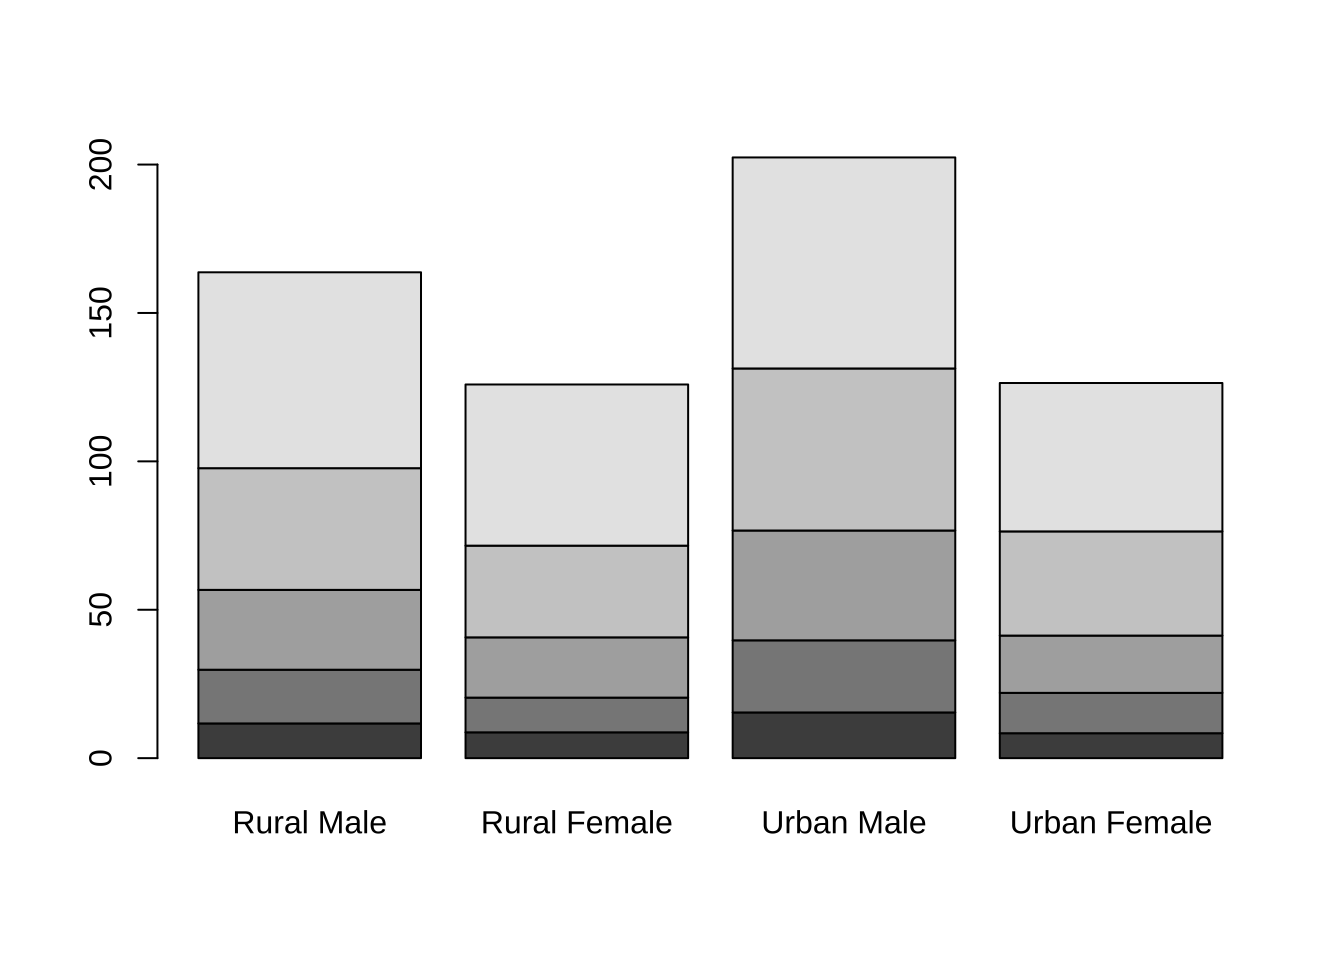
\includegraphics{1001-base-ploting_files/figure-latex/unnamed-chunk-7-1} \end{center}

\begin{Shaded}
\begin{Highlighting}[]
\FunctionTok{barplot}\NormalTok{(VADeaths, }\AttributeTok{beside =} \ConstantTok{TRUE}\NormalTok{)}
\end{Highlighting}
\end{Shaded}

\begin{center}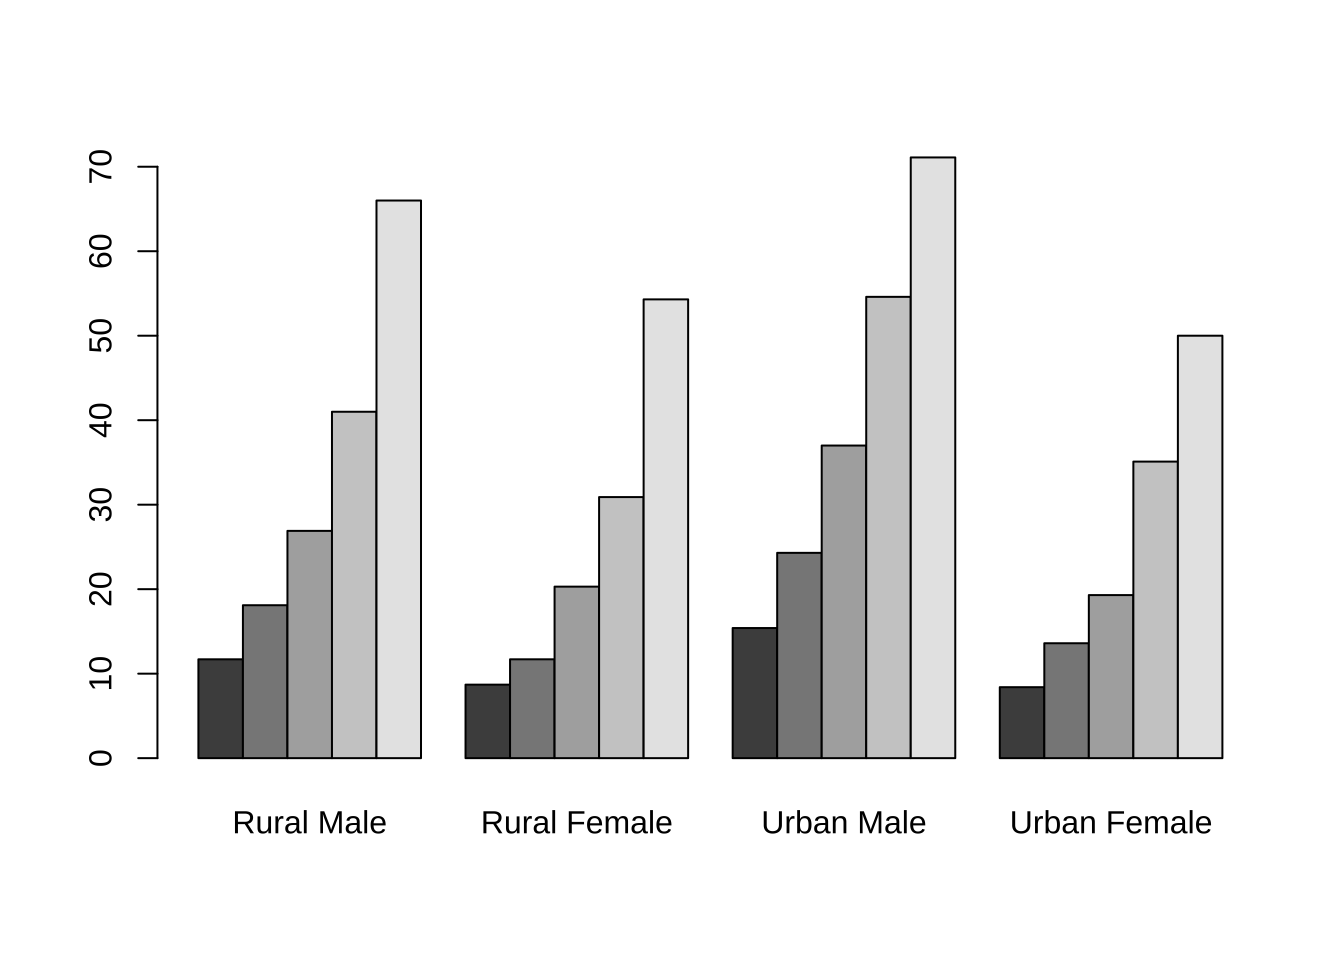
\includegraphics{1001-base-ploting_files/figure-latex/unnamed-chunk-7-2} \end{center}

\textbf{结论:}随着年龄的增长,\texttt{Viginia}人群的死亡率逐渐增加,并且在4类人群中, \texttt{Urban\ Male}的死亡率比同年龄段的其他群体的死亡率高。同时,在同一环境下,相同年龄段的男性的死亡率要比女性高。

\hypertarget{ux997cux56fe}{%
\subsubsection{饼图}\label{ux997cux56fe}}

\textbf{概念介绍}:将各项的大小与各项总和的比例。反映部分与部分、部分与整体之间的比例关系。

\textbf{例子}:

\begin{Shaded}
\begin{Highlighting}[]
\NormalTok{percent }\OtherTok{\textless{}{-}} \FunctionTok{colSums}\NormalTok{(VADeaths)}\SpecialCharTok{*}\DecValTok{100}\SpecialCharTok{/}\FunctionTok{sum}\NormalTok{(VADeaths)}
\FunctionTok{pie}\NormalTok{(percent,}\AttributeTok{labels=}\FunctionTok{paste0}\NormalTok{(}\FunctionTok{colnames}\NormalTok{(VADeaths),}\StringTok{\textquotesingle{}}\SpecialCharTok{\textbackslash{}n}\StringTok{\textquotesingle{}}\NormalTok{,}\FunctionTok{round}\NormalTok{(percent,}\DecValTok{2}\NormalTok{),}\StringTok{\textquotesingle{}\%\textquotesingle{}}\NormalTok{))}
\end{Highlighting}
\end{Shaded}

\begin{center}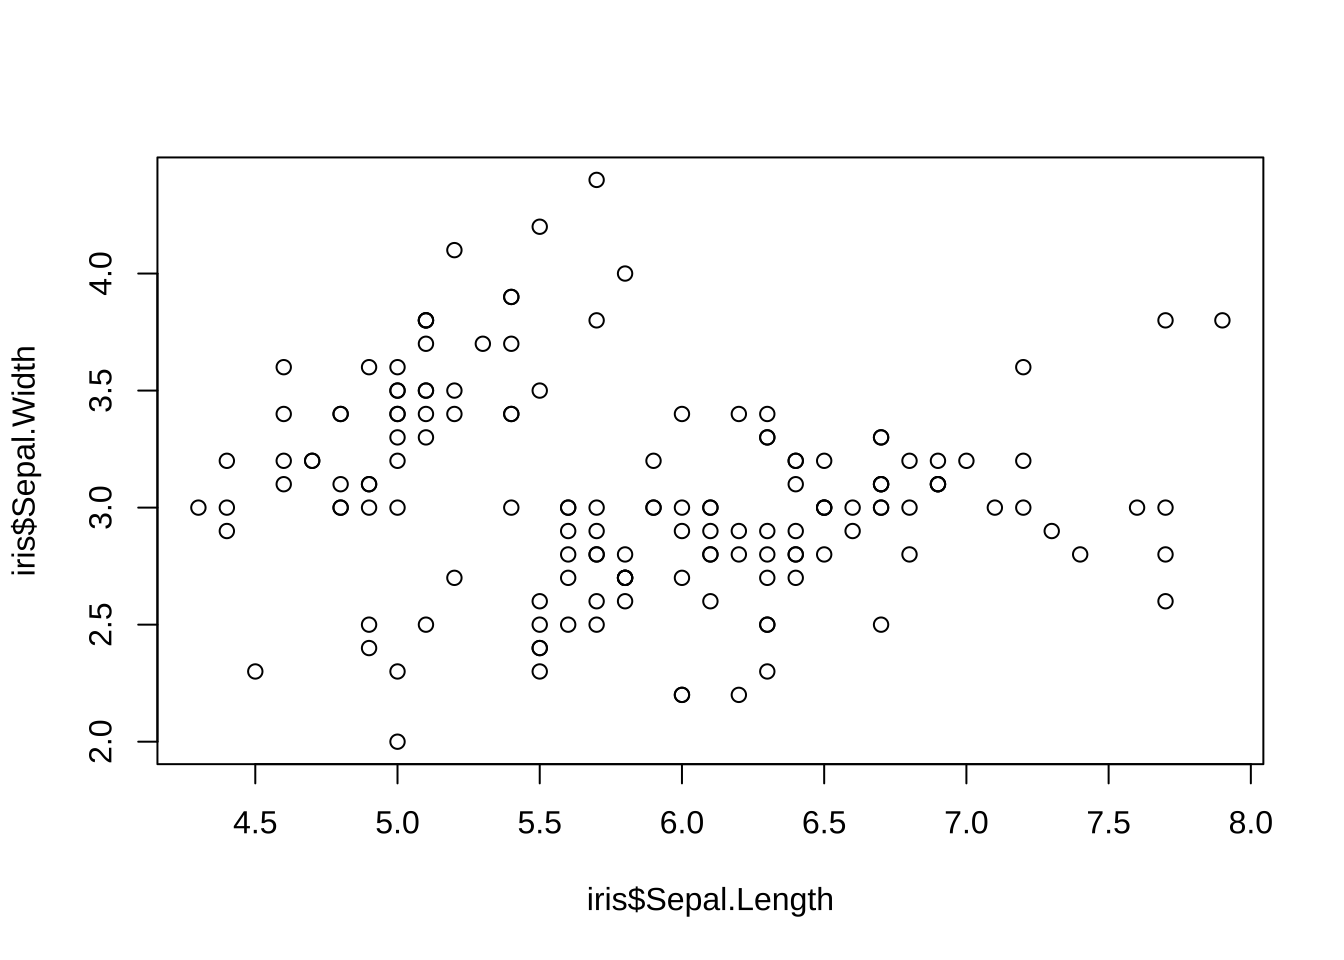
\includegraphics{1001-base-ploting_files/figure-latex/unnamed-chunk-8-1} \end{center}

\begin{Shaded}
\begin{Highlighting}[]
\FunctionTok{pie}\NormalTok{(percent,}\AttributeTok{radius=}\FloatTok{0.8}\NormalTok{) }\CommentTok{\#init.angle}
\end{Highlighting}
\end{Shaded}

\begin{center}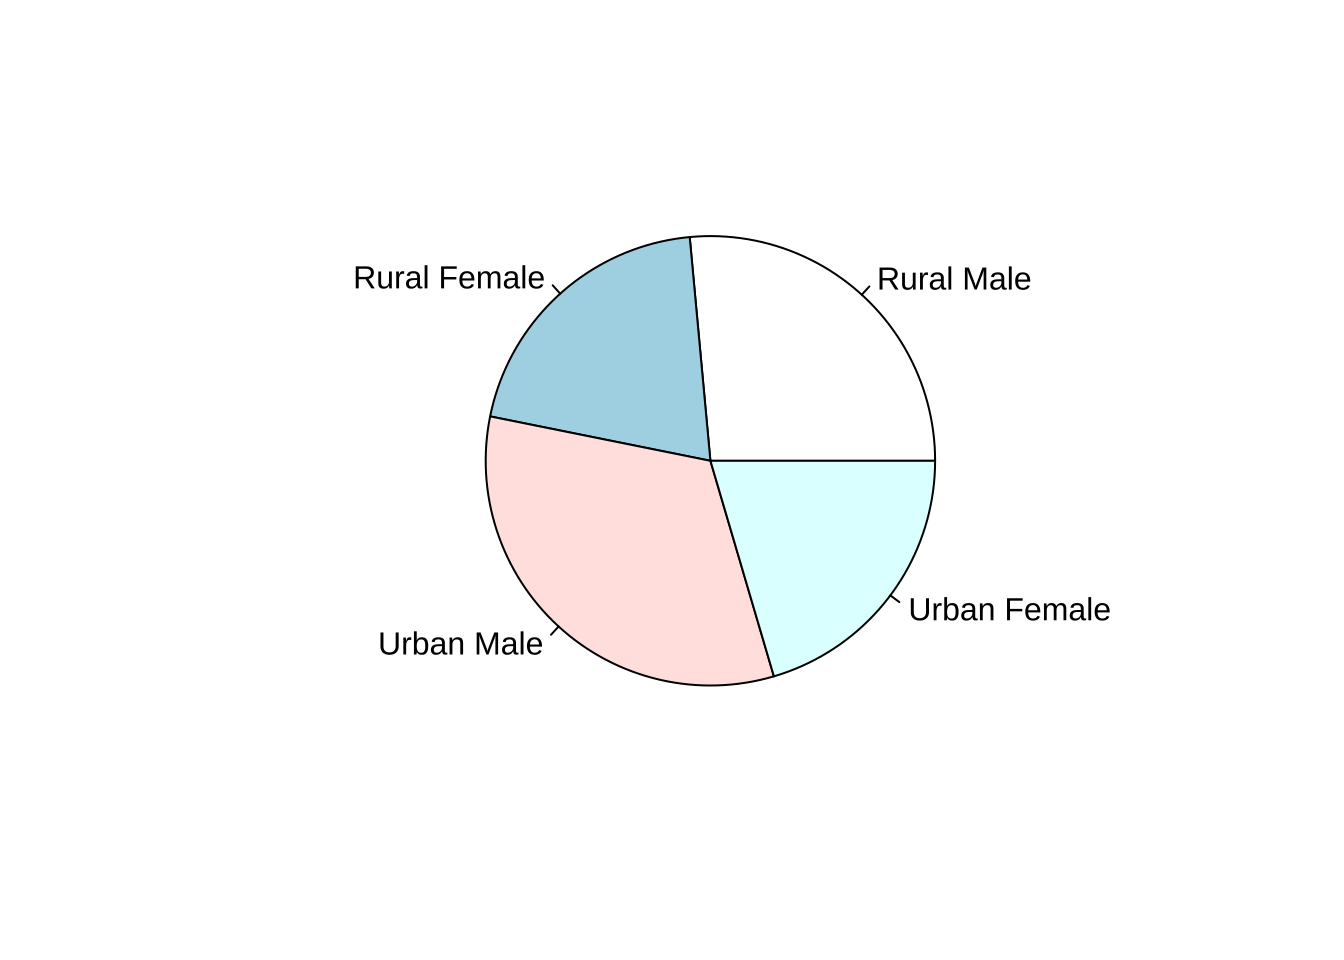
\includegraphics{1001-base-ploting_files/figure-latex/unnamed-chunk-8-2} \end{center}

\begin{Shaded}
\begin{Highlighting}[]
\CommentTok{\# ?pie}
\end{Highlighting}
\end{Shaded}

\textbf{结论:}Virginia人群中死亡最高的是Urban Male,而且男性的死亡率比女性死亡率要高。

\hypertarget{ux7bb1ux7ebfux56fe}{%
\subsubsection{箱线图}\label{ux7bb1ux7ebfux56fe}}

\textbf{概念介绍}:绘制须使用常用的统计量(最小值、下四分位数、中位数、上四分位数和最大值),并提供有关数据位置和分散情况的关键信息,尤其在比较不同特征时,更可表现其分散程度差异。

\textbf{数据介绍}:iris数据集(鸢尾花数据集),是常用的分类实验数据集合,由Fisher在1936年收集整理。数据集包含了150个子数据集,分为3类(分别为setosa、versicolor、virginica),每类50个数据,每个数据包含4个属性,即花萼长度Sepal.Length 、花萼宽度Sepal.Width、花瓣长度Petal.Length、花瓣宽度Petal.Width。

前6行数据如下:

\begin{tabular}{r|r|r|r|l}
\hline
Sepal.Length & Sepal.Width & Petal.Length & Petal.Width & Species\\
\hline
5.1 & 3.5 & 1.4 & 0.2 & setosa\\
\hline
4.9 & 3.0 & 1.4 & 0.2 & setosa\\
\hline
4.7 & 3.2 & 1.3 & 0.2 & setosa\\
\hline
4.6 & 3.1 & 1.5 & 0.2 & setosa\\
\hline
5.0 & 3.6 & 1.4 & 0.2 & setosa\\
\hline
5.4 & 3.9 & 1.7 & 0.4 & setosa\\
\hline
\end{tabular}

\textbf{例子}:
使用箱线图进行分析,使用两种方法:单独分析四个变量内部的数据分布情况;组间比较(Sepal.Length \textasciitilde{} Species)注意这里的x应该是因子型。这里没有对其他参数进行添加,大家根据自己需求添加即可。

\begin{Shaded}
\begin{Highlighting}[]
\FunctionTok{attach}\NormalTok{(iris)}
\FunctionTok{boxplot}\NormalTok{(iris[}\DecValTok{1}\SpecialCharTok{:}\DecValTok{4}\NormalTok{], }\AttributeTok{main =} \StringTok{\textquotesingle{}单独的箱线图\textquotesingle{}}\NormalTok{)}
\end{Highlighting}
\end{Shaded}

\begin{center}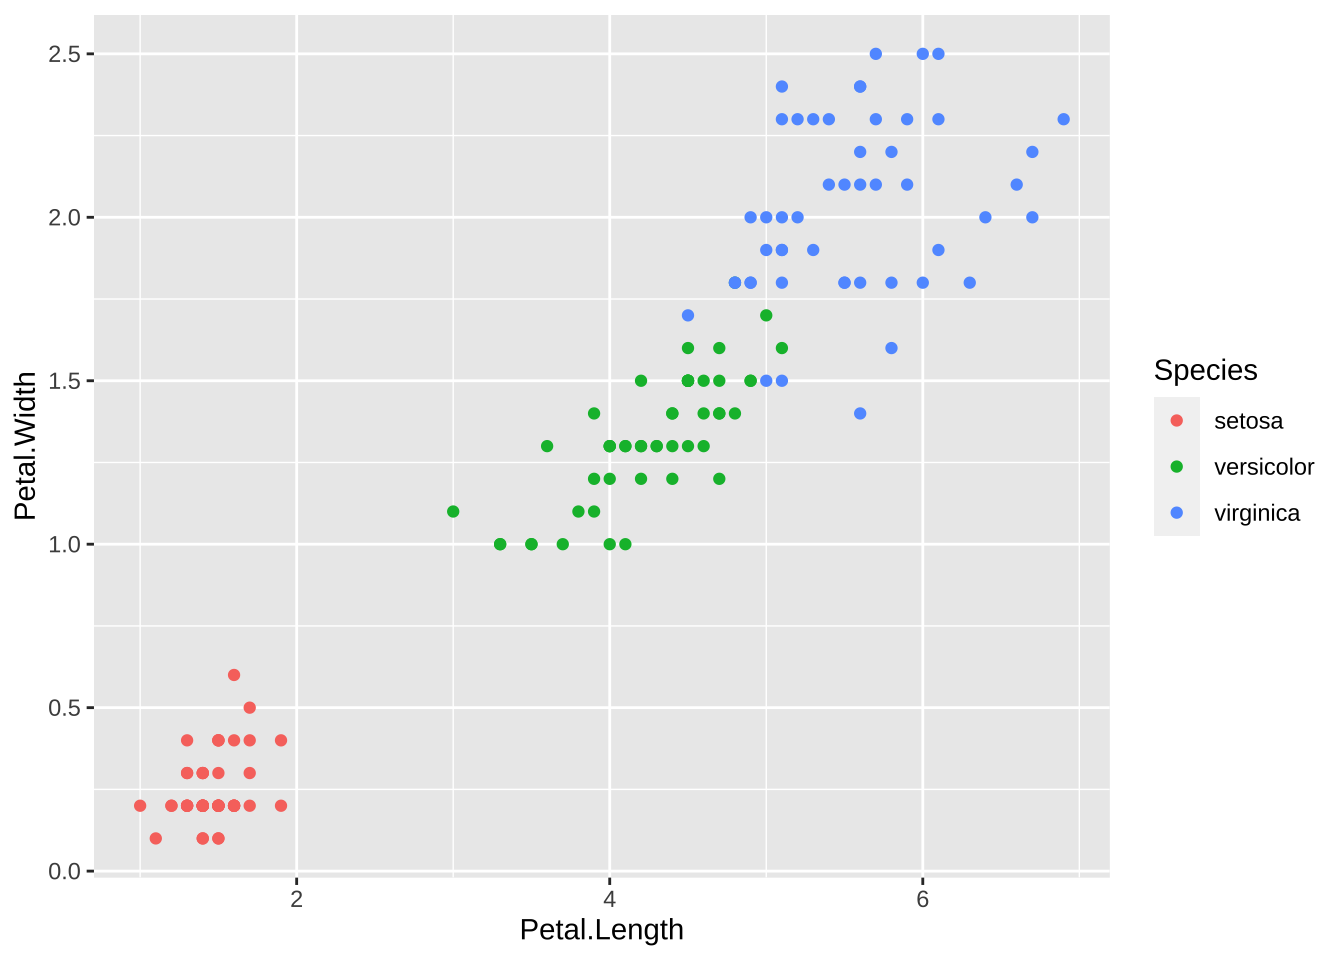
\includegraphics{1001-base-ploting_files/figure-latex/unnamed-chunk-10-1} \end{center}

\begin{Shaded}
\begin{Highlighting}[]
\FunctionTok{boxplot}\NormalTok{(Sepal.Length }\SpecialCharTok{\textasciitilde{}}\NormalTok{ Species, }\AttributeTok{data =}\NormalTok{ iris, }\AttributeTok{main =} \StringTok{\textquotesingle{}组间比较的箱线图\textquotesingle{}}\NormalTok{)}
\end{Highlighting}
\end{Shaded}

\begin{center}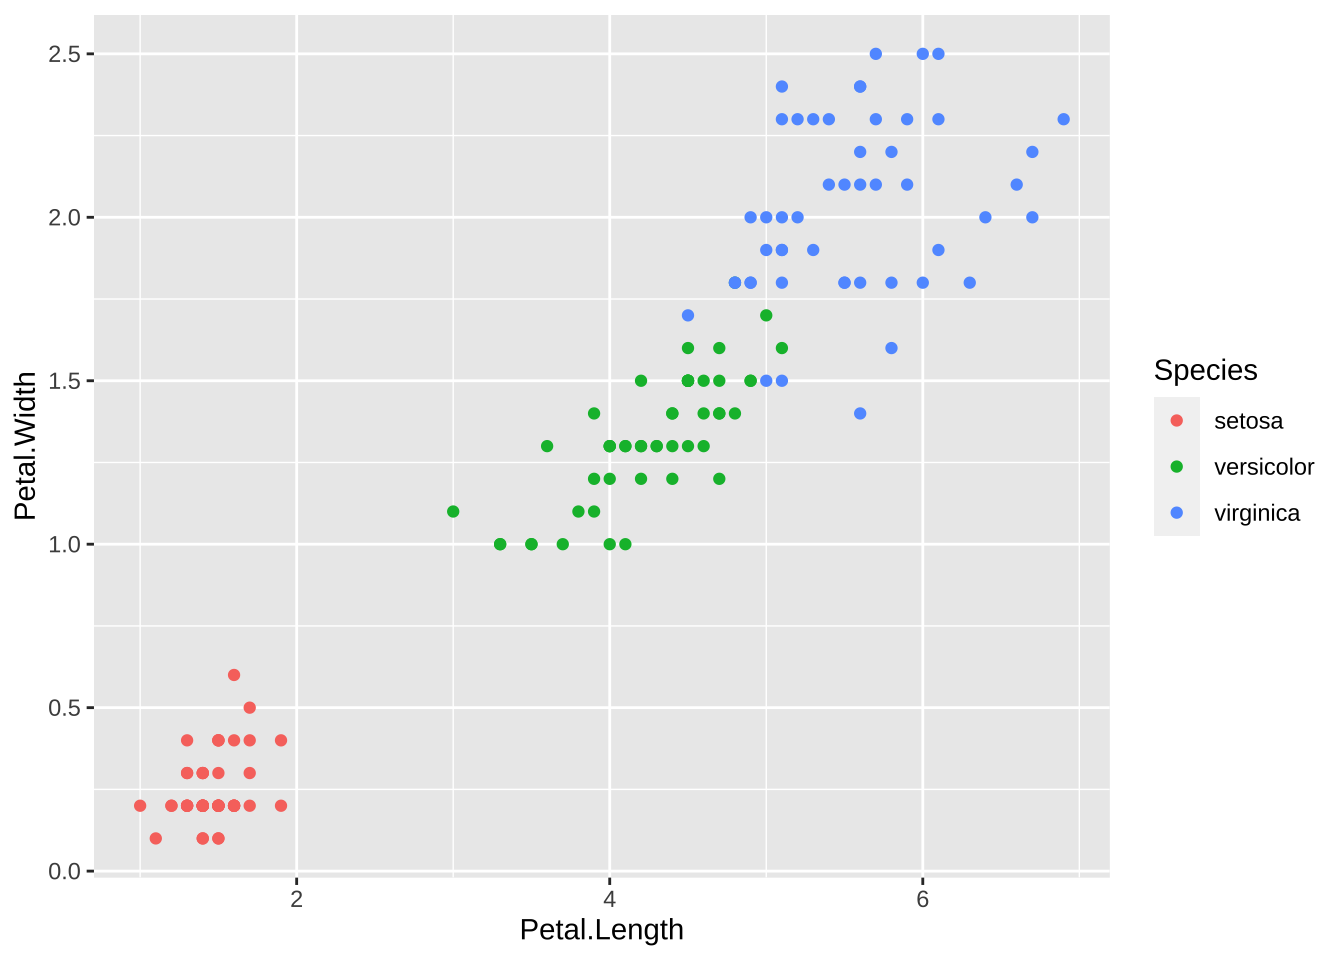
\includegraphics{1001-base-ploting_files/figure-latex/unnamed-chunk-10-2} \end{center}

\textbf{结论:}第一个图:Sepal.Width列含有四个异常值。

第二个图:Sepal.Length列中,类别属于virginica的数据含有一个异常值。同时,从第一个图可以看到,Petal.Length列前半部分相对分散,而后半部分相对密集。

\hypertarget{ux7ed8ux5236ux6570ux636eux95f4ux5173ux7cfb}{%
\subsection{绘制数据间关系}\label{ux7ed8ux5236ux6570ux636eux95f4ux5173ux7cfb}}

\textbf{概念介绍}:在分析数据间关系时,常用散点图和多变量相关矩阵图查看数据间的相关关系。

\hypertarget{ux6563ux70b9ux56fe}{%
\subsubsection{散点图}\label{ux6563ux70b9ux56fe}}

\textbf{特点:}

\begin{enumerate}
\def\labelenumi{(\arabic{enumi})}
\item
  特征之间是否存在关联趋势,关联趋势是线性的还是非线性的。
\item
  一目了然的看出离群值。从而可以进一步分析这些离群值是否可能在建模分析中产生很大的影响。
\end{enumerate}

\textbf{例子}:使用cars数据进行分析速度(speed)和刹车距离(dist)之间的关系

\begin{Shaded}
\begin{Highlighting}[]
\FunctionTok{plot}\NormalTok{(cars[, }\DecValTok{1}\NormalTok{], cars[, }\DecValTok{2}\NormalTok{],}\AttributeTok{xlab =} \StringTok{"speed"}\NormalTok{,}\AttributeTok{ylab =} \StringTok{"dist"}\NormalTok{)}
\end{Highlighting}
\end{Shaded}

\begin{center}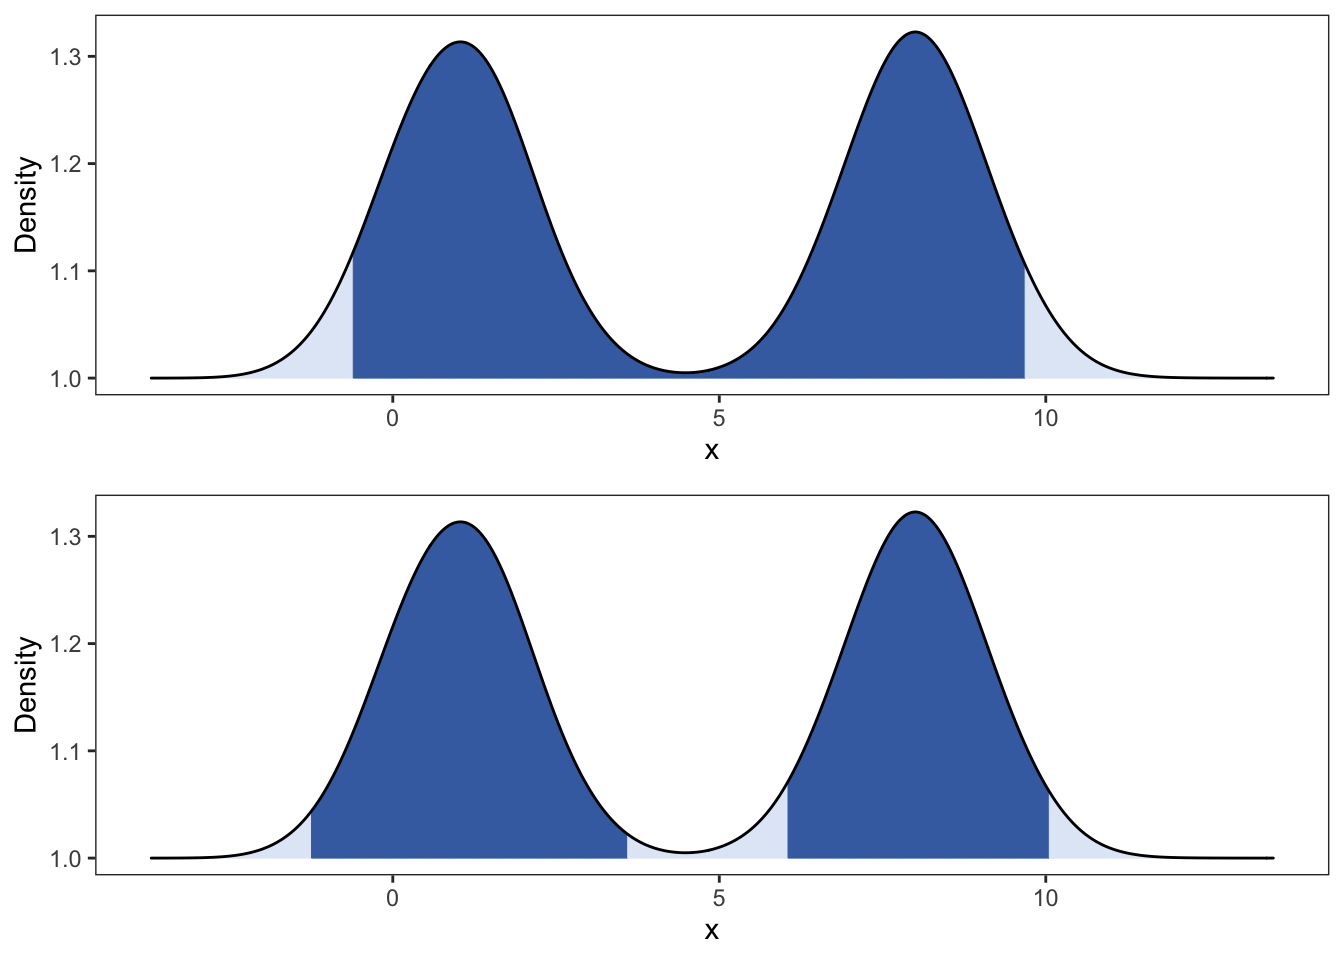
\includegraphics{1001-base-ploting_files/figure-latex/unnamed-chunk-11-1} \end{center}

\begin{Shaded}
\begin{Highlighting}[]
\CommentTok{\# plot(cars)  \# 效果同上}
\end{Highlighting}
\end{Shaded}

\textbf{结论:}随着汽车行驶速度的增加,刹车距离也在不断增加。

\hypertarget{ux6563ux70b9ux77e9ux9635ux56fe}{%
\subsubsection{散点矩阵图}\label{ux6563ux70b9ux77e9ux9635ux56fe}}

\textbf{概念介绍}:散点矩阵图将多个散点图组合起来,以便可以同时浏览多个二元变量关系,一定程度上克服了在平面上展示高维数据分布情况的困难。可以使用\texttt{plot()}或者\texttt{pairs()}进行绘制。

\textbf{适用}:高维数据

\begin{itemize}
\tightlist
\item
  \textbf{plot}
\end{itemize}

\begin{Shaded}
\begin{Highlighting}[]
\FunctionTok{plot}\NormalTok{(iris[,}\DecValTok{1}\SpecialCharTok{:}\DecValTok{4}\NormalTok{]) }
\end{Highlighting}
\end{Shaded}

\begin{center}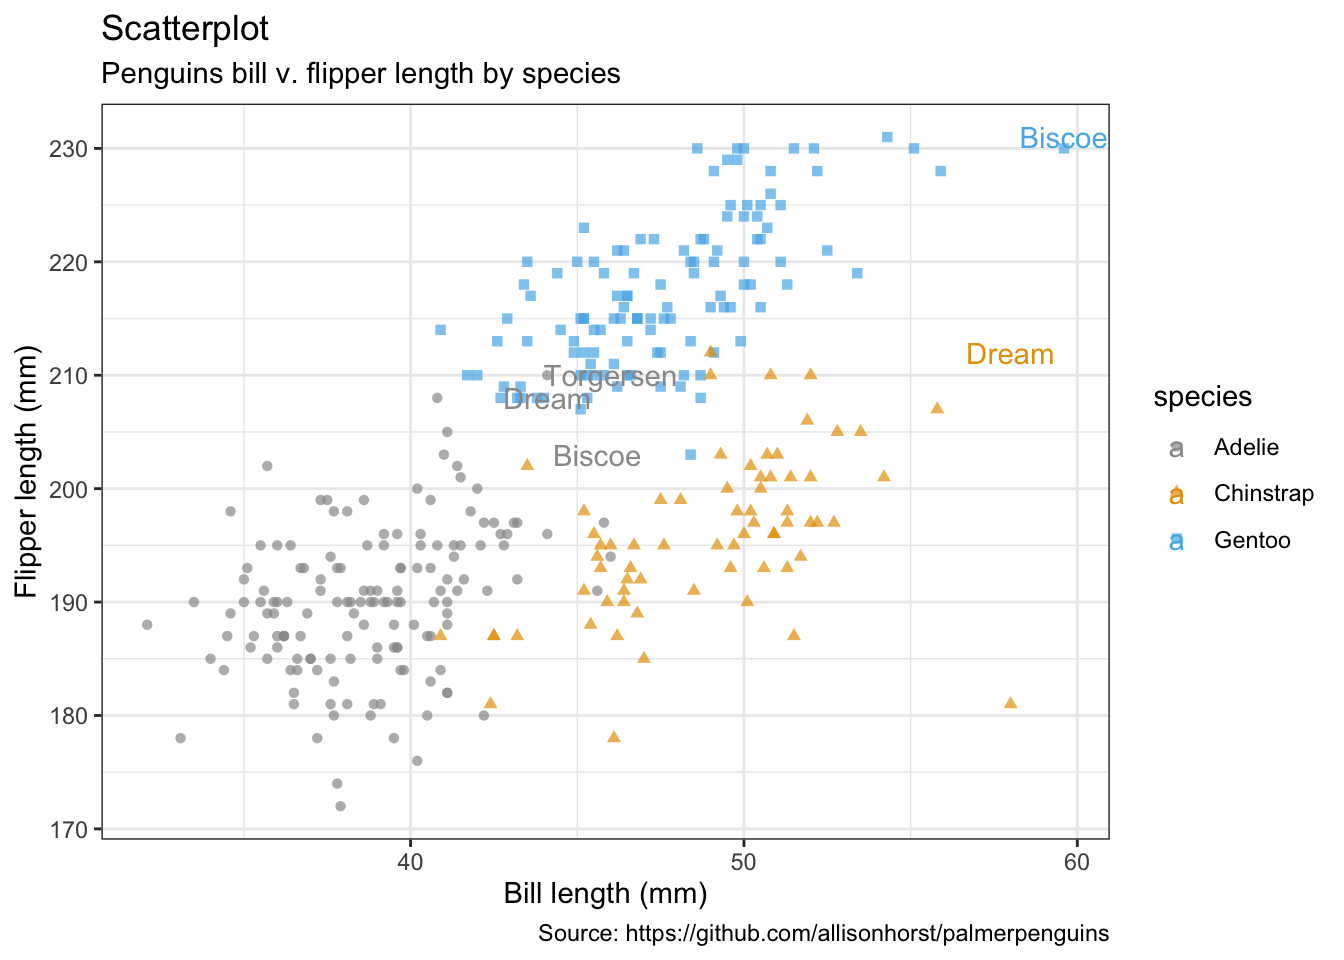
\includegraphics{1001-base-ploting_files/figure-latex/unnamed-chunk-12-1} \end{center}

\textbf{结论:}花瓣长度(Petal.length)与花瓣宽度(Petal.Width)有明显的线性关系,其余属性之间的关系不是很明显。

\begin{itemize}
\tightlist
\item
  \textbf{pairs}
\end{itemize}

此外,R中还提供了另一个绘制散点矩阵图的函数------pairs函数,绘图对象有\textbf{数据框}和\textbf{公式}两种:

\begin{Shaded}
\begin{Highlighting}[]
\FunctionTok{pairs}\NormalTok{(iris[,}\DecValTok{1}\SpecialCharTok{:}\DecValTok{4}\NormalTok{])}
\FunctionTok{pairs}\NormalTok{(}\SpecialCharTok{\textasciitilde{}}\NormalTok{Sepal.Length }\SpecialCharTok{+}\NormalTok{ Sepal.Width }\SpecialCharTok{+}\NormalTok{ Petal.Length }\SpecialCharTok{+}\NormalTok{ Petal.Width, }\AttributeTok{data =}\NormalTok{ iris)  }\CommentTok{\# 效果同上}
\end{Highlighting}
\end{Shaded}

\begin{center}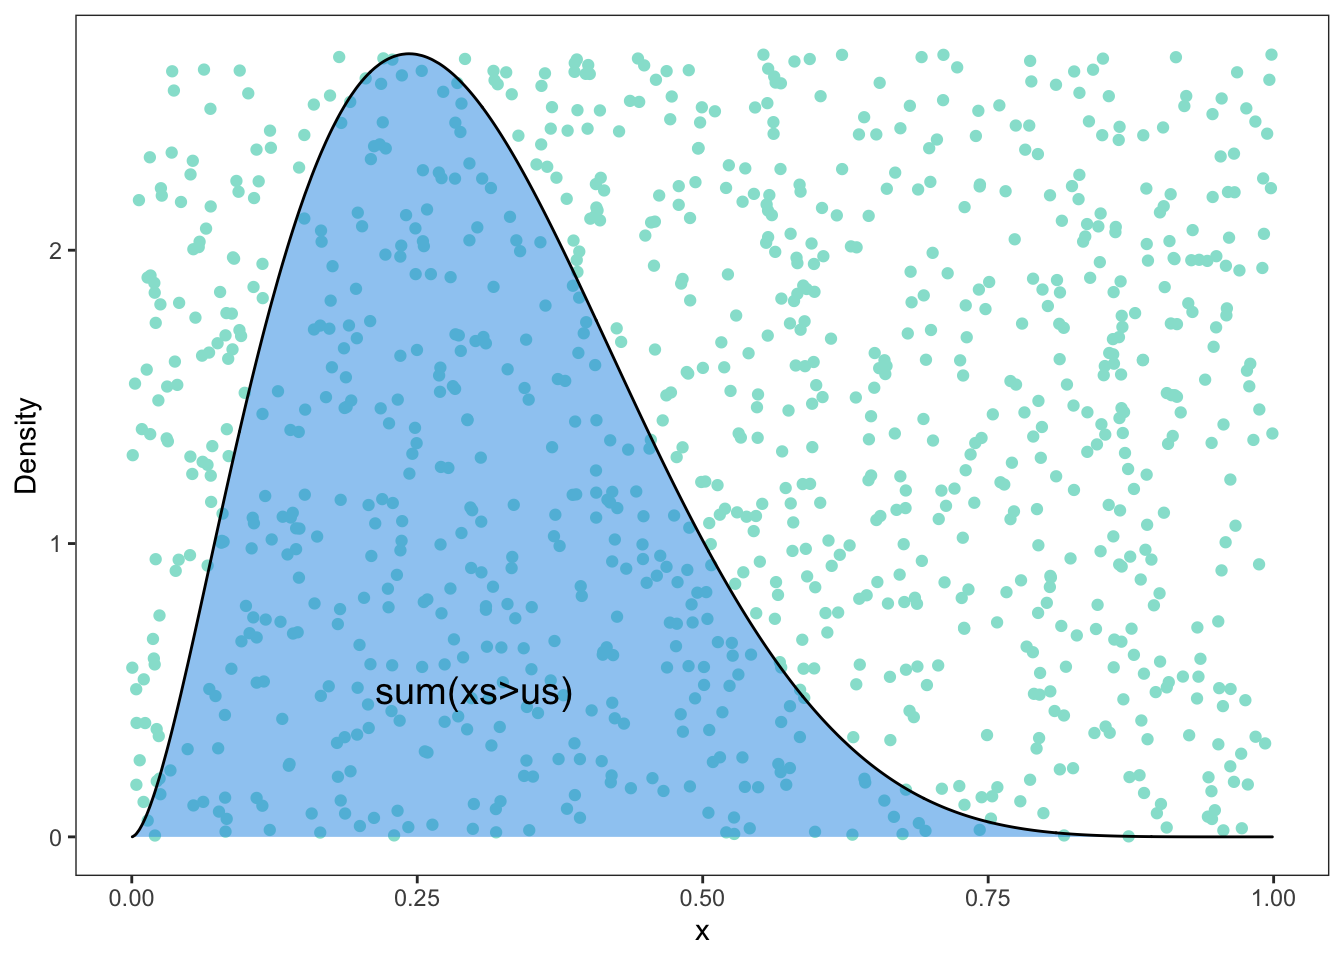
\includegraphics{1001-base-ploting_files/figure-latex/unnamed-chunk-13-1} \end{center}

\hypertarget{ux591aux53d8ux91cfux76f8ux5173ux77e9ux9635ux56fe}{%
\subsubsection{多变量相关矩阵图}\label{ux591aux53d8ux91cfux76f8ux5173ux77e9ux9635ux56fe}}

\textbf{概念介绍}:多变量相关矩阵图是\textbf{相关系数矩阵}(correlation matrix)的可视化结果,显示了两两变量间的相关关系,对数据维度相对较大的数据有较好的展示效果。在R的\texttt{corrgram}包中的\texttt{corrgram}函数可绘制多变量相关矩阵图。

\textbf{数据介绍}:Mtcar数据集是1974年Motor Trend US杂志公布的32辆车的11个数据,包括燃料消耗和10个关于汽车设计与性能的数据。

\textbf{例子}:下面、根据这个数据集,绘制适用中不同元素描述相关性大小的图。

\begin{Shaded}
\begin{Highlighting}[]
\FunctionTok{library}\NormalTok{(corrgram) }
\FunctionTok{corrgram}\NormalTok{(mtcars)}
\end{Highlighting}
\end{Shaded}

\begin{center}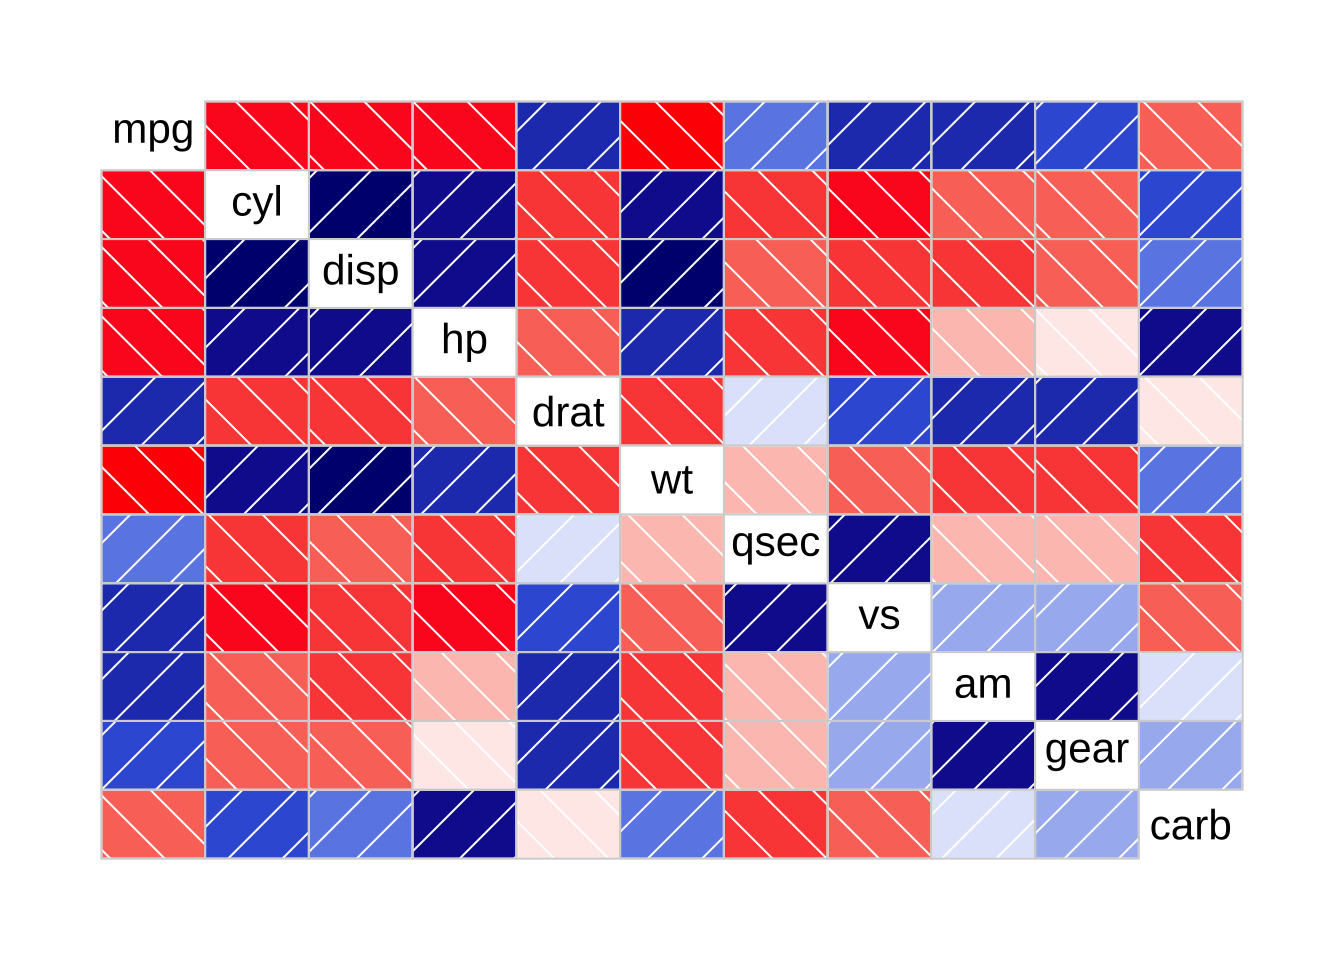
\includegraphics{1001-base-ploting_files/figure-latex/unnamed-chunk-14-1} \end{center}

\begin{Shaded}
\begin{Highlighting}[]
\FunctionTok{corrgram}\NormalTok{(mtcars, }\AttributeTok{order=}\ConstantTok{TRUE}\NormalTok{, }\AttributeTok{upper.panel=}\NormalTok{panel.ellipse, }
         \AttributeTok{main=}\StringTok{"Correlogram of mtcars intercorrelations"}\NormalTok{) }
\end{Highlighting}
\end{Shaded}

\begin{center}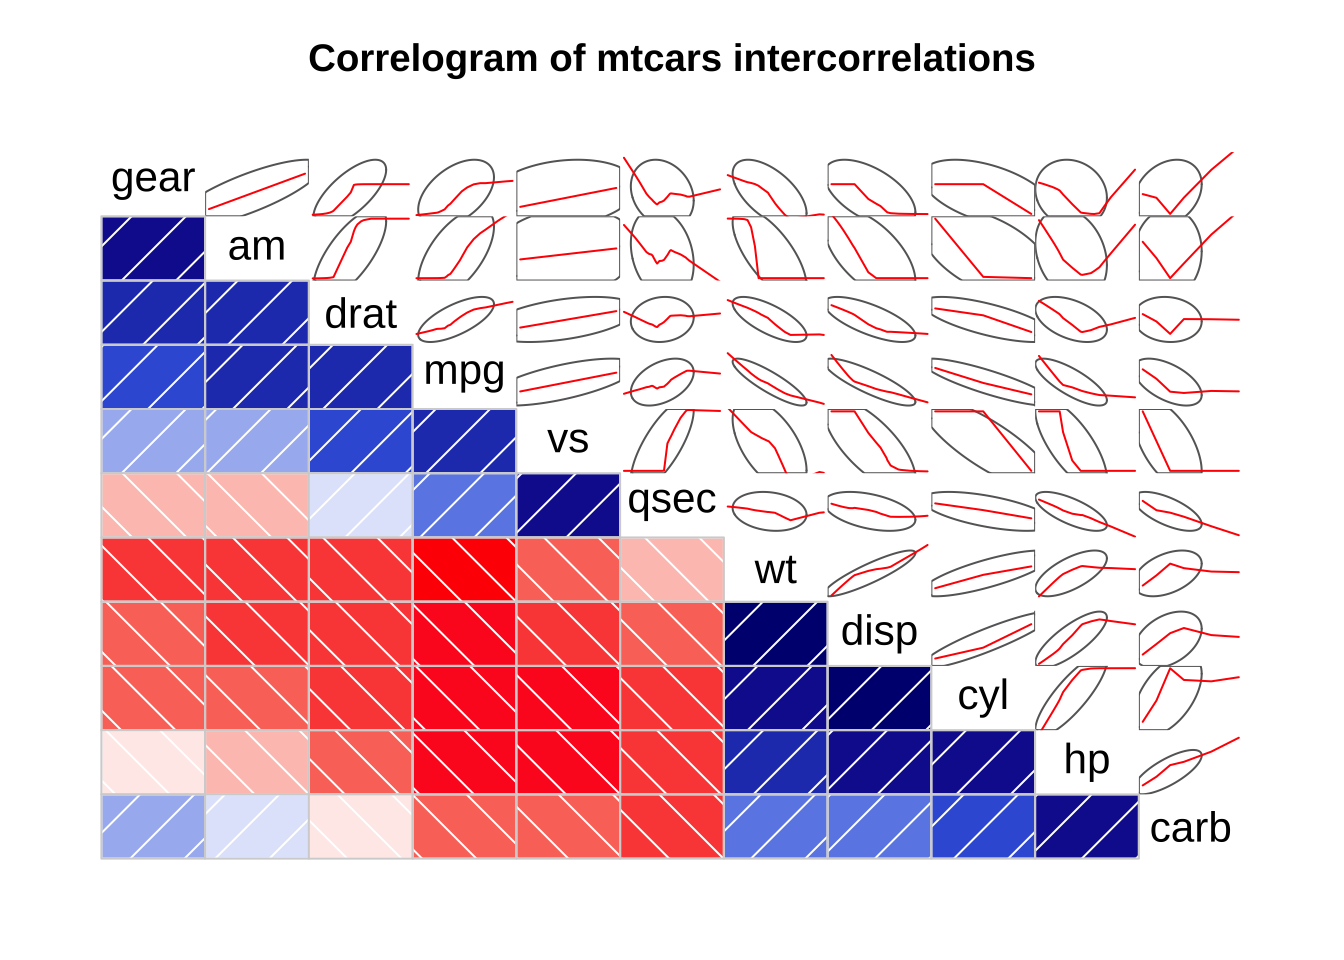
\includegraphics{1001-base-ploting_files/figure-latex/unnamed-chunk-14-2} \end{center}

\begin{Shaded}
\begin{Highlighting}[]
\CommentTok{\# 相关图,主对角线上方绘制置信椭圆和平滑拟合曲线,主对角线下方绘制阴影}
\end{Highlighting}
\end{Shaded}

\textbf{结论}:\texttt{disp}与\texttt{cyl}呈正相关关系,且相关程度较高。此外,\texttt{mpg}与\texttt{wt}呈高度负相关,且\texttt{am}与\texttt{carb}基本没有关系。

这里可以对\texttt{upper.panel}和\texttt{lower.panel}进行设置,展示不同图形。具体可以通过帮助获得相信参数设置信息(\texttt{?corrgram})

\begin{Shaded}
\begin{Highlighting}[]
\CommentTok{\# 相关图,主对角线上方绘制散点图,主对角线下方绘制饼图}
\FunctionTok{corrgram}\NormalTok{(mtcars, }\AttributeTok{order=}\ConstantTok{TRUE}\NormalTok{, }\AttributeTok{upper.panel=}\NormalTok{panel.pts, }\AttributeTok{lower.panel=}\NormalTok{panel.pie, }
         \AttributeTok{main=}\StringTok{"Correlogram of mtcars intercorrelations"}\NormalTok{) }
\end{Highlighting}
\end{Shaded}

\begin{center}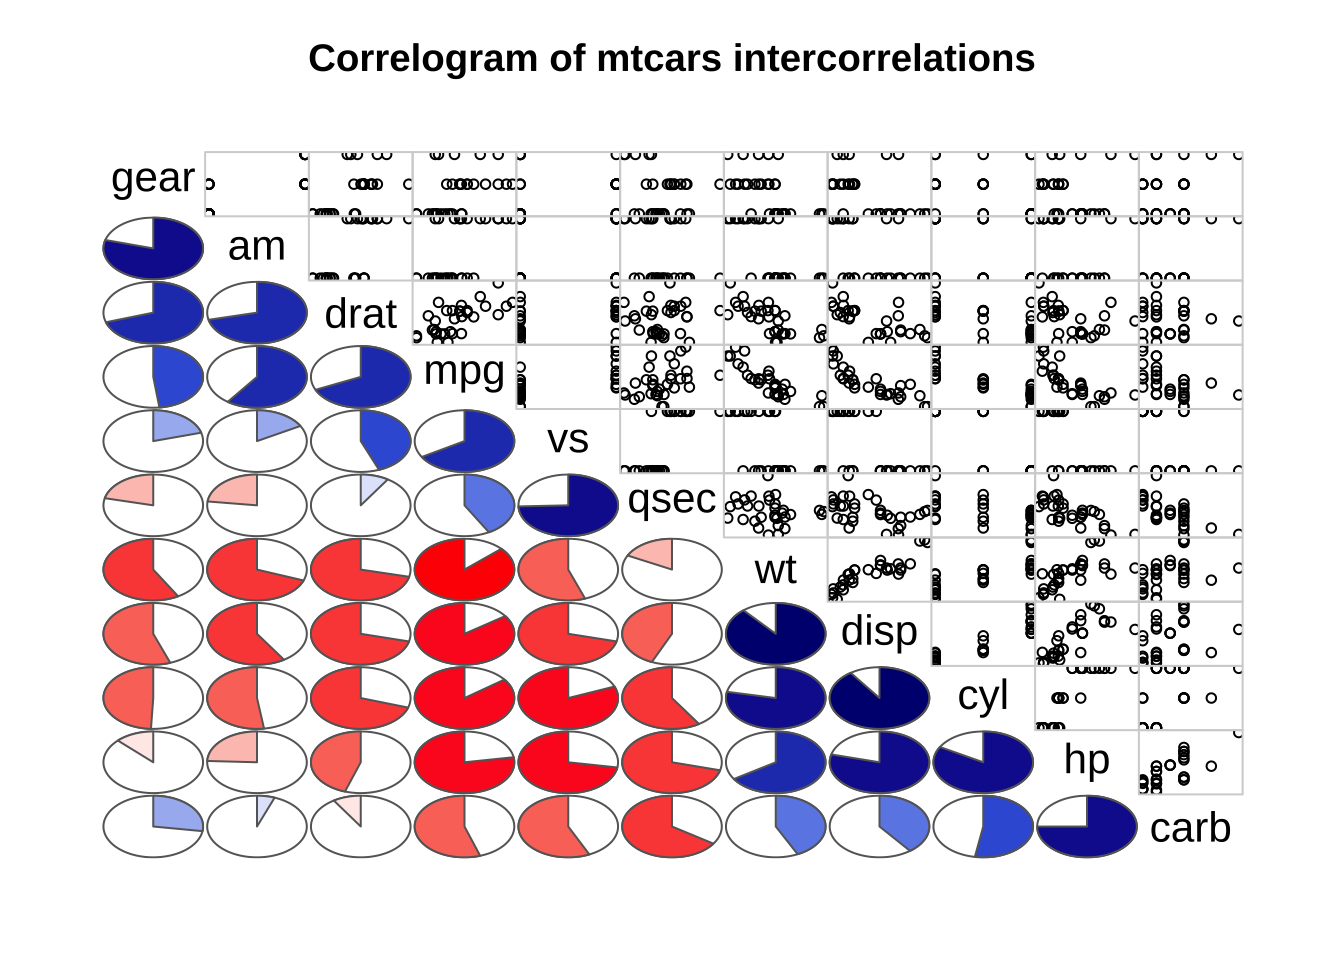
\includegraphics{1001-base-ploting_files/figure-latex/unnamed-chunk-15-1} \end{center}

\begin{Shaded}
\begin{Highlighting}[]
\CommentTok{\# 相关图,主对角线上方绘制置信区间,主对角线下方绘制相关系数}
\FunctionTok{corrgram}\NormalTok{(mtcars, }\AttributeTok{order=}\ConstantTok{TRUE}\NormalTok{, }\AttributeTok{upper.panel=}\NormalTok{panel.conf, }\AttributeTok{lower.panel=}\NormalTok{panel.cor,}
         \AttributeTok{main=}\StringTok{"Correlogram of mtcars intercorrelations"}\NormalTok{) }
\end{Highlighting}
\end{Shaded}

\begin{center}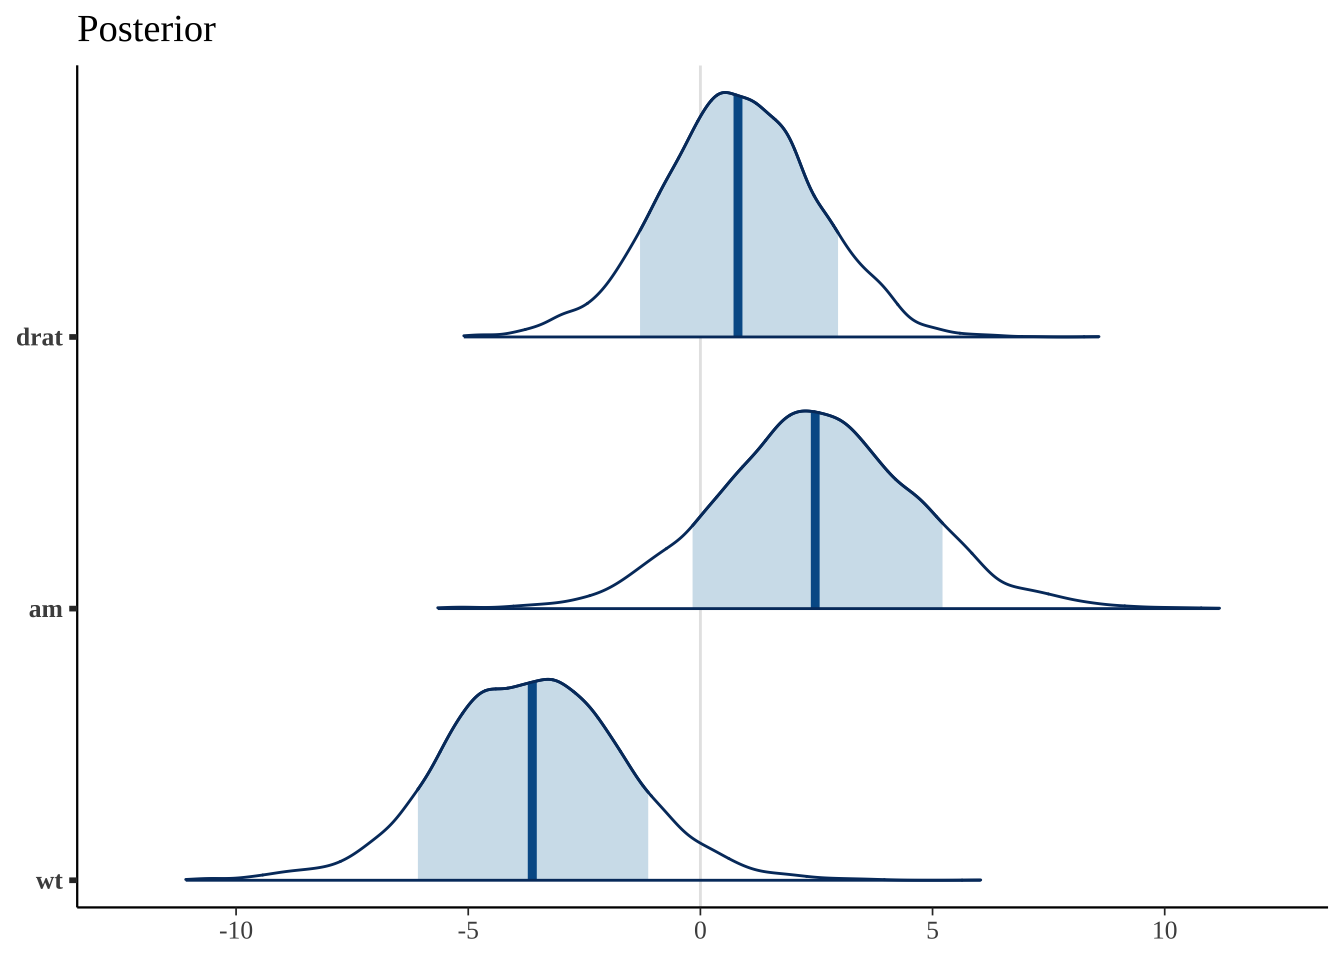
\includegraphics{1001-base-ploting_files/figure-latex/unnamed-chunk-16-1} \end{center}

\hypertarget{ux7ed8ux5236ux5176ux4ed6ux56feux5f62}{%
\subsection{绘制其他图形}\label{ux7ed8ux5236ux5176ux4ed6ux56feux5f62}}

\hypertarget{ux6838ux5bc6ux5ea6ux56fe}{%
\subsubsection{核密度图}\label{ux6838ux5bc6ux5ea6ux56fe}}

\textbf{概念介绍}:sm包中\texttt{sm.density.compare}函数用于绘制核密度图,核密度图如果想用一条密度曲线而不是通过柱状来展示连续型变量的分布。

\textbf{特点}:相比直方图,密度图的一个优势是可以堆放,可用于比较组间差异。\texttt{sm.density.compare}函数可以直接堆放多条密度曲线。使用格式如下。

\texttt{sm.density.compare(x\ ,group,….)}

其中x是数值向量,group是分组向量,是因子型数据。

\begin{Shaded}
\begin{Highlighting}[]
\FunctionTok{library}\NormalTok{(sm)      }\CommentTok{\# 加载sm包}
\FunctionTok{sm.density.compare}\NormalTok{(mtcars}\SpecialCharTok{$}\NormalTok{wt, }\FunctionTok{factor}\NormalTok{(mtcars}\SpecialCharTok{$}\NormalTok{cyl))     }\CommentTok{\# 绘制核密度图}
\end{Highlighting}
\end{Shaded}

\begin{center}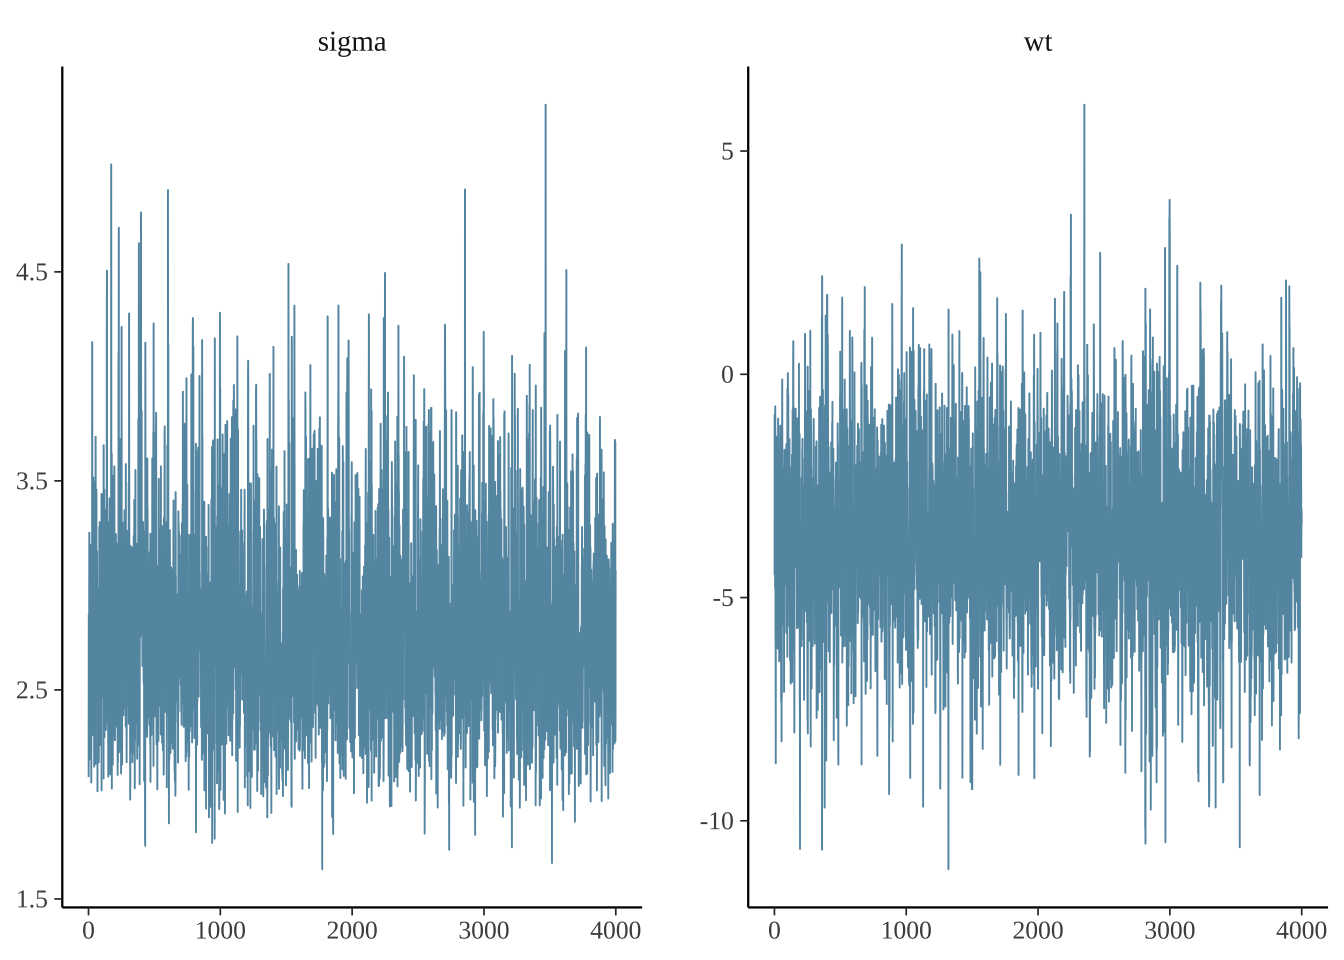
\includegraphics{1001-base-ploting_files/figure-latex/unnamed-chunk-17-1} \end{center}

\hypertarget{ux5c0fux63d0ux7434ux56fe}{%
\subsubsection{小提琴图}\label{ux5c0fux63d0ux7434ux56fe}}

\textbf{概念介绍}:vioplot包中的vioplot函数用于绘制小提琴图,小提琴图是核密度图与箱线图的结合,本质是利用密度值生成的多边形,但该多边形同时还沿着一条直线作了另一半对称的``镜像'',这样两个左右或上下对称的多边形拼起来就形成了小提琴图的主体部分,最后一个箱线图也会被添加在小提琴的中轴线上。

使用格式如下。

\texttt{vioplot(\ x\ ,\ ...,\ \ range=1.5,\ \ h,\ \ ylim,\ names,\ \ horizontal=FALSE\ ,\ …)}

其中,x为数据源,可以是向量;range默认等于1.5;col是为每幅小提琴图指定颜色的向量。

\begin{Shaded}
\begin{Highlighting}[]
\FunctionTok{library}\NormalTok{(vioplot)      }\CommentTok{\# 加载vioplot包}
\FunctionTok{attach}\NormalTok{(mtcars)}
\FunctionTok{vioplot}\NormalTok{(wt[cyl}\SpecialCharTok{==}\DecValTok{4}\NormalTok{], wt[cyl}\SpecialCharTok{==}\DecValTok{6}\NormalTok{], wt[cyl}\SpecialCharTok{==}\DecValTok{8}\NormalTok{],  }\AttributeTok{border=}\StringTok{"black"}\NormalTok{, }
        \AttributeTok{col =} \StringTok{"gray60"}\NormalTok{, }\AttributeTok{rectCol =} \StringTok{"blue"}\NormalTok{, }\AttributeTok{horizontal =} \ConstantTok{TRUE}\NormalTok{,}
        \AttributeTok{main =} \StringTok{\textquotesingle{}小提琴图\textquotesingle{}}\NormalTok{)  }\CommentTok{\# 绘制小提琴图}
\end{Highlighting}
\end{Shaded}

\begin{center}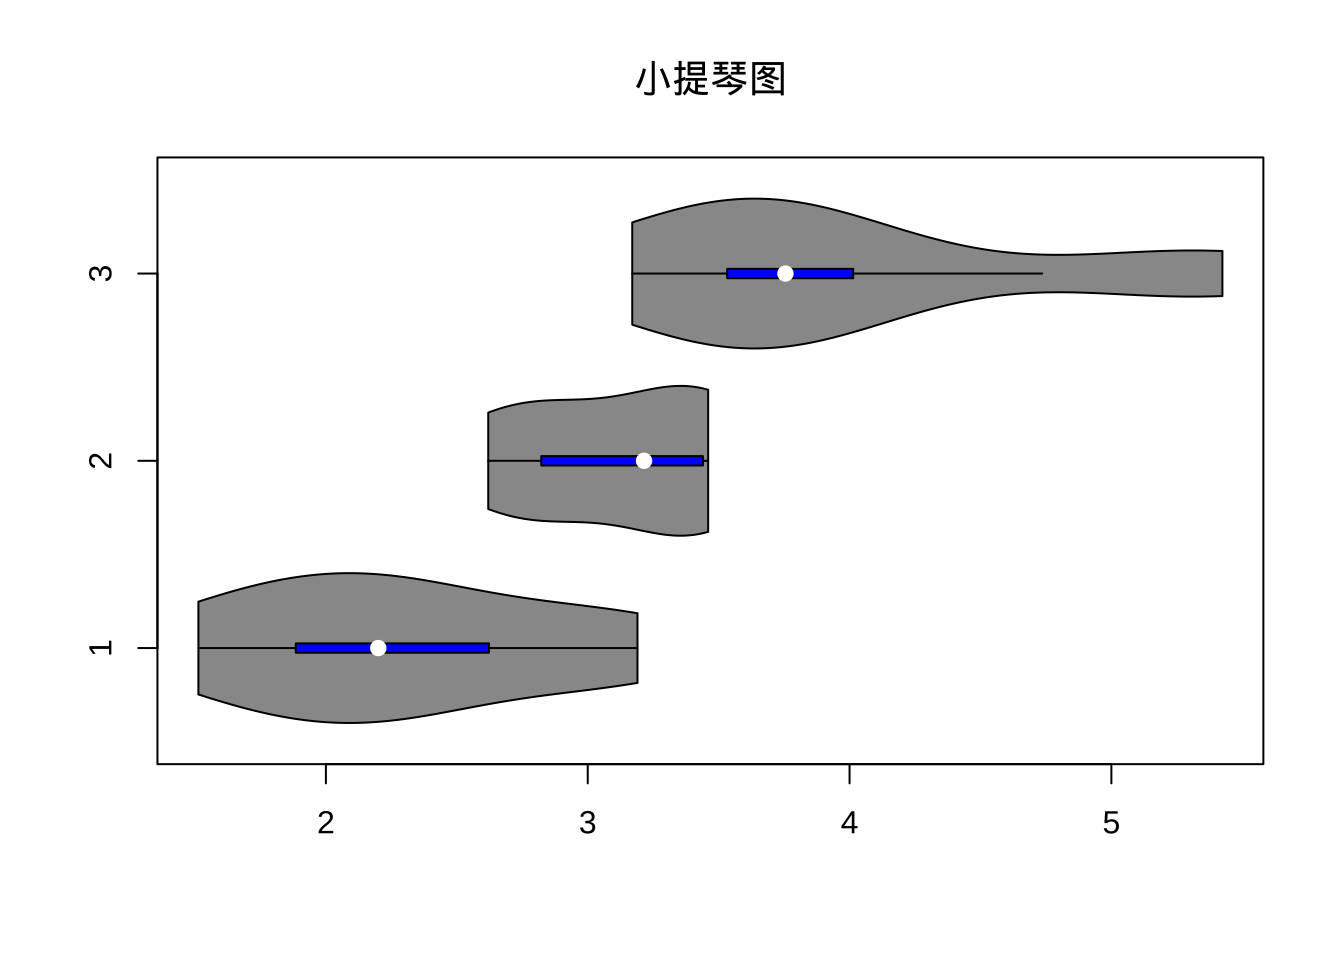
\includegraphics{1001-base-ploting_files/figure-latex/unnamed-chunk-18-1} \end{center}

\begin{Shaded}
\begin{Highlighting}[]
\FunctionTok{boxplot}\NormalTok{(wt}\SpecialCharTok{\textasciitilde{}}\NormalTok{cyl, }\AttributeTok{main =} \StringTok{\textquotesingle{}箱线图\textquotesingle{}}\NormalTok{, }\AttributeTok{horizontal=}\ConstantTok{TRUE}\NormalTok{,}
        \AttributeTok{pars=}\FunctionTok{list}\NormalTok{(}\AttributeTok{boxwex=}\FloatTok{0.1}\NormalTok{), }\AttributeTok{border=}\StringTok{"blue"}\NormalTok{)  }\CommentTok{\# 绘制箱线图}
\end{Highlighting}
\end{Shaded}

\begin{center}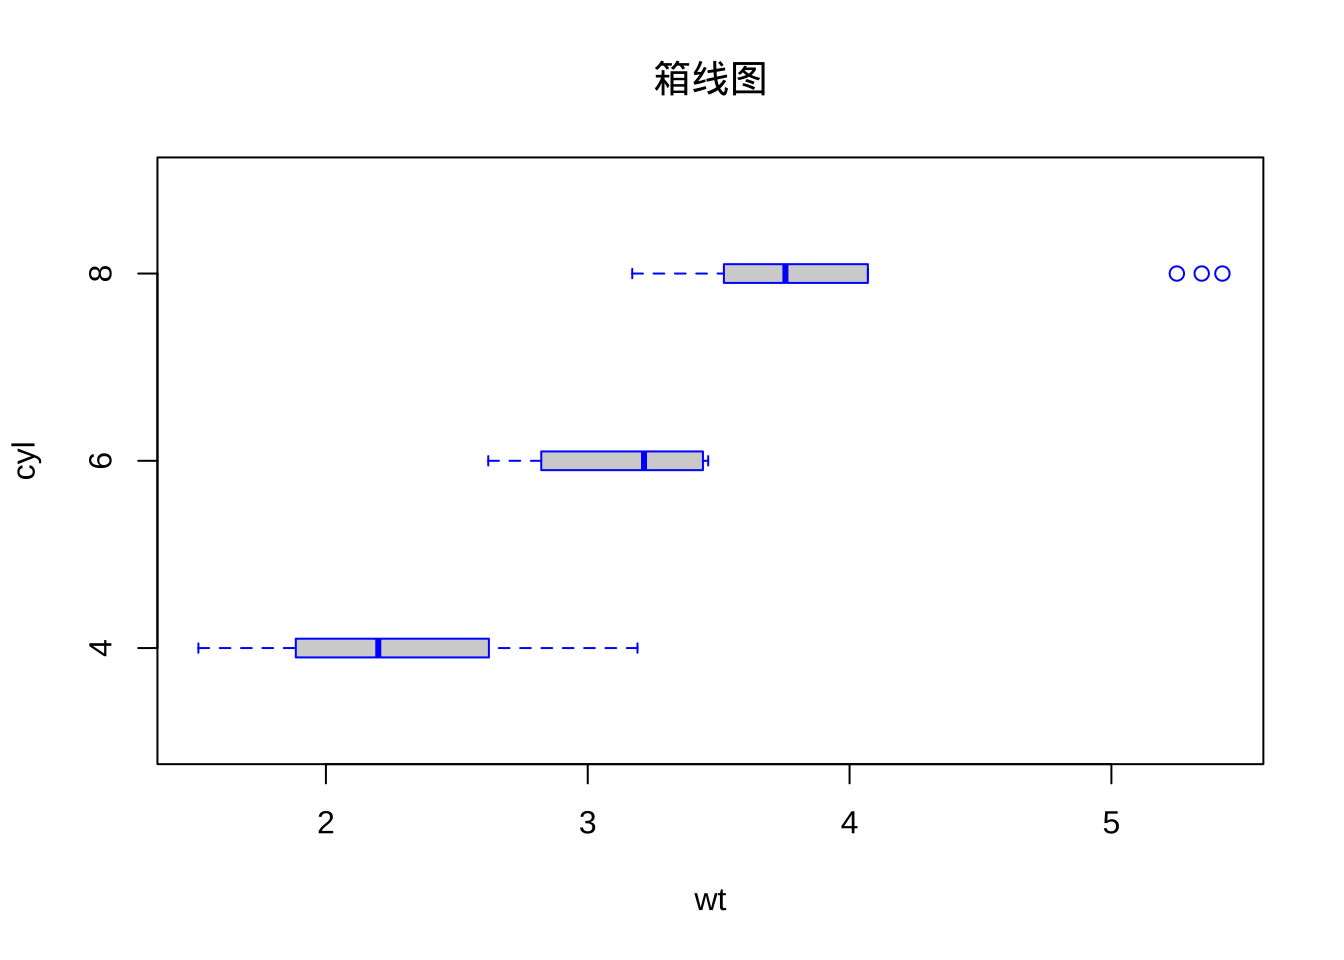
\includegraphics{1001-base-ploting_files/figure-latex/unnamed-chunk-18-2} \end{center}

\hypertarget{qqux56fe}{%
\subsubsection{QQ图}\label{qqux56fe}}

\textbf{概念介绍}:查看经验分布和理论分布是否一致。将排序后的数据和理论分布的分位数进行比较后大致相等,说明了经验分布和理论分布相似。\texttt{qqplot()}函数用于绘制QQ图,QQ图检查数据是否服从某种分布。

使用格式如下:

\texttt{qqplot(x,\ y,,...);qqnorm(y,…)\ ;\ qqline(y)}

其中,x与y均为数据源,可以是向量。

\begin{Shaded}
\begin{Highlighting}[]
\FunctionTok{qqnorm}\NormalTok{(wt)     }\CommentTok{\#正态分布QQ图}
\FunctionTok{qqline}\NormalTok{(wt)      }\CommentTok{\#QQ线}
\end{Highlighting}
\end{Shaded}

\begin{center}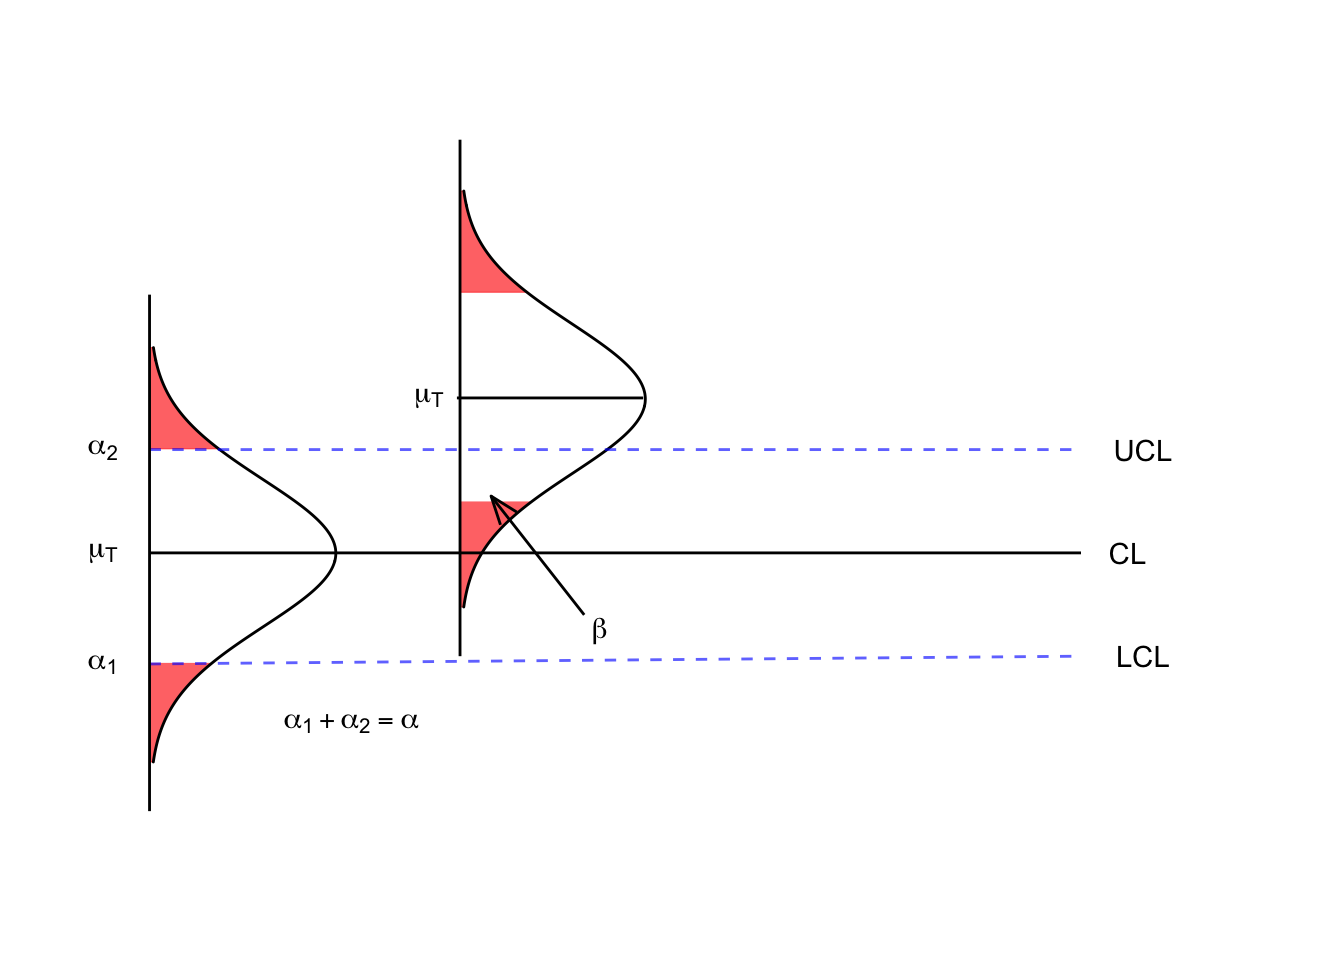
\includegraphics{1001-base-ploting_files/figure-latex/unnamed-chunk-19-1} \end{center}

\hypertarget{ux7b49ux9ad8ux56fe}{%
\subsubsection{等高图}\label{ux7b49ux9ad8ux56fe}}

\textbf{概念介绍}:数据形式:两个数值向量x、y和一个相应的矩阵z。x、y交叉组合之后形成的是一个``网格'',z是这个网格上的高度数值,将平面上对应的z值(高度)相等的点连接起来形成的线就是等高线。对x、y进行核密度估计,得到一个密度值矩阵,然后用x、y以及这个密度值矩阵作等高图。由于密度值反映的是某个位置上数据的密集程度,等高图就展示了一个聚类现象。

使用格式如下

\texttt{contour(x=,y=,z,nlevels=,levels=,labels=\ ,method=,...)}

\begin{Shaded}
\begin{Highlighting}[]
\FunctionTok{library}\NormalTok{(KernSmooth)  }\CommentTok{\# 计算二维核密度的包}
\NormalTok{mtcars1 }\OtherTok{=} \FunctionTok{data.frame}\NormalTok{(wt, mpg)}
\NormalTok{est }\OtherTok{=} \FunctionTok{bkde2D}\NormalTok{(mtcars1, }\FunctionTok{apply}\NormalTok{(mtcars1, }\DecValTok{2}\NormalTok{, dpik))     }\CommentTok{\# 计算二维核密度}
\FunctionTok{contour}\NormalTok{(est}\SpecialCharTok{$}\NormalTok{x1, est}\SpecialCharTok{$}\NormalTok{x2, est}\SpecialCharTok{$}\NormalTok{fhat, }\AttributeTok{nlevels =} \DecValTok{15}\NormalTok{, }
        \AttributeTok{col =} \StringTok{"darkgreen"}\NormalTok{, }\AttributeTok{xlab =} \StringTok{"wt"}\NormalTok{, }\AttributeTok{ylab =} \StringTok{"mpg"}\NormalTok{)  }\CommentTok{\# 画等高图}
\FunctionTok{points}\NormalTok{(mtcars1)  }\CommentTok{\# 添加散点}
\end{Highlighting}
\end{Shaded}

\begin{center}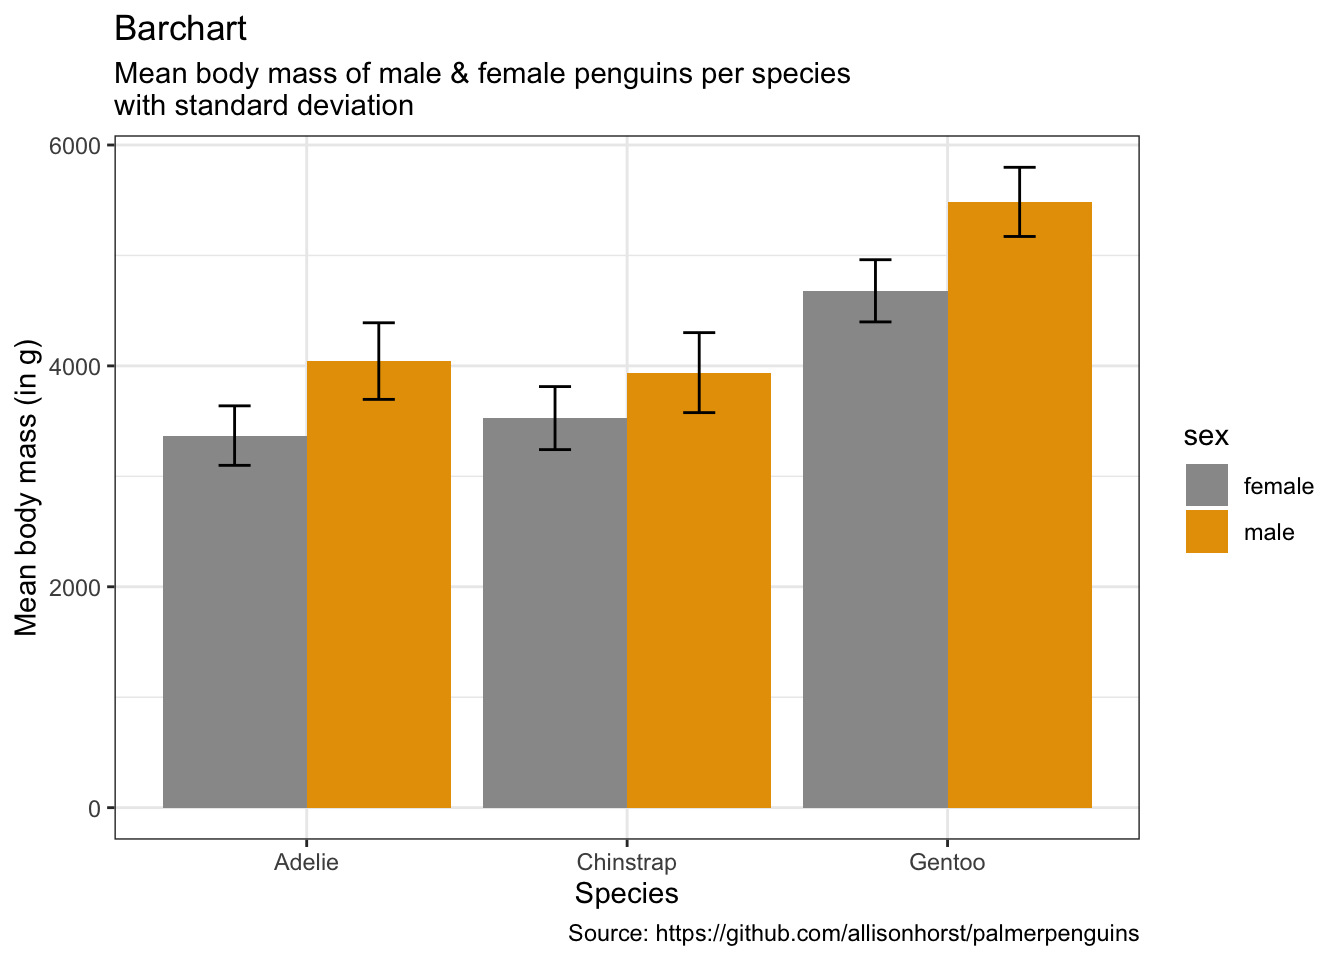
\includegraphics{1001-base-ploting_files/figure-latex/unnamed-chunk-20-1} \end{center}

\hypertarget{ux4feeux6539ux56feux5f62ux53c2ux6570}{%
\section{修改图形参数}\label{ux4feeux6539ux56feux5f62ux53c2ux6570}}

R是一个功能强大的图形构建平台,可以通过逐条输入语句构建图形元素(\textbf{颜色、点、线、文本以及图例}等),逐渐完善图形特征,直至得到想要的效果。图形元素的显示可以用图形函数和绘图参数来改良,也可以用绘制图形元素的基础函数来控制。

\hypertarget{ux4feeux6539ux989cux8272}{%
\subsection{修改颜色}\label{ux4feeux6539ux989cux8272}}

R语言通过设置绘图参数col来改变\textbf{图像、坐标轴、文字、点、线}等的颜色。关于颜色的函数大致可以分为下面三类:

\hypertarget{ux56faux5b9aux989cux8272ux9009ux62e9ux51fdux6570}{%
\subsubsection{固定颜色选择函数}\label{ux56faux5b9aux989cux8272ux9009ux62e9ux51fdux6570}}

R语言提供了自带的固定种类的颜色,主要涉及的是colors函数,该函数可以生成657中颜色名称,代表657种颜色,可以通过以下代码查看R自带颜色的前20中颜色的名称。

\begin{Shaded}
\begin{Highlighting}[]
\FunctionTok{colors}\NormalTok{()[}\DecValTok{1}\SpecialCharTok{:}\DecValTok{20}\NormalTok{] }
\end{Highlighting}
\end{Shaded}

\begin{verbatim}
##  [1] "white"         "aliceblue"     "antiquewhite"  "antiquewhite1"
##  [5] "antiquewhite2" "antiquewhite3" "antiquewhite4" "aquamarine"   
##  [9] "aquamarine1"   "aquamarine2"   "aquamarine3"   "aquamarine4"  
## [13] "azure"         "azure1"        "azure2"        "azure3"       
## [17] "azure4"        "beige"         "bisque"        "bisque1"
\end{verbatim}

\begin{Shaded}
\begin{Highlighting}[]
\CommentTok{\# colors()}
\FunctionTok{plot}\NormalTok{(}\DecValTok{1}\SpecialCharTok{:}\DecValTok{10}\NormalTok{,}\AttributeTok{col =} \FunctionTok{cm.colors}\NormalTok{(}\DecValTok{1}\NormalTok{))}
\end{Highlighting}
\end{Shaded}

\begin{center}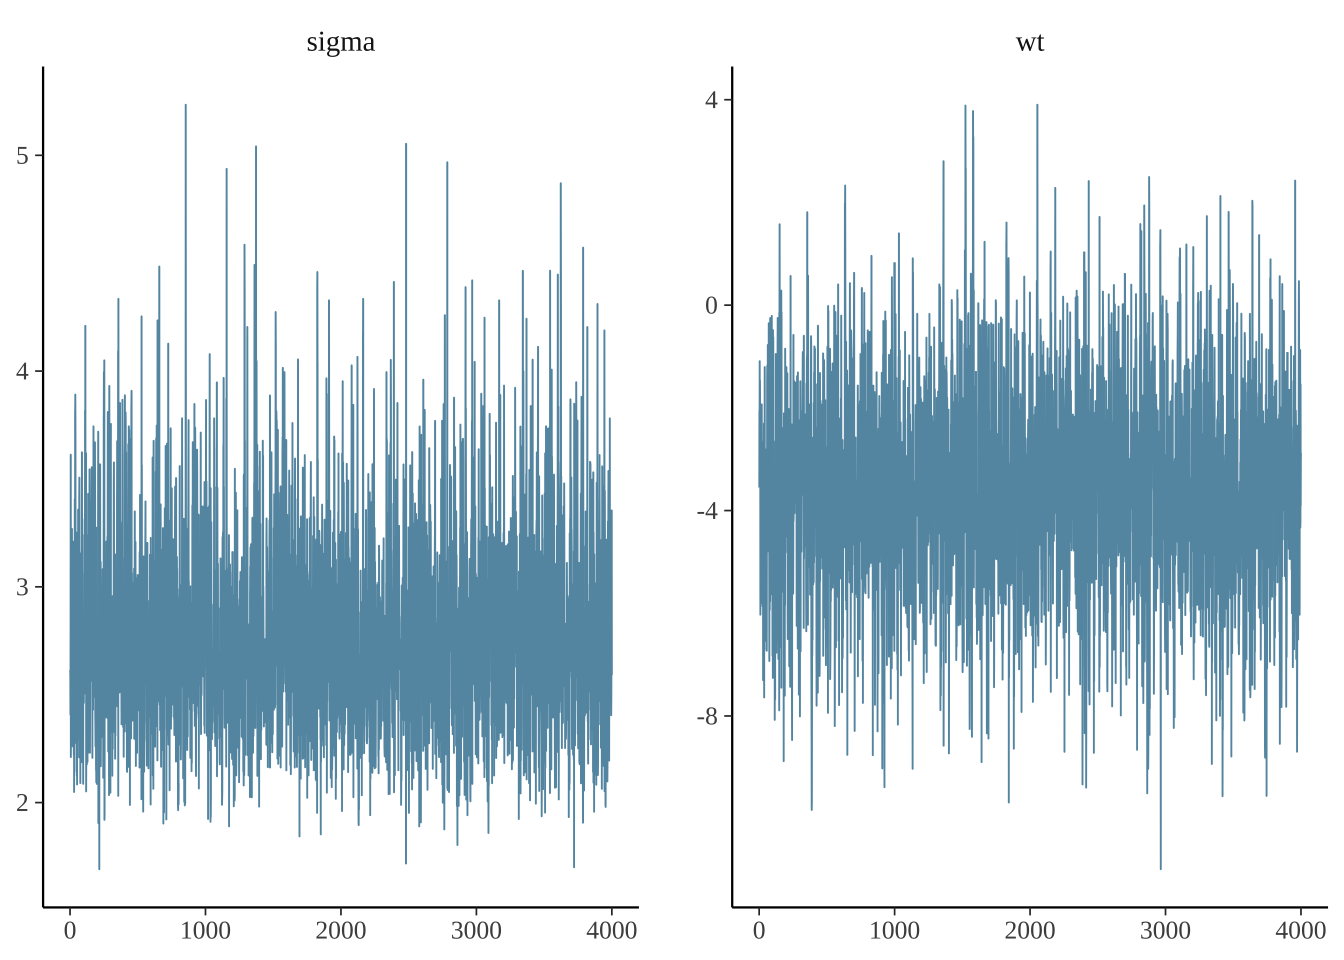
\includegraphics{1001-base-ploting_files/figure-latex/unnamed-chunk-21-1} \end{center}

通过palette函数固定调色板,只要设定好了调色板,它的取值就不会再改变(直到下一次重新设定调色板)。

\begin{Shaded}
\begin{Highlighting}[]
\FunctionTok{palette}\NormalTok{() }\CommentTok{\#返回当前的调色板设置,此时为默认值}
\DocumentationTok{\#\# [1] "black"   "\#DF536B" "\#61D04F" "\#2297E6" "\#28E2E5" "\#CD0BBC" "\#F5C710"}
\DocumentationTok{\#\# [8] "gray62"}
\FunctionTok{palette}\NormalTok{(}\FunctionTok{colors}\NormalTok{()[}\DecValTok{1}\SpecialCharTok{:}\DecValTok{10}\NormalTok{]) }\CommentTok{\#重新设置调色板为colors的前10种颜色}
\FunctionTok{palette}\NormalTok{()               }\CommentTok{\#返回当前的调色板设置,此时为colors()的前10种颜色}
\DocumentationTok{\#\#  [1] "white"         "aliceblue"     "antiquewhite"  "antiquewhite1"}
\DocumentationTok{\#\#  [5] "antiquewhite2" "antiquewhite3" "antiquewhite4" "aquamarine"   }
\DocumentationTok{\#\#  [9] "aquamarine"    "aquamarine2"}
\FunctionTok{palette}\NormalTok{(}\StringTok{\textquotesingle{}default\textquotesingle{}}\NormalTok{) }\CommentTok{\#恢复默认的调色板设置}
\end{Highlighting}
\end{Shaded}

\textbf{例子}:

\begin{Shaded}
\begin{Highlighting}[]
\FunctionTok{plot}\NormalTok{(iris}\SpecialCharTok{$}\NormalTok{Sepal.Length, iris}\SpecialCharTok{$}\NormalTok{Sepal.Width, }\AttributeTok{col =}\NormalTok{ iris}\SpecialCharTok{$}\NormalTok{Species)  }
\end{Highlighting}
\end{Shaded}

\begin{center}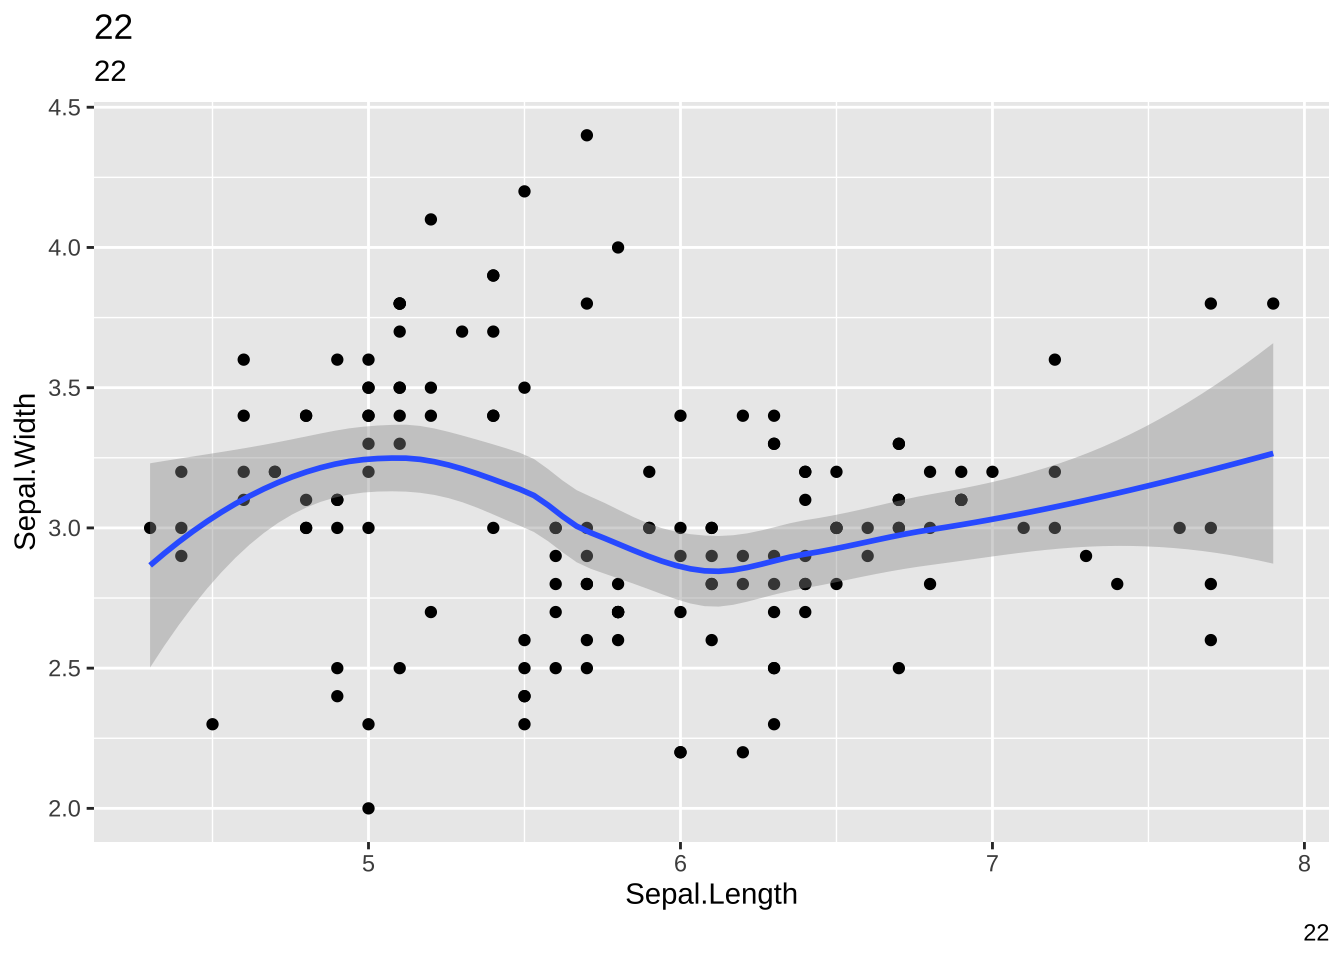
\includegraphics{1001-base-ploting_files/figure-latex/unnamed-chunk-23-1} \end{center}

\begin{Shaded}
\begin{Highlighting}[]
\CommentTok{\# Species为因子型数据,setosa versicolor virginica分别对应数字1,2,3,}
\CommentTok{\# 即等价于col = rep(1:3, each = 50)}
\end{Highlighting}
\end{Shaded}

\hypertarget{ux6e10ux53d8ux8272ux751fux6210ux51fdux6570}{%
\subsubsection{渐变色生成函数}\label{ux6e10ux53d8ux8272ux751fux6210ux51fdux6570}}

除了固定颜色选择函数外,R还提供了一系列渐变颜色生成函数,这些函数用来控制颜色值\textbf{逐步变化}。

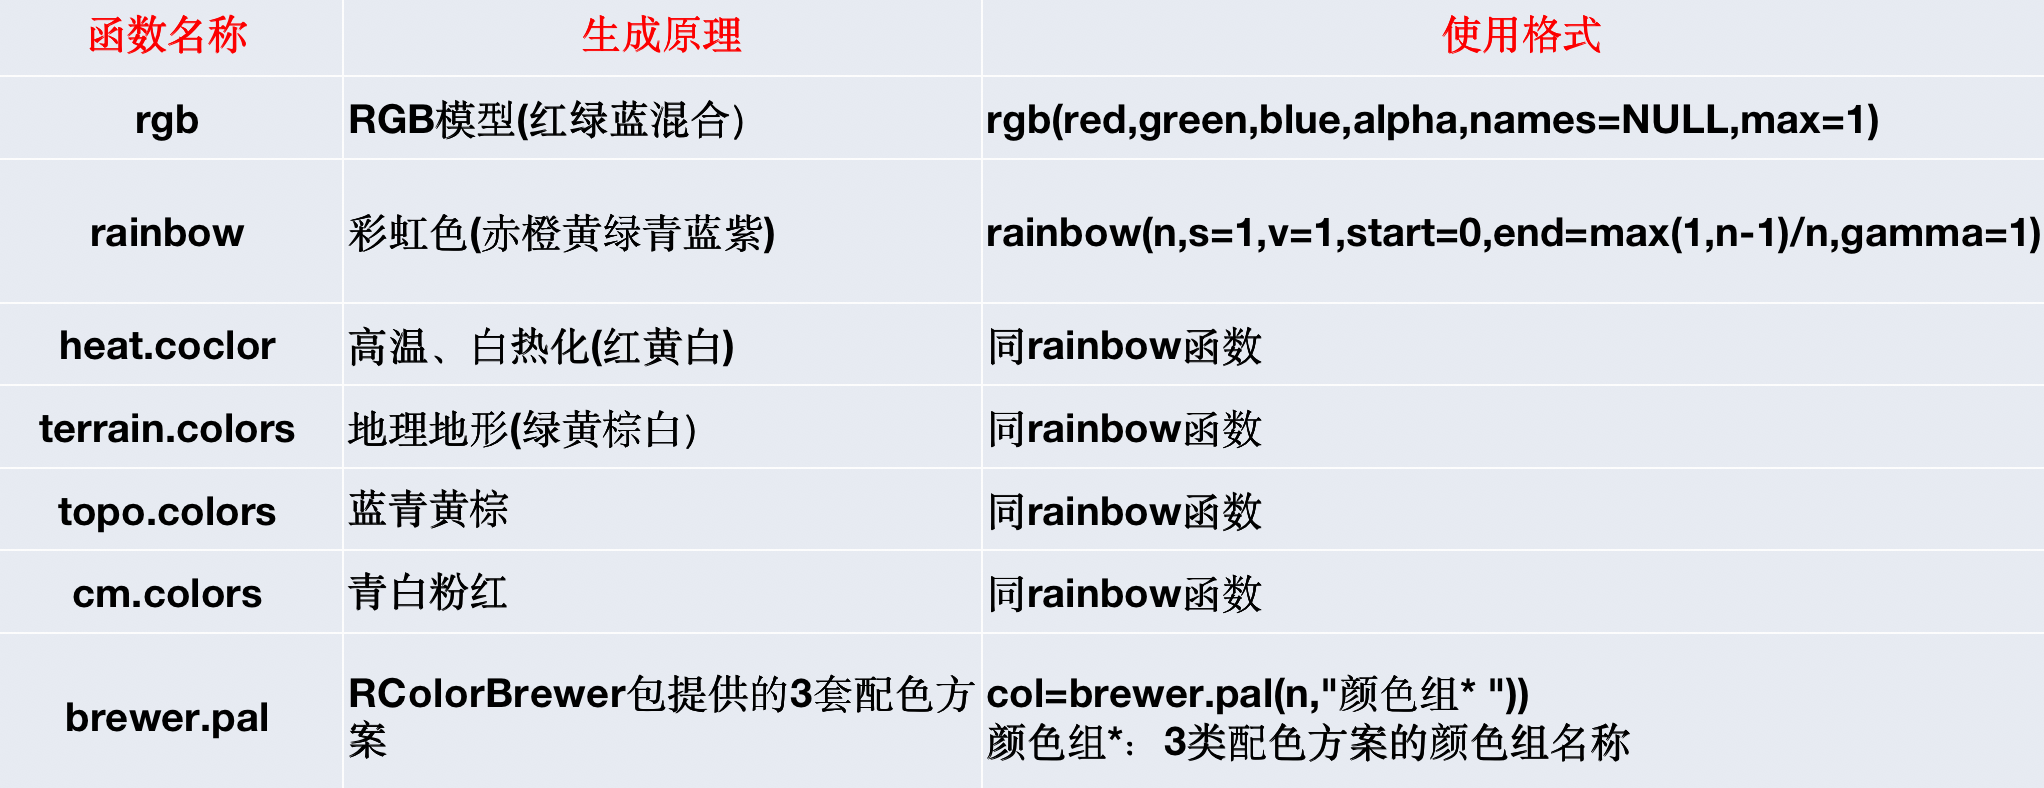
\includegraphics{figure/14.png}

rgb函数把RGB颜色转化为十六进制数值,使用格式前四个参数都取值于区间{[}0, max{]},names参数用来指定生成颜色向量的名称。red,green,blue参数的值越大就说明该颜色的成分越高。alpha指的是颜色的透明度,取0表示完全透明,取最大值表示完全不透明(默认完全不透明)。

\texttt{rainbow}函数、\texttt{heat.coclor}函数、\texttt{terrain.colors}函数、\texttt{topo.colors}函数、\texttt{cm.colors}函数是主题配色函数,使用格式中n设定产生颜色的数目,start和end设定彩虹颜色的一个子集,生成的颜色将从这个子集中选取。

\begin{center}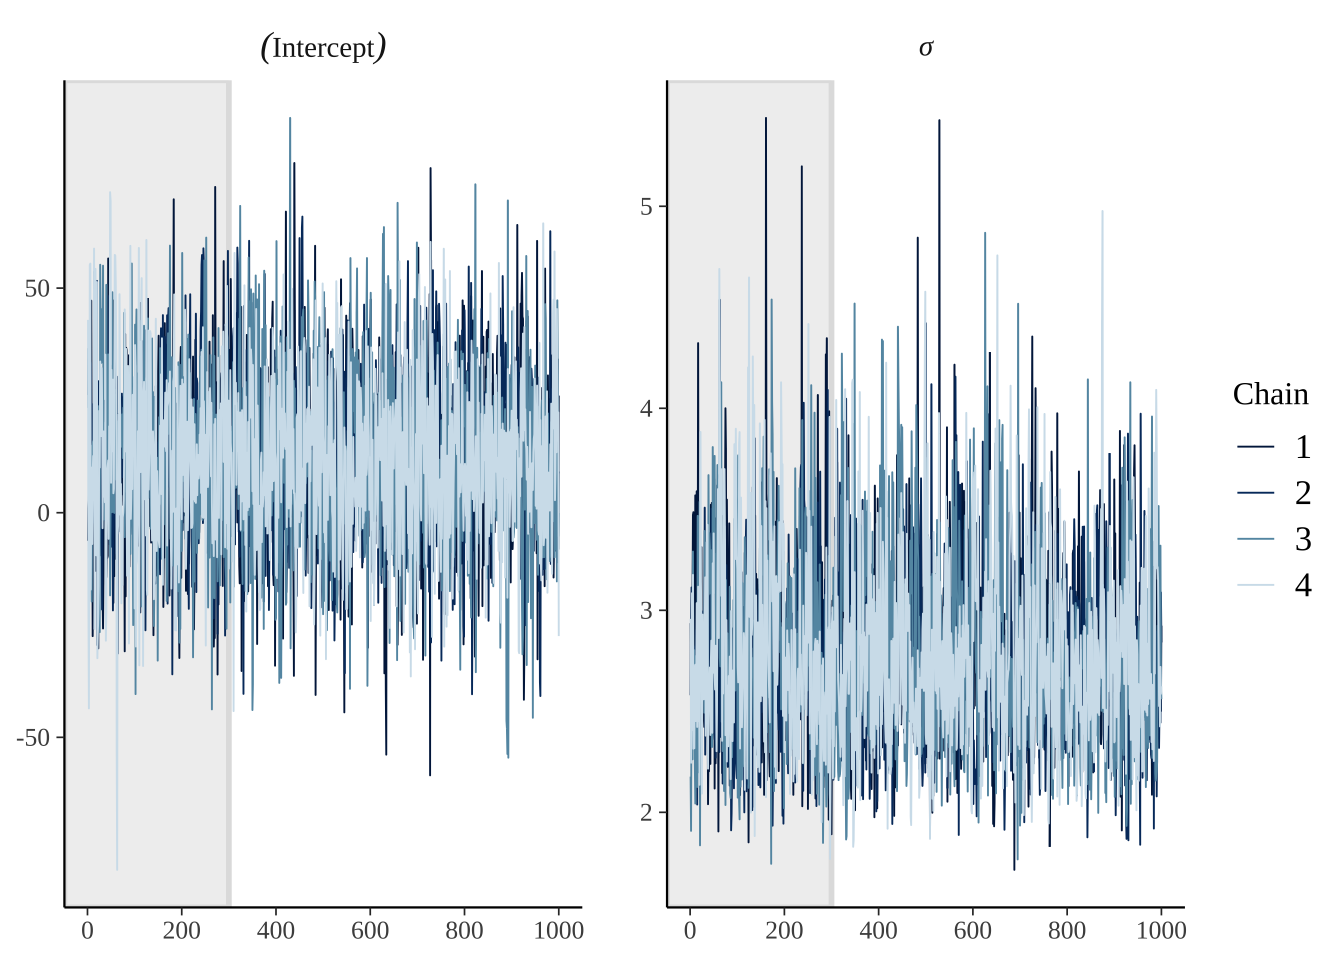
\includegraphics{1001-base-ploting_files/figure-latex/unnamed-chunk-24-1} \end{center}

\hypertarget{rcolorbrewerux5305}{%
\subsubsection{RColorBrewer包}\label{rcolorbrewerux5305}}

RColorBrewer包提供了3套配色方案,分别为\textbf{连续型,极端型以及离散型}。

\begin{itemize}
\item
  \textbf{连续型}(Sequential)指生成一系列连续渐变的颜色,通常用来标记连续型数值的大小。共18组颜色,每组分为9个渐变颜色展示。
\item
  \textbf{极端型}(Diverging)指生成用深色强调两端、浅色标示中部的系列颜色、可用来标记数据中的离群点。共9组颜色,每组分为11个渐变颜色展示。
\item
  \textbf{离散型}(Qualitative)指生成一系列彼此差异比较明显的颜色,通常用来标记分类数据。共8组颜色,每组渐变颜色数不同。
\end{itemize}

\begin{Shaded}
\begin{Highlighting}[]
\FunctionTok{par}\NormalTok{(}\AttributeTok{mfrow =} \FunctionTok{c}\NormalTok{(}\DecValTok{1}\NormalTok{,}\DecValTok{3}\NormalTok{))}
\FunctionTok{library}\NormalTok{(RColorBrewer)}
\FunctionTok{par}\NormalTok{(}\AttributeTok{mar=}\FunctionTok{c}\NormalTok{(}\FloatTok{0.1}\NormalTok{,}\DecValTok{3}\NormalTok{,}\FloatTok{0.1}\NormalTok{,}\FloatTok{0.1}\NormalTok{))}
\FunctionTok{display.brewer.all}\NormalTok{(}\AttributeTok{type=}\StringTok{"seq"}\NormalTok{)}
\FunctionTok{display.brewer.all}\NormalTok{(}\AttributeTok{type=}\StringTok{"div"}\NormalTok{)}
\FunctionTok{display.brewer.all}\NormalTok{(}\AttributeTok{type=}\StringTok{"qual"}\NormalTok{)}
\end{Highlighting}
\end{Shaded}

\begin{center}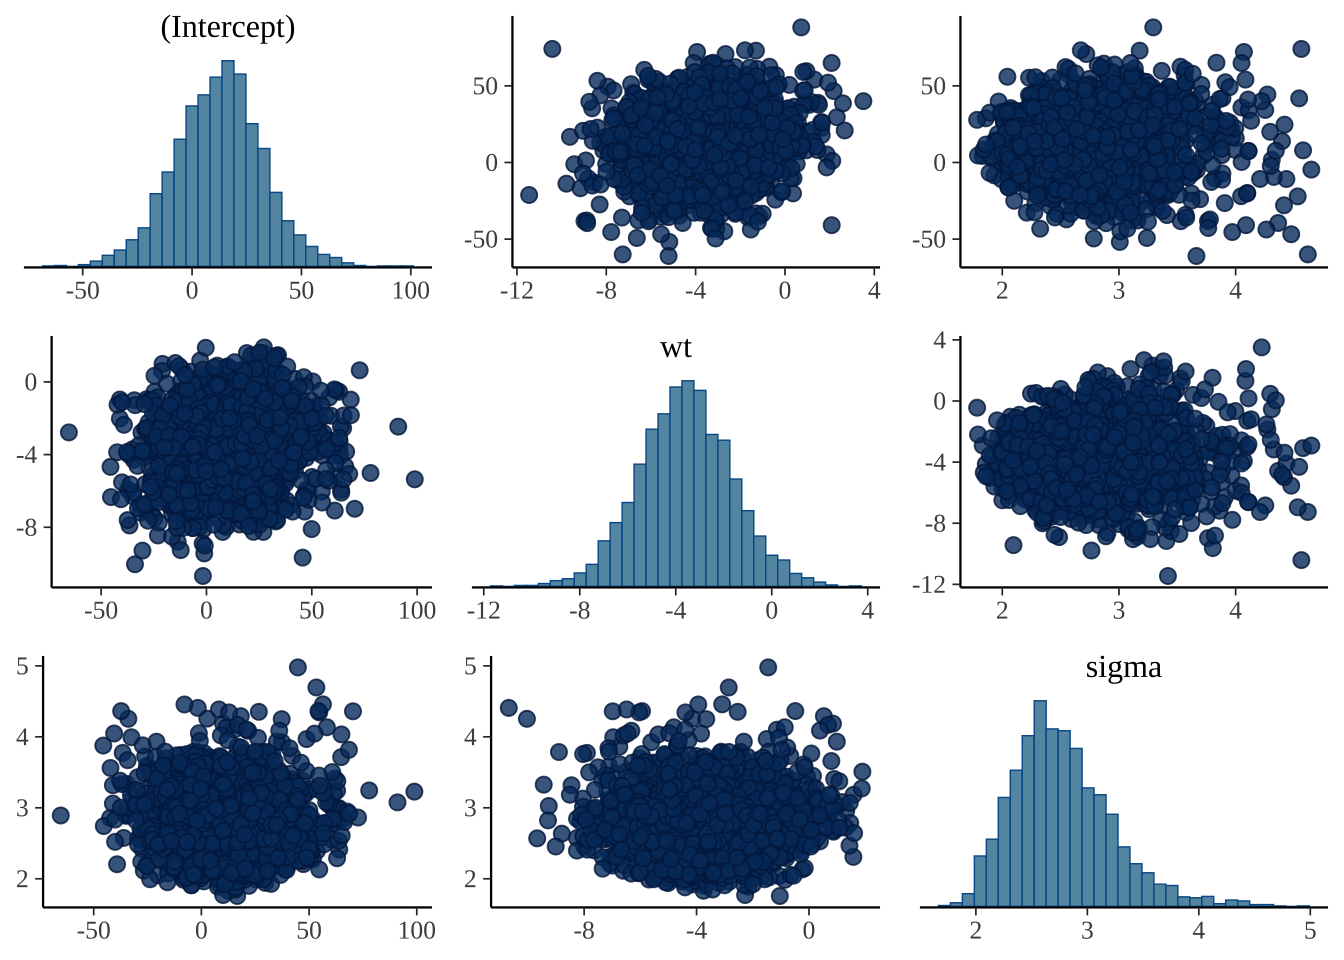
\includegraphics{1001-base-ploting_files/figure-latex/unnamed-chunk-25-1} \end{center}

\begin{Shaded}
\begin{Highlighting}[]
\FunctionTok{library}\NormalTok{(RColorBrewer)}
\NormalTok{my\_col }\OtherTok{\textless{}{-}} \FunctionTok{brewer.pal}\NormalTok{(}\DecValTok{3}\NormalTok{, }\StringTok{\textquotesingle{}RdYlGn\textquotesingle{}}\NormalTok{) }
\CommentTok{\# brewer.pal(n,name),其中n为颜色的数量,name表示颜色组的名称}
\FunctionTok{plot}\NormalTok{(iris}\SpecialCharTok{$}\NormalTok{Sepal.Length, iris}\SpecialCharTok{$}\NormalTok{Sepal.Width, }\AttributeTok{col =} \FunctionTok{rep}\NormalTok{(my\_col, }\AttributeTok{each =}\DecValTok{50}\NormalTok{))}
\end{Highlighting}
\end{Shaded}

\begin{center}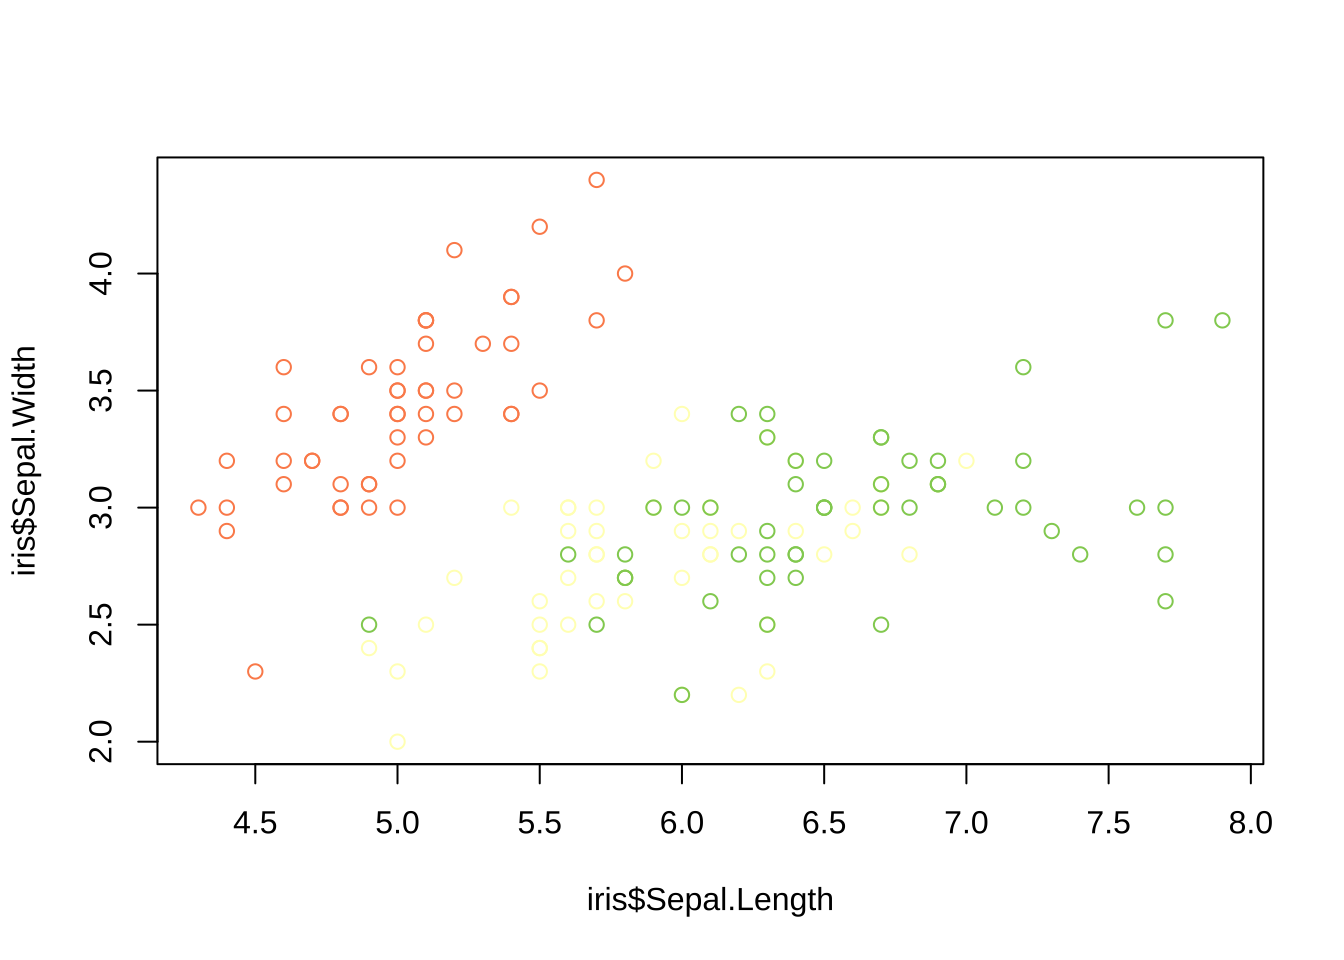
\includegraphics{1001-base-ploting_files/figure-latex/unnamed-chunk-26-1} \end{center}

\begin{Shaded}
\begin{Highlighting}[]
\FunctionTok{plot}\NormalTok{(iris}\SpecialCharTok{$}\NormalTok{Sepal.Length, iris}\SpecialCharTok{$}\NormalTok{Sepal.Width, }\AttributeTok{col =} \FunctionTok{rep}\NormalTok{(}\FunctionTok{rainbow}\NormalTok{(}\DecValTok{3}\NormalTok{), }\AttributeTok{each =} \DecValTok{50}\NormalTok{))}
\end{Highlighting}
\end{Shaded}

\begin{center}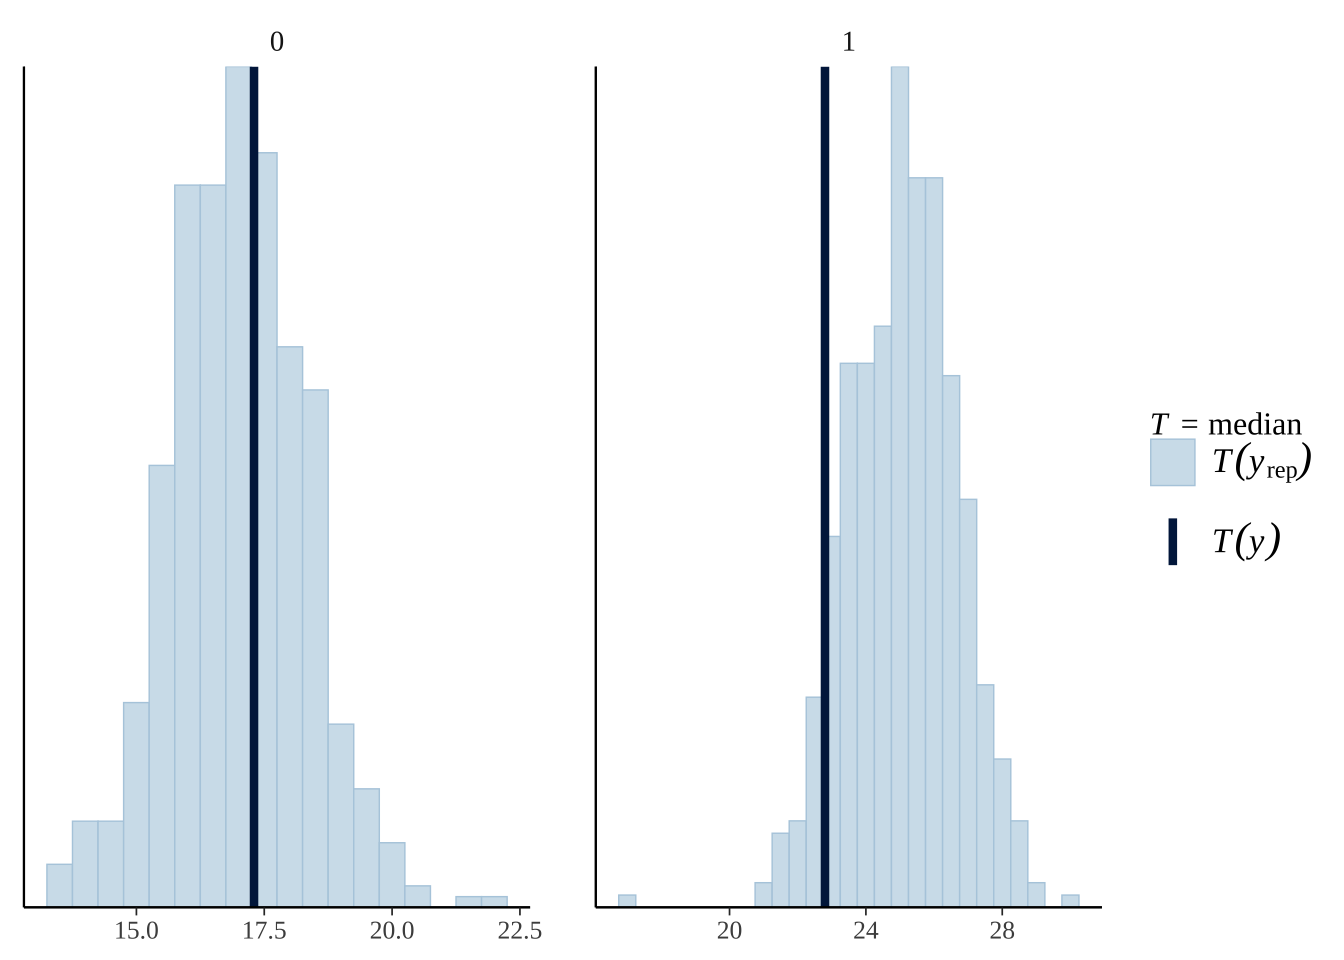
\includegraphics{1001-base-ploting_files/figure-latex/unnamed-chunk-26-2} \end{center}

\hypertarget{ux4feeux6539ux70b9ux7b26ux53f7ux4e0eux7ebfux6761}{%
\subsection{修改点符号与线条}\label{ux4feeux6539ux70b9ux7b26ux53f7ux4e0eux7ebfux6761}}

\hypertarget{ux70b9ux6837ux5f0f}{%
\subsubsection{点样式}\label{ux70b9ux6837ux5f0f}}

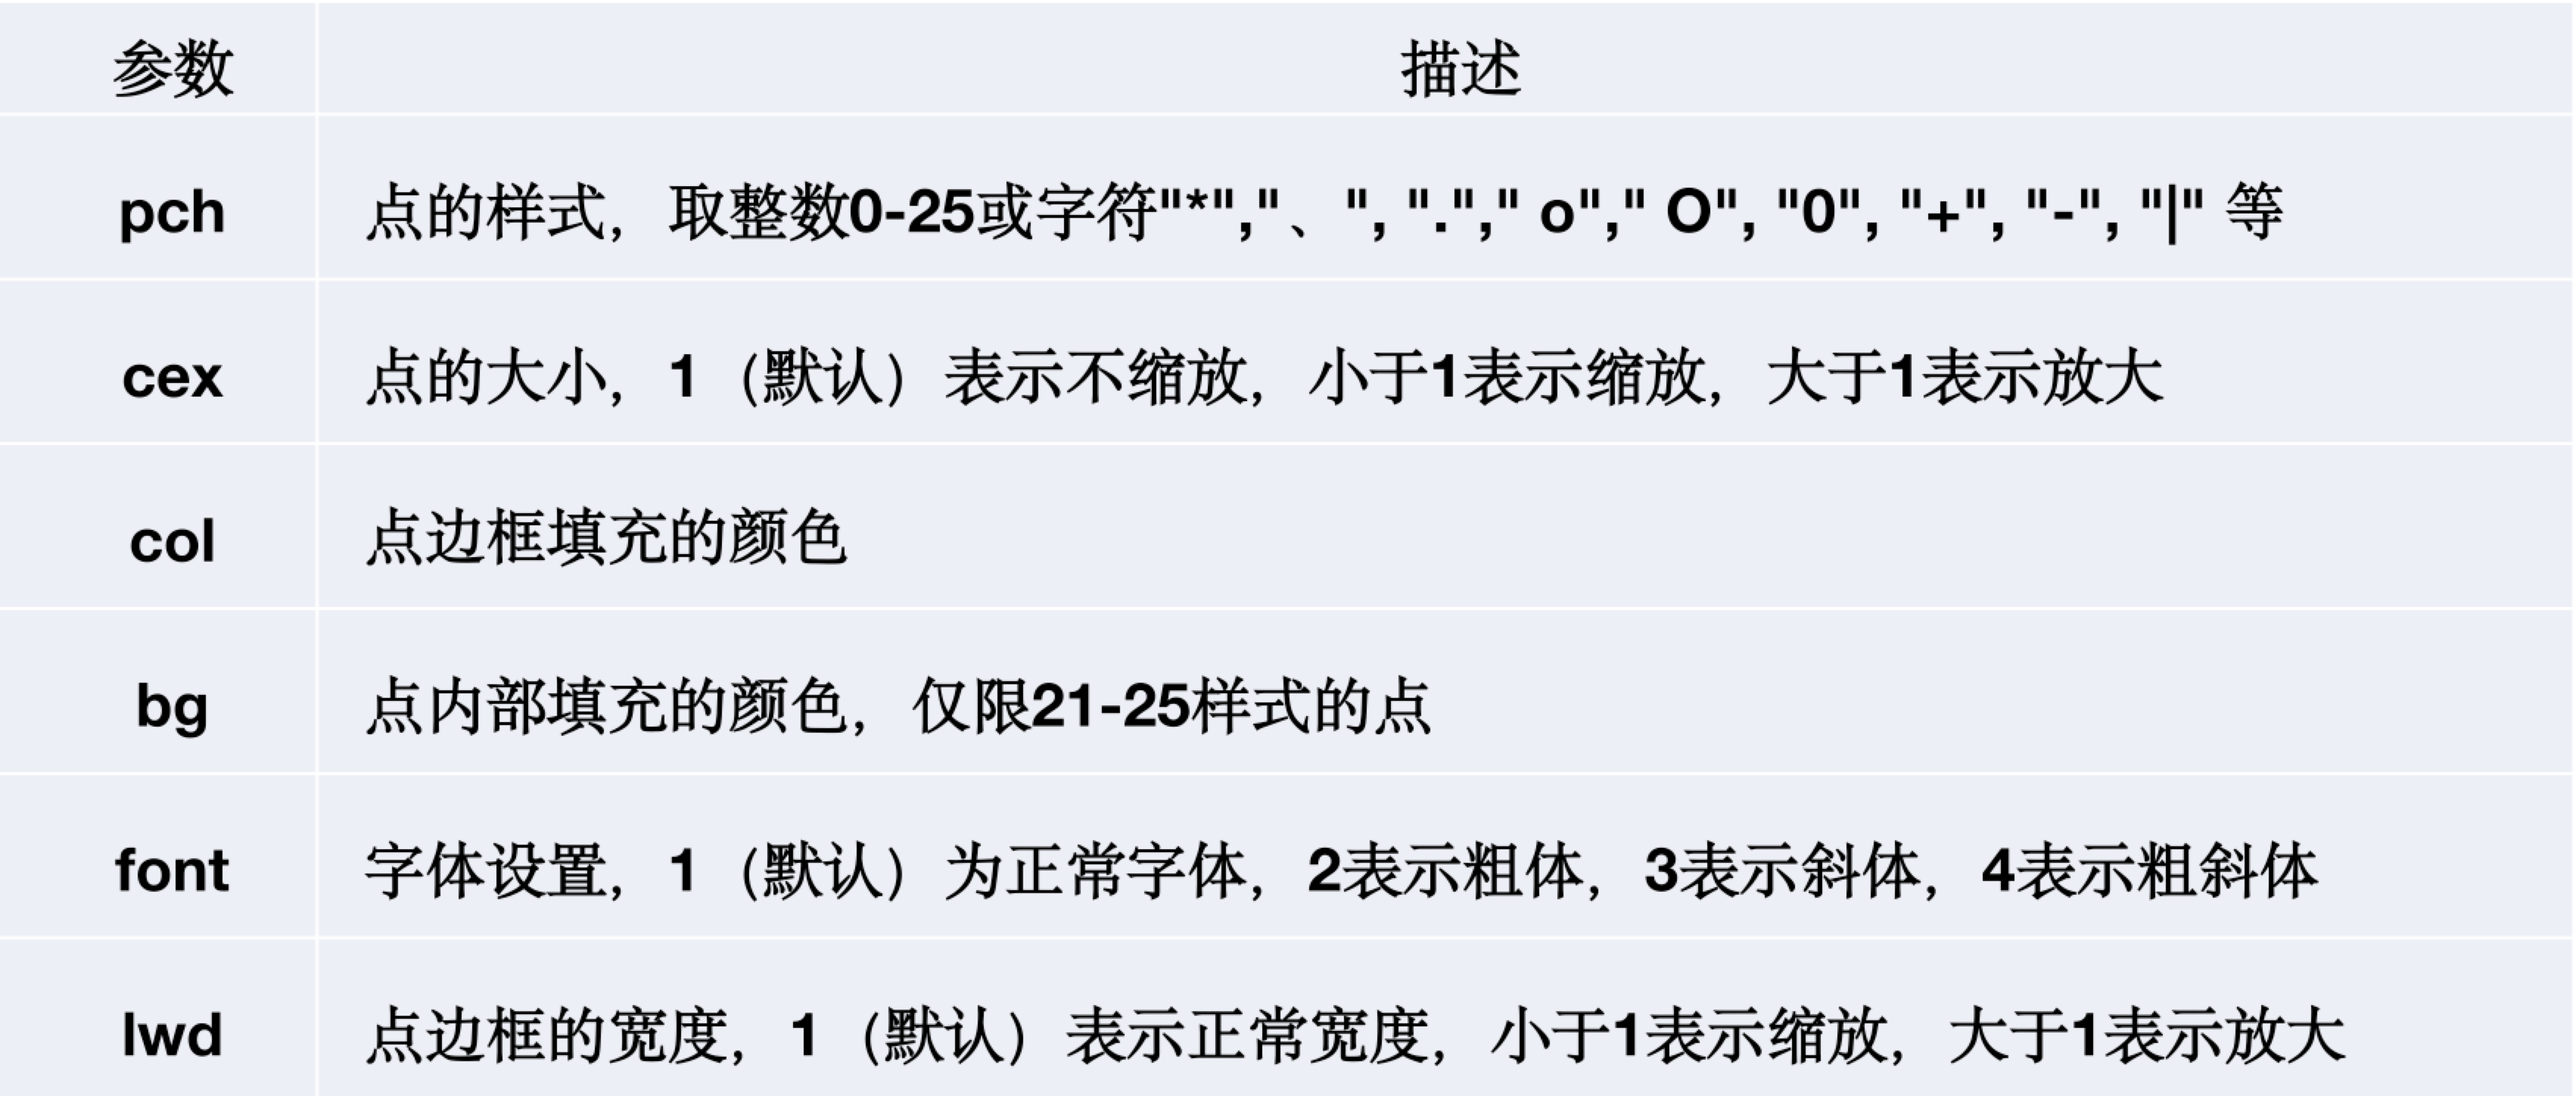
\includegraphics{figure/5.jpg}

\begin{center}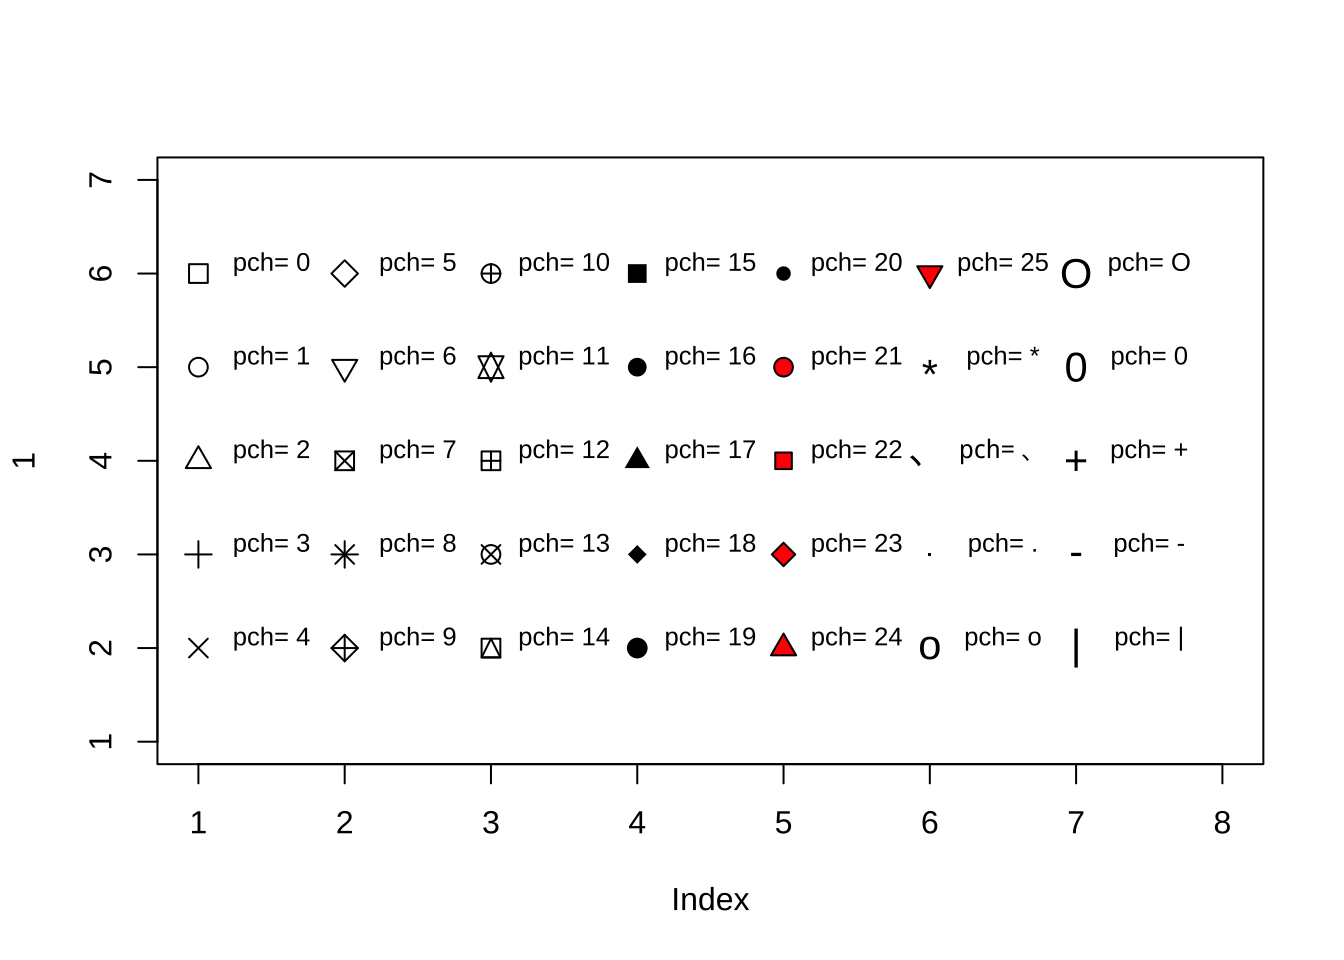
\includegraphics{1001-base-ploting_files/figure-latex/unnamed-chunk-27-1} \end{center}

\begin{Shaded}
\begin{Highlighting}[]
\FunctionTok{plot}\NormalTok{(iris}\SpecialCharTok{$}\NormalTok{Sepal.Length, iris}\SpecialCharTok{$}\NormalTok{Sepal.Width, }\AttributeTok{pch =} \FunctionTok{rep}\NormalTok{(}\DecValTok{1}\SpecialCharTok{:}\DecValTok{3}\NormalTok{, }\AttributeTok{each =} \DecValTok{50}\NormalTok{))}
\end{Highlighting}
\end{Shaded}

\begin{center}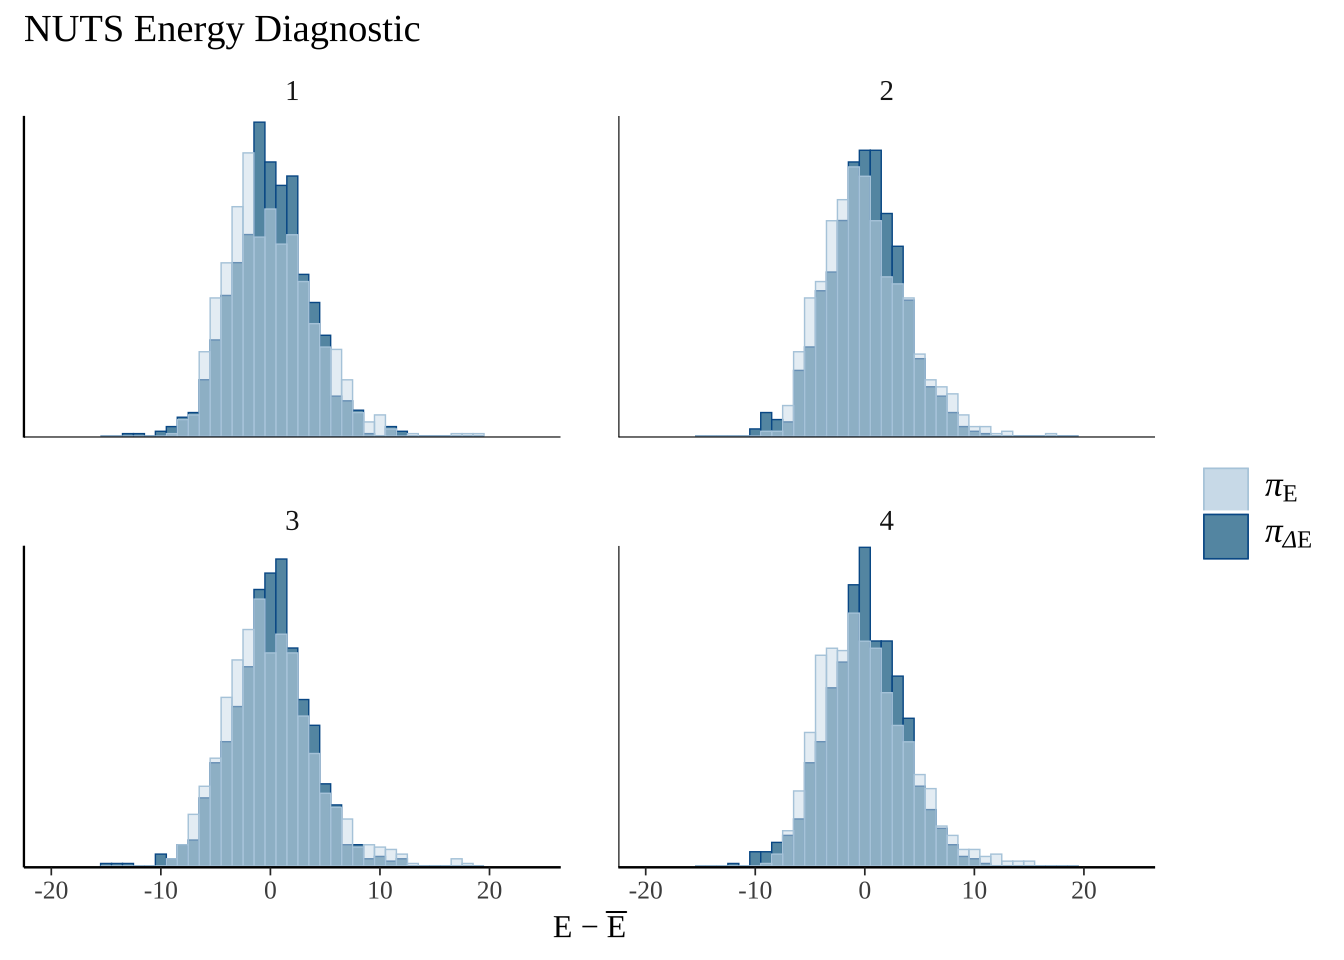
\includegraphics{1001-base-ploting_files/figure-latex/unnamed-chunk-28-1} \end{center}

\begin{Shaded}
\begin{Highlighting}[]
\CommentTok{\# plot(1:10,pch=21,cex=1.5,col=\textquotesingle{}red\textquotesingle{},bg = "blue",lwd=5)}
\end{Highlighting}
\end{Shaded}

\hypertarget{ux7ebfux6761ux6837ux5f0f}{%
\subsubsection{线条样式}\label{ux7ebfux6761ux6837ux5f0f}}

R语言提供了绘制不同类别的线条的多种函数,主要有

\begin{itemize}
\tightlist
\item
  lines:绘制曲线
\item
  abline:绘制直线
\item
  segments:绘制线段
\item
  arrows:在线段加上箭头
\item
  grid:绘制网格线
\end{itemize}

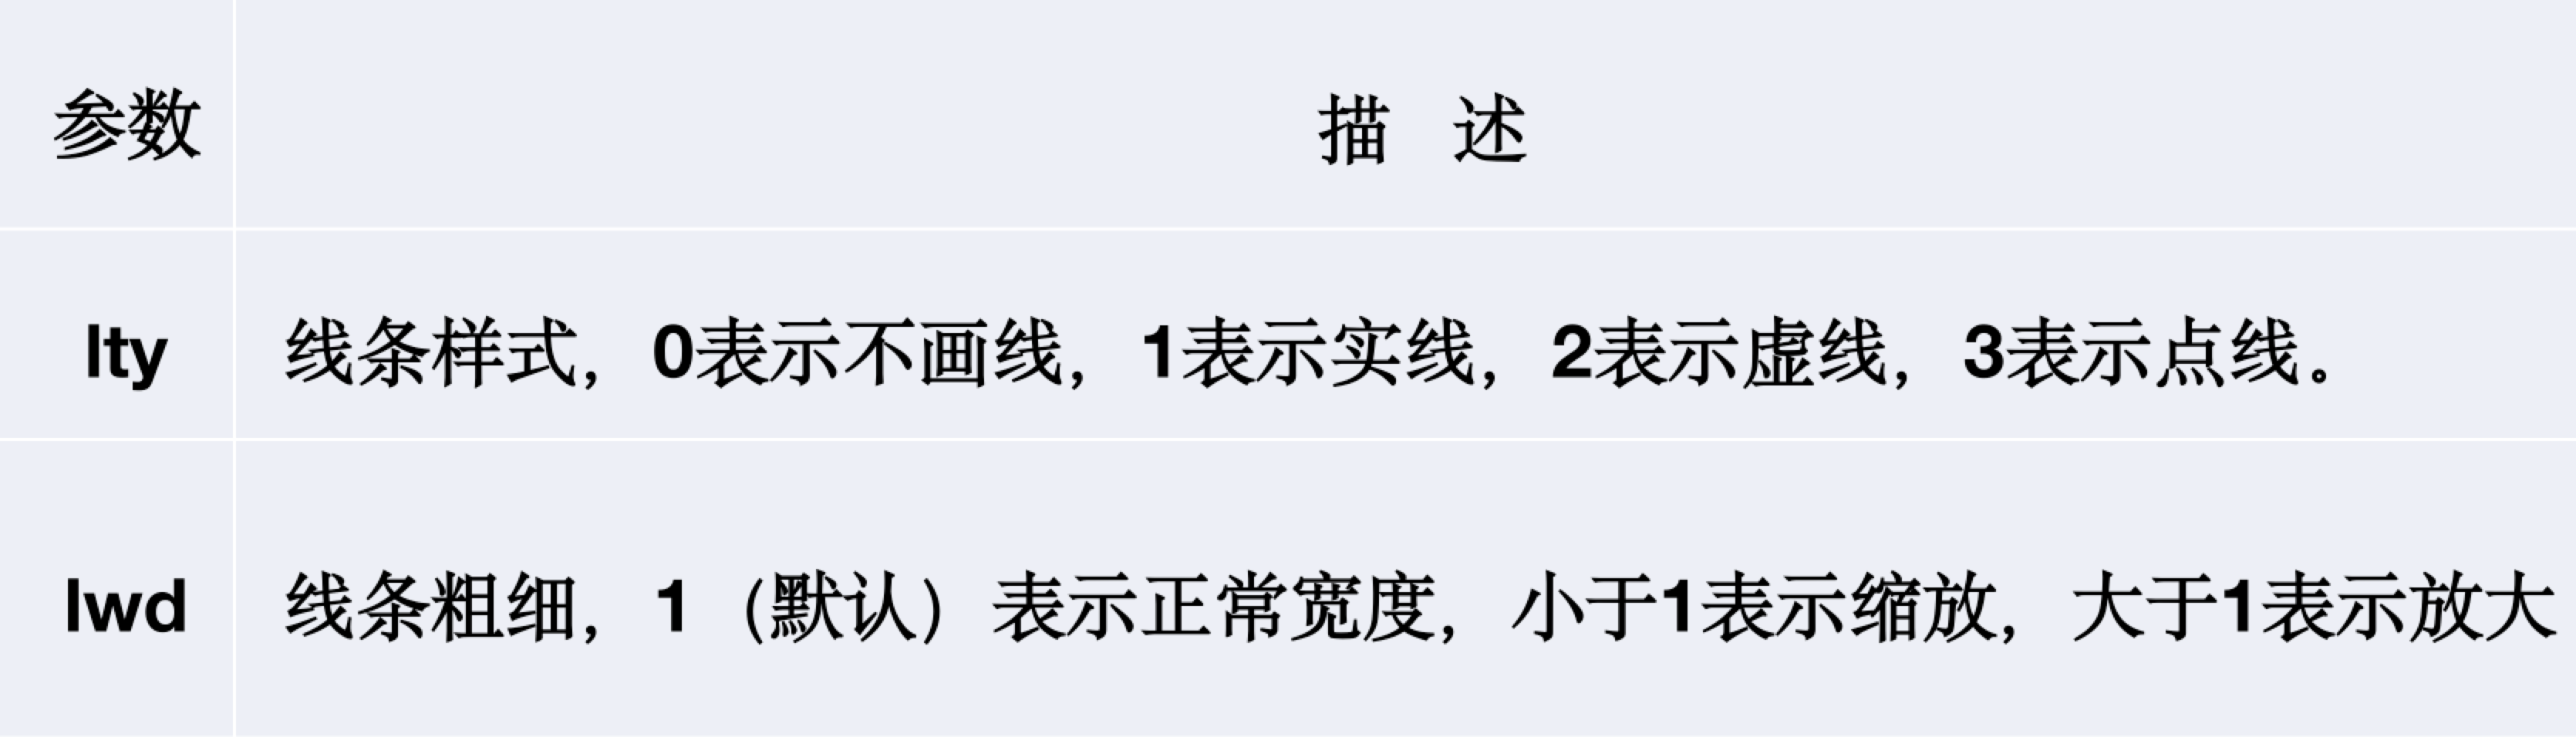
\includegraphics{figure/6.jpg}

以mtcars数据集为例来展示实际绘图过程中线条的应用。

\begin{Shaded}
\begin{Highlighting}[]
\FunctionTok{attach}\NormalTok{(mtcars)}
\NormalTok{smpg}\OtherTok{=}\NormalTok{(mpg}\SpecialCharTok{{-}}\FunctionTok{min}\NormalTok{(mpg))}\SpecialCharTok{/}\NormalTok{(}\FunctionTok{max}\NormalTok{(mpg)}\SpecialCharTok{{-}}\FunctionTok{min}\NormalTok{(mpg))}
\FunctionTok{plot}\NormalTok{(wt,smpg,}\AttributeTok{ylab=}\StringTok{"standardized mpg"}\NormalTok{)}
\CommentTok{\#添加核密度曲线图}
\FunctionTok{lines}\NormalTok{(}\FunctionTok{density}\NormalTok{(wt),}\AttributeTok{col=}\StringTok{"red"}\NormalTok{)}
\CommentTok{\#指向密度曲线的箭头}
\FunctionTok{arrows}\NormalTok{(}\FloatTok{1.8}\NormalTok{,}\FloatTok{0.05}\NormalTok{,}\FloatTok{1.5}\NormalTok{,}\FloatTok{0.1}\NormalTok{)}
\FunctionTok{text}\NormalTok{(}\DecValTok{2}\NormalTok{,}\FloatTok{0.05}\NormalTok{,}\StringTok{"density curve"}\NormalTok{,}\AttributeTok{cex=}\FloatTok{0.6}\NormalTok{)}
\CommentTok{\#添加回归线}
\FunctionTok{abline}\NormalTok{(}\FunctionTok{lm}\NormalTok{(smpg}\SpecialCharTok{\textasciitilde{}}\NormalTok{wt),}\AttributeTok{lty=}\DecValTok{2}\NormalTok{,}\AttributeTok{col=}\StringTok{"green"}\NormalTok{)}
\CommentTok{\#指向回归直线的箭头}
\FunctionTok{arrows}\NormalTok{(}\DecValTok{2}\NormalTok{,}\FloatTok{0.5}\NormalTok{,}\DecValTok{2}\NormalTok{,}\FloatTok{0.7}\NormalTok{,}\AttributeTok{angle=}\DecValTok{10}\NormalTok{,}\AttributeTok{cex=}\FloatTok{0.5}\NormalTok{)}
\FunctionTok{text}\NormalTok{(}\DecValTok{2}\NormalTok{,}\FloatTok{0.45}\NormalTok{,}\StringTok{"regression line"}\NormalTok{,}\AttributeTok{cex=}\FloatTok{0.6}\NormalTok{)}
\CommentTok{\#wt与mpg反向线性相关,添加最大最小值线段表现这种关系}
\FunctionTok{segments}\NormalTok{(}\FunctionTok{min}\NormalTok{(wt),}\FunctionTok{max}\NormalTok{(smpg),}\FunctionTok{max}\NormalTok{(wt),}\FunctionTok{min}\NormalTok{(smpg),}\AttributeTok{lty=}\DecValTok{3}\NormalTok{,}\AttributeTok{col=}\StringTok{"blue"}\NormalTok{)}
\CommentTok{\#指向最大最小值线段的箭头}
\FunctionTok{arrows}\NormalTok{(}\DecValTok{3}\NormalTok{,}\FloatTok{0.8}\NormalTok{,}\FloatTok{2.5}\NormalTok{,}\FloatTok{0.76}\NormalTok{,}\AttributeTok{angle=}\DecValTok{10}\NormalTok{,}\AttributeTok{cex=}\FloatTok{0.5}\NormalTok{)}
\FunctionTok{text}\NormalTok{(}\FloatTok{3.3}\NormalTok{,}\FloatTok{0.8}\NormalTok{,}\StringTok{"line segments"}\NormalTok{,}\AttributeTok{cex=}\FloatTok{0.6}\NormalTok{)}
\CommentTok{\#添加网格线作为背景}
\FunctionTok{grid}\NormalTok{(}\AttributeTok{nx=}\DecValTok{4}\NormalTok{,}\AttributeTok{ny=}\DecValTok{5}\NormalTok{,}\AttributeTok{lty=}\DecValTok{2}\NormalTok{,}\AttributeTok{col=}\StringTok{"grey"}\NormalTok{)}
\end{Highlighting}
\end{Shaded}

\begin{center}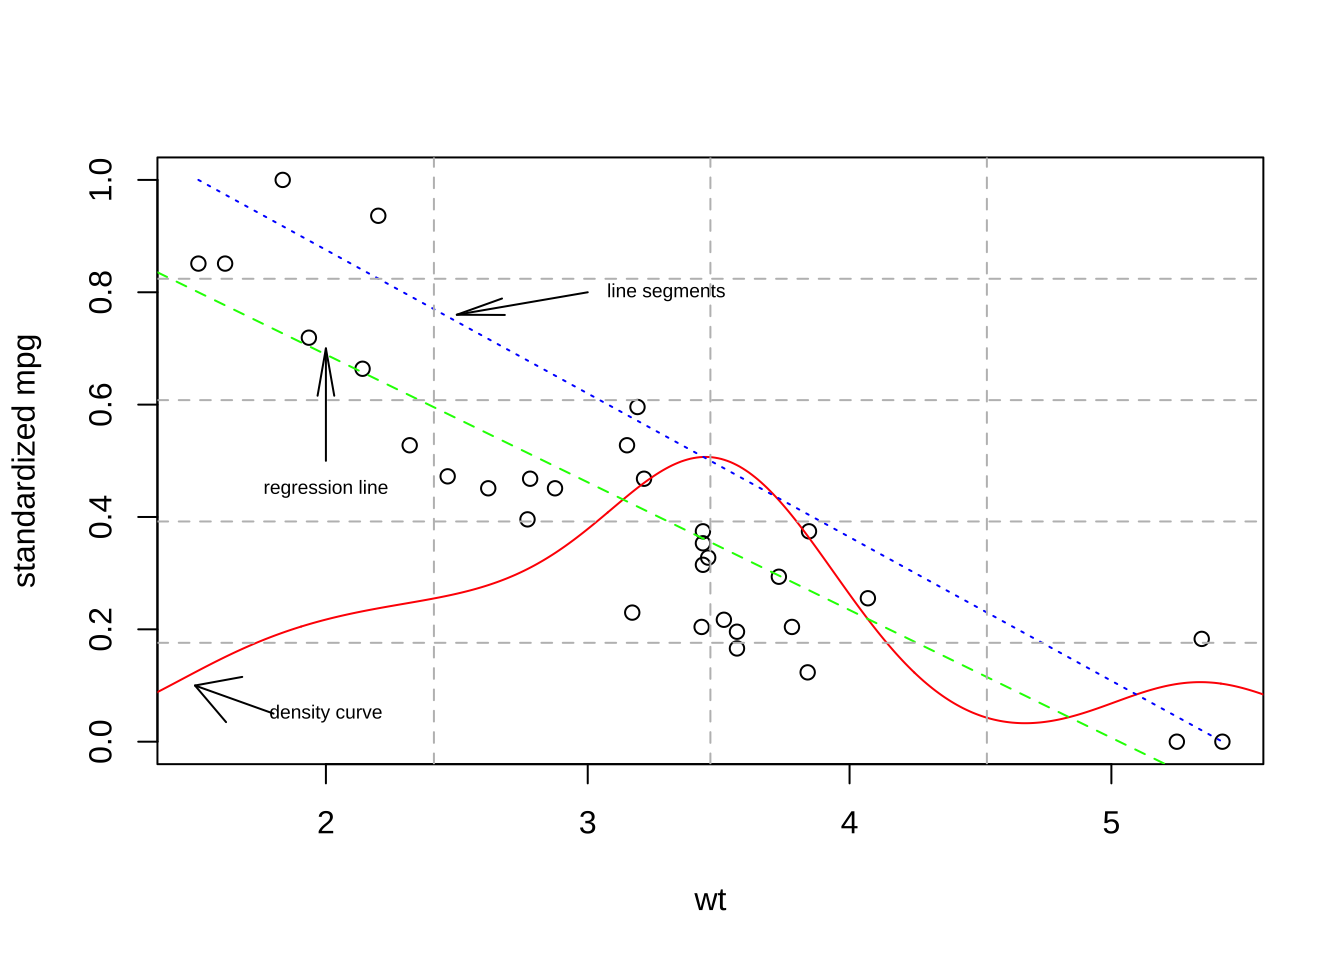
\includegraphics{1001-base-ploting_files/figure-latex/unnamed-chunk-29-1} \end{center}

\hypertarget{ux4feeux6539ux6587ux672cux53c2ux6570}{%
\subsubsection{修改文本参数}\label{ux4feeux6539ux6587ux672cux53c2ux6570}}

title、text和mtext函数可以在打开的画布上添加文字元素。

\begin{itemize}
\tightlist
\item
  title可以添加标题元素;
\item
  text可以任意位置添加文本;
\item
  mtext函数则是在四条边上添加文本。
\end{itemize}

\begin{Shaded}
\begin{Highlighting}[]
\FunctionTok{par}\NormalTok{(}\AttributeTok{mfrow =} \FunctionTok{c}\NormalTok{(}\DecValTok{2}\NormalTok{, }\DecValTok{2}\NormalTok{))}
\CommentTok{\# 图一:图形添加标题}
\FunctionTok{plot}\NormalTok{(}\FunctionTok{c}\NormalTok{(}\DecValTok{0}\SpecialCharTok{:}\DecValTok{5}\NormalTok{),}\AttributeTok{col=}\StringTok{"red"}\NormalTok{,}\AttributeTok{xlab=}\StringTok{""}\NormalTok{,}\AttributeTok{ylab=}\StringTok{""}\NormalTok{)}
\FunctionTok{title}\NormalTok{(}\AttributeTok{main=}\FunctionTok{list}\NormalTok{(}\StringTok{"主标题"}\NormalTok{,}\AttributeTok{cex=}\FloatTok{1.5}\NormalTok{),}\AttributeTok{sub=}\FunctionTok{list}\NormalTok{(}\StringTok{"副标题"}\NormalTok{,}\AttributeTok{cex=}\FloatTok{1.2}\NormalTok{), }
      \AttributeTok{xlab=}\StringTok{"x轴标题"}\NormalTok{,}\AttributeTok{ylab=}\StringTok{"y轴标题"}\NormalTok{)}
\CommentTok{\# 图二:图形周边添加文本}
\FunctionTok{plot}\NormalTok{(}\FunctionTok{c}\NormalTok{(}\DecValTok{0}\SpecialCharTok{:}\DecValTok{5}\NormalTok{),}\AttributeTok{col=}\StringTok{"white"}\NormalTok{)}
\FunctionTok{mtext}\NormalTok{(}\StringTok{\textquotesingle{}side=1:下边\textquotesingle{}}\NormalTok{,}\AttributeTok{side=}\DecValTok{1}\NormalTok{,}\AttributeTok{line=}\DecValTok{2}\NormalTok{)}
\FunctionTok{mtext}\NormalTok{(}\StringTok{\textquotesingle{}side=2:左边\textquotesingle{}}\NormalTok{ ,}\AttributeTok{side=}\DecValTok{2}\NormalTok{,}\AttributeTok{line=}\DecValTok{2}\NormalTok{)}
\FunctionTok{mtext}\NormalTok{(}\StringTok{\textquotesingle{}side=3:上边\textquotesingle{}}\NormalTok{ ,}\AttributeTok{side=}\DecValTok{3}\NormalTok{)}
\FunctionTok{mtext}\NormalTok{(}\StringTok{\textquotesingle{}side=4:右边\textquotesingle{}}\NormalTok{ ,}\AttributeTok{side=}\DecValTok{4}\NormalTok{)}
\CommentTok{\# 图三:字体展示}
\FunctionTok{plot}\NormalTok{(}\FunctionTok{c}\NormalTok{(}\DecValTok{0}\SpecialCharTok{:}\DecValTok{5}\NormalTok{),}\AttributeTok{col=}\StringTok{"white"}\NormalTok{)}
\FunctionTok{text}\NormalTok{(}\DecValTok{2}\NormalTok{,}\DecValTok{4}\NormalTok{,}\AttributeTok{labels=}\StringTok{"font=1:正常字体(默认)"}\NormalTok{,}\AttributeTok{font=}\DecValTok{1}\NormalTok{)}
\FunctionTok{text}\NormalTok{(}\DecValTok{3}\NormalTok{,}\DecValTok{3}\NormalTok{,}\AttributeTok{labels=}\StringTok{"font=2:粗体字体"}\NormalTok{,}\AttributeTok{font=}\DecValTok{2}\NormalTok{)}
\FunctionTok{text}\NormalTok{(}\DecValTok{4}\NormalTok{,}\DecValTok{2}\NormalTok{,}\AttributeTok{labels=}\StringTok{"font=3:斜体字体"}\NormalTok{,}\AttributeTok{font=}\DecValTok{3}\NormalTok{)}
\FunctionTok{text}\NormalTok{(}\DecValTok{5}\NormalTok{,}\DecValTok{1}\NormalTok{,}\AttributeTok{labels=}\StringTok{"font=4:粗斜体字体"}\NormalTok{,}\AttributeTok{font=}\DecValTok{4}\NormalTok{)}
\CommentTok{\# 图四:字体大小展示}
\FunctionTok{plot}\NormalTok{(}\FunctionTok{c}\NormalTok{(}\DecValTok{0}\SpecialCharTok{:}\DecValTok{6}\NormalTok{),}\AttributeTok{col=}\StringTok{"white"}\NormalTok{,}\AttributeTok{xlim=}\FunctionTok{c}\NormalTok{(}\DecValTok{1}\NormalTok{,}\DecValTok{8}\NormalTok{))}
\FunctionTok{text}\NormalTok{(}\DecValTok{2}\NormalTok{,}\DecValTok{5}\NormalTok{,}\AttributeTok{labels=}\StringTok{"cex=0.5:放大0.5倍"}\NormalTok{,}\AttributeTok{cex=}\FloatTok{0.5}\NormalTok{)}
\FunctionTok{text}\NormalTok{(}\DecValTok{3}\NormalTok{,}\DecValTok{4}\NormalTok{,}\AttributeTok{labels=}\StringTok{"cex=0.8:放大0.8倍"}\NormalTok{,}\AttributeTok{cex=}\FloatTok{0.8}\NormalTok{)}
\FunctionTok{text}\NormalTok{(}\DecValTok{4}\NormalTok{,}\DecValTok{3}\NormalTok{,}\AttributeTok{labels=}\StringTok{"cex=1(默认):正常大小"}\NormalTok{,}\AttributeTok{cex=}\DecValTok{1}\NormalTok{)}
\FunctionTok{text}\NormalTok{(}\DecValTok{5}\NormalTok{,}\DecValTok{2}\NormalTok{,}\AttributeTok{labels=}\StringTok{"cex=1.2:放大1.2倍"}\NormalTok{,}\AttributeTok{cex=}\FloatTok{1.2}\NormalTok{)}
\FunctionTok{text}\NormalTok{(}\DecValTok{6}\NormalTok{,}\DecValTok{1}\NormalTok{,}\AttributeTok{labels=}\StringTok{"cex=1.5:放大1.5倍"}\NormalTok{,}\AttributeTok{cex=}\FloatTok{1.5}\NormalTok{)}
\end{Highlighting}
\end{Shaded}

\begin{center}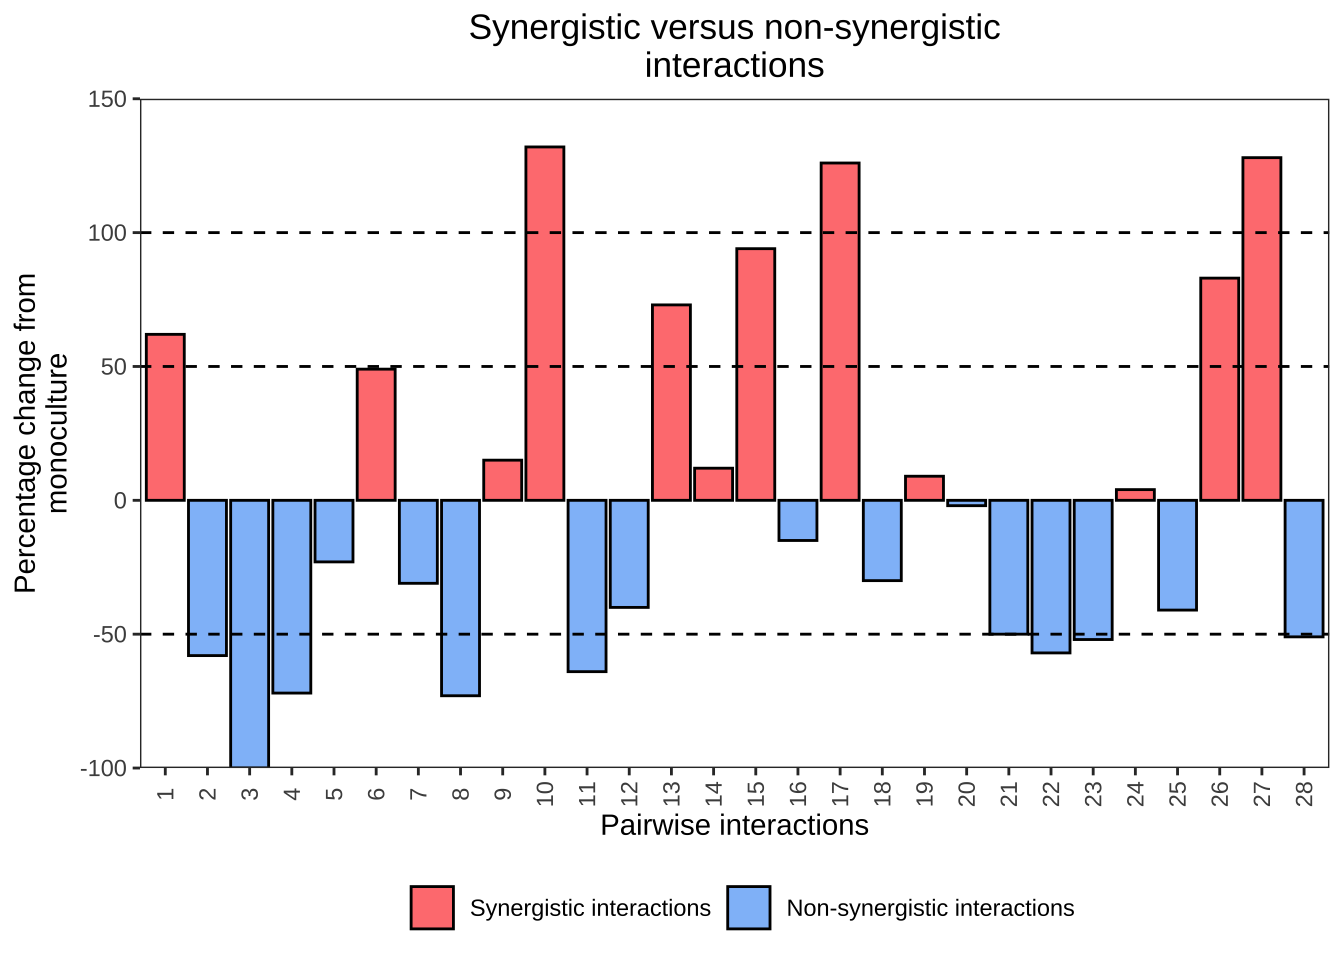
\includegraphics{1001-base-ploting_files/figure-latex/unnamed-chunk-30-1} \end{center}

\textbf{例子}:

\begin{Shaded}
\begin{Highlighting}[]
\FunctionTok{attach}\NormalTok{(mtcars)}
\FunctionTok{plot}\NormalTok{(wt, mpg, }\AttributeTok{xlab =} \StringTok{"Weight (1000 lbs)"}\NormalTok{, }
     \AttributeTok{ylab =} \StringTok{"Miles/(US) gallon"}\NormalTok{) }\CommentTok{\#绘图,并修改x,y轴的标题}
\FunctionTok{title}\NormalTok{(}\AttributeTok{main=}\FunctionTok{list}\NormalTok{(}\StringTok{"mtcars wt V.S. mpg"}\NormalTok{, }\AttributeTok{cex=}\FloatTok{1.5}\NormalTok{))  }\CommentTok{\# 添加标题}
\FunctionTok{text}\NormalTok{(}\FloatTok{4.5}\NormalTok{, }\DecValTok{34}\NormalTok{, }\AttributeTok{labels =} \StringTok{\textquotesingle{}extracted from the 1974\textquotesingle{}}\NormalTok{, }\AttributeTok{cex =} \FloatTok{1.5}\NormalTok{)  }\CommentTok{\# 说明数据来源}
\FunctionTok{text}\NormalTok{(}\FloatTok{4.5}\NormalTok{, }\DecValTok{32}\NormalTok{, }\AttributeTok{labels =} \StringTok{\textquotesingle{}Motor Trend US\textquotesingle{}}\NormalTok{, }\AttributeTok{font =} \DecValTok{3}\NormalTok{)  }\CommentTok{\# 杂志名称}
\end{Highlighting}
\end{Shaded}

\begin{center}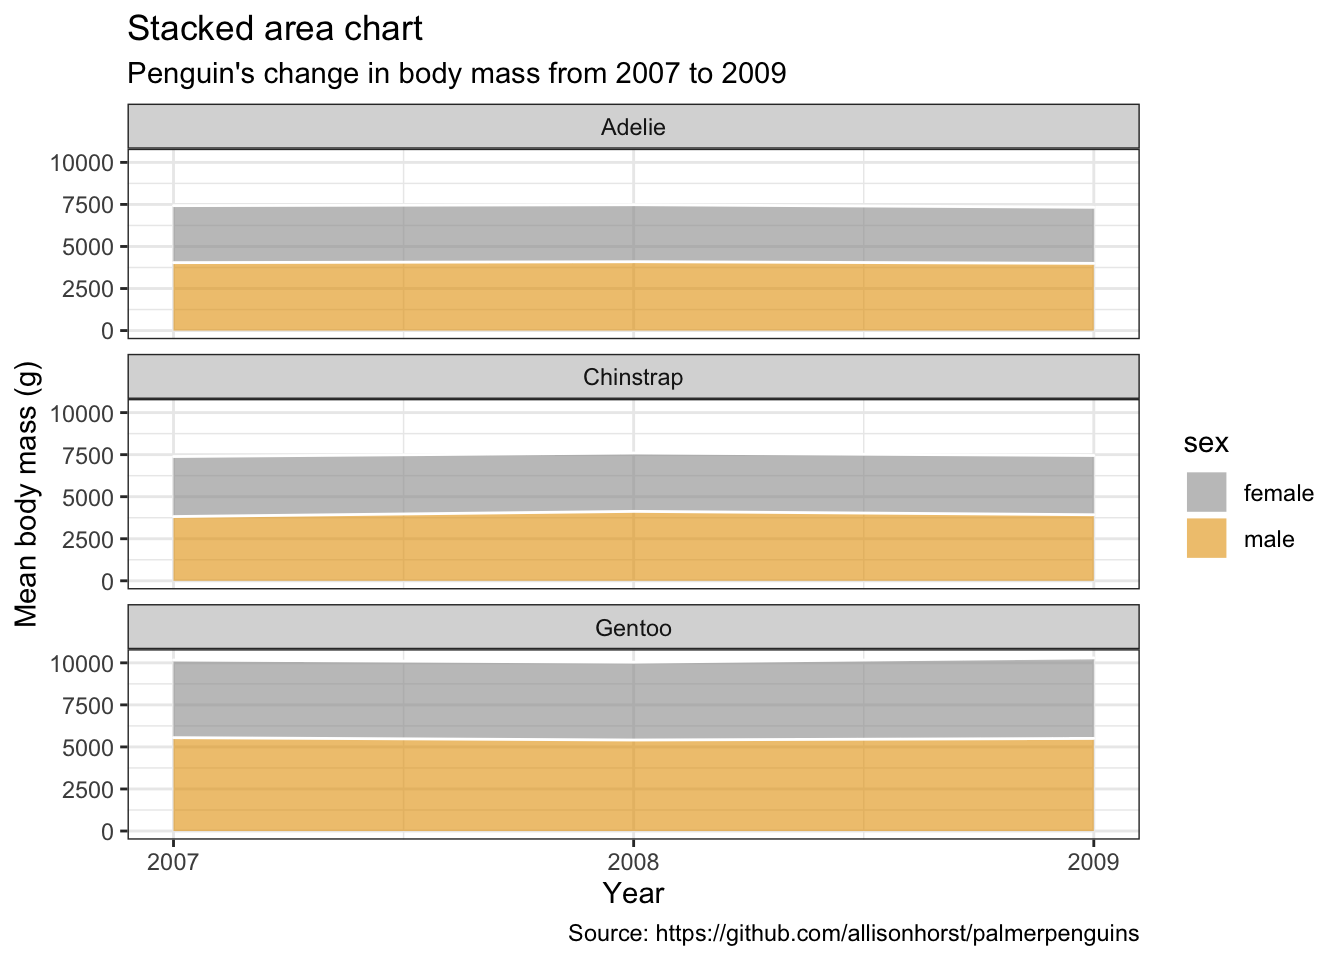
\includegraphics{1001-base-ploting_files/figure-latex/unnamed-chunk-31-1} \end{center}

\hypertarget{ux8bbeux7f6eux5750ux6807ux8f74}{%
\subsubsection{设置坐标轴}\label{ux8bbeux7f6eux5750ux6807ux8f74}}

使用\texttt{axis()}进行设置坐标轴。

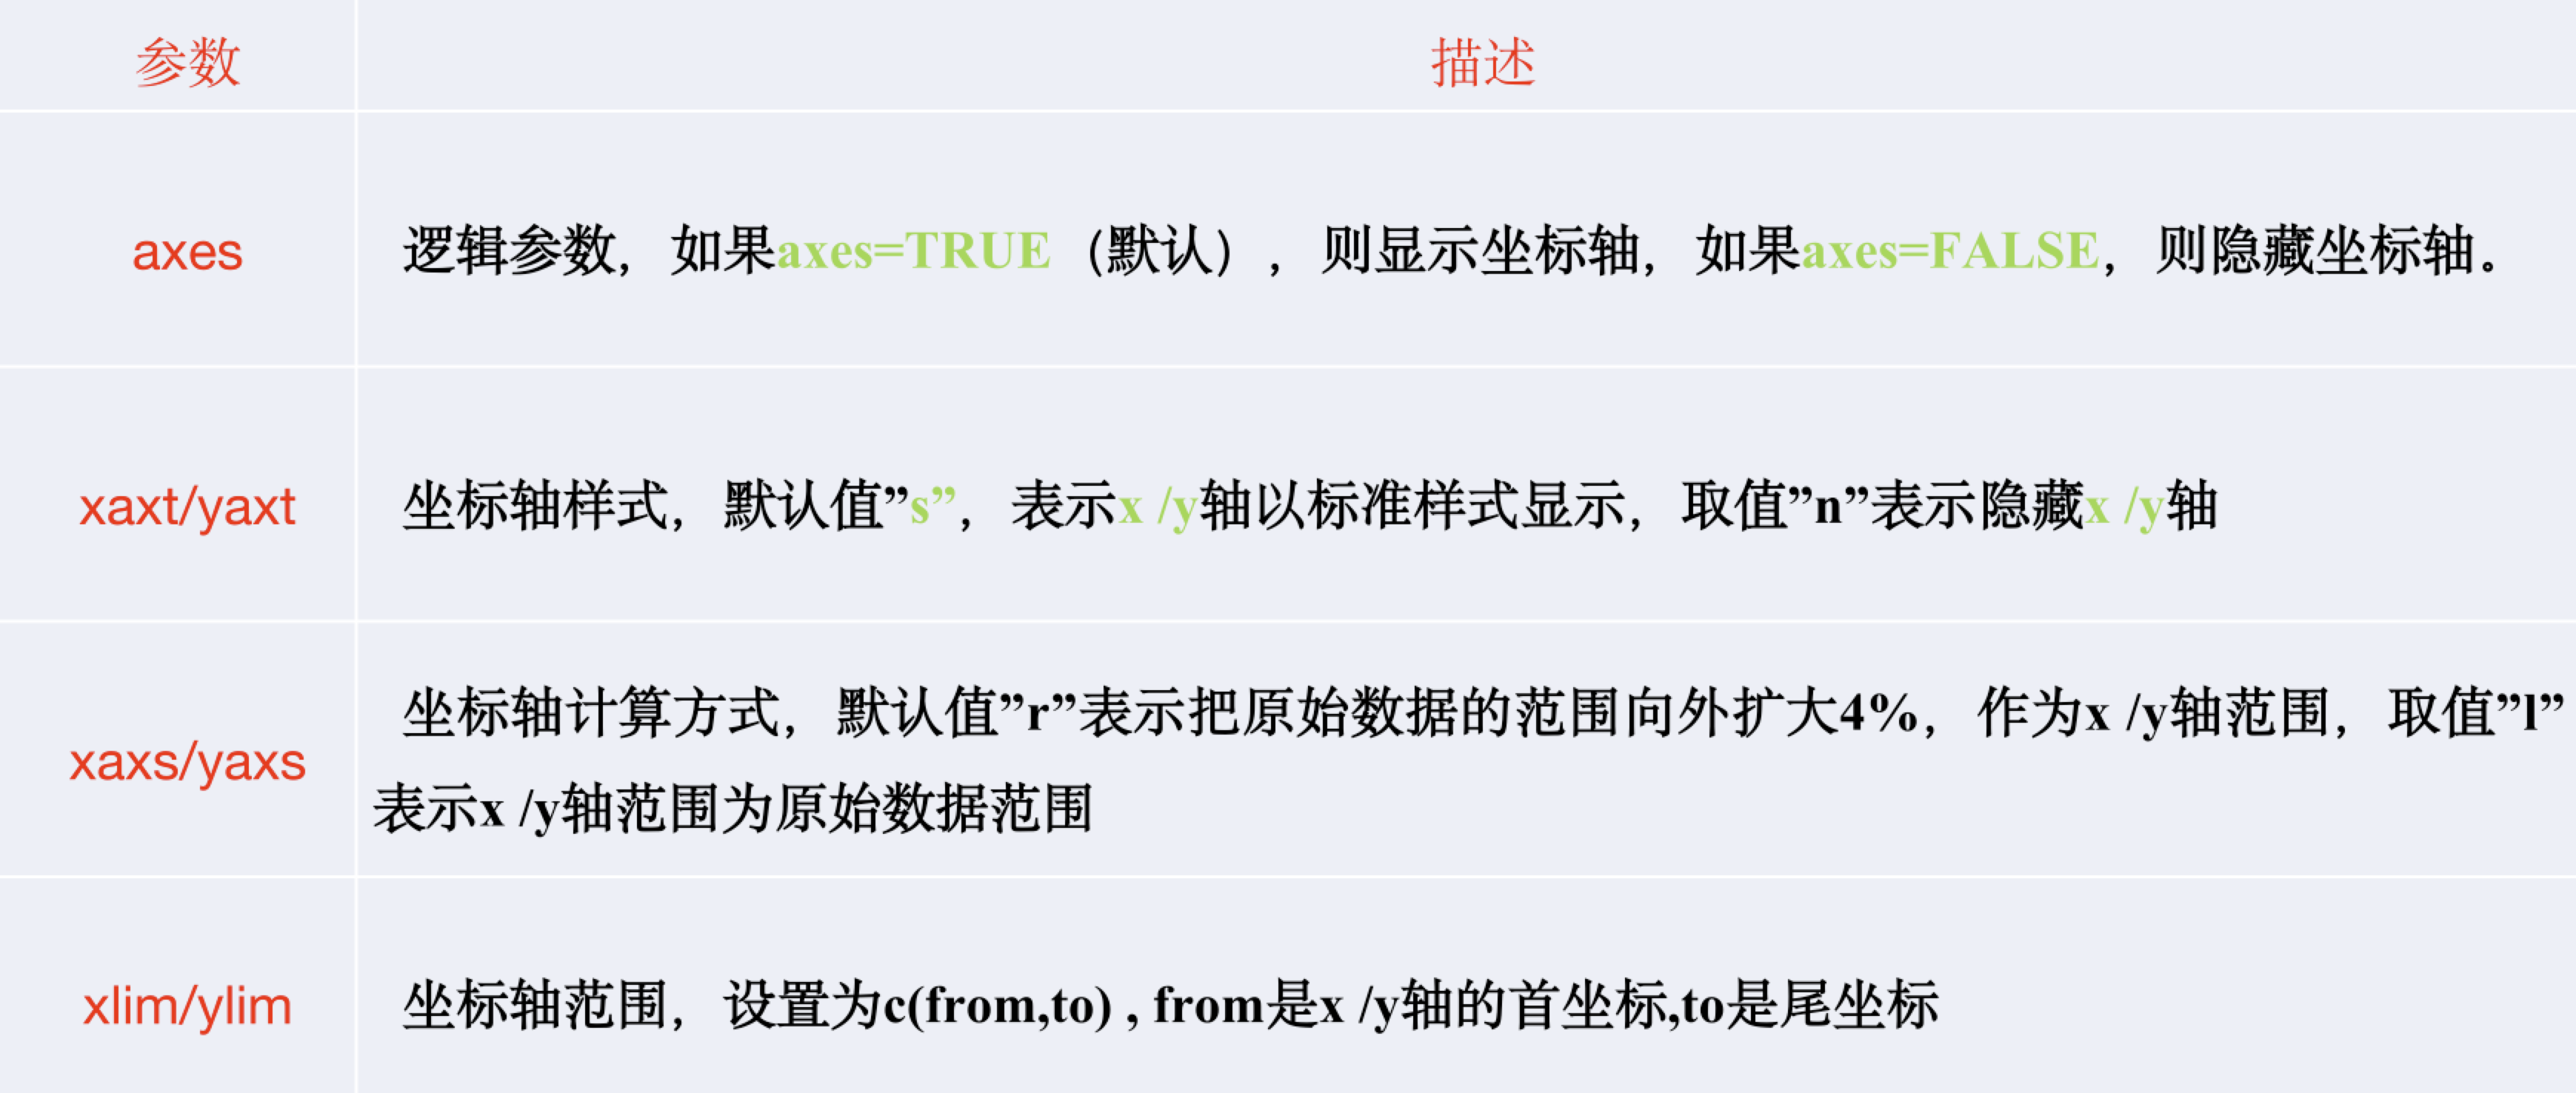
\includegraphics{figure/7.jpg}

\begin{Shaded}
\begin{Highlighting}[]
\FunctionTok{plot}\NormalTok{(}\FunctionTok{c}\NormalTok{(}\DecValTok{1}\SpecialCharTok{:}\DecValTok{12}\NormalTok{), }\AttributeTok{col=}\StringTok{"white"}\NormalTok{, }\AttributeTok{xaxt=}\StringTok{"n"}\NormalTok{, }\AttributeTok{yaxt=}\StringTok{"n"}\NormalTok{, }\AttributeTok{ann =} \ConstantTok{FALSE}\NormalTok{)}
\FunctionTok{axis}\NormalTok{(}\DecValTok{1}\NormalTok{, }\AttributeTok{at=}\DecValTok{1}\SpecialCharTok{:}\DecValTok{12}\NormalTok{, }\AttributeTok{col.axis=}\StringTok{"red"}\NormalTok{, }\AttributeTok{labels=}\NormalTok{month.abb)}
\FunctionTok{axis}\NormalTok{(}\DecValTok{2}\NormalTok{, }\AttributeTok{at=}\FunctionTok{seq}\NormalTok{(}\DecValTok{1}\NormalTok{,}\DecValTok{12}\NormalTok{,}\AttributeTok{length=}\DecValTok{10}\NormalTok{), }\AttributeTok{col.axis=}\StringTok{"red"}\NormalTok{, }\AttributeTok{labels=}\DecValTok{1}\SpecialCharTok{:}\DecValTok{10}\NormalTok{, }\AttributeTok{las=}\DecValTok{2}\NormalTok{)}
\FunctionTok{axis}\NormalTok{(}\DecValTok{3}\NormalTok{, }\AttributeTok{at=}\FunctionTok{seq}\NormalTok{(}\DecValTok{1}\NormalTok{,}\DecValTok{12}\NormalTok{,}\AttributeTok{length=}\DecValTok{7}\NormalTok{), }\AttributeTok{col.axis=}\StringTok{"blue"}\NormalTok{, }\AttributeTok{cex.axis=}\FloatTok{0.7}\NormalTok{, }
     \AttributeTok{tck=}\SpecialCharTok{{-}}\FloatTok{0.01}\NormalTok{, }\AttributeTok{labels =} \FunctionTok{c}\NormalTok{(}\StringTok{"Mon"}\NormalTok{, }\StringTok{"Tues"}\NormalTok{, }\StringTok{"Wed"}\NormalTok{, }\StringTok{"Thu"}\NormalTok{, }\StringTok{"Fri"}\NormalTok{, }\StringTok{"Sat"}\NormalTok{, }\StringTok{"Sun"}\NormalTok{)) }
\FunctionTok{axis}\NormalTok{(}\DecValTok{4}\NormalTok{, }\AttributeTok{at=}\FunctionTok{seq}\NormalTok{(}\DecValTok{1}\NormalTok{,}\DecValTok{12}\NormalTok{,}\AttributeTok{length=}\DecValTok{11}\NormalTok{), }\AttributeTok{col.axis=}\StringTok{"blue"}\NormalTok{, }\AttributeTok{cex.axis=}\FloatTok{0.7}\NormalTok{, }
     \AttributeTok{tck=}\SpecialCharTok{{-}}\FloatTok{0.01}\NormalTok{, }\AttributeTok{labels=}\FunctionTok{seq}\NormalTok{(}\DecValTok{0}\NormalTok{, }\DecValTok{1}\NormalTok{, }\FloatTok{0.1}\NormalTok{), }\AttributeTok{las=}\DecValTok{2}\NormalTok{)}
\end{Highlighting}
\end{Shaded}

\begin{center}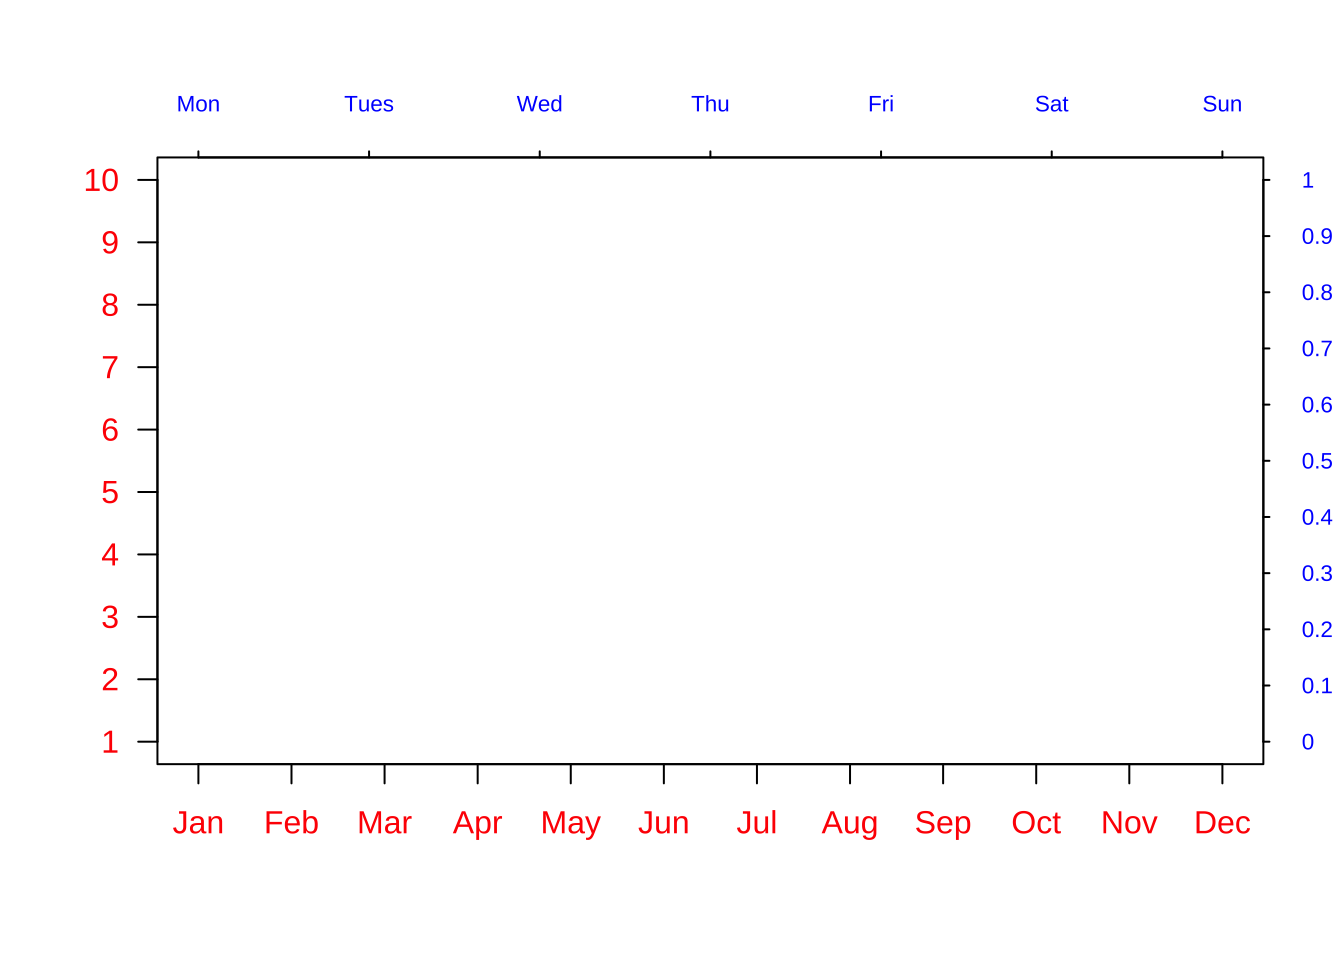
\includegraphics{1001-base-ploting_files/figure-latex/unnamed-chunk-32-1} \end{center}

\hypertarget{ux6dfbux52a0ux56feux4f8b}{%
\subsubsection{添加图例}\label{ux6dfbux52a0ux56feux4f8b}}

legend函数的绘制图例的位置效果

\begin{Shaded}
\begin{Highlighting}[]
\NormalTok{local}\OtherTok{=}\FunctionTok{c}\NormalTok{(}\StringTok{"bottomright"}\NormalTok{, }\StringTok{"bottom"}\NormalTok{, }\StringTok{"bottomleft"}\NormalTok{, }\StringTok{"left"}\NormalTok{, }\StringTok{"topleft"}\NormalTok{,}
        \StringTok{"top"}\NormalTok{, }\StringTok{"topright"}\NormalTok{, }\StringTok{"right"}\NormalTok{, }\StringTok{"center"}\NormalTok{)}
\FunctionTok{par}\NormalTok{(}\AttributeTok{mar =} \FunctionTok{c}\NormalTok{(}\DecValTok{4}\NormalTok{,}\DecValTok{2}\NormalTok{,}\DecValTok{4}\NormalTok{,}\DecValTok{2}\NormalTok{), }\AttributeTok{pty=}\StringTok{\textquotesingle{}m\textquotesingle{}}\NormalTok{)}
\FunctionTok{plot}\NormalTok{(}\FunctionTok{c}\NormalTok{(}\DecValTok{0}\SpecialCharTok{:}\DecValTok{10}\NormalTok{), }\AttributeTok{col =} \StringTok{"white"}\NormalTok{)}
\FunctionTok{legend}\NormalTok{(}\DecValTok{3}\NormalTok{, }\DecValTok{8}\NormalTok{, }\StringTok{"图例在(3,8)"}\NormalTok{)}
\ControlFlowTok{for}\NormalTok{(i }\ControlFlowTok{in} \DecValTok{1}\SpecialCharTok{:}\DecValTok{9}\NormalTok{)\{}
  \FunctionTok{legend}\NormalTok{(local[i], }\FunctionTok{paste}\NormalTok{(}\StringTok{"图例在"}\NormalTok{, local[i]))}
\NormalTok{\}}
\end{Highlighting}
\end{Shaded}

\begin{center}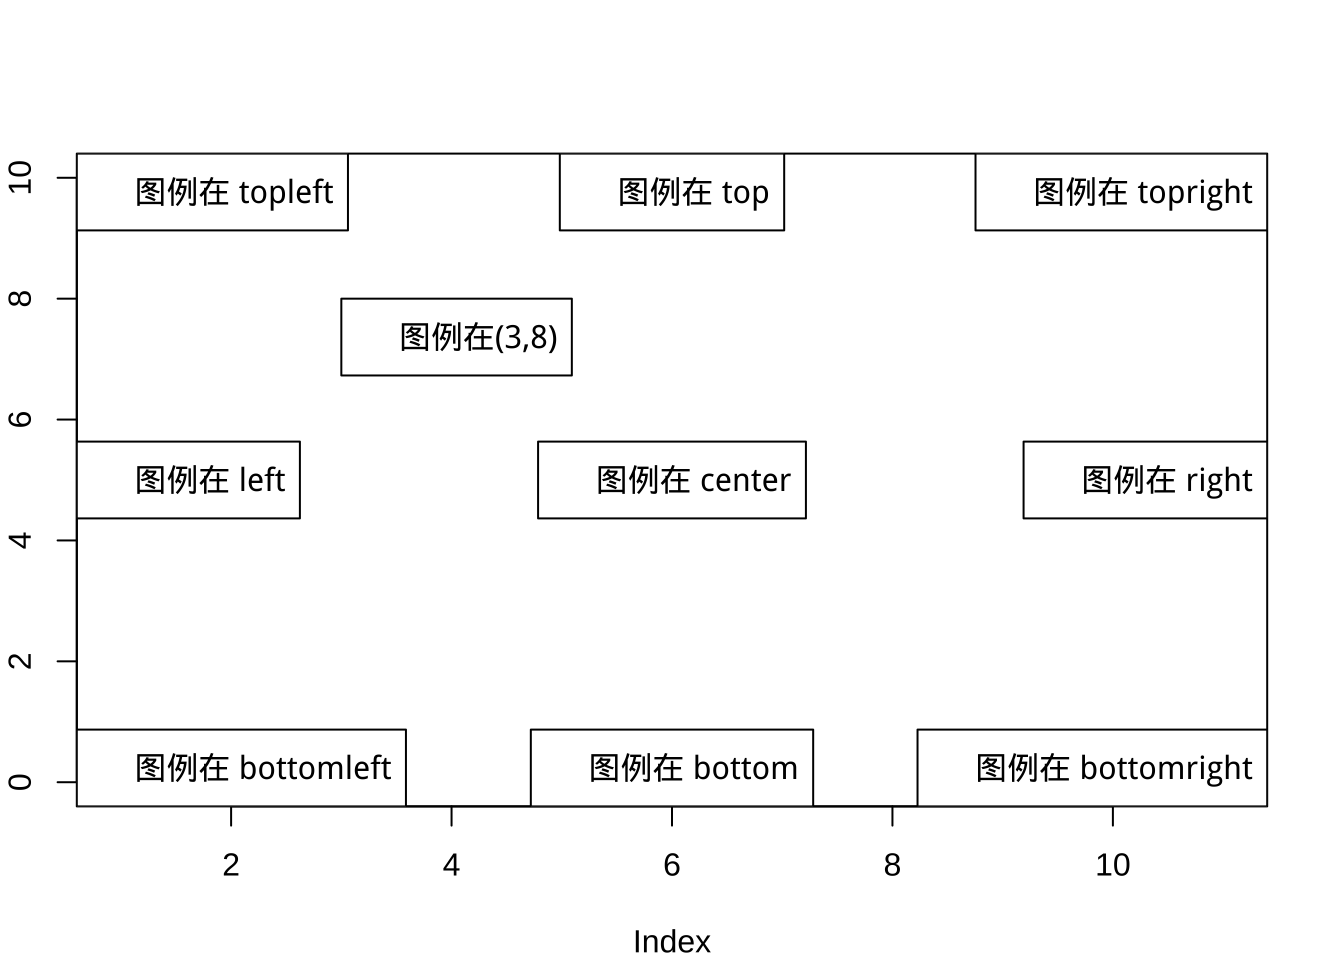
\includegraphics{1001-base-ploting_files/figure-latex/unnamed-chunk-33-1} \end{center}

\textbf{综合测试}:

\begin{Shaded}
\begin{Highlighting}[]
\FunctionTok{plot}\NormalTok{(iris}\SpecialCharTok{$}\NormalTok{Sepal.Length, iris}\SpecialCharTok{$}\NormalTok{Sepal.Width, }\AttributeTok{col =}\NormalTok{ iris}\SpecialCharTok{$}\NormalTok{Species, }
     \AttributeTok{main =} \FunctionTok{list}\NormalTok{(}\StringTok{\textquotesingle{}鸢尾花的花萼长与宽的散点图\textquotesingle{}}\NormalTok{, }\AttributeTok{cex =} \FloatTok{1.5}\NormalTok{), }
     \AttributeTok{xlab=}\StringTok{"花萼长度"}\NormalTok{, }\AttributeTok{ylab=}\StringTok{"花萼宽度"}\NormalTok{,}\AttributeTok{pch=}\DecValTok{19}\NormalTok{)}
\FunctionTok{grid}\NormalTok{(}\AttributeTok{nx=}\DecValTok{5}\NormalTok{, }\AttributeTok{ny=}\DecValTok{5}\NormalTok{, }\AttributeTok{lty=}\DecValTok{2}\NormalTok{, }\AttributeTok{col=}\StringTok{"grey"}\NormalTok{)  }\CommentTok{\# 添加网格线}
\FunctionTok{legend}\NormalTok{(}\DecValTok{7}\NormalTok{,}\FloatTok{4.5}\NormalTok{, }\FunctionTok{c}\NormalTok{(}\StringTok{\textquotesingle{}setosa\textquotesingle{}}\NormalTok{, }\StringTok{\textquotesingle{}versicolor\textquotesingle{}}\NormalTok{, }\StringTok{\textquotesingle{}virginica\textquotesingle{}}\NormalTok{),}
       \AttributeTok{pch=}\DecValTok{19}\NormalTok{, }\AttributeTok{col =} \DecValTok{1}\SpecialCharTok{:}\DecValTok{3}\NormalTok{)  }\CommentTok{\# 添加图例}
\FunctionTok{lines}\NormalTok{(}\FunctionTok{c}\NormalTok{(}\FloatTok{4.3}\NormalTok{, }\FloatTok{6.5}\NormalTok{), }\FunctionTok{c}\NormalTok{(}\DecValTok{2}\NormalTok{, }\FloatTok{4.5}\NormalTok{), }\AttributeTok{col =}\StringTok{\textquotesingle{}blue\textquotesingle{}}\NormalTok{)  }\CommentTok{\# 添加直线}
\FunctionTok{arrows}\NormalTok{(}\DecValTok{6}\NormalTok{, }\DecValTok{4}\NormalTok{ , }\FloatTok{6.5}\NormalTok{ ,}\DecValTok{4}\NormalTok{, }\AttributeTok{angle=}\DecValTok{10}\NormalTok{, }\AttributeTok{cex=}\FloatTok{0.5}\NormalTok{)  }\CommentTok{\# 添加箭头}
\FunctionTok{text}\NormalTok{(}\FloatTok{6.9}\NormalTok{, }\DecValTok{4}\NormalTok{, }\StringTok{"左上角全是setosa"}\NormalTok{, }\AttributeTok{cex=}\FloatTok{0.8}\NormalTok{)  }\CommentTok{\# 添加文字说明}
\end{Highlighting}
\end{Shaded}

\begin{center}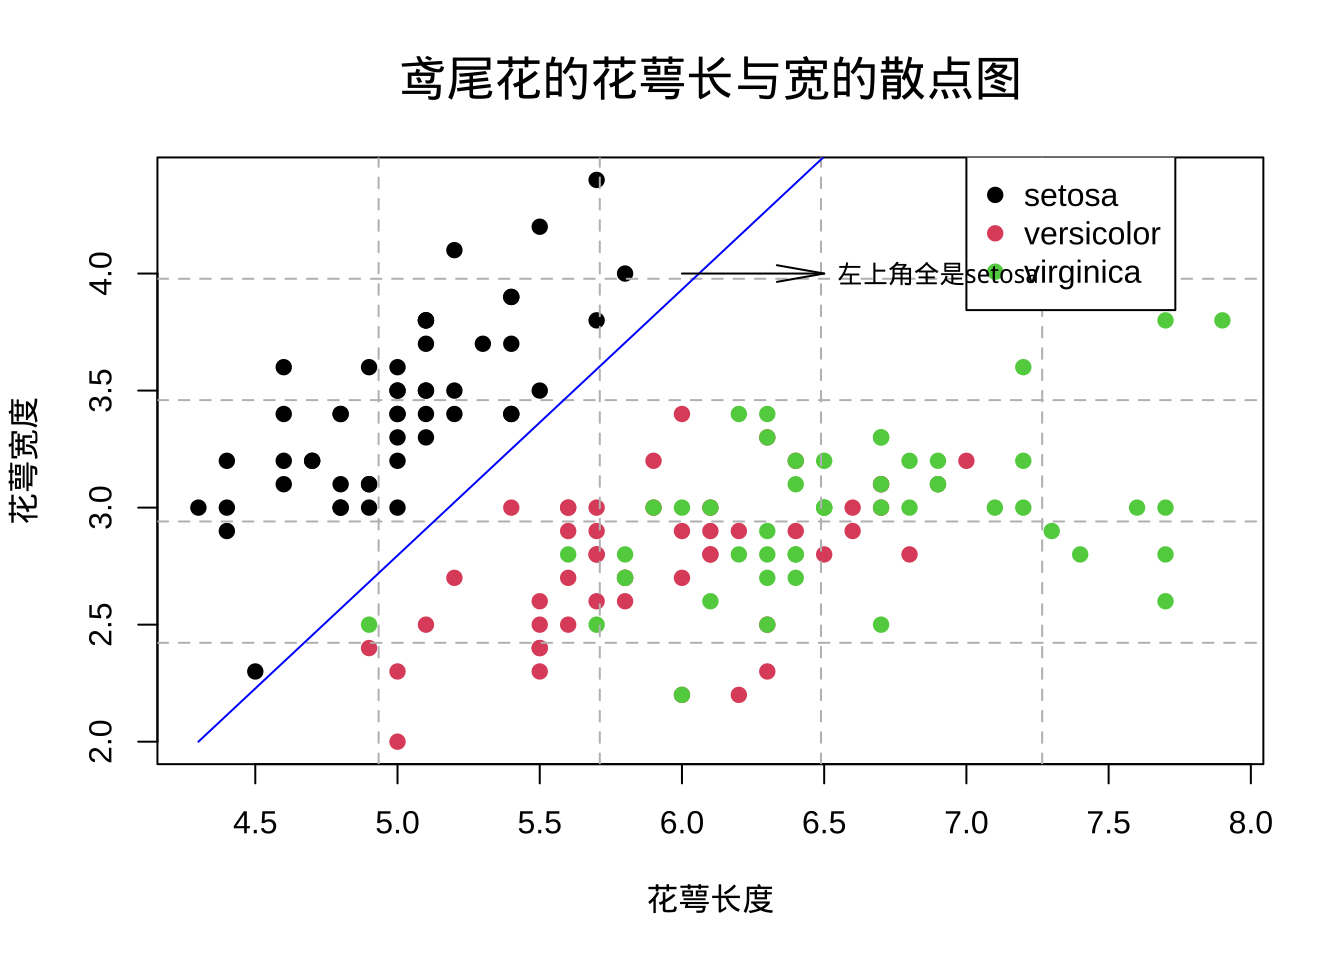
\includegraphics{1001-base-ploting_files/figure-latex/unnamed-chunk-34-1} \end{center}

\hypertarget{ux7ed8ux5236ux7ec4ux5408ux56feux5f62}{%
\section{绘制组合图形}\label{ux7ed8ux5236ux7ec4ux5408ux56feux5f62}}

\hypertarget{par}{%
\subsection{par()}\label{par}}

一页多图用mfrow参数或mfcol参数规定。

\begin{Shaded}
\begin{Highlighting}[]
\NormalTok{mfrow1}\OtherTok{=}\FunctionTok{par}\NormalTok{(}\AttributeTok{mfrow=}\FunctionTok{c}\NormalTok{(}\DecValTok{2}\NormalTok{,}\DecValTok{3}\NormalTok{)) }\CommentTok{\#mar=c(2,2,2,2)}
\ControlFlowTok{for}\NormalTok{(i }\ControlFlowTok{in} \DecValTok{1}\SpecialCharTok{:}\DecValTok{6}\NormalTok{)\{}
  \FunctionTok{plot}\NormalTok{(}\FunctionTok{c}\NormalTok{(}\DecValTok{1}\SpecialCharTok{:}\NormalTok{i),}\AttributeTok{main=}\FunctionTok{paste}\NormalTok{(}\StringTok{"I\textquotesingle{}m image:"}\NormalTok{,i))}
\NormalTok{\}}
\end{Highlighting}
\end{Shaded}

\begin{center}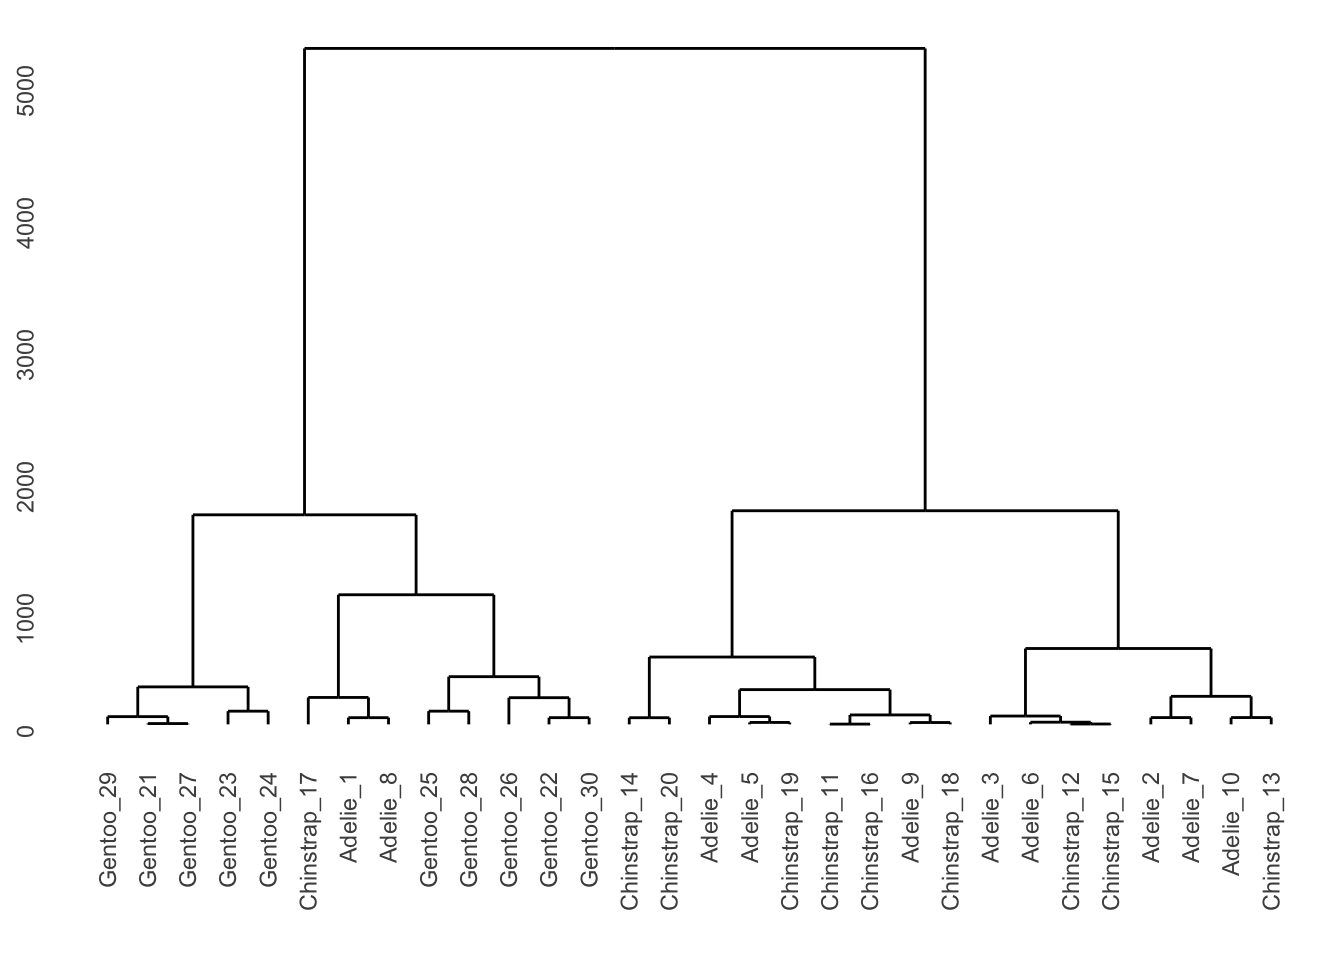
\includegraphics{1001-base-ploting_files/figure-latex/unnamed-chunk-35-1} \end{center}

\begin{Shaded}
\begin{Highlighting}[]
\FunctionTok{par}\NormalTok{(mfrow1)}

\NormalTok{op }\OtherTok{=} \FunctionTok{par}\NormalTok{(}\AttributeTok{mfrow=}\FunctionTok{c}\NormalTok{(}\DecValTok{2}\NormalTok{,}\DecValTok{2}\NormalTok{))}
\FunctionTok{plot}\NormalTok{(}\DecValTok{1}\SpecialCharTok{:}\DecValTok{10}\NormalTok{,}\AttributeTok{pch=}\DecValTok{12}\NormalTok{)}
\FunctionTok{hist}\NormalTok{(}\DecValTok{1}\SpecialCharTok{:}\DecValTok{10}\NormalTok{)}
\FunctionTok{boxplot}\NormalTok{(}\DecValTok{1}\SpecialCharTok{:}\DecValTok{10}\NormalTok{)}
\FunctionTok{pie}\NormalTok{(}\DecValTok{1}\SpecialCharTok{:}\DecValTok{10}\NormalTok{)}
\end{Highlighting}
\end{Shaded}

\begin{center}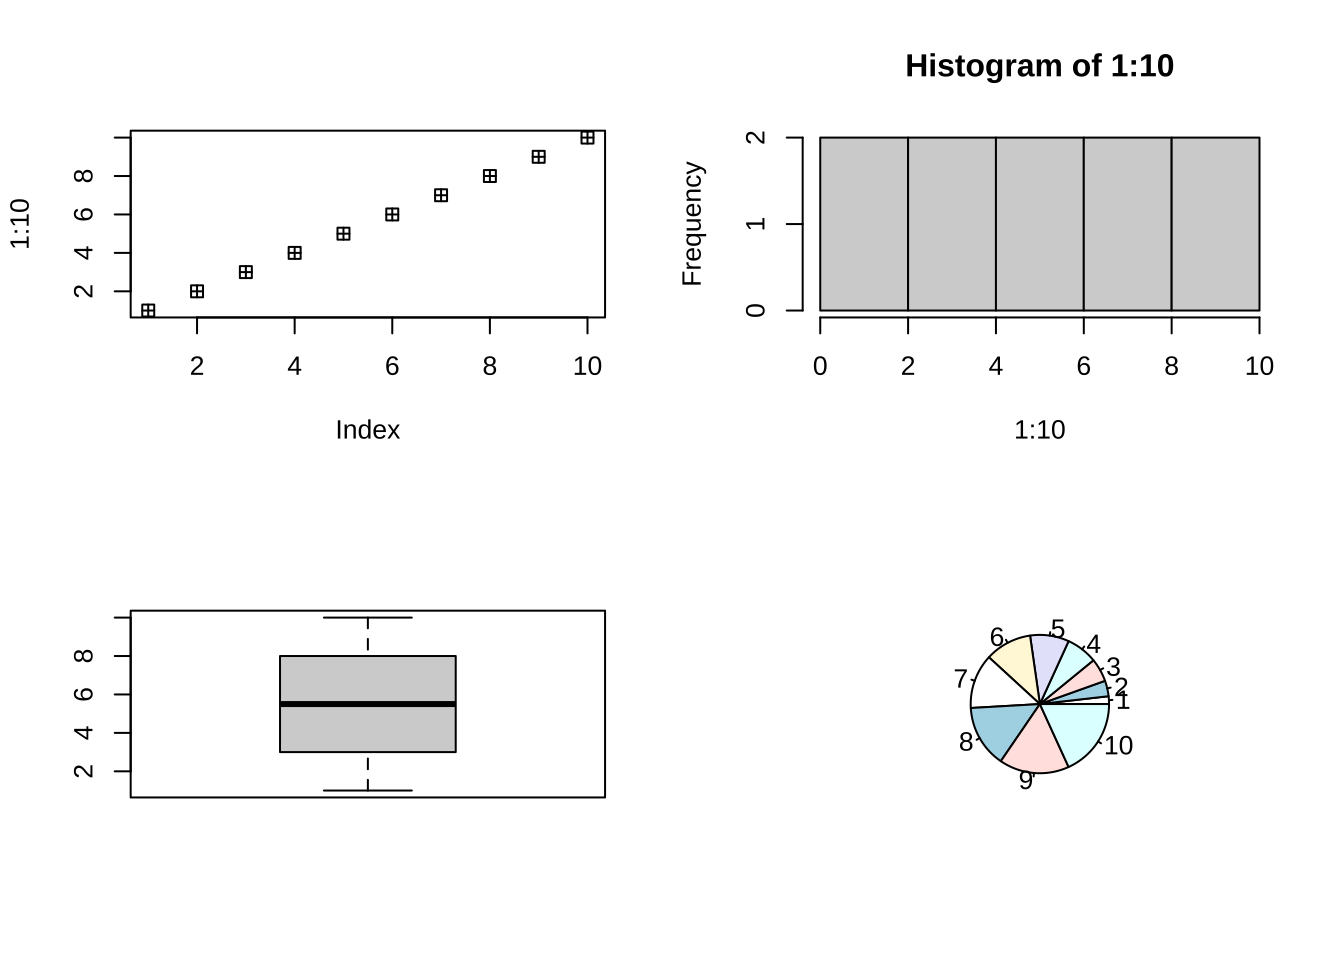
\includegraphics{1001-base-ploting_files/figure-latex/unnamed-chunk-35-2} \end{center}

\begin{Shaded}
\begin{Highlighting}[]
\FunctionTok{par}\NormalTok{(op)}
\end{Highlighting}
\end{Shaded}

\hypertarget{layout}{%
\subsection{layout}\label{layout}}

与par函数均分画布不同,layout函数可以不均等的分隔页面

\begin{Shaded}
\begin{Highlighting}[]
\NormalTok{mat}\OtherTok{\textless{}{-}}\FunctionTok{matrix}\NormalTok{(}\FunctionTok{c}\NormalTok{(}\DecValTok{1}\NormalTok{,}\DecValTok{1}\NormalTok{,}\DecValTok{1}\NormalTok{,}\DecValTok{2}\NormalTok{,}\DecValTok{3}\NormalTok{,}\DecValTok{3}\NormalTok{,}\DecValTok{4}\NormalTok{,}\DecValTok{4}\NormalTok{,}\DecValTok{5}\NormalTok{,}\DecValTok{5}\NormalTok{,}\DecValTok{5}\NormalTok{,}\DecValTok{6}\NormalTok{), }\AttributeTok{nrow =} \DecValTok{2}\NormalTok{, }\AttributeTok{byrow =} \ConstantTok{TRUE}\NormalTok{)}
\FunctionTok{layout}\NormalTok{(mat)}
\ControlFlowTok{for}\NormalTok{(i }\ControlFlowTok{in} \DecValTok{1}\SpecialCharTok{:}\DecValTok{6}\NormalTok{)\{}
  \FunctionTok{plot}\NormalTok{(}\FunctionTok{c}\NormalTok{(}\DecValTok{1}\SpecialCharTok{:}\NormalTok{i),}\AttributeTok{main=}\FunctionTok{paste}\NormalTok{(}\StringTok{"I\textquotesingle{}m image:"}\NormalTok{,i))}
\NormalTok{\}}
\end{Highlighting}
\end{Shaded}

\begin{center}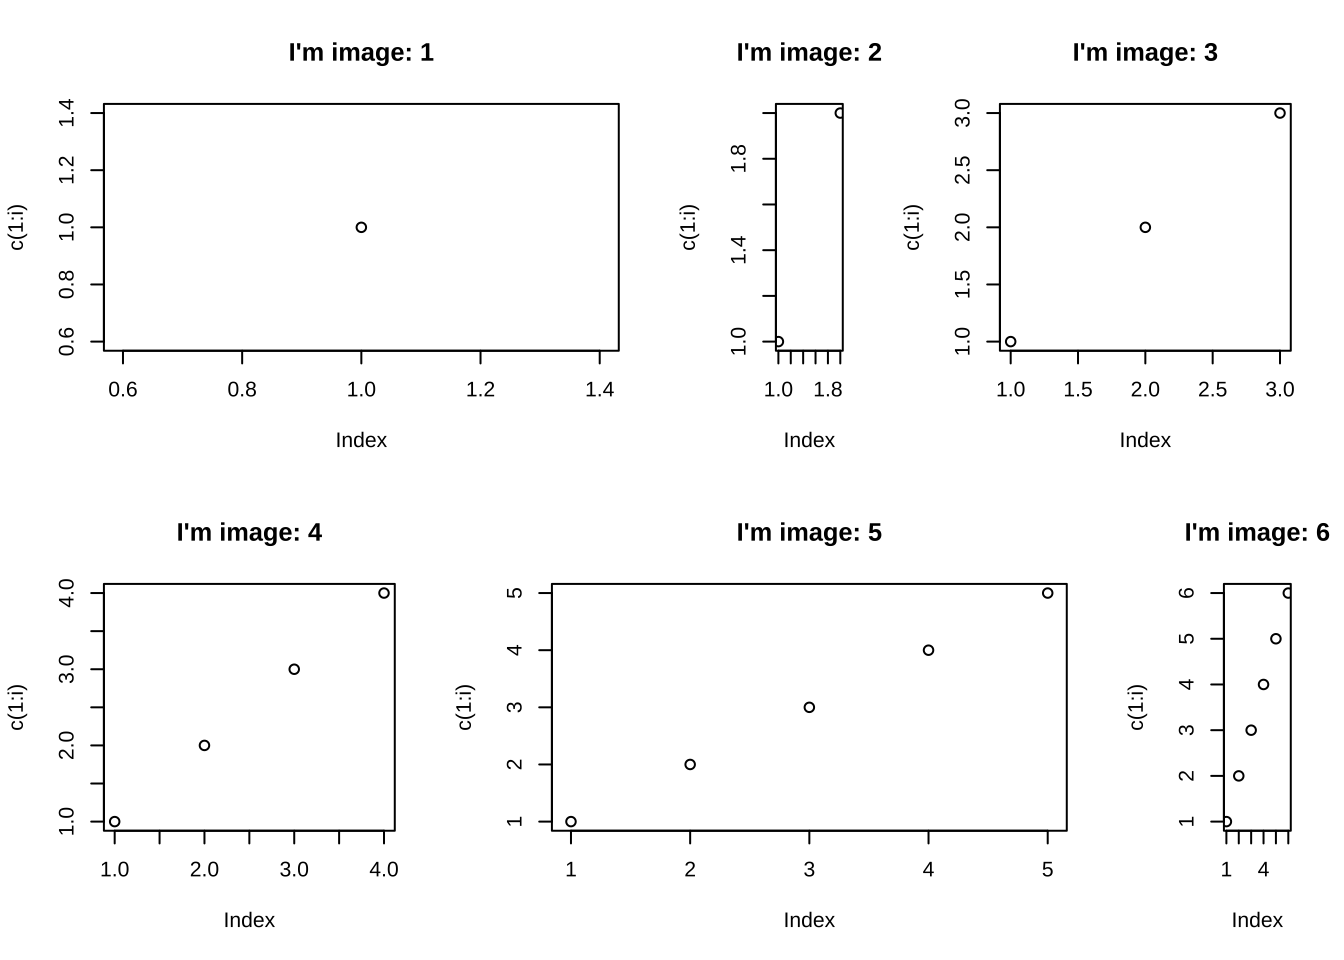
\includegraphics{1001-base-ploting_files/figure-latex/unnamed-chunk-36-1} \end{center}

\hypertarget{ux4fddux5b58ux56feux5f62}{%
\section{保存图形}\label{ux4fddux5b58ux56feux5f62}}

\hypertarget{ux4f7fux7528ux4ee3ux7801}{%
\subsection{使用代码}\label{ux4f7fux7528ux4ee3ux7801}}

对于其他格式输出类似pdf的输出。

\begin{Shaded}
\begin{Highlighting}[]
\FunctionTok{pdf}\NormalTok{(}\StringTok{"test/2.pdf"}\NormalTok{)  }\CommentTok{\# 保存到当前工作目录下}
\FunctionTok{plot}\NormalTok{(}\DecValTok{1}\SpecialCharTok{:}\DecValTok{10}\NormalTok{)}
\FunctionTok{dev.off}\NormalTok{()}
\end{Highlighting}
\end{Shaded}

\begin{verbatim}
## pdf 
##   2
\end{verbatim}

\hypertarget{ux5728-rstudio-ux7a97ux53e3ux70b9ux51fbux6309ux94aeux4fddux5b58}{%
\subsection{在 Rstudio 窗口点击按钮保存}\label{ux5728-rstudio-ux7a97ux53e3ux70b9ux51fbux6309ux94aeux4fddux5b58}}

\begin{figure}
\centering
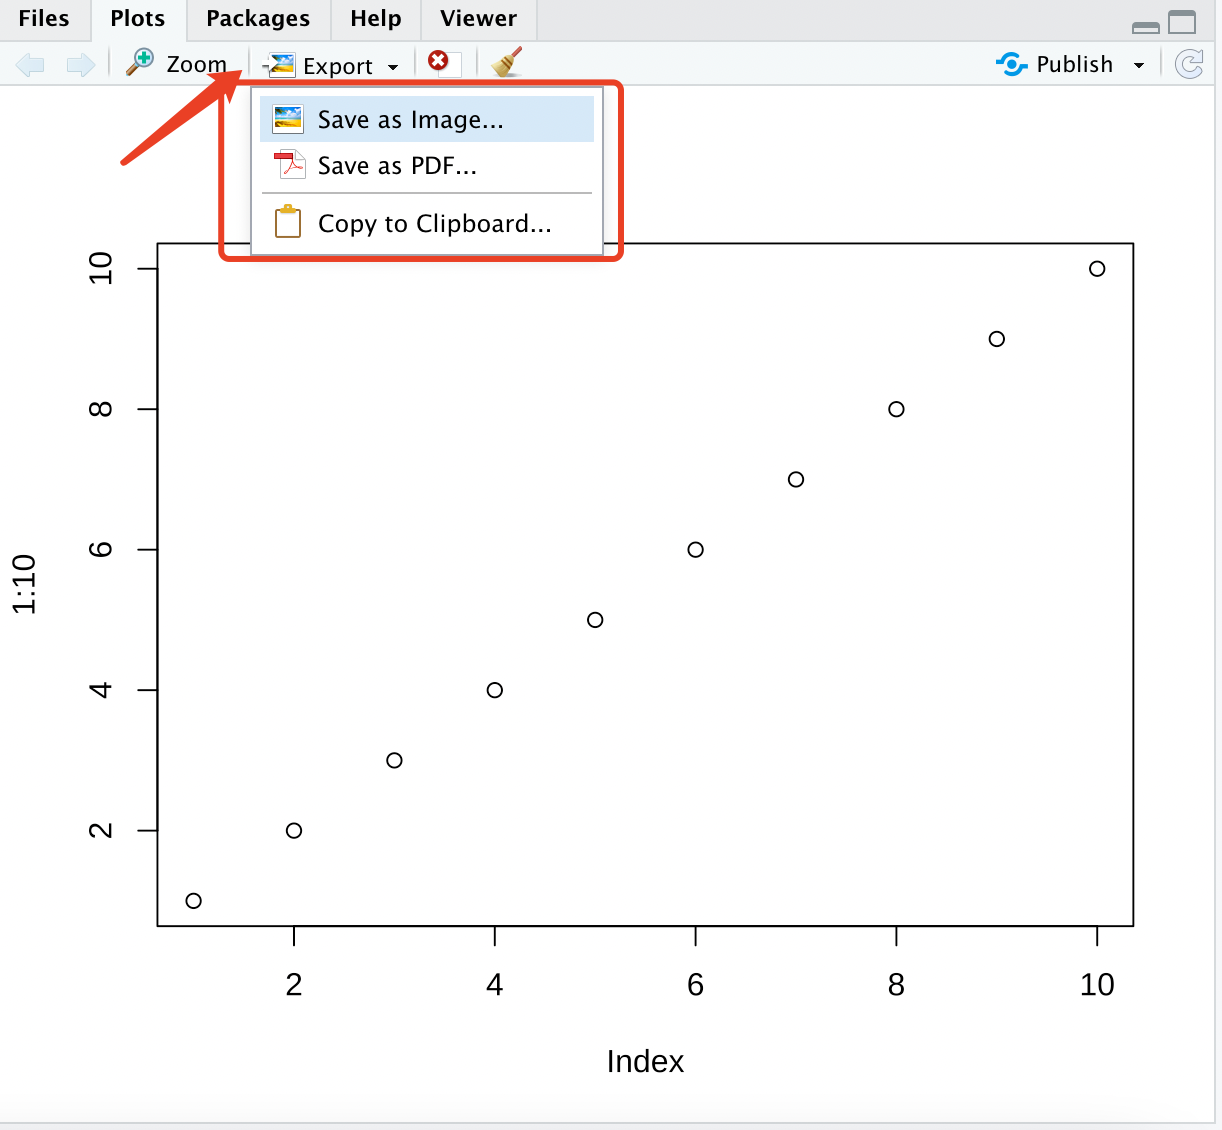
\includegraphics{figure/12.png}
\caption{Rstudio界面右下角}
\end{figure}

\begin{figure}
\centering
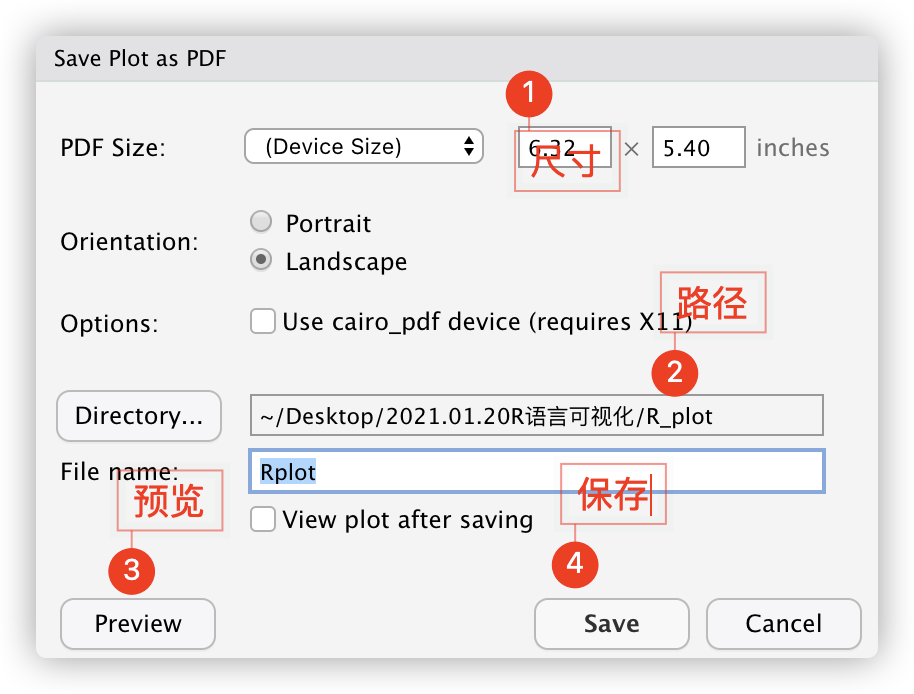
\includegraphics{figure/13.png}
\caption{自定义设置}
\end{figure}

\hypertarget{ggplot2-plot}{%
\chapter{使用 ggplot2 包绘图}\label{ggplot2-plot}}

\hypertarget{ux7b80ux4ecb-1}{%
\section{简介}\label{ux7b80ux4ecb-1}}

ggplot2 包是 Harley Wickham 在 2005
年创建的,是包含了一套全面而连贯的语法的绘图系统。

\begin{figure}
\centering

\includegraphics{figure/15.png}
\caption{Harley Wickham}
\end{figure}

弥补了R中创建图形缺乏一致性的缺点,且不会局限于一些已经定义好的统计图形,可以根据需要创造出任何有助于解决所遇到问题的图形。

\textbf{核心理念}:将绘图与数据分离,数据相关的绘图与数据无关的绘图分离,\textbf{按图层作图}。

\hypertarget{qplot}{%
\section{qplot}\label{qplot}}

\texttt{ggplot2}包的绘图语言与常用的绘图函数的使用方法不同,为了让读者快速使用\texttt{ggplot2}包,包的作者Harley
Wickham提供了\texttt{qplot}函数(quick
plot),让人在了解\texttt{ggplot2}的语言逻辑之前,就能迅速实现数据的可视化。

鸢尾花数据集\texttt{iris}

\begin{Shaded}
\begin{Highlighting}[]
\FunctionTok{head}\NormalTok{(iris,}\DecValTok{10}\NormalTok{)}
\end{Highlighting}
\end{Shaded}

\begin{verbatim}
##    Sepal.Length Sepal.Width Petal.Length Petal.Width Species
## 1           5.1         3.5          1.4         0.2  setosa
## 2           4.9         3.0          1.4         0.2  setosa
## 3           4.7         3.2          1.3         0.2  setosa
## 4           4.6         3.1          1.5         0.2  setosa
## 5           5.0         3.6          1.4         0.2  setosa
## 6           5.4         3.9          1.7         0.4  setosa
## 7           4.6         3.4          1.4         0.3  setosa
## 8           5.0         3.4          1.5         0.2  setosa
## 9           4.4         2.9          1.4         0.2  setosa
## 10          4.9         3.1          1.5         0.1  setosa
\end{verbatim}

\begin{Shaded}
\begin{Highlighting}[]
\FunctionTok{str}\NormalTok{(iris)}
\end{Highlighting}
\end{Shaded}

\begin{verbatim}
## 'data.frame':    150 obs. of  5 variables:
##  $ Sepal.Length: num  5.1 4.9 4.7 4.6 5 5.4 4.6 5 4.4 4.9 ...
##  $ Sepal.Width : num  3.5 3 3.2 3.1 3.6 3.9 3.4 3.4 2.9 3.1 ...
##  $ Petal.Length: num  1.4 1.4 1.3 1.5 1.4 1.7 1.4 1.5 1.4 1.5 ...
##  $ Petal.Width : num  0.2 0.2 0.2 0.2 0.2 0.4 0.3 0.2 0.2 0.1 ...
##  $ Species     : Factor w/ 3 levels "setosa","versicolor",..: 1 1 1 1 1 1 1 1 1 1 ...
\end{verbatim}

\begin{itemize}
\tightlist
\item
  \textbf{例子一:}
\end{itemize}

创建一个以物种种类为分组的花萼长度的箱线图,箱线图的颜色依据不同的物种种类而变化。

\begin{Shaded}
\begin{Highlighting}[]
\FunctionTok{library}\NormalTok{(ggplot2)}
\FunctionTok{qplot}\NormalTok{(Species, Sepal.Length, }\AttributeTok{data =}\NormalTok{ iris, }\AttributeTok{geom =} \StringTok{"boxplot"}\NormalTok{,}
      \AttributeTok{fill =}\NormalTok{ Species,}\AttributeTok{main =} \StringTok{"依据种类分组的花萼长度箱线图"}\NormalTok{)}
\end{Highlighting}
\end{Shaded}

\begin{center}\includegraphics{2001-ggplot-ploting_files/figure-latex/unnamed-chunk-3-1} \end{center}

\begin{Shaded}
\begin{Highlighting}[]
\FunctionTok{boxplot}\NormalTok{(Sepal.Length}\SpecialCharTok{\textasciitilde{}}\NormalTok{Species,}\AttributeTok{data =}\NormalTok{iris,}\AttributeTok{main =} \StringTok{"依据种类分组的花萼长度箱线图"}\NormalTok{)}
\end{Highlighting}
\end{Shaded}

\begin{center}\includegraphics{2001-ggplot-ploting_files/figure-latex/unnamed-chunk-3-2} \end{center}

\begin{itemize}
\tightlist
\item
  \textbf{例子二:}
\end{itemize}

利用\texttt{qplot}函数画出小提琴图,只需要将\texttt{geom}设置为\texttt{“violon”}即可,并添加扰动以减少数据重叠。

\begin{Shaded}
\begin{Highlighting}[]
\FunctionTok{qplot}\NormalTok{(Species, Sepal.Length, }\AttributeTok{data =}\NormalTok{ iris, }\AttributeTok{geom =} \FunctionTok{c}\NormalTok{(}\StringTok{"violin"}\NormalTok{, }\StringTok{"jitter"}\NormalTok{), }
      \AttributeTok{fill =}\NormalTok{ Species,}\AttributeTok{main =} \StringTok{"依据种类分组的花萼长度小提琴图"}\NormalTok{)}
\end{Highlighting}
\end{Shaded}

\begin{center}\includegraphics{2001-ggplot-ploting_files/figure-latex/unnamed-chunk-4-1} \end{center}

\begin{itemize}
\tightlist
\item
  \textbf{例子三:}
\end{itemize}

建一个以花萼长度和花萼宽度的散点图,并利用颜色和符号形状区分物种种类。

\begin{Shaded}
\begin{Highlighting}[]
\FunctionTok{qplot}\NormalTok{(Sepal.Length, Sepal.Width, }\AttributeTok{geom =} \StringTok{"point"}\NormalTok{,}\AttributeTok{data =}\NormalTok{ iris, }\AttributeTok{colour =}\NormalTok{ Species, }
      \AttributeTok{shape =}\NormalTok{ Species,}\AttributeTok{main =} \StringTok{"绘制花萼长度和花萼宽度的散点图"}\NormalTok{)}
\end{Highlighting}
\end{Shaded}

\begin{center}\includegraphics{2001-ggplot-ploting_files/figure-latex/unnamed-chunk-5-1} \end{center}

\begin{itemize}
\tightlist
\item
  \textbf{例子四:}
\end{itemize}

利用facets参数绘制分面板散点图,并增加光滑曲线。

\begin{Shaded}
\begin{Highlighting}[]
\FunctionTok{qplot}\NormalTok{(Sepal.Length, Sepal.Width, }\AttributeTok{data =}\NormalTok{ iris, }\AttributeTok{geom =} \FunctionTok{c}\NormalTok{(}\StringTok{"point"}\NormalTok{, }\StringTok{"smooth"}\NormalTok{),}
      \AttributeTok{facets =} \SpecialCharTok{\textasciitilde{}}\NormalTok{Species,}\AttributeTok{main =} \StringTok{"绘制分面板的散点图"}\NormalTok{)}
\end{Highlighting}
\end{Shaded}

\begin{center}\includegraphics{2001-ggplot-ploting_files/figure-latex/unnamed-chunk-6-1} \end{center}

\hypertarget{ggplot2ux5305ux56feux5f62ux8bedux6cd5}{%
\section{ggplot2包图形语法}\label{ggplot2ux5305ux56feux5f62ux8bedux6cd5}}

\textbf{推荐书籍}:

ggplot2: Elegant Graphics for Data Analysis \url{https://ggplot2-book.org/}

Fundamentals of Data Visualization \url{https://clauswilke.com/dataviz/}

\hypertarget{ux5bf9ux6bd4ux4e0dux540cux753bux56feux8bedux6cd5}{%
\subsection{对比不同画图语法}\label{ux5bf9ux6bd4ux4e0dux540cux753bux56feux8bedux6cd5}}

以绘制iris数据集中Sepal.Length与Sepal.Width的散点图为例,分别采用内置的plot函数与ggplot2包的ggplot函数绘制散点图,对比理解ggplot2包的语言逻辑。

代码(三种类型):

\begin{Shaded}
\begin{Highlighting}[]
\CommentTok{\# 基础包}
\FunctionTok{plot}\NormalTok{(iris}\SpecialCharTok{$}\NormalTok{Sepal.Length, iris}\SpecialCharTok{$}\NormalTok{Sepal.Width)}
\end{Highlighting}
\end{Shaded}

\begin{center}\includegraphics{2001-ggplot-ploting_files/figure-latex/unnamed-chunk-8-1} \end{center}

\begin{Shaded}
\begin{Highlighting}[]
\CommentTok{\# qplot()}
\FunctionTok{qplot}\NormalTok{(}\AttributeTok{x =}\NormalTok{ Sepal.Length, }\AttributeTok{y =}\NormalTok{ Sepal.Width,}\AttributeTok{data =}\NormalTok{ iris,}\AttributeTok{geom =} \StringTok{"point"}\NormalTok{)}
\end{Highlighting}
\end{Shaded}

\begin{center}\includegraphics{2001-ggplot-ploting_files/figure-latex/unnamed-chunk-8-2} \end{center}

\begin{Shaded}
\begin{Highlighting}[]
\CommentTok{\# ggplot()}
\FunctionTok{ggplot}\NormalTok{(}\AttributeTok{data=}\NormalTok{ iris, }\FunctionTok{aes}\NormalTok{(}\AttributeTok{x =}\NormalTok{ Sepal.Length, }\AttributeTok{y =}\NormalTok{ Sepal.Width)) }\SpecialCharTok{+}  \CommentTok{\#绘制底层画布}
\FunctionTok{geom\_point}\NormalTok{()  }\CommentTok{\#在画布上添加点}
\end{Highlighting}
\end{Shaded}

\begin{center}\includegraphics{2001-ggplot-ploting_files/figure-latex/unnamed-chunk-8-3} \end{center}

\hypertarget{ux601dux60f3ux4ecbux7ecd}{%
\subsection{思想介绍}\label{ux601dux60f3ux4ecbux7ecd}}

\textbf{注:}该部分主要参考\href{https://bookdown.org/wangminjie/R4DS/intro-R.html\#\%E5\%AE\%89\%E8\%A3\%85-rstudio}{数据科学中的R语言------王敏杰}。

ggplot的绘图有以下几个特点。

\begin{enumerate}
\def\labelenumi{\arabic{enumi}.}
\item
  有明确的起始(以ggplot函数开始)与终止(一句语句一幅图)。
\item
  ggplot2语句可以理解为一句语句绘制一幅图,然后进行图层叠加,而叠加是通过''+``号把绘图语句拼接实现的。
\end{enumerate}

ggplot函数包括9个部件:

\begin{itemize}
\tightlist
\item
  数据 (data) ( 数据框)
\item
  映射 (mapping)
\item
  几何对象 (geom\_point() , geom\_boxplot())
\item
  统计变换 (stats)
\item
  标度 (scale)
\item
  坐标系 (coord)
\item
  分面 (facet)
\item
  主题 (theme)
\item
  存储和输出 (output)
\end{itemize}

其中前三个是必需的。

Hadley
Wickham将这套可视化语法诠释为:一张统计图形就是从\textbf{数据}到\textbf{几何对象}(geometric
object,缩写geom)的\textbf{图形属性}(aesthetic
attribute,缩写aes)的一个映射。

\includegraphics{figure/10.png}

此外,图形中还可能包含数据的\textbf{统计变换}(statistical
transformation,缩写stats),最后绘制在某个特定的\textbf{坐标系}(coordinate
system,缩写coord)中,而\textbf{分面}(facet)则可以用来生成数据不同子集的图形。

\begin{figure}
\centering
\includegraphics{figure/11.png}
\caption{语法模板}
\end{figure}

\begin{figure}
\centering
\includegraphics{figure/22.png}
\caption{把这看懂其实差不多了}
\end{figure}

\textbf{例子(带你入门)}

\begin{Shaded}
\begin{Highlighting}[]
\FunctionTok{ggplot}\NormalTok{(}\AttributeTok{data =}\NormalTok{ iris, }\AttributeTok{mapping =} \FunctionTok{aes}\NormalTok{(Petal.Length,Petal.Width)) }\SpecialCharTok{+}
  \FunctionTok{geom\_point}\NormalTok{(}\AttributeTok{size =} \DecValTok{2}\NormalTok{,}\AttributeTok{alpha =} \FloatTok{0.5}\NormalTok{,}\AttributeTok{col =}\StringTok{"red"}\NormalTok{) }\SpecialCharTok{+}
  \FunctionTok{geom\_smooth}\NormalTok{(}\AttributeTok{method =} \StringTok{"lm"}\NormalTok{,}\AttributeTok{se =}\NormalTok{ F)}
\end{Highlighting}
\end{Shaded}

\begin{center}\includegraphics{2001-ggplot-ploting_files/figure-latex/unnamed-chunk-9-1} \end{center}

\hypertarget{ux5168ux5c40ux53d8ux91cf-vs.-ux5c40ux90e8ux53d8ux91cf}{%
\subsection{全局变量 vs.~局部变量}\label{ux5168ux5c40ux53d8ux91cf-vs.-ux5c40ux90e8ux53d8ux91cf}}

\begin{Shaded}
\begin{Highlighting}[]
\FunctionTok{ggplot}\NormalTok{(}\AttributeTok{data =}\NormalTok{ iris, }\AttributeTok{mapping =} \FunctionTok{aes}\NormalTok{(}\AttributeTok{x =}\NormalTok{ Petal.Length,}\AttributeTok{y =}\NormalTok{ Petal.Width, }\AttributeTok{col =}\NormalTok{ Species)) }\SpecialCharTok{+}
  \FunctionTok{geom\_point}\NormalTok{() }
\end{Highlighting}
\end{Shaded}

\begin{center}\includegraphics{2001-ggplot-ploting_files/figure-latex/unnamed-chunk-10-1} \end{center}

\begin{Shaded}
\begin{Highlighting}[]
\FunctionTok{ggplot}\NormalTok{(}\AttributeTok{data =}\NormalTok{ iris) }\SpecialCharTok{+}
  \FunctionTok{geom\_point}\NormalTok{(}\AttributeTok{mapping =} \FunctionTok{aes}\NormalTok{(}\AttributeTok{x =}\NormalTok{ Petal.Length,}\AttributeTok{y =}\NormalTok{ Petal.Width, }\AttributeTok{col =}\NormalTok{ Species))}
\end{Highlighting}
\end{Shaded}

\begin{center}\includegraphics{2001-ggplot-ploting_files/figure-latex/unnamed-chunk-10-2} \end{center}

大家可以看到,以上两段代码出来的图是一样。但背后的含义却不同。

\textbf{例子(观察两者之间的区别)}

\begin{Shaded}
\begin{Highlighting}[]
\CommentTok{\#版本一}
\FunctionTok{ggplot}\NormalTok{(}\AttributeTok{data =}\NormalTok{ iris, }\AttributeTok{mapping =} \FunctionTok{aes}\NormalTok{(}\AttributeTok{x =}\NormalTok{ Petal.Length,}\AttributeTok{y =}\NormalTok{ Petal.Width, }\AttributeTok{col =}\NormalTok{ Species)) }\SpecialCharTok{+}
  \FunctionTok{geom\_point}\NormalTok{() }\SpecialCharTok{+} 
  \FunctionTok{geom\_smooth}\NormalTok{() }
\end{Highlighting}
\end{Shaded}

\begin{center}\includegraphics{2001-ggplot-ploting_files/figure-latex/unnamed-chunk-11-1} \end{center}

\begin{Shaded}
\begin{Highlighting}[]
\CommentTok{\# 版本二}
\FunctionTok{ggplot}\NormalTok{(}\AttributeTok{data =}\NormalTok{ iris, }\AttributeTok{mapping =} \FunctionTok{aes}\NormalTok{(}\AttributeTok{x =}\NormalTok{ Petal.Length,}\AttributeTok{y =}\NormalTok{ Petal.Width)) }\SpecialCharTok{+}
  \FunctionTok{geom\_point}\NormalTok{(}\AttributeTok{mapping =} \FunctionTok{aes}\NormalTok{(}\AttributeTok{col =}\NormalTok{ Species)) }\SpecialCharTok{+} 
  \FunctionTok{geom\_smooth}\NormalTok{()}
\end{Highlighting}
\end{Shaded}

\begin{center}\includegraphics{2001-ggplot-ploting_files/figure-latex/unnamed-chunk-11-2} \end{center}

\hypertarget{ux51e0ux4f55ux5bf9ux8c61}{%
\section{几何对象}\label{ux51e0ux4f55ux5bf9ux8c61}}

\texttt{geom\_xxx()}提供了各种基本图形。 列表如下:

\begin{itemize}
\item
  基础图形:

  \begin{itemize}
  \tightlist
  \item
    \texttt{geom\_blank()}不画图,可以按映射的变量设定坐标范围;
  \item
    \texttt{geom\_point()}每个观测为一个散点;
  \item
    \texttt{geom\_hline()}, \texttt{geom\_vline()}, \texttt{geom\_abline()}画线;
  \item
    \texttt{geom\_path()}每个观测提供坐标,在相邻观测之间连线;
  \item
    \texttt{geom\_ribbon()}需要x和ymin,
    ymax维,在从小到大排序后的相邻观测之间连接阴影区域;
  \item
    \texttt{geom\_segment()}需要x, y和xend, yend,为每个观测画一条线段;
  \item
    \texttt{geom\_rect()}需要xmin, xmax, ymin,
    ymax,为每个观测画一个长方形,可有填充色;
  \item
    \texttt{geom\_polygon()}需要x,
    y,将相邻观测连续并连接成一个闭合的多边形,中间填充颜色;
  \item
    \texttt{geom\_text()}需要x, y和lable,每个观测画一条文字标签。
  \end{itemize}
\item
  单变量图层:

  \begin{itemize}
  \tightlist
  \item
    \texttt{geom\_bar()}, \texttt{geom\_col()}作条形图;
  \item
    \texttt{geom\_histogram()}对连续变量x作直方图;
  \item
    \texttt{geom\_density()}对连续变量x作一元密度估计曲线;
  \item
    \texttt{geom\_dotplot()}用原点作直方图;
  \item
    \texttt{geom\_freqpoly()}用折线作直方图。
  \end{itemize}
\item
  两变量图形:

  \begin{itemize}
  \item
    两个连续变量x, y:

    \begin{itemize}
    \tightlist
    \item
      \texttt{geom\_point()}散点图;
    \item
      \texttt{geom\_quantile()}拟合分位数回归曲线;
    \item
      \texttt{geom\_rug()}在坐标轴处画数值对应的短须线;
    \item
      \texttt{geom\_smooth()}画各种拟合曲线;
    \item
      \texttt{geom\_text()}在指定的x, y位置画label给出的文字标签;
    \end{itemize}
  \item
    显示二元分布:

    \begin{itemize}
    \tightlist
    \item
      \texttt{geom\_bin2d()}作长方形分块的二维直方图;
    \item
      \texttt{geom\_density2d()}作二元密度估计等值线图;
    \item
      \texttt{geom\_hex()}作正六边形分块的二维直方图。
    \end{itemize}
  \item
    两个变量中有分类变量时:

    \begin{itemize}
    \tightlist
    \item
      \texttt{geom\_count()}:重叠点越多画点越大;
    \item
      \texttt{geom\_jitter()}:
      随机扰动散点位置避免重叠,数值变量有重叠时也可以用;
    \end{itemize}
  \item
    一个连续变量和一个分类变量:

    \begin{itemize}
    \tightlist
    \item
      \texttt{geom\_col()}作条形图,对分类变量的每个值画一个条形,长度与连续变量值成比例;
    \item
      \texttt{geom\_boxplot()}对每个类做一个盒形图;
    \item
      \texttt{geom\_violin()}对每个类做一个小提琴图。
    \end{itemize}
  \item
    一个时间变量和一个连续变量:

    \begin{itemize}
    \tightlist
    \item
      \texttt{geom\_area()}作阴影曲线图,曲线下方填充阴影色;
    \item
      \texttt{geom\_line()}作折线图,在相邻两个时间之间连接线段;
    \item
      \texttt{geom\_step()}作阶梯函数图,在相邻两个时间之间连接阶梯函数线。
    \end{itemize}
  \item
    不确定性:

    \begin{itemize}
    \tightlist
    \item
      \texttt{geom\_crossbar()}对每个观测输入的x, y, ymin,
      ymax画中间有线的纵向条形;
    \item
      \texttt{geom\_errbar()}对每个观测输入的x, ymin, ymax画纵向误差条;
    \item
      \texttt{geom\_linerange()}对每个观测输入的x, ymin, ymax画一条竖线;
    \item
      \texttt{geom\_pointrnage()}对每个观测输入的x, y, ymin,
      ymax画一条中间有点的竖线。
    \end{itemize}
  \end{itemize}
\item
  地图:

  \begin{itemize}
  \tightlist
  \item
    \texttt{geom\_map()}: 用区域边界坐标数据画边界线地图。
  \end{itemize}
\item
  三个变量:

  \begin{itemize}
  \item
    \texttt{geom\_contour()}: 用输入的x, y, z数据画等值线图。
  \item
    \texttt{geom\_tile()}用输入的x, y位置, width,
    height大小和指定的fill维画长方形色块填充图。
  \item
    \texttt{geom\_raster()}是\texttt{geom\_tile()}的长方形大小相同时的快速版本。
  \end{itemize}
\end{itemize}

\hypertarget{ux53c2ux8003ux4e66ux7c4d}{%
\subsection{参考书籍}\label{ux53c2ux8003ux4e66ux7c4d}}

由于这部分内容非常的多,短短两小时不可能讲完,这里给了一些参考资料,各个都是满满的干货。

\begin{itemize}
\item
  \href{https://bookdown.org/wangminjie/R4DS/ggplot2-geom.html\#\%E5\%9F\%BA\%E6\%9C\%AC\%E7\%BB\%98\%E5\%9B\%BE}{数据科学中的R-第14章ggplot之集合对象}
\item
  \href{https://www.math.pku.edu.cn/teachers/lidf/docs/Rbook/html/_Rbook/ggplotvis.html}{R语言教程第30节-ggplot各种图形}
\item
  \href{http://r-statistics.co/Top50-Ggplot2-Visualizations-MasterList-R-Code.html}{Top 50 ggplot2
  Visualizations}
\item
  \href{http://r4ds.had.co.nz/data-visualisation.html}{Chapter 3: Data
  Visualisation} of \emph{R
  for Data Science}
\item
  \href{http://r4ds.had.co.nz/graphics-for-communication.html}{Chapter 28: Graphics for
  communication}
  of \emph{R for Data Science}
\item
  \href{https://r-graphics.org/}{Graphs} in \emph{R Graphics Cookbook}
\end{itemize}

\hypertarget{ux7edfux8ba1ux53d8ux6362}{%
\section{统计变换}\label{ux7edfux8ba1ux53d8ux6362}}

\textbf{概念}:对数据所应用的统计类型/方法。

ggplot2为每一种几何类型指定了一种默认的统计类型,如果仅指定geom或stat中的一个,另外一个会自动获取。其中,stat\_identity则表示不做任何的统计变换。

\textbf{示例}:只需指定geom或stat中的一个,具体细小细节可以参考这
\url{https://bookdown.org/wangminjie/R4DS/ggplot2-stat-layer.html}

\begin{Shaded}
\begin{Highlighting}[]
\FunctionTok{ggplot}\NormalTok{(iris) }\SpecialCharTok{+} 
  \FunctionTok{geom\_bar}\NormalTok{(}\FunctionTok{aes}\NormalTok{(}\AttributeTok{x=}\NormalTok{Sepal.Length), }\AttributeTok{stat=}\StringTok{"bin"}\NormalTok{, }\AttributeTok{binwidth =} \FloatTok{0.5}\NormalTok{)}
\end{Highlighting}
\end{Shaded}

\begin{center}\includegraphics{2001-ggplot-ploting_files/figure-latex/unnamed-chunk-12-1} \end{center}

\begin{Shaded}
\begin{Highlighting}[]
\FunctionTok{ggplot}\NormalTok{(iris) }\SpecialCharTok{+} 
  \FunctionTok{stat\_bin}\NormalTok{(}\FunctionTok{aes}\NormalTok{(}\AttributeTok{x=}\NormalTok{Sepal.Length), }\AttributeTok{geom=}\StringTok{"bar"}\NormalTok{, }\AttributeTok{binwidth =} \FloatTok{0.5}\NormalTok{)}
\end{Highlighting}
\end{Shaded}

\begin{center}\includegraphics{2001-ggplot-ploting_files/figure-latex/unnamed-chunk-12-2} \end{center}

\hypertarget{ux523bux5ea6scale}{%
\section{刻度scale}\label{ux523bux5ea6scale}}

这一节我们一起学习ggplot2中的scales语法,推荐大家阅读Hadley
Wickham最新版的\href{https://ggplot2-book.org/}{《ggplot2: Elegant Graphics for Data
Analysis》},但如果需要详细了解\textbf{标度}参数体系,还是要看\href{https://cran.r-project.org/web/packages/ggplot2/index.html}{ggplot2官方文档}

在\texttt{ggplot()}的mapping参数中指定x维、y维、color维等,实际上每一维度都有一个\textbf{对应的默认刻度}(scale),即,将\textbf{数据值映射到图形中的映射方法}。

如果需要修改刻度对应的变换或者标度方法,可以调用相应的scale\_xxx()函数。

\textbf{画图都没用到scale啊!}

能画个很漂亮的图,那是因为ggplot2默认缺省条件下,已经很美观了。(据说Hadley
Wickham很后悔使用了这么漂亮的缺省值,因为很漂亮了大家都不认真学画图了。马云好像也说后悔创立了阿里巴巴?)

\begin{Shaded}
\begin{Highlighting}[]
\CommentTok{\#解释}
\FunctionTok{ggplot}\NormalTok{(}\AttributeTok{data =}\NormalTok{ iris, }\AttributeTok{mapping =} \FunctionTok{aes}\NormalTok{(}\AttributeTok{x =}\NormalTok{ Petal.Length,}\AttributeTok{y =}\NormalTok{ Petal.Width, }\AttributeTok{col =}\NormalTok{ Species)) }\SpecialCharTok{+}
  \FunctionTok{geom\_point}\NormalTok{() }\SpecialCharTok{+} 
  \FunctionTok{geom\_smooth}\NormalTok{() }
\end{Highlighting}
\end{Shaded}

\begin{center}\includegraphics{2001-ggplot-ploting_files/figure-latex/unnamed-chunk-13-1} \end{center}

\hypertarget{ux4e30ux5bccux7684ux523bux5ea6ux4f53ux7cfb}{%
\subsection{丰富的刻度体系}\label{ux4e30ux5bccux7684ux523bux5ea6ux4f53ux7cfb}}

\textbf{注意:}标度函数是由''\_``分割的三个部分构成的 - scale - 视觉属性名
(e.g., colour, shape or x) - 标度名 (e.g., continuous, discrete,
brewer).

\begin{itemize}
\tightlist
\item
  将数据变量映射到具体的位置、颜色、填充色、大小、符号等。
\end{itemize}

\includegraphics{figure/23.jpg}

每个标度函数内部都有丰富的参数系统

\begin{verbatim}
scale_colour_manual(
  palette = function(), 
  limits = NULL,
  name = waiver(),
  labels = waiver(),
  breaks = waiver(),
  minor_breaks = waiver(),
  values = waiver(),
  ...
)
\end{verbatim}

\begin{itemize}
\item
  参数\texttt{name},坐标和图例的名字,如果不想要图例的名字,就可以
  \texttt{name\ =\ NULL}
\item
  参数\texttt{limits},
  坐标或图例的范围区间。连续性\texttt{c(n,\ m)},离散型\texttt{c("a",\ "b",\ "c")}
\item
  参数\texttt{breaks}, 控制显示在坐标轴或者图例上的值(元素)
\item
  参数\texttt{labels}, 坐标和图例的间隔标签

  \begin{itemize}
  \tightlist
  \item
    一般情况下,内置函数会自动完成
  \item
    也可人工指定一个字符型向量,与\texttt{breaks}提供的字符型向量一一对应
  \item
    也可以是函数,把\texttt{breaks}提供的字符型向量当做函数的输入
  \item
    \texttt{NULL},就是去掉标签
  \end{itemize}
\item
  参数\texttt{values} 指的是(颜色、形状等)视觉属性值,

  \begin{itemize}
  \tightlist
  \item
    要么,与数值的顺序一致;
  \item
    要么,与\texttt{breaks}提供的字符型向量长度一致
  \item
    要么,用命名向量\texttt{c("数据标签"\ =\ "视觉属性")}提供
  \end{itemize}
\item
  参数\texttt{expand}, 控制参数溢出量
\item
  参数\texttt{range}, 设置尺寸大小范围,比如针对点的相对大小
\end{itemize}

下面,我们通过具体的案例讲解如何使用参数,把图形变成我们想要的模样。

\textbf{例子}:随机从iris数据集的150个样本中抽取100个样本,并绘制条形图反映100个样本中各个鸢尾花种类的数量情况。然后通过修改标尺参数做前后对比图,进而理解标尺在ggplot2包中的作用。

\begin{Shaded}
\begin{Highlighting}[]
\FunctionTok{set.seed}\NormalTok{(}\DecValTok{1}\NormalTok{)  }\CommentTok{\# 设置随机种子}
\NormalTok{my\_iris }\OtherTok{\textless{}{-}}\NormalTok{ iris[}\FunctionTok{sample}\NormalTok{(}\DecValTok{1}\SpecialCharTok{:}\DecValTok{150}\NormalTok{, }\DecValTok{100}\NormalTok{, }\AttributeTok{replace =} \ConstantTok{FALSE}\NormalTok{),]  }\CommentTok{\# 随机抽样}

\NormalTok{p }\OtherTok{\textless{}{-}} \FunctionTok{ggplot}\NormalTok{(my\_iris) }\SpecialCharTok{+} 
  \FunctionTok{geom\_bar}\NormalTok{(}\FunctionTok{aes}\NormalTok{(}\AttributeTok{x =}\NormalTok{ Species, }\AttributeTok{fill =}\NormalTok{ Species))}
\NormalTok{p}
\end{Highlighting}
\end{Shaded}

\begin{center}\includegraphics{2001-ggplot-ploting_files/figure-latex/unnamed-chunk-14-1} \end{center}

\begin{Shaded}
\begin{Highlighting}[]
\NormalTok{p }\SpecialCharTok{+} \FunctionTok{scale\_fill\_manual}\NormalTok{(}
    \AttributeTok{values =} \FunctionTok{c}\NormalTok{(}\StringTok{"orange"}\NormalTok{, }\StringTok{"red"}\NormalTok{, }\StringTok{"lightyellow3"}\NormalTok{),  }\CommentTok{\# 颜色设置}
    \AttributeTok{name =} \ConstantTok{NULL}\NormalTok{,  }\CommentTok{\# 图例和轴使用的名称}
    \AttributeTok{labels =} \FunctionTok{c}\NormalTok{(}\StringTok{"set"}\NormalTok{, }\StringTok{"ver"}\NormalTok{, }\StringTok{"vir"}\NormalTok{)  }\CommentTok{\# 图例使用的标签}
\NormalTok{)  }\SpecialCharTok{+} 
  \FunctionTok{scale\_x\_discrete}\NormalTok{(}\AttributeTok{labels =} \FunctionTok{c}\NormalTok{(}\StringTok{"set"}\NormalTok{, }\StringTok{"ver"}\NormalTok{, }\StringTok{"vir"}\NormalTok{),}\AttributeTok{name =} \StringTok{"A"}\NormalTok{) }\SpecialCharTok{+}
  \FunctionTok{scale\_y\_continuous}\NormalTok{(}\AttributeTok{name =} \StringTok{"B"}\NormalTok{,}\AttributeTok{breaks =} \FunctionTok{c}\NormalTok{(}\DecValTok{20}\NormalTok{,}\DecValTok{40}\NormalTok{)) }\SpecialCharTok{+}
  \FunctionTok{theme\_bw}\NormalTok{()}
\end{Highlighting}
\end{Shaded}

\begin{center}\includegraphics{2001-ggplot-ploting_files/figure-latex/unnamed-chunk-14-2} \end{center}

使用\texttt{scale\_color\_manual}或\texttt{scale\_color\_brewer}函数修改图形的颜色。在对iris数据集中的Sepal.Length与Sepal.Width的散点图分别使用以上两种方法修改散点颜色

\begin{Shaded}
\begin{Highlighting}[]
\CommentTok{\#图一:使用scale\_color\_manual函数}
\FunctionTok{ggplot}\NormalTok{(iris, }\FunctionTok{aes}\NormalTok{(}\AttributeTok{x =}\NormalTok{ Sepal.Length, }\AttributeTok{y =}\NormalTok{ Sepal.Width, }\AttributeTok{colour =}\NormalTok{ Species))}\SpecialCharTok{+}
  \FunctionTok{geom\_point}\NormalTok{(}\AttributeTok{size =} \DecValTok{2}\NormalTok{) }\SpecialCharTok{+}
  \FunctionTok{scale\_color\_manual}\NormalTok{(}\AttributeTok{values =} \FunctionTok{c}\NormalTok{(}\StringTok{"orange"}\NormalTok{, }\StringTok{"olivedrab"}\NormalTok{, }\StringTok{"navy"}\NormalTok{),}
                     \AttributeTok{name =} \ConstantTok{NULL}\NormalTok{) }
\end{Highlighting}
\end{Shaded}

\begin{center}\includegraphics{2001-ggplot-ploting_files/figure-latex/unnamed-chunk-16-1} \end{center}

\begin{Shaded}
\begin{Highlighting}[]
\CommentTok{\#图二:使用scale\_color\_brewer函数}
\FunctionTok{ggplot}\NormalTok{(iris,}\FunctionTok{aes}\NormalTok{(}\AttributeTok{x =}\NormalTok{ Sepal.Length, }\AttributeTok{y =}\NormalTok{ Sepal.Width, }\AttributeTok{colour =}\NormalTok{ Species))}\SpecialCharTok{+}
  \FunctionTok{scale\_color\_grey}\NormalTok{()}\SpecialCharTok{+}
  \FunctionTok{geom\_point}\NormalTok{(}\AttributeTok{size=}\DecValTok{2}\NormalTok{) }
\end{Highlighting}
\end{Shaded}

\begin{center}\includegraphics{2001-ggplot-ploting_files/figure-latex/unnamed-chunk-16-2} \end{center}

\begin{Shaded}
\begin{Highlighting}[]
\CommentTok{\# library(RColorBrewer)}
\CommentTok{\# brewer.pal(3, "Set1")}
\CommentTok{\# display.brewer.all()}
\end{Highlighting}
\end{Shaded}

\hypertarget{ux5750ux6807ux7cfb}{%
\section{坐标系}\label{ux5750ux6807ux7cfb}}

ggplot2默认的坐标系是笛卡尔坐标系,可以用如下方法指定取值范围:\texttt{coord\_cartesian(xlim\ =\ c(0,5),\ ylim\ =\ c(0,\ 3))}。

\texttt{coord\_flip}:x轴和y轴换位置。

\texttt{coord\_polar(theta\ =\ "x",direction=1)}是角度坐标系,theta指定角度对应的变量,start指定起点离12点钟方向的偏离值,direction若为1表示顺时针方向,若为-1表示逆时针方向。

\begin{Shaded}
\begin{Highlighting}[]
\CommentTok{\# 饼图 = 堆叠长条图 + polar\_coordinates}
\NormalTok{pie }\OtherTok{\textless{}{-}} \FunctionTok{ggplot}\NormalTok{(my\_iris, }\FunctionTok{aes}\NormalTok{(}\AttributeTok{x =} \FunctionTok{factor}\NormalTok{(}\DecValTok{1}\NormalTok{), }\AttributeTok{fill =}\NormalTok{ Species)) }\SpecialCharTok{+}
  \FunctionTok{geom\_bar}\NormalTok{(}\AttributeTok{width =} \DecValTok{1}\NormalTok{)}
\NormalTok{pie }\SpecialCharTok{+} \FunctionTok{coord\_polar}\NormalTok{(}\AttributeTok{theta =} \StringTok{"y"}\NormalTok{,}\AttributeTok{direction =} \SpecialCharTok{{-}}\DecValTok{1}\NormalTok{,}\AttributeTok{start =} \DecValTok{30}\NormalTok{)}
\end{Highlighting}
\end{Shaded}

\begin{center}\includegraphics{2001-ggplot-ploting_files/figure-latex/unnamed-chunk-17-1} \end{center}

\begin{Shaded}
\begin{Highlighting}[]
\CommentTok{\# 靶心图 = 饼图 + polar\_coordinates}
\NormalTok{pie }\SpecialCharTok{+} \FunctionTok{coord\_polar}\NormalTok{()}
\end{Highlighting}
\end{Shaded}

\begin{center}\includegraphics{2001-ggplot-ploting_files/figure-latex/unnamed-chunk-17-2} \end{center}

\begin{Shaded}
\begin{Highlighting}[]
\CommentTok{\#锯齿图 = 柱状图 + polar\_coordinates}
\NormalTok{cxc }\OtherTok{\textless{}{-}} \FunctionTok{ggplot}\NormalTok{(my\_iris, }\FunctionTok{aes}\NormalTok{(}\AttributeTok{x =}\NormalTok{ Species)) }\SpecialCharTok{+}
  \FunctionTok{geom\_bar}\NormalTok{(}\AttributeTok{width =} \DecValTok{1}\NormalTok{, }\AttributeTok{colour =} \StringTok{"black"}\NormalTok{)}
\NormalTok{cxc }\SpecialCharTok{+} \FunctionTok{coord\_polar}\NormalTok{()}
\end{Highlighting}
\end{Shaded}

\begin{center}\includegraphics{2001-ggplot-ploting_files/figure-latex/unnamed-chunk-17-3} \end{center}

\hypertarget{ux5206ux9762}{%
\section{分面}\label{ux5206ux9762}}

分面,就是分组绘图,根据定义的规则,将数据分为多个子集,每个子集按照统一的规则单独制图,排布在一个页面上。

ggplot2提供两种分面方法:\texttt{facet\_grid}函数和\texttt{facet\_wrap}函数。

\textbf{1. facet\_grid函数}

注意\texttt{facet\_grid}函数是一个二维的矩形布局,每个子集的位置由行位置变量\textasciitilde 列位置变量的决定

\begin{Shaded}
\begin{Highlighting}[]
\FunctionTok{library}\NormalTok{(ggplot2)}
\FunctionTok{library}\NormalTok{(tidyr)}
\FunctionTok{library}\NormalTok{(dplyr)}
\NormalTok{my\_iris1 }\OtherTok{\textless{}{-}}\NormalTok{ iris }\SpecialCharTok{\%\textgreater{}\%} \FunctionTok{gather}\NormalTok{(feature\_name, feature\_value, }\FunctionTok{one\_of}\NormalTok{(}\FunctionTok{c}\NormalTok{(}\StringTok{"Sepal.Length"}\NormalTok{, }\StringTok{"Sepal.Width"}\NormalTok{, }\StringTok{"Petal.Length"}\NormalTok{, }\StringTok{"Petal.Width"}\NormalTok{)))  }\CommentTok{\# 数据变换}
\FunctionTok{ggplot}\NormalTok{(my\_iris1) }\SpecialCharTok{+} 
  \FunctionTok{geom\_violin}\NormalTok{(}\FunctionTok{aes}\NormalTok{(}\AttributeTok{x =}\NormalTok{ Species, }\AttributeTok{y =}\NormalTok{ feature\_value)) }\SpecialCharTok{+}  \CommentTok{\# 绘制小提琴图}
  \FunctionTok{facet\_grid}\NormalTok{(feature\_name }\SpecialCharTok{\textasciitilde{}}\NormalTok{ Species, }\AttributeTok{scales =} \StringTok{"free"}\NormalTok{)  }\CommentTok{\# 分面}
\end{Highlighting}
\end{Shaded}

\begin{center}\includegraphics{2001-ggplot-ploting_files/figure-latex/unnamed-chunk-18-1} \end{center}

\begin{Shaded}
\begin{Highlighting}[]
\CommentTok{\# iris例子}
\FunctionTok{ggplot}\NormalTok{(}\AttributeTok{data =}\NormalTok{ iris, }\AttributeTok{mapping =} \FunctionTok{aes}\NormalTok{(}\AttributeTok{x =}\NormalTok{ Sepal.Length, }\AttributeTok{y =}\NormalTok{ Sepal.Width)) }\SpecialCharTok{+}  \CommentTok{\# 底层画布}
  \FunctionTok{geom\_point}\NormalTok{() }\SpecialCharTok{+}
  \FunctionTok{geom\_smooth}\NormalTok{() }\SpecialCharTok{+}
  \FunctionTok{facet\_grid}\NormalTok{(}\SpecialCharTok{\textasciitilde{}}\NormalTok{Species)}
\end{Highlighting}
\end{Shaded}

\begin{center}\includegraphics{2001-ggplot-ploting_files/figure-latex/unnamed-chunk-19-1} \end{center}

\textbf{2. facet\_wrap函数}

facet\_wrap函数生成一个动态调整的一维布局,根据''\textasciitilde 位置变量1+位置变量2+\ldots``来确定每个子集的位置,先逐行排列,放不下了移动到下一行。

\begin{Shaded}
\begin{Highlighting}[]
\FunctionTok{ggplot}\NormalTok{(my\_iris1) }\SpecialCharTok{+}
  \FunctionTok{geom\_violin}\NormalTok{(}\FunctionTok{aes}\NormalTok{(}\AttributeTok{x =}\NormalTok{ Species, }\AttributeTok{y =}\NormalTok{ feature\_value)) }\SpecialCharTok{+}
  \FunctionTok{facet\_wrap}\NormalTok{(}\SpecialCharTok{\textasciitilde{}}\NormalTok{ feature\_name }\SpecialCharTok{+}\NormalTok{ Species, }\AttributeTok{scales =} \StringTok{"free\_y"}\NormalTok{,}\AttributeTok{nrow =} \DecValTok{3}\NormalTok{,}
             \AttributeTok{strip.position =} \StringTok{"bottom"}\NormalTok{)}
\end{Highlighting}
\end{Shaded}

\begin{center}\includegraphics{2001-ggplot-ploting_files/figure-latex/unnamed-chunk-20-1} \end{center}

\begin{Shaded}
\begin{Highlighting}[]
\CommentTok{\# iris例子}
\FunctionTok{ggplot}\NormalTok{(}\AttributeTok{data =}\NormalTok{ iris, }\AttributeTok{mapping =} \FunctionTok{aes}\NormalTok{(}\AttributeTok{x =}\NormalTok{ Sepal.Length, }\AttributeTok{y =}\NormalTok{ Sepal.Width)) }\SpecialCharTok{+}  \CommentTok{\# 底层画布}
  \FunctionTok{geom\_point}\NormalTok{() }\SpecialCharTok{+}
  \FunctionTok{geom\_smooth}\NormalTok{()}\SpecialCharTok{+}
  \FunctionTok{facet\_wrap}\NormalTok{(}\SpecialCharTok{\textasciitilde{}}\NormalTok{Species)}
\end{Highlighting}
\end{Shaded}

\begin{center}\includegraphics{2001-ggplot-ploting_files/figure-latex/unnamed-chunk-21-1} \end{center}

\hypertarget{ux6807ux9898ux6807ux6ce8ux6307ux5357ux62fcux63a5}{%
\section{标题、标注、指南、拼接}\label{ux6807ux9898ux6807ux6ce8ux6307ux5357ux62fcux63a5}}

除了\texttt{ggplot()}指定数据与映射,\texttt{geom\_xxx()}作图,还可以用许多辅助函数增强图形。

\begin{itemize}
\tightlist
\item
  \texttt{labs()}可以设置适当的标题和标签。
\item
  \texttt{annotate()}函数可以直接在坐标系内进行\emph{文字、符号、线段、箭头、长方形}的绘制。
\item
  \texttt{guides()}函数可以控制图例的取舍以及做法。
\item
  \texttt{theme()}函数可以控制一些整体的选项如背景色、字体类型、图例的摆放位置等。
\end{itemize}

\hypertarget{ux6807ux9898}{%
\subsection{标题}\label{ux6807ux9898}}

函数\texttt{labs()}可以用来指定图形上方的\texttt{标题(title)}、\texttt{副标题(subtitle)}、右下方的\texttt{标注(caption)}、\texttt{左上方的标签}以及\texttt{坐标轴标题}和其它维的名称。
例如:

\begin{Shaded}
\begin{Highlighting}[]
\FunctionTok{library}\NormalTok{(gapminder)}
\NormalTok{p }\OtherTok{\textless{}{-}} \FunctionTok{ggplot}\NormalTok{(}\AttributeTok{data =}\NormalTok{ gapminder,}
  \AttributeTok{mapping =} \FunctionTok{aes}\NormalTok{(}
    \AttributeTok{x =}\NormalTok{ gdpPercap,}
    \AttributeTok{y =}\NormalTok{ lifeExp))}
\NormalTok{p }\SpecialCharTok{+} \FunctionTok{geom\_point}\NormalTok{(}\AttributeTok{alpha =} \FloatTok{0.4}\NormalTok{) }\SpecialCharTok{+} 
  \FunctionTok{labs}\NormalTok{(}
    \AttributeTok{title =} \StringTok{"各国各年度人均GDP与期望寿命的关系"}\NormalTok{,}
    \AttributeTok{subtitle =} \StringTok{"1952{-}2007"}\NormalTok{,}
    \AttributeTok{tag =} \StringTok{"散点图"}\NormalTok{,}
    \AttributeTok{caption =} \StringTok{"数据来源:gapminder"}\NormalTok{,}
    \AttributeTok{x =} \StringTok{"人均GDP(单位:美元)"}\NormalTok{,}
    \AttributeTok{y =} \StringTok{"期望寿命"}
\NormalTok{  )}
\end{Highlighting}
\end{Shaded}

\begin{center}\includegraphics{2001-ggplot-ploting_files/figure-latex/unnamed-chunk-22-1} \end{center}

\begin{Shaded}
\begin{Highlighting}[]
\CommentTok{\#iris案例}
\FunctionTok{ggplot}\NormalTok{(}\AttributeTok{data =}\NormalTok{ iris, }\AttributeTok{mapping =} \FunctionTok{aes}\NormalTok{(}\AttributeTok{x =}\NormalTok{ Sepal.Length, }\AttributeTok{y =}\NormalTok{ Sepal.Width)) }\SpecialCharTok{+}  \CommentTok{\# 底层画布}
  \FunctionTok{geom\_point}\NormalTok{() }\SpecialCharTok{+}
  \FunctionTok{geom\_smooth}\NormalTok{() }\SpecialCharTok{+}
  \FunctionTok{labs}\NormalTok{(}
    \AttributeTok{title =} \StringTok{"22"}\NormalTok{,}
    \AttributeTok{subtitle =} \StringTok{"22"}\NormalTok{,}
    \AttributeTok{caption =} \StringTok{"22"}
\NormalTok{  )}
\end{Highlighting}
\end{Shaded}

\begin{center}\includegraphics{2001-ggplot-ploting_files/figure-latex/unnamed-chunk-23-1} \end{center}

\texttt{labs()}只是提供了这些标题功能,一般并不会同时使用这些功能。
在出版图书内,图形下方一般伴随有图形说明,这时一般就不再使用标题、副标题、标签、标注,而只需写在图的伴随说明文字中,当然,坐标轴标签一般还是需要的。

\hypertarget{ux6807ux6ce8ux529fux80fd}{%
\subsection{标注功能}\label{ux6807ux6ce8ux529fux80fd}}

通过\texttt{annotate(geom\ =\ "text")}调用\texttt{geom\_text()}的功能,
可以在一个散点图中标注多行文字,多行之间用\texttt{"\textbackslash{}n"}分开:

在\texttt{annotate()}中选\texttt{geom="rect"},给出长方形的左右和上限界限,
可以将上面图形中最右侧偏低的点用长方形填充标出。
可以在\texttt{annotate()}中选\texttt{geom="line"}画线,需要给出线的起点和终点坐标,可以\texttt{arrow}选项要求画箭头,用\texttt{arrow()}函数给出箭头的大小、角度等设置,
如:

\begin{Shaded}
\begin{Highlighting}[]
\NormalTok{p }\SpecialCharTok{+} \FunctionTok{geom\_point}\NormalTok{() }\SpecialCharTok{+}
  \FunctionTok{geom\_smooth}\NormalTok{(}\AttributeTok{method=}\StringTok{"gam"}\NormalTok{) }\SpecialCharTok{+}
  \FunctionTok{scale\_x\_log10}\NormalTok{() }\SpecialCharTok{+}
  \FunctionTok{annotate}\NormalTok{(}\AttributeTok{geom =} \StringTok{"rect"}\NormalTok{, }
           \AttributeTok{xmin =} \FloatTok{5.5E4}\NormalTok{, }\AttributeTok{xmax =} \FloatTok{1.2E5}\NormalTok{,}
           \AttributeTok{ymin =} \DecValTok{54}\NormalTok{, }\AttributeTok{ymax =} \DecValTok{71}\NormalTok{,}\AttributeTok{col =} \StringTok{\textquotesingle{}red\textquotesingle{}}\NormalTok{,}\AttributeTok{fill =} \StringTok{\textquotesingle{}red\textquotesingle{}}\NormalTok{,}\AttributeTok{alpha =} \FloatTok{0.5}\NormalTok{) }\SpecialCharTok{+} 
  \FunctionTok{annotate}\NormalTok{(}\AttributeTok{geom =} \StringTok{"line"}\NormalTok{,}
           \AttributeTok{x =} \FunctionTok{c}\NormalTok{(}\FloatTok{5.9E4}\NormalTok{, }\FloatTok{3.16E4}\NormalTok{),}
           \AttributeTok{y =} \FunctionTok{c}\NormalTok{(}\DecValTok{53}\NormalTok{,  }\DecValTok{40}\NormalTok{),}
           \AttributeTok{arrow =} \FunctionTok{arrow}\NormalTok{(}\AttributeTok{angle =} \DecValTok{20}\NormalTok{, }\AttributeTok{length =} \FunctionTok{unit}\NormalTok{(}\DecValTok{4}\NormalTok{, }\StringTok{"mm"}\NormalTok{))) }\SpecialCharTok{+}
  \FunctionTok{annotate}\NormalTok{(}\AttributeTok{geom =} \StringTok{"text"}\NormalTok{,}
           \AttributeTok{x =} \FloatTok{3.16E4}\NormalTok{, }\AttributeTok{y =} \DecValTok{38}\NormalTok{,}
           \AttributeTok{label =} \StringTok{"这些国家的期望寿命低于预期"}\NormalTok{)}
\end{Highlighting}
\end{Shaded}

\begin{center}\includegraphics{2001-ggplot-ploting_files/figure-latex/unnamed-chunk-24-1} \end{center}

\begin{Shaded}
\begin{Highlighting}[]
\CommentTok{\#iris例子 + annotate,hline,abline}
\FunctionTok{ggplot}\NormalTok{(}\AttributeTok{data =}\NormalTok{ iris, }\AttributeTok{mapping =} \FunctionTok{aes}\NormalTok{(}\AttributeTok{x =}\NormalTok{ Sepal.Length, }\AttributeTok{y =}\NormalTok{ Sepal.Width)) }\SpecialCharTok{+}  \CommentTok{\# 底层画布}
  \FunctionTok{geom\_point}\NormalTok{() }\SpecialCharTok{+}
  \FunctionTok{geom\_smooth}\NormalTok{() }
\end{Highlighting}
\end{Shaded}

\begin{center}\includegraphics{2001-ggplot-ploting_files/figure-latex/unnamed-chunk-25-1} \end{center}

可以用\texttt{geom\_hline()}、\texttt{geom\_vline()}和\texttt{geom\_abline()}画横线、竖线、斜线。
ggplot2的默认主题会自动画参考线,可以用\texttt{theme()}函数指定参考线画法。

\hypertarget{ux6307ux5357}{%
\subsection{指南}\label{ux6307ux5357}}

对于颜色、填充色等维度,
会自动生成图例。用\texttt{guides(color\ =\ FALSE)}这样的方法可以取消指定维度的图例。

\texttt{theme()}可以调整一些整体的设置,如背景色、字体、图例的摆放位置。

\textbf{例如:}用\texttt{theme()}的\texttt{legend.position}改变图例的位置,
如\texttt{theme(legend.position\ =\ "top")}可以将图例放置在上方,
默认是放置在右侧的。可取值有\texttt{"none"、"left"、"right"、"bottom"、"top"},如:

\begin{Shaded}
\begin{Highlighting}[]
\CommentTok{\#iris 例子}
\FunctionTok{ggplot}\NormalTok{(}\AttributeTok{data =}\NormalTok{ iris, }\AttributeTok{mapping =} \FunctionTok{aes}\NormalTok{(}\AttributeTok{x =}\NormalTok{ Sepal.Length, }\AttributeTok{y =}\NormalTok{ Sepal.Width,}\AttributeTok{col =}\NormalTok{ Species)) }\SpecialCharTok{+}  \CommentTok{\# 底层画布}
  \FunctionTok{geom\_point}\NormalTok{() }\SpecialCharTok{+}
  \FunctionTok{geom\_smooth}\NormalTok{() }\SpecialCharTok{+}
  \FunctionTok{theme}\NormalTok{(}\AttributeTok{legend.position =} \StringTok{\textquotesingle{}left\textquotesingle{}}\NormalTok{,}\AttributeTok{panel.background =} \FunctionTok{element\_blank}\NormalTok{()) }\SpecialCharTok{+}\FunctionTok{theme\_bw}\NormalTok{()}
\end{Highlighting}
\end{Shaded}

\begin{center}\includegraphics{2001-ggplot-ploting_files/figure-latex/unnamed-chunk-26-1} \end{center}

\hypertarget{ux4e3bux9898}{%
\subsection{主题}\label{ux4e3bux9898}}

ggplot2包作图可以实现内容与设计的分离,这里内容就是指数据、映射、统计、图形类型等方面,而设计就是指背景色、颜色表、字体、坐标轴做法、图例位置等的安排。将作图任务分解为内容与设计两个方面,可以让数据科学家不必关心设计有关的元素,而设计可以让专门的艺术设计人才来处理。这种工作分配已经在图书出版、网站、游戏开发等行业发挥了重要作用。

theme()函数用来指定设计元素,称为主题(theme),而且可以单独开发R扩展包来提供适当的主题。\textbf{ggthemes扩展包}是一个这样的包。

\texttt{theme\_set()}可以改变后续ggplot2作图的主题(配色、字体等)。如\texttt{theme\_set(theme\_bw()),theme\_set(theme\_dark())}等。
对单次绘图,可以直接用加号连接\texttt{theme\_gray()}等这些主题函数。
主题包括\texttt{theme\_gray()(默认主题)、theme\_minimal()、theme\_classic()}等。

\texttt{theme()}函数还可以直接指定颜色、字体、大小等设置。

\begin{Shaded}
\begin{Highlighting}[]
\CommentTok{\#iris 例子}
\end{Highlighting}
\end{Shaded}

\hypertarget{ux4fddux5b58ux56feux7247}{%
\section{保存图片}\label{ux4fddux5b58ux56feux7247}}

ggplot2包中提供ggsave函数进行图形保存。ggsave函数的使用格式如下所示。

\texttt{ggsave(filename,width,height,...)}

其中,filename为保存的文件名与路径,width指图像宽度,height指图像高度。

\textbf{示例:}运行下列代码将会在当前工作目录下生成一个名为mygraph的pdf图形。

\begin{Shaded}
\begin{Highlighting}[]
\FunctionTok{ggplot}\NormalTok{(iris, }\FunctionTok{aes}\NormalTok{(}\AttributeTok{x =}\NormalTok{ Sepal.Length, }\AttributeTok{y =}\NormalTok{ Sepal.Width, }\AttributeTok{colour =}\NormalTok{ Species))}\SpecialCharTok{+}
  \FunctionTok{geom\_point}\NormalTok{(}\AttributeTok{size =} \DecValTok{2}\NormalTok{)}
\end{Highlighting}
\end{Shaded}

\begin{center}\includegraphics{2001-ggplot-ploting_files/figure-latex/unnamed-chunk-28-1} \end{center}

\begin{Shaded}
\begin{Highlighting}[]
\FunctionTok{ggsave}\NormalTok{(}\AttributeTok{file =} \StringTok{"mygraph1.png"}\NormalTok{, }\AttributeTok{width =} \DecValTok{6}\NormalTok{, }\AttributeTok{height =} \DecValTok{8}\NormalTok{)}
\end{Highlighting}
\end{Shaded}

或者可以使用Rstudio界面进行保存图片,具体教程课件(R语言可视化基础教程)

\hypertarget{ux4f8bux5b50}{%
\section{例子}\label{ux4f8bux5b50}}

该部分来源于:公众号{[}小明的数据分析笔记本{]}。大家可以通过以下例子对今天所学的知识进行回顾。其他例子可以在第 \ref{#some-tips-alls} 找到。

\hypertarget{ux67f1ux72b6ux56feux8befux5deeux9879}{%
\subsection{柱状图+误差项}\label{ux67f1ux72b6ux56feux8befux5deeux9879}}

\begin{Shaded}
\begin{Highlighting}[]
\DocumentationTok{\#\# 小明推送笔记《小明的数据分析笔记本》}
\CommentTok{\# 跟着Nature microbiology学画图\textasciitilde{}R语言ggplot2画柱形图 }
\CommentTok{\# https://mp.weixin.qq.com/s/E{-}1X\_VSq03AhvC\_0cNEgyQ}

\FunctionTok{library}\NormalTok{(ggplot2)}

\DocumentationTok{\#\#\# 柱状图+误差项}
\NormalTok{data }\OtherTok{=} \FunctionTok{data.frame}\NormalTok{(}\StringTok{"group"} \OtherTok{=} \FunctionTok{c}\NormalTok{(}\StringTok{"A"}\NormalTok{,}\StringTok{"B"}\NormalTok{),}\StringTok{"value"}\OtherTok{=}\FunctionTok{c}\NormalTok{(}\FloatTok{0.8}\NormalTok{,}\FloatTok{0.4}\NormalTok{),}\StringTok{"errorbar"}\OtherTok{=}\FunctionTok{c}\NormalTok{(.}\DecValTok{2}\NormalTok{,.}\DecValTok{1}\NormalTok{))}
\NormalTok{data}
\end{Highlighting}
\end{Shaded}

\begin{verbatim}
##   group value errorbar
## 1     A   0.8      0.2
## 2     B   0.4      0.1
\end{verbatim}

\begin{Shaded}
\begin{Highlighting}[]
\NormalTok{p1 }\OtherTok{=} \FunctionTok{ggplot}\NormalTok{(data,}\FunctionTok{aes}\NormalTok{(}\AttributeTok{x =}\NormalTok{ group, }\AttributeTok{y =}\NormalTok{ value)) }\SpecialCharTok{+}
  \FunctionTok{geom\_col}\NormalTok{(}\FunctionTok{aes}\NormalTok{(}\AttributeTok{fill=}\NormalTok{group),}\AttributeTok{color=}\StringTok{"black"}\NormalTok{) }\SpecialCharTok{+}  \CommentTok{\#柱状图}
  \FunctionTok{geom\_hline}\NormalTok{(}\AttributeTok{yintercept =} \DecValTok{1}\NormalTok{,}\AttributeTok{lty =} \DecValTok{2}\NormalTok{) }\SpecialCharTok{+} \CommentTok{\#加横线}
  \FunctionTok{geom\_hline}\NormalTok{(}\AttributeTok{yintercept =} \FloatTok{0.5}\NormalTok{,}\AttributeTok{lty =} \StringTok{"dashed"}\NormalTok{) }\SpecialCharTok{+}
  \FunctionTok{theme\_bw}\NormalTok{() }\SpecialCharTok{+} \CommentTok{\#主题设置}
  \FunctionTok{theme}\NormalTok{(}\AttributeTok{panel.grid =} \FunctionTok{element\_blank}\NormalTok{(), }\CommentTok{\#网格为空}
        \AttributeTok{legend.position =} \StringTok{"none"}\NormalTok{) }\SpecialCharTok{+} \CommentTok{\#legend位置为无,就是不加}
  \FunctionTok{scale\_y\_continuous}\NormalTok{(}\AttributeTok{expand =} \FunctionTok{c}\NormalTok{(}\DecValTok{0}\NormalTok{,}\DecValTok{0}\NormalTok{),}\AttributeTok{limits =} \FunctionTok{c}\NormalTok{(}\DecValTok{0}\NormalTok{,}\FloatTok{1.5}\NormalTok{)) }\SpecialCharTok{+}  \CommentTok{\#y为连续,设置ylim}
  \FunctionTok{scale\_x\_discrete}\NormalTok{(}\AttributeTok{label =} \FunctionTok{c}\NormalTok{(}\StringTok{"Ositive }\SpecialCharTok{\textbackslash{}n}\StringTok{ interactions"}\NormalTok{,}\StringTok{"Negative}\SpecialCharTok{\textbackslash{}n}\StringTok{interactions"}\NormalTok{)) }\SpecialCharTok{+} \CommentTok{\#x为离散}
  \FunctionTok{annotate}\NormalTok{(}\StringTok{"segment"}\NormalTok{,}\AttributeTok{x=}\DecValTok{1}\NormalTok{,}\AttributeTok{y=}\FloatTok{0.8}\NormalTok{,}\AttributeTok{xend=}\DecValTok{1}\NormalTok{,}\AttributeTok{yend=}\DecValTok{1}\NormalTok{) }\SpecialCharTok{+} \CommentTok{\#加线段segment,当然这个函数可以加很多其他的包括字}
  \FunctionTok{annotate}\NormalTok{(}\StringTok{"segment"}\NormalTok{,}\AttributeTok{x=}\DecValTok{2}\NormalTok{,}\AttributeTok{y=}\FloatTok{0.4}\NormalTok{,}\AttributeTok{xend=}\DecValTok{2}\NormalTok{,}\AttributeTok{yend=}\FloatTok{0.5}\NormalTok{) }\SpecialCharTok{+}
  \FunctionTok{labs}\NormalTok{(}\AttributeTok{x =} \ConstantTok{NULL}\NormalTok{,  }\CommentTok{\#标签,注意\textbackslash{}n可以空行}
       \AttributeTok{y =} \StringTok{\textquotesingle{}Absolute fold change}\SpecialCharTok{\textbackslash{}n}\StringTok{in growth from co{-}cultures}\SpecialCharTok{\textbackslash{}n}\StringTok{compared to monocultures\textquotesingle{}}\NormalTok{,}
       \AttributeTok{title =} \StringTok{"Average growth fold change in}\SpecialCharTok{\textbackslash{}n}\StringTok{co{-}cultures"}\NormalTok{) }\SpecialCharTok{+}
  \FunctionTok{annotate}\NormalTok{(}\StringTok{"segment"}\NormalTok{,}\AttributeTok{x=}\DecValTok{1}\NormalTok{,}\AttributeTok{y=}\DecValTok{1}\NormalTok{,}\AttributeTok{xend=}\FloatTok{1.2}\NormalTok{,}\AttributeTok{yend=}\FloatTok{1.05}\NormalTok{) }\SpecialCharTok{+}
  \FunctionTok{annotate}\NormalTok{(}\StringTok{"segment"}\NormalTok{,}\AttributeTok{x=}\DecValTok{2}\NormalTok{,}\AttributeTok{y=}\DecValTok{1}\NormalTok{,}\AttributeTok{xend=}\FloatTok{1.8}\NormalTok{,}\AttributeTok{yend=}\FloatTok{1.05}\NormalTok{) }\SpecialCharTok{+} 
  \FunctionTok{annotate}\NormalTok{(}\StringTok{"segment"}\NormalTok{,}\AttributeTok{x=}\FloatTok{1.2}\NormalTok{,}\AttributeTok{y=}\FloatTok{1.05}\NormalTok{,}\AttributeTok{xend=}\FloatTok{1.8}\NormalTok{,}\AttributeTok{yend=}\FloatTok{1.05}\NormalTok{) }\SpecialCharTok{+} 
  \FunctionTok{annotate}\NormalTok{(}\StringTok{"text"}\NormalTok{, }\AttributeTok{x =} \FloatTok{1.5}\NormalTok{, }\AttributeTok{y =} \FloatTok{1.1}\NormalTok{, }\AttributeTok{label =} \StringTok{"p=0.005"}\NormalTok{ ) }\SpecialCharTok{+} 
  \FunctionTok{scale\_fill\_manual}\NormalTok{(}\AttributeTok{values =} \FunctionTok{c}\NormalTok{(}\StringTok{"\#ff8080"}\NormalTok{,}\StringTok{"\#90bff9"}\NormalTok{)) }\CommentTok{\#填充色使用离散颜色manual,两种颜色这里。}
\NormalTok{p1}
\end{Highlighting}
\end{Shaded}

\begin{center}\includegraphics{2001-ggplot-ploting_files/figure-latex/unnamed-chunk-29-1} \end{center}

\hypertarget{ux6709ux6b63ux503cux548cux8d1fux503cux7684ux67f1ux5f62ux56fe}{%
\subsection{有正值和负值的柱形图}\label{ux6709ux6b63ux503cux548cux8d1fux503cux7684ux67f1ux5f62ux56fe}}

\begin{Shaded}
\begin{Highlighting}[]
\DocumentationTok{\#\# 有正值和负值的柱形图}

\NormalTok{x }\OtherTok{\textless{}{-}} \DecValTok{1}\SpecialCharTok{:}\DecValTok{28}
\NormalTok{y }\OtherTok{\textless{}{-}} \FunctionTok{sample}\NormalTok{(}\SpecialCharTok{{-}}\DecValTok{100}\SpecialCharTok{:}\DecValTok{150}\NormalTok{,}\DecValTok{28}\NormalTok{,}\AttributeTok{replace =}\NormalTok{ F)}
\NormalTok{df2 }\OtherTok{\textless{}{-}} \FunctionTok{data.frame}\NormalTok{(x,y)}
\NormalTok{df2}\SpecialCharTok{$}\NormalTok{x }\OtherTok{=} \FunctionTok{as.factor}\NormalTok{(df2}\SpecialCharTok{$}\NormalTok{x)}
\NormalTok{df2}\SpecialCharTok{$}\NormalTok{group }\OtherTok{\textless{}{-}} \FunctionTok{ifelse}\NormalTok{(df2}\SpecialCharTok{$}\NormalTok{y}\SpecialCharTok{\textgreater{}}\DecValTok{0}\NormalTok{,}\StringTok{"A"}\NormalTok{,}\StringTok{"B"}\NormalTok{)}
\NormalTok{df2}\SpecialCharTok{$}\NormalTok{group}\OtherTok{\textless{}{-}}\FunctionTok{factor}\NormalTok{(df2}\SpecialCharTok{$}\NormalTok{group,}
                  \AttributeTok{labels =} \FunctionTok{c}\NormalTok{(}\StringTok{"Synergistic interactions"}\NormalTok{,}
                             \StringTok{"Non{-}synergistic interactions"}\NormalTok{))}
\FunctionTok{head}\NormalTok{(df2)}
\end{Highlighting}
\end{Shaded}

\begin{verbatim}
##   x    y                        group
## 1 1   62     Synergistic interactions
## 2 2  -58 Non-synergistic interactions
## 3 3 -100 Non-synergistic interactions
## 4 4  -72 Non-synergistic interactions
## 5 5  -23 Non-synergistic interactions
## 6 6   49     Synergistic interactions
\end{verbatim}

\begin{Shaded}
\begin{Highlighting}[]
\NormalTok{p2 }\OtherTok{=} \FunctionTok{ggplot}\NormalTok{(df2,}\FunctionTok{aes}\NormalTok{(x,y)) }\SpecialCharTok{+} 
  \FunctionTok{geom\_col}\NormalTok{(}\FunctionTok{aes}\NormalTok{(}\AttributeTok{fill =}\NormalTok{ group),}\AttributeTok{col =} \StringTok{"black"}\NormalTok{) }\SpecialCharTok{+} 
  \FunctionTok{geom\_hline}\NormalTok{(}\AttributeTok{yintercept =} \DecValTok{100}\NormalTok{,}\AttributeTok{lty =} \StringTok{"dashed"}\NormalTok{) }\SpecialCharTok{+}
  \FunctionTok{geom\_hline}\NormalTok{(}\AttributeTok{yintercept =} \DecValTok{50}\NormalTok{,}\AttributeTok{lty =} \StringTok{"dashed"}\NormalTok{) }\SpecialCharTok{+}
  \FunctionTok{geom\_hline}\NormalTok{(}\AttributeTok{yintercept =} \SpecialCharTok{{-}}\DecValTok{50}\NormalTok{,}\AttributeTok{lty =} \StringTok{"dashed"}\NormalTok{) }\SpecialCharTok{+}
  \FunctionTok{theme\_bw}\NormalTok{() }\SpecialCharTok{+}
  \FunctionTok{theme}\NormalTok{(}\AttributeTok{panel.grid =} \FunctionTok{element\_blank}\NormalTok{(),}
        \AttributeTok{axis.text.x =} \FunctionTok{element\_text}\NormalTok{(}\AttributeTok{angle =} \DecValTok{90}\NormalTok{,}\AttributeTok{hjust =} \FloatTok{0.5}\NormalTok{,}
                                   \AttributeTok{vjust =} \FloatTok{0.5}\NormalTok{),}
        \AttributeTok{plot.title =} \FunctionTok{element\_text}\NormalTok{(}\AttributeTok{hjust =} \FloatTok{0.5}\NormalTok{),}
        \AttributeTok{legend.position =} \StringTok{"bottom"}\NormalTok{,}
        \AttributeTok{legend.title =} \FunctionTok{element\_blank}\NormalTok{()) }\SpecialCharTok{+} \CommentTok{\#取消标签的名称}
  \FunctionTok{scale\_y\_continuous}\NormalTok{(}\AttributeTok{expand =} \FunctionTok{c}\NormalTok{(}\DecValTok{0}\NormalTok{,}\DecValTok{0}\NormalTok{),}
                     \AttributeTok{limits =} \FunctionTok{c}\NormalTok{(}\SpecialCharTok{{-}}\DecValTok{100}\NormalTok{,}\DecValTok{150}\NormalTok{),}
                     \AttributeTok{breaks =} \FunctionTok{c}\NormalTok{(}\SpecialCharTok{{-}}\DecValTok{100}\NormalTok{,}\SpecialCharTok{{-}}\DecValTok{50}\NormalTok{,}\DecValTok{0}\NormalTok{,}\DecValTok{50}\NormalTok{,}\DecValTok{100}\NormalTok{,}\DecValTok{150}\NormalTok{)) }\SpecialCharTok{+}
  \FunctionTok{labs}\NormalTok{(}\AttributeTok{x=}\StringTok{"Pairwise interactions"}\NormalTok{,}
       \AttributeTok{y=}\StringTok{"Percentage change from}\SpecialCharTok{\textbackslash{}n}\StringTok{monoculture"}\NormalTok{,}
       \AttributeTok{title =} \StringTok{"Synergistic versus non{-}synergistic}\SpecialCharTok{\textbackslash{}n}\StringTok{interactions"}\NormalTok{) }\SpecialCharTok{+} \CommentTok{\#标签说明}
  \FunctionTok{scale\_fill\_manual}\NormalTok{(}\AttributeTok{values =} \FunctionTok{c}\NormalTok{(}\StringTok{"\#ff8080"}\NormalTok{,}\StringTok{"\#90bff9"}\NormalTok{))}
\NormalTok{p2  }
\end{Highlighting}
\end{Shaded}

\begin{center}\includegraphics{2001-ggplot-ploting_files/figure-latex/unnamed-chunk-30-1} \end{center}

\hypertarget{ux5408ux5e76ux4e24ux56fe}{%
\subsection{合并两图}\label{ux5408ux5e76ux4e24ux56fe}}

合并两图或者多图可以使用以下包:

\begin{itemize}
\tightlist
\item
  \texttt{cowplot}包的\texttt{plot\_grid()}
\item
  \texttt{pathwork}包
\item
  \texttt{gridEctra}包的\texttt{grid.arrange()}
\end{itemize}

具体可以参考我公众号的这篇推文\href{https://mp.weixin.qq.com/s/goFqnPtH85oXAwlxcacRDw}{R可视乎|合并多幅图形}

这里使用了cowplot包

\begin{Shaded}
\begin{Highlighting}[]
\DocumentationTok{\#\# 合并两图(使用cowplot包)}
\FunctionTok{library}\NormalTok{(cowplot)}
\FunctionTok{pdf}\NormalTok{(}\StringTok{"test/plot\_cow.pdf"}\NormalTok{,}\AttributeTok{width =} \DecValTok{8}\NormalTok{,}\AttributeTok{height =} \DecValTok{4}\NormalTok{)}
\FunctionTok{plot\_grid}\NormalTok{(p1,p2,}\AttributeTok{ncol =} \DecValTok{2}\NormalTok{,}\AttributeTok{nrow =} \DecValTok{1}\NormalTok{,}\AttributeTok{labels =} \FunctionTok{c}\NormalTok{(}\StringTok{"d"}\NormalTok{,}\StringTok{"e"}\NormalTok{))}
\FunctionTok{dev.off}\NormalTok{()}
\end{Highlighting}
\end{Shaded}

\begin{verbatim}
## pdf 
##   2
\end{verbatim}

\hypertarget{main-diagram-types}{%
\chapter{常用图形}\label{main-diagram-types}}

\begin{Shaded}
\begin{Highlighting}[]
\FunctionTok{library}\NormalTok{(tidyverse)}
\FunctionTok{library}\NormalTok{(ggExtra)}
\FunctionTok{library}\NormalTok{(ragg)}
\FunctionTok{library}\NormalTok{(ggalluvial)}
\FunctionTok{library}\NormalTok{(treemapify)}
\FunctionTok{library}\NormalTok{(ggalt)}
\FunctionTok{library}\NormalTok{(palmerpenguins)}
\end{Highlighting}
\end{Shaded}

\begin{Shaded}
\begin{Highlighting}[]
\FunctionTok{head}\NormalTok{(penguins)}
\end{Highlighting}
\end{Shaded}

\begin{verbatim}
## # A tibble: 6 x 8
##   species island bill_length_mm bill_depth_mm flipper_length_~ body_mass_g sex  
##   <fct>   <fct>           <dbl>         <dbl>            <int>       <int> <fct>
## 1 Adelie  Torge~           39.1          18.7              181        3750 male 
## 2 Adelie  Torge~           39.5          17.4              186        3800 fema~
## 3 Adelie  Torge~           40.3          18                195        3250 fema~
## 4 Adelie  Torge~           NA            NA                 NA          NA <NA> 
## 5 Adelie  Torge~           36.7          19.3              193        3450 fema~
## 6 Adelie  Torge~           39.3          20.6              190        3650 male 
## # ... with 1 more variable: year <int>
\end{verbatim}

\begin{Shaded}
\begin{Highlighting}[]
\CommentTok{\#head(penguins\_raw)}
\end{Highlighting}
\end{Shaded}

\begin{itemize}
\tightlist
\item
  set \href{https://jfly.uni-koeln.de/color/}{colorblind-friendly palettes}
\end{itemize}

\begin{Shaded}
\begin{Highlighting}[]
\CommentTok{\# The palette with grey:}
\NormalTok{cbp1 }\OtherTok{\textless{}{-}} \FunctionTok{c}\NormalTok{(}\StringTok{"\#999999"}\NormalTok{, }\StringTok{"\#E69F00"}\NormalTok{, }\StringTok{"\#56B4E9"}\NormalTok{, }\StringTok{"\#009E73"}\NormalTok{,}
          \StringTok{"\#F0E442"}\NormalTok{, }\StringTok{"\#0072B2"}\NormalTok{, }\StringTok{"\#D55E00"}\NormalTok{, }\StringTok{"\#CC79A7"}\NormalTok{)}

\CommentTok{\# The palette with black:}
\NormalTok{cbp2 }\OtherTok{\textless{}{-}} \FunctionTok{c}\NormalTok{(}\StringTok{"\#000000"}\NormalTok{, }\StringTok{"\#E69F00"}\NormalTok{, }\StringTok{"\#56B4E9"}\NormalTok{, }\StringTok{"\#009E73"}\NormalTok{,}
          \StringTok{"\#F0E442"}\NormalTok{, }\StringTok{"\#0072B2"}\NormalTok{, }\StringTok{"\#D55E00"}\NormalTok{, }\StringTok{"\#CC79A7"}\NormalTok{)}

\FunctionTok{library}\NormalTok{(plotrix)}
\NormalTok{sliceValues }\OtherTok{\textless{}{-}} \FunctionTok{rep}\NormalTok{(}\DecValTok{10}\NormalTok{, }\DecValTok{8}\NormalTok{) }\CommentTok{\# each slice value=10 for proportionate slices}
\NormalTok{(}
\NormalTok{  p }\OtherTok{\textless{}{-}} \FunctionTok{pie3D}\NormalTok{(sliceValues, }
      \AttributeTok{explode=}\DecValTok{0}\NormalTok{, }
      \AttributeTok{theta =} \FloatTok{1.2}\NormalTok{, }
      \AttributeTok{col =}\NormalTok{ cbp1, }
      \AttributeTok{labels =}\NormalTok{ cbp1, }
      \AttributeTok{labelcex =} \FloatTok{0.9}\NormalTok{,}
      \AttributeTok{shade =} \FloatTok{0.6}\NormalTok{,}
      \AttributeTok{main =} \StringTok{"Colorblind}\SpecialCharTok{\textbackslash{}n}\StringTok{friendly palette"}\NormalTok{)}
\NormalTok{)}
\end{Highlighting}
\end{Shaded}

\includegraphics{3001-Main-diagram-types_files/figure-latex/unnamed-chunk-2-1.pdf}

\begin{verbatim}
## [1] 0.3926991 1.1780972 1.9634954 2.7488936 3.5342917 4.3196899 5.1050881
## [8] 5.8904862
\end{verbatim}

\begin{Shaded}
\begin{Highlighting}[]
\NormalTok{ggplot }\OtherTok{\textless{}{-}} \ControlFlowTok{function}\NormalTok{(...) ggplot2}\SpecialCharTok{::}\FunctionTok{ggplot}\NormalTok{(...) }\SpecialCharTok{+} 
  \FunctionTok{scale\_color\_manual}\NormalTok{(}\AttributeTok{values =}\NormalTok{ cbp1) }\SpecialCharTok{+}
  \FunctionTok{scale\_fill\_manual}\NormalTok{(}\AttributeTok{values =}\NormalTok{ cbp1) }\SpecialCharTok{+} \CommentTok{\# note: needs to be overridden when using continuous color scales}
  \FunctionTok{theme\_bw}\NormalTok{()}
\end{Highlighting}
\end{Shaded}

\begin{Shaded}
\begin{Highlighting}[]
\NormalTok{penguins}
\end{Highlighting}
\end{Shaded}

\begin{verbatim}
## # A tibble: 344 x 8
##    species island    bill_length_mm bill_depth_mm flipper_length_mm body_mass_g
##    <fct>   <fct>              <dbl>         <dbl>             <int>       <int>
##  1 Adelie  Torgersen           39.1          18.7               181        3750
##  2 Adelie  Torgersen           39.5          17.4               186        3800
##  3 Adelie  Torgersen           40.3          18                 195        3250
##  4 Adelie  Torgersen           NA            NA                  NA          NA
##  5 Adelie  Torgersen           36.7          19.3               193        3450
##  6 Adelie  Torgersen           39.3          20.6               190        3650
##  7 Adelie  Torgersen           38.9          17.8               181        3625
##  8 Adelie  Torgersen           39.2          19.6               195        4675
##  9 Adelie  Torgersen           34.1          18.1               193        3475
## 10 Adelie  Torgersen           42            20.2               190        4250
## # ... with 334 more rows, and 2 more variables: sex <fct>, year <int>
\end{verbatim}

\begin{Shaded}
\begin{Highlighting}[]
\NormalTok{penguins\_long }\OtherTok{\textless{}{-}}\NormalTok{ penguins }\SpecialCharTok{\%\textgreater{}\%}
  \FunctionTok{gather}\NormalTok{(}\StringTok{"key"}\NormalTok{, }\StringTok{"value"}\NormalTok{, bill\_length\_mm}\SpecialCharTok{:}\NormalTok{body\_mass\_g)}
\end{Highlighting}
\end{Shaded}

\begin{Shaded}
\begin{Highlighting}[]
\NormalTok{penguins }\SpecialCharTok{\%\textgreater{}\%}
  \FunctionTok{group\_by}\NormalTok{(species) }\SpecialCharTok{\%\textgreater{}\%}
  \FunctionTok{count}\NormalTok{(sex) }\SpecialCharTok{\%\textgreater{}\%}
  \FunctionTok{arrange}\NormalTok{(}\FunctionTok{desc}\NormalTok{(n))}
\end{Highlighting}
\end{Shaded}

\begin{verbatim}
## # A tibble: 8 x 3
## # Groups:   species [3]
##   species   sex        n
##   <fct>     <fct>  <int>
## 1 Adelie    female    73
## 2 Adelie    male      73
## 3 Gentoo    male      61
## 4 Gentoo    female    58
## 5 Chinstrap female    34
## 6 Chinstrap male      34
## 7 Adelie    <NA>       6
## 8 Gentoo    <NA>       5
\end{verbatim}

\begin{Shaded}
\begin{Highlighting}[]
\NormalTok{penguins }\SpecialCharTok{\%\textgreater{}\%}
  \FunctionTok{gather}\NormalTok{(}\StringTok{"key"}\NormalTok{, }\StringTok{"value"}\NormalTok{, bill\_length\_mm}\SpecialCharTok{:}\NormalTok{body\_mass\_g) }\SpecialCharTok{\%\textgreater{}\%}
  \FunctionTok{group\_by}\NormalTok{(species, sex, island, key) }\SpecialCharTok{\%\textgreater{}\%}
  \FunctionTok{summarise}\NormalTok{(}\AttributeTok{n =} \FunctionTok{n}\NormalTok{(),}
            \AttributeTok{sum =} \FunctionTok{sum}\NormalTok{(value),}
            \AttributeTok{mean =} \FunctionTok{mean}\NormalTok{(value),}
            \AttributeTok{median =} \FunctionTok{median}\NormalTok{(value),}
            \AttributeTok{sd =} \FunctionTok{sd}\NormalTok{(value),}
            \AttributeTok{se =} \FunctionTok{sd}\NormalTok{(value) }\SpecialCharTok{/} \FunctionTok{sqrt}\NormalTok{(}\FunctionTok{n}\NormalTok{()))}
\end{Highlighting}
\end{Shaded}

\begin{verbatim}
## # A tibble: 52 x 10
## # Groups:   species, sex, island [13]
##    species sex    island    key            n    sum   mean median      sd     se
##    <fct>   <fct>  <fct>     <chr>      <int>  <dbl>  <dbl>  <dbl>   <dbl>  <dbl>
##  1 Adelie  female Biscoe    bill_dept~    22   389.   17.7   17.7   1.09   0.233
##  2 Adelie  female Biscoe    bill_leng~    22   822.   37.4   37.8   1.76   0.376
##  3 Adelie  female Biscoe    body_mass~    22 74125  3369.  3375   343.    73.2  
##  4 Adelie  female Biscoe    flipper_l~    22  4118   187.   187     6.74   1.44 
##  5 Adelie  female Dream     bill_dept~    27   476.   17.6   17.8   0.897  0.173
##  6 Adelie  female Dream     bill_leng~    27   997.   36.9   36.8   2.09   0.402
##  7 Adelie  female Dream     body_mass~    27 90300  3344.  3400   212.    40.8  
##  8 Adelie  female Dream     flipper_l~    27  5072   188.   188     5.51   1.06 
##  9 Adelie  female Torgersen bill_dept~    24   421.   17.6   17.4   0.880  0.180
## 10 Adelie  female Torgersen bill_leng~    24   901.   37.6   37.6   2.21   0.451
## # ... with 42 more rows
\end{verbatim}

\begin{Shaded}
\begin{Highlighting}[]
\NormalTok{penguins }\SpecialCharTok{\%\textgreater{}\%}
  \FunctionTok{group\_by}\NormalTok{(species, sex, island, year) }\SpecialCharTok{\%\textgreater{}\%}
  \FunctionTok{summarise\_each}\NormalTok{(}\FunctionTok{funs}\NormalTok{(sum, }
\NormalTok{                      mean, }
\NormalTok{                      median, }
\NormalTok{                      sd, }
                      \AttributeTok{se =} \FunctionTok{sd}\NormalTok{(.) }\SpecialCharTok{/} \FunctionTok{sqrt}\NormalTok{(}\FunctionTok{n}\NormalTok{())}
\NormalTok{                      )}
\NormalTok{                 )}
\end{Highlighting}
\end{Shaded}

\begin{verbatim}
## # A tibble: 35 x 24
## # Groups:   species, sex, island [13]
##    species sex   island  year bill_length_mm_~ bill_depth_mm_s~ flipper_length_~
##    <fct>   <fct> <fct>  <int>            <dbl>            <dbl>            <int>
##  1 Adelie  fema~ Biscoe  2007             187.             92.9              909
##  2 Adelie  fema~ Biscoe  2008             330.            155               1679
##  3 Adelie  fema~ Biscoe  2009             305.            142.              1530
##  4 Adelie  fema~ Dream   2007             341.            161.              1665
##  5 Adelie  fema~ Dream   2008             290.            142.              1512
##  6 Adelie  fema~ Dream   2009             366.            173.              1895
##  7 Adelie  fema~ Torge~  2007             306.            145.              1501
##  8 Adelie  fema~ Torge~  2008             293.            139.              1520
##  9 Adelie  fema~ Torge~  2009             302.            137.              1498
## 10 Adelie  male  Biscoe  2007             196.             91.5              908
## # ... with 25 more rows, and 17 more variables: body_mass_g_sum <int>,
## #   bill_length_mm_mean <dbl>, bill_depth_mm_mean <dbl>,
## #   flipper_length_mm_mean <dbl>, body_mass_g_mean <dbl>,
## #   bill_length_mm_median <dbl>, bill_depth_mm_median <dbl>,
## #   flipper_length_mm_median <dbl>, body_mass_g_median <dbl>,
## #   bill_length_mm_sd <dbl>, bill_depth_mm_sd <dbl>,
## #   flipper_length_mm_sd <dbl>, body_mass_g_sd <dbl>, ...
\end{verbatim}

\hypertarget{ux6563ux70b9ux56fe-1}{%
\section{散点图}\label{ux6563ux70b9ux56fe-1}}

\begin{Shaded}
\begin{Highlighting}[]
\NormalTok{penguins }\SpecialCharTok{\%\textgreater{}\%}
    \FunctionTok{remove\_missing}\NormalTok{() }\SpecialCharTok{\%\textgreater{}\%}
    \FunctionTok{ggplot}\NormalTok{(}\FunctionTok{aes}\NormalTok{(}\AttributeTok{x =}\NormalTok{ bill\_length\_mm, }\AttributeTok{y =}\NormalTok{ flipper\_length\_mm, }\AttributeTok{color =}\NormalTok{ species)) }\SpecialCharTok{+}
    \FunctionTok{geom\_jitter}\NormalTok{(}\AttributeTok{alpha =} \FloatTok{0.5}\NormalTok{) }\SpecialCharTok{+}
    \CommentTok{\#facet\_wrap(vars(species), ncol = 3) +}
    \CommentTok{\#scale\_x\_reverse() +}
    \CommentTok{\#scale\_y\_reverse() +}
    \FunctionTok{labs}\NormalTok{(}\AttributeTok{x =} \StringTok{"Bill length (mm)"}\NormalTok{, }
         \AttributeTok{y =} \StringTok{"Flipper length (mm)"}\NormalTok{,}
         \AttributeTok{size =} \StringTok{"body mass (g)"}\NormalTok{,}
        \AttributeTok{title =} \StringTok{"Scatterplot"}\NormalTok{, }
        \AttributeTok{subtitle =} \StringTok{"Penguins bill v. flipper length by species"}\NormalTok{,}
        \AttributeTok{caption =} \StringTok{"Source: https://github.com/allisonhorst/palmerpenguins"}\NormalTok{)}
\end{Highlighting}
\end{Shaded}

\includegraphics{3001-Main-diagram-types_files/figure-latex/unnamed-chunk-9-1.pdf}

\begin{Shaded}
\begin{Highlighting}[]
\NormalTok{penguins }\SpecialCharTok{\%\textgreater{}\%}
    \FunctionTok{remove\_missing}\NormalTok{() }\SpecialCharTok{\%\textgreater{}\%}
    \FunctionTok{ggplot}\NormalTok{(}\FunctionTok{aes}\NormalTok{(}\AttributeTok{x =}\NormalTok{ bill\_length\_mm, }\AttributeTok{y =}\NormalTok{ flipper\_length\_mm,}
              \AttributeTok{color =}\NormalTok{ species, }\AttributeTok{shape =}\NormalTok{ species)) }\SpecialCharTok{+}
    \FunctionTok{geom\_point}\NormalTok{(}\AttributeTok{alpha =} \FloatTok{0.7}\NormalTok{) }\SpecialCharTok{+}
    \FunctionTok{labs}\NormalTok{(}\AttributeTok{x =} \StringTok{"Bill length (mm)"}\NormalTok{, }
         \AttributeTok{y =} \StringTok{"Flipper length (mm)"}\NormalTok{,}
        \AttributeTok{title =} \StringTok{"Scatterplot"}\NormalTok{, }
        \AttributeTok{subtitle =} \StringTok{"Penguins bill v. flipper length by species"}\NormalTok{,}
        \AttributeTok{caption =} \StringTok{"Source: https://github.com/allisonhorst/palmerpenguins"}\NormalTok{)}
\end{Highlighting}
\end{Shaded}

\includegraphics{3001-Main-diagram-types_files/figure-latex/unnamed-chunk-10-1.pdf}

\begin{itemize}
\tightlist
\item
  with labels/text
\end{itemize}

\begin{Shaded}
\begin{Highlighting}[]
\NormalTok{max\_lables }\OtherTok{\textless{}{-}}\NormalTok{ penguins }\SpecialCharTok{\%\textgreater{}\%}
    \FunctionTok{remove\_missing}\NormalTok{() }\SpecialCharTok{\%\textgreater{}\%}
    \FunctionTok{group\_by}\NormalTok{(species, island) }\SpecialCharTok{\%\textgreater{}\%}
    \FunctionTok{summarise}\NormalTok{(}\AttributeTok{bill\_length\_mm =} \FunctionTok{max}\NormalTok{(bill\_length\_mm),}
              \AttributeTok{flipper\_length\_mm =} \FunctionTok{max}\NormalTok{(flipper\_length\_mm))}
\end{Highlighting}
\end{Shaded}

\begin{Shaded}
\begin{Highlighting}[]
\NormalTok{penguins }\SpecialCharTok{\%\textgreater{}\%}
    \FunctionTok{remove\_missing}\NormalTok{() }\SpecialCharTok{\%\textgreater{}\%}
    \FunctionTok{ggplot}\NormalTok{(}\FunctionTok{aes}\NormalTok{(}\AttributeTok{x =}\NormalTok{ bill\_length\_mm, }\AttributeTok{y =}\NormalTok{ flipper\_length\_mm,}
              \AttributeTok{color =}\NormalTok{ species, }\AttributeTok{shape =}\NormalTok{ species)) }\SpecialCharTok{+}
    \FunctionTok{geom\_point}\NormalTok{(}\AttributeTok{alpha =} \FloatTok{0.7}\NormalTok{) }\SpecialCharTok{+}
    \FunctionTok{geom\_text}\NormalTok{(}\AttributeTok{data =}\NormalTok{ max\_lables, }\FunctionTok{aes}\NormalTok{(}\AttributeTok{label =}\NormalTok{ island)) }\SpecialCharTok{+}
    \FunctionTok{labs}\NormalTok{(}\AttributeTok{x =} \StringTok{"Bill length (mm)"}\NormalTok{, }
         \AttributeTok{y =} \StringTok{"Flipper length (mm)"}\NormalTok{,}
        \AttributeTok{title =} \StringTok{"Scatterplot"}\NormalTok{, }
        \AttributeTok{subtitle =} \StringTok{"Penguins bill v. flipper length by species"}\NormalTok{,}
        \AttributeTok{caption =} \StringTok{"Source: https://github.com/allisonhorst/palmerpenguins"}\NormalTok{)}
\end{Highlighting}
\end{Shaded}

\includegraphics{3001-Main-diagram-types_files/figure-latex/unnamed-chunk-12-1.pdf}

\begin{itemize}
\tightlist
\item
  Jitter with smoothing line
\end{itemize}

\begin{Shaded}
\begin{Highlighting}[]
\NormalTok{penguins }\SpecialCharTok{\%\textgreater{}\%}
    \FunctionTok{remove\_missing}\NormalTok{() }\SpecialCharTok{\%\textgreater{}\%}
    \FunctionTok{ggplot}\NormalTok{(}\FunctionTok{aes}\NormalTok{(}\AttributeTok{x =}\NormalTok{ bill\_length\_mm, }\AttributeTok{y =}\NormalTok{ flipper\_length\_mm,}
              \AttributeTok{color =}\NormalTok{ species, }\AttributeTok{shape =}\NormalTok{ species)) }\SpecialCharTok{+}
    \FunctionTok{geom\_jitter}\NormalTok{(}\AttributeTok{alpha =} \FloatTok{0.5}\NormalTok{) }\SpecialCharTok{+}
    \FunctionTok{geom\_smooth}\NormalTok{(}\AttributeTok{method =} \StringTok{"loess"}\NormalTok{, }\AttributeTok{se =} \ConstantTok{TRUE}\NormalTok{) }\SpecialCharTok{+}
    \FunctionTok{facet\_wrap}\NormalTok{(}\FunctionTok{vars}\NormalTok{(species), }\AttributeTok{nrow =} \DecValTok{3}\NormalTok{) }\SpecialCharTok{+}
    \FunctionTok{labs}\NormalTok{(}\AttributeTok{x =} \StringTok{"Bill length (mm)"}\NormalTok{, }
         \AttributeTok{y =} \StringTok{"Flipper length (mm)"}\NormalTok{,}
        \AttributeTok{title =} \StringTok{"Scatterplot with smoothing line"}\NormalTok{, }
        \AttributeTok{subtitle =} \StringTok{"Penguins bill v. flipper length by species with loess smoothing line"}\NormalTok{,}
        \AttributeTok{caption =} \StringTok{"Source: https://github.com/allisonhorst/palmerpenguins"}\NormalTok{)}
\end{Highlighting}
\end{Shaded}

\includegraphics{3001-Main-diagram-types_files/figure-latex/unnamed-chunk-13-1.pdf}

\begin{Shaded}
\begin{Highlighting}[]
\NormalTok{penguins }\SpecialCharTok{\%\textgreater{}\%}
  \FunctionTok{remove\_missing}\NormalTok{() }\SpecialCharTok{\%\textgreater{}\%}
  \FunctionTok{filter}\NormalTok{(species }\SpecialCharTok{==} \StringTok{"Adelie"}\NormalTok{) }\SpecialCharTok{\%\textgreater{}\%}
  \FunctionTok{ggplot}\NormalTok{(}\FunctionTok{aes}\NormalTok{(}\AttributeTok{x =}\NormalTok{ bill\_length\_mm, }\AttributeTok{y =}\NormalTok{ flipper\_length\_mm)) }\SpecialCharTok{+}
  \FunctionTok{geom\_point}\NormalTok{(}\AttributeTok{alpha =} \FloatTok{0.5}\NormalTok{) }\SpecialCharTok{+}
  \FunctionTok{geom\_smooth}\NormalTok{(}\AttributeTok{method =} \StringTok{"loess"}\NormalTok{, }\AttributeTok{se =} \ConstantTok{TRUE}\NormalTok{) }\SpecialCharTok{+}
    \FunctionTok{labs}\NormalTok{(}\AttributeTok{x =} \StringTok{"Bill length (mm)"}\NormalTok{, }
         \AttributeTok{y =} \StringTok{"Flipper length (mm)"}\NormalTok{,}
        \AttributeTok{title =} \StringTok{"Scatterplot with smoothing line"}\NormalTok{, }
        \AttributeTok{subtitle =} \StringTok{"Penguins bill v. flipper length by species with}\SpecialCharTok{\textbackslash{}n}\StringTok{loess smoothing line, histogram \& density distribution"}\NormalTok{,}
        \AttributeTok{caption =} \StringTok{"Source: https://github.com/allisonhorst/palmerpenguins"}\NormalTok{)}
\end{Highlighting}
\end{Shaded}

\includegraphics{3001-Main-diagram-types_files/figure-latex/unnamed-chunk-14-1.pdf}

\begin{Shaded}
\begin{Highlighting}[]
\CommentTok{\#(ggMarginal(p, type = "densigram", fill = "transparent"))}
\end{Highlighting}
\end{Shaded}

\hypertarget{ux6c14ux6ce1ux56fe}{%
\section{气泡图}\label{ux6c14ux6ce1ux56fe}}

\begin{Shaded}
\begin{Highlighting}[]
\NormalTok{penguins }\SpecialCharTok{\%\textgreater{}\%}
    \FunctionTok{remove\_missing}\NormalTok{() }\SpecialCharTok{\%\textgreater{}\%}
    \FunctionTok{ggplot}\NormalTok{(}\FunctionTok{aes}\NormalTok{(}\AttributeTok{x =}\NormalTok{ bill\_length\_mm, }\AttributeTok{y =}\NormalTok{ flipper\_length\_mm,}
              \AttributeTok{color =}\NormalTok{ species, }\AttributeTok{shape =}\NormalTok{ species, }\AttributeTok{size =}\NormalTok{ body\_mass\_g)) }\SpecialCharTok{+}
    \FunctionTok{geom\_point}\NormalTok{(}\AttributeTok{alpha =} \FloatTok{0.5}\NormalTok{) }\SpecialCharTok{+}
    \FunctionTok{labs}\NormalTok{(}\AttributeTok{x =} \StringTok{"Bill length (mm)"}\NormalTok{, }
         \AttributeTok{y =} \StringTok{"Flipper length (mm)"}\NormalTok{,}
        \AttributeTok{title =} \StringTok{"Bubble plot"}\NormalTok{, }
        \AttributeTok{size =} \StringTok{"body mass (g)"}\NormalTok{,}
        \AttributeTok{subtitle =} \StringTok{"Penguins bill v. flipper length by species;}\SpecialCharTok{\textbackslash{}n}\StringTok{size indicates body mass in grams"}\NormalTok{,}
        \AttributeTok{caption =} \StringTok{"Source: https://github.com/allisonhorst/palmerpenguins"}\NormalTok{)}
\end{Highlighting}
\end{Shaded}

\includegraphics{3001-Main-diagram-types_files/figure-latex/unnamed-chunk-15-1.pdf}

\hypertarget{ux7ebfux6027ux56fe}{%
\section{线性图}\label{ux7ebfux6027ux56fe}}

\begin{Shaded}
\begin{Highlighting}[]
\NormalTok{penguins }\SpecialCharTok{\%\textgreater{}\%}
    \FunctionTok{remove\_missing}\NormalTok{() }\SpecialCharTok{\%\textgreater{}\%}
    \FunctionTok{filter}\NormalTok{(species }\SpecialCharTok{==} \StringTok{"Adelie"}\NormalTok{) }\SpecialCharTok{\%\textgreater{}\%}
    \FunctionTok{ggplot}\NormalTok{(}\FunctionTok{aes}\NormalTok{(}\AttributeTok{x =}\NormalTok{ bill\_length\_mm, }\AttributeTok{y =}\NormalTok{ flipper\_length\_mm,}
               \AttributeTok{color =}\NormalTok{ sex)) }\SpecialCharTok{+}
    \FunctionTok{geom\_line}\NormalTok{() }\SpecialCharTok{+}
    \FunctionTok{geom\_point}\NormalTok{() }\SpecialCharTok{+}
    \FunctionTok{labs}\NormalTok{(}\AttributeTok{x =} \StringTok{"Bill length (mm)"}\NormalTok{, }
         \AttributeTok{y =} \StringTok{"Flipper length (mm)"}\NormalTok{,}
        \AttributeTok{title =} \StringTok{"Line plot"}\NormalTok{, }
        \AttributeTok{subtitle =} \StringTok{"Penguins bill v. flipper length by species and sex"}\NormalTok{,}
        \AttributeTok{caption =} \StringTok{"Source: https://github.com/allisonhorst/palmerpenguins"}\NormalTok{)}
\end{Highlighting}
\end{Shaded}

\includegraphics{3001-Main-diagram-types_files/figure-latex/unnamed-chunk-16-1.pdf}

\hypertarget{ux76f8ux5173ux7cfbux6570ux56feux70edux529bux56fe}{%
\section{相关系数图/热力图}\label{ux76f8ux5173ux7cfbux6570ux56feux70edux529bux56fe}}

\begin{Shaded}
\begin{Highlighting}[]
\NormalTok{mat }\OtherTok{\textless{}{-}}\NormalTok{ penguins }\SpecialCharTok{\%\textgreater{}\%}
  \FunctionTok{remove\_missing}\NormalTok{() }\SpecialCharTok{\%\textgreater{}\%}
  \FunctionTok{select}\NormalTok{(bill\_depth\_mm, bill\_length\_mm, body\_mass\_g, flipper\_length\_mm)}

\FunctionTok{str}\NormalTok{(mat)}
\end{Highlighting}
\end{Shaded}

\begin{verbatim}
## tibble [333 x 4] (S3: tbl_df/tbl/data.frame)
##  $ bill_depth_mm    : num [1:333] 18.7 17.4 18 19.3 20.6 17.8 19.6 17.6 21.2 21.1 ...
##  $ bill_length_mm   : num [1:333] 39.1 39.5 40.3 36.7 39.3 38.9 39.2 41.1 38.6 34.6 ...
##  $ body_mass_g      : int [1:333] 3750 3800 3250 3450 3650 3625 4675 3200 3800 4400 ...
##  $ flipper_length_mm: int [1:333] 181 186 195 193 190 181 195 182 191 198 ...
\end{verbatim}

\begin{Shaded}
\begin{Highlighting}[]
\NormalTok{cormat }\OtherTok{\textless{}{-}} \FunctionTok{round}\NormalTok{(}\FunctionTok{cor}\NormalTok{(mat), }\DecValTok{2}\NormalTok{)}
\NormalTok{cormat[}\FunctionTok{upper.tri}\NormalTok{(cormat)] }\OtherTok{\textless{}{-}} \ConstantTok{NA}

\NormalTok{cormat }\OtherTok{\textless{}{-}}\NormalTok{ cormat }\SpecialCharTok{\%\textgreater{}\%}
  \FunctionTok{as\_data\_frame}\NormalTok{() }\SpecialCharTok{\%\textgreater{}\%}
  \FunctionTok{mutate}\NormalTok{(}\AttributeTok{x =} \FunctionTok{colnames}\NormalTok{(mat)) }\SpecialCharTok{\%\textgreater{}\%}
  \FunctionTok{gather}\NormalTok{(}\AttributeTok{key =} \StringTok{"y"}\NormalTok{, }\AttributeTok{value =} \StringTok{"value"}\NormalTok{, bill\_depth\_mm}\SpecialCharTok{:}\NormalTok{flipper\_length\_mm)}

\NormalTok{cormat }\SpecialCharTok{\%\textgreater{}\%}
    \FunctionTok{remove\_missing}\NormalTok{() }\SpecialCharTok{\%\textgreater{}\%}
    \FunctionTok{arrange}\NormalTok{(x, y) }\SpecialCharTok{\%\textgreater{}\%}
    \FunctionTok{ggplot}\NormalTok{(}\FunctionTok{aes}\NormalTok{(}\AttributeTok{x =}\NormalTok{ x, }\AttributeTok{y =}\NormalTok{ y, }\AttributeTok{fill =}\NormalTok{ value)) }\SpecialCharTok{+} 
    \FunctionTok{geom\_tile}\NormalTok{() }\SpecialCharTok{+}
    \FunctionTok{scale\_fill\_gradient2}\NormalTok{(}\AttributeTok{low =} \StringTok{"blue"}\NormalTok{, }\AttributeTok{high =} \StringTok{"red"}\NormalTok{, }\AttributeTok{mid =} \StringTok{"white"}\NormalTok{, }
     \AttributeTok{midpoint =} \DecValTok{0}\NormalTok{, }\AttributeTok{limit =} \FunctionTok{c}\NormalTok{(}\SpecialCharTok{{-}}\DecValTok{1}\NormalTok{,}\DecValTok{1}\NormalTok{), }\AttributeTok{space =} \StringTok{"Lab"}\NormalTok{, }
     \AttributeTok{name =} \StringTok{"Pearson}\SpecialCharTok{\textbackslash{}n}\StringTok{Correlation"}\NormalTok{) }\SpecialCharTok{+}
    \FunctionTok{theme}\NormalTok{(}\AttributeTok{axis.text.x =} \FunctionTok{element\_text}\NormalTok{(}\AttributeTok{angle =} \DecValTok{45}\NormalTok{, }\AttributeTok{vjust =} \DecValTok{1}\NormalTok{, }\AttributeTok{hjust =} \DecValTok{1}\NormalTok{)) }\SpecialCharTok{+}
    \FunctionTok{coord\_fixed}\NormalTok{() }\SpecialCharTok{+}
      \FunctionTok{labs}\NormalTok{(}\AttributeTok{x =} \StringTok{""}\NormalTok{, }
           \AttributeTok{y =} \StringTok{""}\NormalTok{,}
          \AttributeTok{title =} \StringTok{"Correlation heatmap"}\NormalTok{, }
          \AttributeTok{subtitle =} \StringTok{"Correlation btw. penguins\textquotesingle{} traits"}\NormalTok{,}
          \AttributeTok{caption =} \StringTok{"Source: https://github.com/allisonhorst/palmerpenguins"}\NormalTok{)}
\end{Highlighting}
\end{Shaded}

\includegraphics{3001-Main-diagram-types_files/figure-latex/unnamed-chunk-17-1.pdf}

\hypertarget{ux6761ux5f62ux56fe-1}{%
\section{条形图}\label{ux6761ux5f62ux56fe-1}}

\begin{itemize}
\tightlist
\item
  per default: counts
\end{itemize}

\begin{Shaded}
\begin{Highlighting}[]
\NormalTok{penguins }\SpecialCharTok{\%\textgreater{}\%}
    \FunctionTok{remove\_missing}\NormalTok{() }\SpecialCharTok{\%\textgreater{}\%}
    \FunctionTok{ggplot}\NormalTok{(}\FunctionTok{aes}\NormalTok{(}\AttributeTok{x =}\NormalTok{ species,}
               \AttributeTok{fill =}\NormalTok{ sex)) }\SpecialCharTok{+}
    \FunctionTok{geom\_bar}\NormalTok{() }\SpecialCharTok{+}
      \FunctionTok{labs}\NormalTok{(}\AttributeTok{x =} \StringTok{"Species"}\NormalTok{, }
           \AttributeTok{y =} \StringTok{"Counts"}\NormalTok{,}
          \AttributeTok{title =} \StringTok{"Barchart"}\NormalTok{, }
          \AttributeTok{subtitle =} \StringTok{"Counts of male \& female penguins per species in study"}\NormalTok{,}
          \AttributeTok{caption =} \StringTok{"Source: https://github.com/allisonhorst/palmerpenguins"}\NormalTok{)}
\end{Highlighting}
\end{Shaded}

\includegraphics{3001-Main-diagram-types_files/figure-latex/unnamed-chunk-18-1.pdf}

\begin{Shaded}
\begin{Highlighting}[]
\NormalTok{penguins }\SpecialCharTok{\%\textgreater{}\%}
    \FunctionTok{remove\_missing}\NormalTok{() }\SpecialCharTok{\%\textgreater{}\%}
    \FunctionTok{ggplot}\NormalTok{(}\FunctionTok{aes}\NormalTok{(}\AttributeTok{x =}\NormalTok{ species,}
               \AttributeTok{fill =}\NormalTok{ sex)) }\SpecialCharTok{+}
    \FunctionTok{geom\_bar}\NormalTok{(}\AttributeTok{position =} \StringTok{\textquotesingle{}dodge\textquotesingle{}}\NormalTok{) }\SpecialCharTok{+}
      \FunctionTok{labs}\NormalTok{(}\AttributeTok{x =} \StringTok{"Species"}\NormalTok{, }
           \AttributeTok{y =} \StringTok{"Counts"}\NormalTok{,}
          \AttributeTok{title =} \StringTok{"Barchart"}\NormalTok{, }
          \AttributeTok{subtitle =} \StringTok{"Counts of male \& female penguins per species in study"}\NormalTok{,}
          \AttributeTok{caption =} \StringTok{"Source: https://github.com/allisonhorst/palmerpenguins"}\NormalTok{)}
\end{Highlighting}
\end{Shaded}

\includegraphics{3001-Main-diagram-types_files/figure-latex/unnamed-chunk-19-1.pdf}

\begin{itemize}
\tightlist
\item
  alternative: set y-values
\end{itemize}

\begin{Shaded}
\begin{Highlighting}[]
\NormalTok{penguins }\SpecialCharTok{\%\textgreater{}\%}
    \FunctionTok{remove\_missing}\NormalTok{() }\SpecialCharTok{\%\textgreater{}\%}
    \FunctionTok{group\_by}\NormalTok{(species, sex) }\SpecialCharTok{\%\textgreater{}\%}
    \FunctionTok{summarise}\NormalTok{(}\AttributeTok{mean\_bmg =} \FunctionTok{mean}\NormalTok{(body\_mass\_g),}
              \AttributeTok{sd\_bmg =} \FunctionTok{sd}\NormalTok{(body\_mass\_g)) }\SpecialCharTok{\%\textgreater{}\%}
    \FunctionTok{ggplot}\NormalTok{(}\FunctionTok{aes}\NormalTok{(}\AttributeTok{x =}\NormalTok{ species, }\AttributeTok{y =}\NormalTok{ mean\_bmg,}
               \AttributeTok{fill =}\NormalTok{ sex)) }\SpecialCharTok{+}
    \FunctionTok{geom\_bar}\NormalTok{(}\AttributeTok{stat =} \StringTok{"identity"}\NormalTok{, }\AttributeTok{position =} \StringTok{"dodge"}\NormalTok{) }\SpecialCharTok{+}
    \FunctionTok{geom\_errorbar}\NormalTok{(}\FunctionTok{aes}\NormalTok{(}\AttributeTok{ymin =}\NormalTok{ mean\_bmg }\SpecialCharTok{{-}}\NormalTok{ sd\_bmg, }
                      \AttributeTok{ymax =}\NormalTok{ mean\_bmg }\SpecialCharTok{+}\NormalTok{ sd\_bmg), }
                  \AttributeTok{width =} \FloatTok{0.2}\NormalTok{,}
                 \AttributeTok{position =} \FunctionTok{position\_dodge}\NormalTok{(}\FloatTok{0.9}\NormalTok{)) }\SpecialCharTok{+}
      \FunctionTok{labs}\NormalTok{(}\AttributeTok{x =} \StringTok{"Species"}\NormalTok{, }
           \AttributeTok{y =} \StringTok{"Mean body mass (in g)"}\NormalTok{,}
          \AttributeTok{title =} \StringTok{"Barchart"}\NormalTok{, }
          \AttributeTok{subtitle =} \StringTok{"Mean body mass of male \& female penguins per species}\SpecialCharTok{\textbackslash{}n}\StringTok{with standard deviation"}\NormalTok{,}
          \AttributeTok{caption =} \StringTok{"Source: https://github.com/allisonhorst/palmerpenguins"}\NormalTok{)}
\end{Highlighting}
\end{Shaded}

\includegraphics{3001-Main-diagram-types_files/figure-latex/unnamed-chunk-20-1.pdf}

\begin{Shaded}
\begin{Highlighting}[]
\FunctionTok{library}\NormalTok{(plotly)}

\NormalTok{p }\OtherTok{\textless{}{-}}\NormalTok{ penguins }\SpecialCharTok{\%\textgreater{}\%}
    \FunctionTok{remove\_missing}\NormalTok{() }\SpecialCharTok{\%\textgreater{}\%}
    \FunctionTok{group\_by}\NormalTok{(species, sex) }\SpecialCharTok{\%\textgreater{}\%}
    \FunctionTok{summarise}\NormalTok{(}\AttributeTok{mean\_bmg =} \FunctionTok{mean}\NormalTok{(body\_mass\_g),}
              \AttributeTok{sd\_bmg =} \FunctionTok{sd}\NormalTok{(body\_mass\_g)) }\SpecialCharTok{\%\textgreater{}\%}
    \FunctionTok{ggplot}\NormalTok{(}\FunctionTok{aes}\NormalTok{(}\AttributeTok{x =}\NormalTok{ species, }\AttributeTok{y =}\NormalTok{ mean\_bmg,}
               \AttributeTok{fill =}\NormalTok{ sex)) }\SpecialCharTok{+}
    \FunctionTok{geom\_bar}\NormalTok{(}\AttributeTok{stat =} \StringTok{"identity"}\NormalTok{, }\AttributeTok{position =} \StringTok{"dodge"}\NormalTok{) }\SpecialCharTok{+}
    \FunctionTok{geom\_errorbar}\NormalTok{(}\FunctionTok{aes}\NormalTok{(}\AttributeTok{ymin =}\NormalTok{ mean\_bmg }\SpecialCharTok{{-}}\NormalTok{ sd\_bmg, }
                      \AttributeTok{ymax =}\NormalTok{ mean\_bmg }\SpecialCharTok{+}\NormalTok{ sd\_bmg), }
                  \AttributeTok{width =} \FloatTok{0.2}\NormalTok{,}
                 \AttributeTok{position =} \FunctionTok{position\_dodge}\NormalTok{(}\FloatTok{0.9}\NormalTok{)) }\SpecialCharTok{+}
      \FunctionTok{labs}\NormalTok{(}\AttributeTok{x =} \StringTok{"Species"}\NormalTok{, }
           \AttributeTok{y =} \StringTok{"Mean body mass (in g)"}\NormalTok{,}
          \AttributeTok{title =} \StringTok{"Barchart"}\NormalTok{, }
          \AttributeTok{subtitle =} \StringTok{"Mean body mass of male \& female penguins per species}\SpecialCharTok{\textbackslash{}n}\StringTok{with standard deviation"}\NormalTok{,}
          \AttributeTok{caption =} \StringTok{"Source: https://github.com/allisonhorst/palmerpenguins"}\NormalTok{)}

\FunctionTok{ggplotly}\NormalTok{(p)}
\end{Highlighting}
\end{Shaded}

\includegraphics{3001-Main-diagram-types_files/figure-latex/unnamed-chunk-21-1.pdf}

\hypertarget{ux7bb1ux7ebfux56fe-1}{%
\section{箱线图}\label{ux7bb1ux7ebfux56fe-1}}

\begin{Shaded}
\begin{Highlighting}[]
\NormalTok{pp }\OtherTok{\textless{}{-}}\NormalTok{ penguins }\SpecialCharTok{\%\textgreater{}\%}
    \FunctionTok{remove\_missing}\NormalTok{() }\SpecialCharTok{\%\textgreater{}\%}
    \FunctionTok{ggplot}\NormalTok{(}\FunctionTok{aes}\NormalTok{(}\AttributeTok{x =}\NormalTok{ species, }\AttributeTok{y =}\NormalTok{ body\_mass\_g,}
               \AttributeTok{fill =}\NormalTok{ sex)) }\SpecialCharTok{+}
    \FunctionTok{geom\_boxplot}\NormalTok{() }\SpecialCharTok{+}
      \FunctionTok{labs}\NormalTok{(}\AttributeTok{x =} \StringTok{"Species"}\NormalTok{, }
           \AttributeTok{y =} \StringTok{"Body mass (in g)"}\NormalTok{,}
          \AttributeTok{title =} \StringTok{"Boxplot"}\NormalTok{, }
          \AttributeTok{subtitle =} \StringTok{"Body mass of three penguin species per sex"}\NormalTok{,}
          \AttributeTok{caption =} \StringTok{"Source: https://github.com/allisonhorst/palmerpenguins"}\NormalTok{)}

\FunctionTok{ggplotly}\NormalTok{(pp)}
\end{Highlighting}
\end{Shaded}

\includegraphics{3001-Main-diagram-types_files/figure-latex/unnamed-chunk-22-1.pdf}

\begin{itemize}
\tightlist
\item
  with points
\end{itemize}

\begin{Shaded}
\begin{Highlighting}[]
\NormalTok{penguins }\SpecialCharTok{\%\textgreater{}\%}
    \FunctionTok{remove\_missing}\NormalTok{() }\SpecialCharTok{\%\textgreater{}\%}
    \FunctionTok{ggplot}\NormalTok{(}\FunctionTok{aes}\NormalTok{(}\AttributeTok{x =}\NormalTok{ species, }\AttributeTok{y =}\NormalTok{ body\_mass\_g,}
               \AttributeTok{fill =}\NormalTok{ sex, }\AttributeTok{color =}\NormalTok{ sex)) }\SpecialCharTok{+}
    \FunctionTok{geom\_boxplot}\NormalTok{(}\AttributeTok{alpha =} \FloatTok{0.5}\NormalTok{, }\AttributeTok{notch =} \ConstantTok{TRUE}\NormalTok{) }\SpecialCharTok{+}
    \FunctionTok{geom\_jitter}\NormalTok{(}\AttributeTok{alpha =} \FloatTok{0.5}\NormalTok{, }\AttributeTok{position=}\FunctionTok{position\_jitter}\NormalTok{(}\FloatTok{0.3}\NormalTok{)) }\SpecialCharTok{+}
      \FunctionTok{labs}\NormalTok{(}\AttributeTok{x =} \StringTok{"Species"}\NormalTok{, }
           \AttributeTok{y =} \StringTok{"Body mass (in g)"}\NormalTok{,}
          \AttributeTok{title =} \StringTok{"Boxplot with points (dotplot)"}\NormalTok{, }
          \AttributeTok{subtitle =} \StringTok{"Body mass of three penguin species per sex"}\NormalTok{,}
          \AttributeTok{caption =} \StringTok{"Source: https://github.com/allisonhorst/palmerpenguins"}\NormalTok{)}
\end{Highlighting}
\end{Shaded}

\includegraphics{3001-Main-diagram-types_files/figure-latex/unnamed-chunk-23-1.pdf}

\hypertarget{ux5c0fux63d0ux7434ux56fe-1}{%
\section{小提琴图}\label{ux5c0fux63d0ux7434ux56fe-1}}

\begin{Shaded}
\begin{Highlighting}[]
\NormalTok{penguins }\SpecialCharTok{\%\textgreater{}\%}
    \FunctionTok{remove\_missing}\NormalTok{() }\SpecialCharTok{\%\textgreater{}\%}
    \FunctionTok{ggplot}\NormalTok{(}\FunctionTok{aes}\NormalTok{(}\AttributeTok{x =}\NormalTok{ species, }\AttributeTok{y =}\NormalTok{ body\_mass\_g,}
               \AttributeTok{fill =}\NormalTok{ sex)) }\SpecialCharTok{+}
    \FunctionTok{geom\_violin}\NormalTok{(}\AttributeTok{scale =} \StringTok{"area"}\NormalTok{) }\SpecialCharTok{+}
      \FunctionTok{labs}\NormalTok{(}\AttributeTok{x =} \StringTok{"Species"}\NormalTok{, }
           \AttributeTok{y =} \StringTok{"Body mass (in g)"}\NormalTok{,}
          \AttributeTok{title =} \StringTok{"Violinplot"}\NormalTok{, }
          \AttributeTok{subtitle =} \StringTok{"Body mass of three penguin species per sex"}\NormalTok{,}
          \AttributeTok{caption =} \StringTok{"Source: https://github.com/allisonhorst/palmerpenguins"}\NormalTok{)}
\end{Highlighting}
\end{Shaded}

\includegraphics{3001-Main-diagram-types_files/figure-latex/unnamed-chunk-24-1.pdf}

\begin{itemize}
\tightlist
\item
  with dots (sina-plots)
\end{itemize}

\begin{Shaded}
\begin{Highlighting}[]
\NormalTok{penguins }\SpecialCharTok{\%\textgreater{}\%}
    \FunctionTok{remove\_missing}\NormalTok{() }\SpecialCharTok{\%\textgreater{}\%}
    \FunctionTok{ggplot}\NormalTok{(}\FunctionTok{aes}\NormalTok{(}\AttributeTok{x =}\NormalTok{ species, }\AttributeTok{y =}\NormalTok{ body\_mass\_g,}
               \AttributeTok{fill =}\NormalTok{ sex, }\AttributeTok{color =}\NormalTok{ sex)) }\SpecialCharTok{+}
    \FunctionTok{geom\_dotplot}\NormalTok{(}\AttributeTok{method =} \StringTok{"dotdensity"}\NormalTok{, }\AttributeTok{alpha =} \FloatTok{0.7}\NormalTok{,}
                 \AttributeTok{binaxis =} \StringTok{\textquotesingle{}y\textquotesingle{}}\NormalTok{, }\AttributeTok{stackdir =} \StringTok{\textquotesingle{}center\textquotesingle{}}\NormalTok{,}
                 \AttributeTok{position =} \FunctionTok{position\_dodge}\NormalTok{(}\DecValTok{1}\NormalTok{)) }\SpecialCharTok{+}
      \FunctionTok{labs}\NormalTok{(}\AttributeTok{x =} \StringTok{"Species"}\NormalTok{, }
           \AttributeTok{y =} \StringTok{"Body mass (in g)"}\NormalTok{,}
          \AttributeTok{title =} \StringTok{"Violinplot with points (dotplot)"}\NormalTok{, }
          \AttributeTok{subtitle =} \StringTok{"Body mass of three penguin species per sex"}\NormalTok{,}
          \AttributeTok{caption =} \StringTok{"Source: https://github.com/allisonhorst/palmerpenguins"}\NormalTok{)}
\end{Highlighting}
\end{Shaded}

\includegraphics{3001-Main-diagram-types_files/figure-latex/unnamed-chunk-25-1.pdf}

\hypertarget{ux997cux56fe-1}{%
\section{饼图}\label{ux997cux56fe-1}}

\begin{Shaded}
\begin{Highlighting}[]
\NormalTok{penguins }\SpecialCharTok{\%\textgreater{}\%}
    \FunctionTok{remove\_missing}\NormalTok{() }\SpecialCharTok{\%\textgreater{}\%}
    \FunctionTok{group\_by}\NormalTok{(species, sex) }\SpecialCharTok{\%\textgreater{}\%}
    \FunctionTok{summarise}\NormalTok{(}\AttributeTok{n =} \FunctionTok{n}\NormalTok{()) }\SpecialCharTok{\%\textgreater{}\%}
    \FunctionTok{mutate}\NormalTok{(}\AttributeTok{freq =}\NormalTok{ n }\SpecialCharTok{/} \FunctionTok{sum}\NormalTok{(n),}
           \AttributeTok{percentage =}\NormalTok{ freq }\SpecialCharTok{*} \DecValTok{100}\NormalTok{) }\SpecialCharTok{\%\textgreater{}\%}
    \FunctionTok{ggplot}\NormalTok{(}\FunctionTok{aes}\NormalTok{(}\AttributeTok{x =} \StringTok{""}\NormalTok{, }\AttributeTok{y =}\NormalTok{ percentage,}
               \AttributeTok{fill =}\NormalTok{ sex)) }\SpecialCharTok{+}
    \FunctionTok{facet\_wrap}\NormalTok{(}\FunctionTok{vars}\NormalTok{(species), }\AttributeTok{nrow =} \DecValTok{1}\NormalTok{) }\SpecialCharTok{+}
    \FunctionTok{geom\_bar}\NormalTok{(}\AttributeTok{stat =} \StringTok{"identity"}\NormalTok{, }\AttributeTok{alpha =} \FloatTok{0.8}\NormalTok{) }\SpecialCharTok{+}
    \FunctionTok{coord\_polar}\NormalTok{(}\StringTok{"y"}\NormalTok{, }\AttributeTok{start =} \DecValTok{0}\NormalTok{) }\SpecialCharTok{+}
      \FunctionTok{labs}\NormalTok{(}\AttributeTok{x =} \StringTok{""}\NormalTok{, }
           \AttributeTok{y =} \StringTok{"Percentage"}\NormalTok{,}
          \AttributeTok{title =} \StringTok{"Piechart"}\NormalTok{, }
          \AttributeTok{subtitle =} \StringTok{"Percentage of male v. female penguins per species in study"}\NormalTok{,}
          \AttributeTok{caption =} \StringTok{"Source: https://github.com/allisonhorst/palmerpenguins"}\NormalTok{)}
\end{Highlighting}
\end{Shaded}

\includegraphics{3001-Main-diagram-types_files/figure-latex/unnamed-chunk-26-1.pdf}

\hypertarget{ux51b2ux79efux56fe}{%
\section{冲积图}\label{ux51b2ux79efux56fe}}

\begin{Shaded}
\begin{Highlighting}[]
\FunctionTok{as.data.frame}\NormalTok{(UCBAdmissions) }\SpecialCharTok{\%\textgreater{}\%}
    \FunctionTok{ggplot}\NormalTok{(}\FunctionTok{aes}\NormalTok{(}\AttributeTok{y =}\NormalTok{ Freq, }\AttributeTok{axis1 =}\NormalTok{ Gender, }\AttributeTok{axis2 =}\NormalTok{ Dept)) }\SpecialCharTok{+}
    \FunctionTok{geom\_alluvium}\NormalTok{(}\FunctionTok{aes}\NormalTok{(}\AttributeTok{fill =}\NormalTok{ Admit), }\AttributeTok{width =} \DecValTok{1}\SpecialCharTok{/}\DecValTok{12}\NormalTok{) }\SpecialCharTok{+}
    \FunctionTok{geom\_stratum}\NormalTok{(}\AttributeTok{width =} \DecValTok{1}\SpecialCharTok{/}\DecValTok{12}\NormalTok{, }\AttributeTok{fill =} \StringTok{"black"}\NormalTok{, }\AttributeTok{color =} \StringTok{"grey"}\NormalTok{) }\SpecialCharTok{+}
    \FunctionTok{geom\_label}\NormalTok{(}\AttributeTok{stat =} \StringTok{"stratum"}\NormalTok{, }\FunctionTok{aes}\NormalTok{(}\AttributeTok{label =} \FunctionTok{after\_stat}\NormalTok{(stratum))) }\SpecialCharTok{+}
    \FunctionTok{scale\_x\_discrete}\NormalTok{(}\AttributeTok{limits =} \FunctionTok{c}\NormalTok{(}\StringTok{"Gender"}\NormalTok{, }\StringTok{"Dept"}\NormalTok{), }\AttributeTok{expand =} \FunctionTok{c}\NormalTok{(.}\DecValTok{05}\NormalTok{, .}\DecValTok{05}\NormalTok{)) }\SpecialCharTok{+}
      \FunctionTok{labs}\NormalTok{(}\AttributeTok{x =} \StringTok{""}\NormalTok{, }
           \AttributeTok{y =} \StringTok{"Frequency"}\NormalTok{,}
          \AttributeTok{title =} \StringTok{"Alluvial chart"}\NormalTok{, }
          \AttributeTok{subtitle =} \StringTok{"UC Berkeley admissions and rejections, by sex and department"}\NormalTok{,}
          \AttributeTok{caption =} \StringTok{"Source: Bickel et al. (1975)}\SpecialCharTok{\textbackslash{}n}\StringTok{Sex bias in graduate admissions: Data from Berkeley. Science, 187, 398–403."}\NormalTok{)}
\end{Highlighting}
\end{Shaded}

\includegraphics{3001-Main-diagram-types_files/figure-latex/unnamed-chunk-27-1.pdf}

\hypertarget{ux7cfbux8c31ux56fe}{%
\section{系谱图}\label{ux7cfbux8c31ux56fe}}

\begin{Shaded}
\begin{Highlighting}[]
\FunctionTok{as.data.frame}\NormalTok{(UCBAdmissions) }\SpecialCharTok{\%\textgreater{}\%}
    \FunctionTok{group\_by}\NormalTok{(Admit, Gender) }\SpecialCharTok{\%\textgreater{}\%}
    \FunctionTok{summarise}\NormalTok{(}\AttributeTok{sum\_freq =} \FunctionTok{sum}\NormalTok{(Freq)) }\SpecialCharTok{\%\textgreater{}\%}
    \FunctionTok{ggplot}\NormalTok{(}\FunctionTok{aes}\NormalTok{(}\AttributeTok{area =}\NormalTok{ sum\_freq, }\AttributeTok{fill =}\NormalTok{ sum\_freq, }\AttributeTok{label =}\NormalTok{ Gender, }
               \AttributeTok{subgroup =}\NormalTok{ Admit)) }\SpecialCharTok{+}
    \FunctionTok{geom\_treemap}\NormalTok{() }\SpecialCharTok{+}
    \FunctionTok{geom\_treemap\_subgroup\_border}\NormalTok{() }\SpecialCharTok{+}
    \FunctionTok{geom\_treemap\_subgroup\_text}\NormalTok{(}\AttributeTok{place =} \StringTok{"centre"}\NormalTok{, }\AttributeTok{grow =}\NormalTok{ T, }\AttributeTok{alpha =} \FloatTok{0.5}\NormalTok{, }\AttributeTok{colour =}
                             \StringTok{"black"}\NormalTok{, }\AttributeTok{fontface =} \StringTok{"italic"}\NormalTok{, }\AttributeTok{min.size =} \DecValTok{0}\NormalTok{) }\SpecialCharTok{+}
    \FunctionTok{geom\_treemap\_text}\NormalTok{(}\AttributeTok{colour =} \StringTok{"white"}\NormalTok{, }\AttributeTok{place =} \StringTok{"centre"}\NormalTok{, }\AttributeTok{reflow =}\NormalTok{ T) }\SpecialCharTok{+}
    \FunctionTok{scale\_fill\_gradient2}\NormalTok{(}\AttributeTok{low =} \StringTok{"\#999999"}\NormalTok{, }\AttributeTok{high =} \StringTok{"\#E69F00"}\NormalTok{, }\AttributeTok{mid =} \StringTok{"white"}\NormalTok{, }\AttributeTok{midpoint =} \DecValTok{1000}\NormalTok{, }\AttributeTok{space =} \StringTok{"Lab"}\NormalTok{, }
     \AttributeTok{name =} \StringTok{"Sum of}\SpecialCharTok{\textbackslash{}n}\StringTok{frequencies"}\NormalTok{) }\SpecialCharTok{+}
      \FunctionTok{labs}\NormalTok{(}\AttributeTok{x =} \StringTok{""}\NormalTok{, }
           \AttributeTok{y =} \StringTok{""}\NormalTok{,}
          \AttributeTok{title =} \StringTok{"Treemap"}\NormalTok{, }
          \AttributeTok{subtitle =} \StringTok{"UC Berkeley admissions and rejections by sex"}\NormalTok{,}
          \AttributeTok{caption =} \StringTok{"Source: Bickel et al. (1975)}\SpecialCharTok{\textbackslash{}n}\StringTok{Sex bias in graduate admissions: Data from Berkeley. Science, 187, 398–403."}\NormalTok{)}
\end{Highlighting}
\end{Shaded}

\includegraphics{3001-Main-diagram-types_files/figure-latex/unnamed-chunk-28-1.pdf}

\hypertarget{ux54d1ux94c3ux56fe}{%
\section{哑铃图}\label{ux54d1ux94c3ux56fe}}

\begin{Shaded}
\begin{Highlighting}[]
\NormalTok{penguins }\SpecialCharTok{\%\textgreater{}\%}
    \FunctionTok{remove\_missing}\NormalTok{() }\SpecialCharTok{\%\textgreater{}\%}
    \FunctionTok{group\_by}\NormalTok{(year, species, sex) }\SpecialCharTok{\%\textgreater{}\%}
    \FunctionTok{summarise}\NormalTok{(}\AttributeTok{mean\_bmg =} \FunctionTok{mean}\NormalTok{(body\_mass\_g)) }\SpecialCharTok{\%\textgreater{}\%}
    \FunctionTok{mutate}\NormalTok{(}\AttributeTok{species\_sex =} \FunctionTok{paste}\NormalTok{(species, sex, }\AttributeTok{sep =} \StringTok{"\_"}\NormalTok{),}
         \AttributeTok{year =} \FunctionTok{paste0}\NormalTok{(}\StringTok{"year\_"}\NormalTok{, year)) }\SpecialCharTok{\%\textgreater{}\%}
    \FunctionTok{spread}\NormalTok{(year, mean\_bmg) }\SpecialCharTok{\%\textgreater{}\%}
    \FunctionTok{ggplot}\NormalTok{(}\FunctionTok{aes}\NormalTok{(}\AttributeTok{x =}\NormalTok{ year\_2007, }\AttributeTok{xend =}\NormalTok{ year\_2009, }
               \AttributeTok{y =} \FunctionTok{reorder}\NormalTok{(species\_sex, year\_2009))) }\SpecialCharTok{+}
    \FunctionTok{geom\_dumbbell}\NormalTok{(}\AttributeTok{color =} \StringTok{"\#999999"}\NormalTok{, }
                      \AttributeTok{size\_x =} \DecValTok{3}\NormalTok{, }
                      \AttributeTok{size\_xend =} \DecValTok{3}\NormalTok{,}
                      \CommentTok{\#Note: there is no US:\textquotesingle{}color\textquotesingle{} for UK:\textquotesingle{}colour\textquotesingle{} }
                      \CommentTok{\# in geom\_dumbbel unlike standard geoms in ggplot()}
                      \AttributeTok{colour\_x =} \StringTok{"\#999999"}\NormalTok{,}
                      \AttributeTok{colour\_xend =} \StringTok{"\#E69F00"}\NormalTok{) }\SpecialCharTok{+}
      \FunctionTok{labs}\NormalTok{(}\AttributeTok{x =} \StringTok{"Body mass (g)"}\NormalTok{, }
           \AttributeTok{y =} \StringTok{"Species \& sex"}\NormalTok{,}
          \AttributeTok{title =} \StringTok{"Dumbbell plot"}\NormalTok{, }
          \AttributeTok{subtitle =} \StringTok{"Penguin\textquotesingle{}s change in body mass from 2007 to 2009"}\NormalTok{,}
          \AttributeTok{caption =} \StringTok{"Source: https://github.com/allisonhorst/palmerpenguins"}\NormalTok{)}
\end{Highlighting}
\end{Shaded}

\includegraphics{3001-Main-diagram-types_files/figure-latex/unnamed-chunk-29-1.pdf}

\hypertarget{ux659cux7387ux56fe}{%
\section{斜率图}\label{ux659cux7387ux56fe}}

\begin{Shaded}
\begin{Highlighting}[]
\NormalTok{penguins }\SpecialCharTok{\%\textgreater{}\%}
    \FunctionTok{remove\_missing}\NormalTok{() }\SpecialCharTok{\%\textgreater{}\%}
    \FunctionTok{group\_by}\NormalTok{(year, species, sex) }\SpecialCharTok{\%\textgreater{}\%}
    \FunctionTok{summarise}\NormalTok{(}\AttributeTok{mean\_bmg =} \FunctionTok{mean}\NormalTok{(body\_mass\_g)) }\SpecialCharTok{\%\textgreater{}\%}
    \FunctionTok{ggplot}\NormalTok{(}\FunctionTok{aes}\NormalTok{(}\AttributeTok{x =}\NormalTok{ year, }\AttributeTok{y =}\NormalTok{ mean\_bmg, }\AttributeTok{group =}\NormalTok{ sex,}
               \AttributeTok{color =}\NormalTok{ sex)) }\SpecialCharTok{+}
    \FunctionTok{facet\_wrap}\NormalTok{(}\FunctionTok{vars}\NormalTok{(species), }\AttributeTok{nrow =} \DecValTok{3}\NormalTok{) }\SpecialCharTok{+}
    \FunctionTok{geom\_line}\NormalTok{(}\AttributeTok{alpha =} \FloatTok{0.6}\NormalTok{, }\AttributeTok{size =} \DecValTok{2}\NormalTok{) }\SpecialCharTok{+}
    \FunctionTok{geom\_point}\NormalTok{(}\AttributeTok{alpha =} \DecValTok{1}\NormalTok{, }\AttributeTok{size =} \DecValTok{3}\NormalTok{) }\SpecialCharTok{+}
    \FunctionTok{scale\_x\_continuous}\NormalTok{(}\AttributeTok{breaks=}\FunctionTok{c}\NormalTok{(}\DecValTok{2007}\NormalTok{, }\DecValTok{2008}\NormalTok{, }\DecValTok{2009}\NormalTok{)) }\SpecialCharTok{+}
      \FunctionTok{labs}\NormalTok{(}\AttributeTok{x =} \StringTok{"Year"}\NormalTok{, }
           \AttributeTok{y =} \StringTok{"Body mass (g)"}\NormalTok{,}
           \AttributeTok{color =} \StringTok{"Sex"}\NormalTok{,}
          \AttributeTok{title =} \StringTok{"Slope chart"}\NormalTok{, }
          \AttributeTok{subtitle =} \StringTok{"Penguin\textquotesingle{}s change in body mass from 2007 to 2009"}\NormalTok{,}
          \AttributeTok{caption =} \StringTok{"Source: https://github.com/allisonhorst/palmerpenguins"}\NormalTok{)}
\end{Highlighting}
\end{Shaded}

\includegraphics{3001-Main-diagram-types_files/figure-latex/unnamed-chunk-30-1.pdf}

\hypertarget{ux5806ux53e0ux9762ux79efux56fe}{%
\section{堆叠面积图}\label{ux5806ux53e0ux9762ux79efux56fe}}

\begin{Shaded}
\begin{Highlighting}[]
\NormalTok{penguins }\SpecialCharTok{\%\textgreater{}\%}
    \FunctionTok{remove\_missing}\NormalTok{() }\SpecialCharTok{\%\textgreater{}\%}
    \FunctionTok{group\_by}\NormalTok{(year, species, sex) }\SpecialCharTok{\%\textgreater{}\%}
    \FunctionTok{summarise}\NormalTok{(}\AttributeTok{mean\_bmg =} \FunctionTok{mean}\NormalTok{(body\_mass\_g)) }\SpecialCharTok{\%\textgreater{}\%}
    \FunctionTok{ggplot}\NormalTok{(}\FunctionTok{aes}\NormalTok{(}\AttributeTok{x =}\NormalTok{ year, }\AttributeTok{y =}\NormalTok{ mean\_bmg, }\AttributeTok{fill =}\NormalTok{ sex)) }\SpecialCharTok{+}
    \FunctionTok{facet\_wrap}\NormalTok{(}\FunctionTok{vars}\NormalTok{(species), }\AttributeTok{nrow =} \DecValTok{3}\NormalTok{) }\SpecialCharTok{+}
    \FunctionTok{geom\_area}\NormalTok{(}\AttributeTok{alpha =} \FloatTok{0.6}\NormalTok{, }\AttributeTok{size=}\NormalTok{.}\DecValTok{5}\NormalTok{, }\AttributeTok{color =} \StringTok{"white"}\NormalTok{) }\SpecialCharTok{+}
    \FunctionTok{scale\_x\_continuous}\NormalTok{(}\AttributeTok{breaks=}\FunctionTok{c}\NormalTok{(}\DecValTok{2007}\NormalTok{, }\DecValTok{2008}\NormalTok{, }\DecValTok{2009}\NormalTok{)) }\SpecialCharTok{+}
      \FunctionTok{labs}\NormalTok{(}\AttributeTok{x =} \StringTok{"Year"}\NormalTok{, }
           \AttributeTok{y =} \StringTok{"Mean body mass (g)"}\NormalTok{,}
           \AttributeTok{color =} \StringTok{"Sex"}\NormalTok{,}
          \AttributeTok{title =} \StringTok{"Stacked area chart"}\NormalTok{, }
          \AttributeTok{subtitle =} \StringTok{"Penguin\textquotesingle{}s change in body mass from 2007 to 2009"}\NormalTok{,}
          \AttributeTok{caption =} \StringTok{"Source: https://github.com/allisonhorst/palmerpenguins"}\NormalTok{)}
\end{Highlighting}
\end{Shaded}

\includegraphics{3001-Main-diagram-types_files/figure-latex/unnamed-chunk-31-1.pdf}

\hypertarget{ux68d2ux68d2ux7cd6ux56fe}{%
\section{棒棒糖图}\label{ux68d2ux68d2ux7cd6ux56fe}}

\begin{Shaded}
\begin{Highlighting}[]
\NormalTok{penguins }\SpecialCharTok{\%\textgreater{}\%}
    \FunctionTok{remove\_missing}\NormalTok{() }\SpecialCharTok{\%\textgreater{}\%}
    \FunctionTok{group\_by}\NormalTok{(year, species, sex) }\SpecialCharTok{\%\textgreater{}\%}
    \FunctionTok{summarise}\NormalTok{(}\AttributeTok{mean\_bmg =} \FunctionTok{mean}\NormalTok{(body\_mass\_g)) }\SpecialCharTok{\%\textgreater{}\%}
    \FunctionTok{mutate}\NormalTok{(}\AttributeTok{species\_sex =} \FunctionTok{paste}\NormalTok{(species, sex, }\AttributeTok{sep =} \StringTok{"\_"}\NormalTok{),}
         \AttributeTok{year =} \FunctionTok{paste0}\NormalTok{(}\StringTok{"year\_"}\NormalTok{, year)) }\SpecialCharTok{\%\textgreater{}\%}
    \FunctionTok{spread}\NormalTok{(year, mean\_bmg) }\SpecialCharTok{\%\textgreater{}\%}
    \FunctionTok{ggplot}\NormalTok{() }\SpecialCharTok{+}
    \FunctionTok{geom\_segment}\NormalTok{(}\FunctionTok{aes}\NormalTok{(}\AttributeTok{x =} \FunctionTok{reorder}\NormalTok{(species\_sex, }\SpecialCharTok{{-}}\NormalTok{year\_2009), }\AttributeTok{xend =} \FunctionTok{reorder}\NormalTok{(species\_sex, }\SpecialCharTok{{-}}\NormalTok{year\_2009), }
                   \AttributeTok{y =} \DecValTok{0}\NormalTok{, }\AttributeTok{yend =}\NormalTok{ year\_2009),}
                 \AttributeTok{color =} \StringTok{"\#999999"}\NormalTok{, }\AttributeTok{size =} \DecValTok{1}\NormalTok{) }\SpecialCharTok{+}
    \FunctionTok{geom\_point}\NormalTok{(}\FunctionTok{aes}\NormalTok{(}\AttributeTok{x =} \FunctionTok{reorder}\NormalTok{(species\_sex, }\SpecialCharTok{{-}}\NormalTok{year\_2009), }\AttributeTok{y =}\NormalTok{ year\_2009),}
               \AttributeTok{size =} \DecValTok{4}\NormalTok{, }\AttributeTok{color =} \StringTok{"\#E69F00"}\NormalTok{) }\SpecialCharTok{+}
    \FunctionTok{coord\_flip}\NormalTok{() }\SpecialCharTok{+}
      \FunctionTok{labs}\NormalTok{(}\AttributeTok{x =} \StringTok{"Species \& sex"}\NormalTok{, }
           \AttributeTok{y =} \StringTok{"Body mass (g)"}\NormalTok{,}
          \AttributeTok{title =} \StringTok{"Lollipop chart"}\NormalTok{, }
          \AttributeTok{subtitle =} \StringTok{"Penguin\textquotesingle{}s body mass in 2009"}\NormalTok{,}
          \AttributeTok{caption =} \StringTok{"Source: https://github.com/allisonhorst/palmerpenguins"}\NormalTok{)}
\end{Highlighting}
\end{Shaded}

\includegraphics{3001-Main-diagram-types_files/figure-latex/unnamed-chunk-32-1.pdf}

\hypertarget{ux6811ux72b6ux56fe}{%
\section{树状图}\label{ux6811ux72b6ux56fe}}

\begin{Shaded}
\begin{Highlighting}[]
\FunctionTok{library}\NormalTok{(ggdendro)}
\FunctionTok{library}\NormalTok{(dendextend)}
\end{Highlighting}
\end{Shaded}

\begin{Shaded}
\begin{Highlighting}[]
\NormalTok{penguins\_hist }\OtherTok{\textless{}{-}}\NormalTok{ penguins }\SpecialCharTok{\%\textgreater{}\%}
  \FunctionTok{filter}\NormalTok{(sex }\SpecialCharTok{==} \StringTok{"male"}\NormalTok{) }\SpecialCharTok{\%\textgreater{}\%}
  \FunctionTok{select}\NormalTok{(species, bill\_length\_mm, bill\_depth\_mm, flipper\_length\_mm, body\_mass\_g) }\SpecialCharTok{\%\textgreater{}\%}
  \FunctionTok{group\_by}\NormalTok{(species) }\SpecialCharTok{\%\textgreater{}\%} 
  \FunctionTok{sample\_n}\NormalTok{(}\DecValTok{10}\NormalTok{) }\SpecialCharTok{\%\textgreater{}\%}
  \FunctionTok{as.data.frame}\NormalTok{()}
\FunctionTok{rownames}\NormalTok{(penguins\_hist) }\OtherTok{\textless{}{-}} \FunctionTok{paste}\NormalTok{(penguins\_hist}\SpecialCharTok{$}\NormalTok{species, }\FunctionTok{seq\_len}\NormalTok{(}\FunctionTok{nrow}\NormalTok{(penguins\_hist)), }\AttributeTok{sep =} \StringTok{"\_"}\NormalTok{)}

\NormalTok{penguins\_hist }\OtherTok{\textless{}{-}}\NormalTok{ penguins\_hist }\SpecialCharTok{\%\textgreater{}\%}
  \FunctionTok{select}\NormalTok{(}\SpecialCharTok{{-}}\NormalTok{species) }\SpecialCharTok{\%\textgreater{}\%}
  \FunctionTok{remove\_missing}\NormalTok{()}
\end{Highlighting}
\end{Shaded}

\begin{Shaded}
\begin{Highlighting}[]
\NormalTok{hc }\OtherTok{\textless{}{-}} \FunctionTok{hclust}\NormalTok{(}\FunctionTok{dist}\NormalTok{(penguins\_hist, }\AttributeTok{method =} \StringTok{"euclidean"}\NormalTok{), }\AttributeTok{method =} \StringTok{"ward.D2"}\NormalTok{)}
\FunctionTok{ggdendrogram}\NormalTok{(hc)}
\end{Highlighting}
\end{Shaded}

\includegraphics{3001-Main-diagram-types_files/figure-latex/unnamed-chunk-35-1.pdf}

\begin{Shaded}
\begin{Highlighting}[]
\CommentTok{\# Create a dendrogram and plot it}
\NormalTok{penguins\_hist }\SpecialCharTok{\%\textgreater{}\%}  
\NormalTok{  scale }\SpecialCharTok{\%\textgreater{}\%} 
  \FunctionTok{dist}\NormalTok{(}\AttributeTok{method =} \StringTok{"euclidean"}\NormalTok{) }\SpecialCharTok{\%\textgreater{}\%}
  \FunctionTok{hclust}\NormalTok{(}\AttributeTok{method =} \StringTok{"ward.D2"}\NormalTok{) }\SpecialCharTok{\%\textgreater{}\%} 
  \FunctionTok{as.dendrogram}\NormalTok{() }\SpecialCharTok{\%\textgreater{}\%}
  \FunctionTok{plot}\NormalTok{()}
\end{Highlighting}
\end{Shaded}

\includegraphics{3001-Main-diagram-types_files/figure-latex/unnamed-chunk-35-2.pdf}

\hypertarget{ux7011ux5e03ux56fe}{%
\section{瀑布图}\label{ux7011ux5e03ux56fe}}

\begin{Shaded}
\begin{Highlighting}[]
\FunctionTok{library}\NormalTok{(waterfall)}
\end{Highlighting}
\end{Shaded}

\begin{Shaded}
\begin{Highlighting}[]
\NormalTok{jaquith }\SpecialCharTok{\%\textgreater{}\%}
    \FunctionTok{arrange}\NormalTok{(score) }\SpecialCharTok{\%\textgreater{}\%}
    \FunctionTok{add\_row}\NormalTok{(}\AttributeTok{factor =} \StringTok{"Total"}\NormalTok{, }\AttributeTok{score =} \FunctionTok{sum}\NormalTok{(jaquith}\SpecialCharTok{$}\NormalTok{score)) }\SpecialCharTok{\%\textgreater{}\%}
    \FunctionTok{mutate}\NormalTok{(}\AttributeTok{factor =} \FunctionTok{factor}\NormalTok{(factor, }\AttributeTok{levels =}\NormalTok{ factor),}
                           \AttributeTok{id =} \FunctionTok{seq\_along}\NormalTok{(score)) }\SpecialCharTok{\%\textgreater{}\%}
    \FunctionTok{mutate}\NormalTok{(}\AttributeTok{end =} \FunctionTok{cumsum}\NormalTok{(score),}
           \AttributeTok{start =} \FunctionTok{c}\NormalTok{(}\DecValTok{0}\NormalTok{, end[}\SpecialCharTok{{-}}\FunctionTok{length}\NormalTok{(end)]),}
           \AttributeTok{start =} \FunctionTok{c}\NormalTok{(start[}\SpecialCharTok{{-}}\FunctionTok{length}\NormalTok{(start)], }\DecValTok{0}\NormalTok{),}
           \AttributeTok{end =} \FunctionTok{c}\NormalTok{(end[}\SpecialCharTok{{-}}\FunctionTok{length}\NormalTok{(end)], score[}\FunctionTok{length}\NormalTok{(score)]),}
           \AttributeTok{gr\_col =} \FunctionTok{ifelse}\NormalTok{(factor }\SpecialCharTok{==} \StringTok{"Total"}\NormalTok{, }\StringTok{"Total"}\NormalTok{, }\StringTok{"Part"}\NormalTok{)) }\SpecialCharTok{\%\textgreater{}\%}
    \FunctionTok{ggplot}\NormalTok{(}\FunctionTok{aes}\NormalTok{(}\AttributeTok{x =}\NormalTok{ factor, }\AttributeTok{fill =}\NormalTok{ gr\_col)) }\SpecialCharTok{+} 
      \FunctionTok{geom\_rect}\NormalTok{(}\FunctionTok{aes}\NormalTok{(}\AttributeTok{x =}\NormalTok{ factor,}
                    \AttributeTok{xmin =}\NormalTok{ id }\SpecialCharTok{{-}} \FloatTok{0.45}\NormalTok{, }\AttributeTok{xmax =}\NormalTok{ id }\SpecialCharTok{+} \FloatTok{0.45}\NormalTok{, }
                    \AttributeTok{ymin =}\NormalTok{ end, }\AttributeTok{ymax =}\NormalTok{ start)) }\SpecialCharTok{+}
      \FunctionTok{theme}\NormalTok{(}\AttributeTok{axis.text.x =} \FunctionTok{element\_text}\NormalTok{(}\AttributeTok{angle =} \DecValTok{60}\NormalTok{, }\AttributeTok{vjust =} \DecValTok{1}\NormalTok{, }\AttributeTok{hjust =} \DecValTok{1}\NormalTok{),}
            \AttributeTok{legend.position =} \StringTok{"none"}\NormalTok{) }\SpecialCharTok{+}
        \FunctionTok{labs}\NormalTok{(}\AttributeTok{x =} \StringTok{""}\NormalTok{, }
             \AttributeTok{y =} \StringTok{"Amount"}\NormalTok{,}
            \AttributeTok{title =} \StringTok{"Waterfall chart"}\NormalTok{, }
            \AttributeTok{subtitle =} \StringTok{"Sample business{-}adjusted risk from Security Metrics"}\NormalTok{,}
            \AttributeTok{caption =} \StringTok{"Andrew Jaquith, Security Metrics: Replacing Fear, Uncertainty, and Doubt}\SpecialCharTok{\textbackslash{}n}\StringTok{(Boston: Addison{-}Wesley Professional, 2007), 170{-}171."}\NormalTok{)}
\end{Highlighting}
\end{Shaded}

\includegraphics{3001-Main-diagram-types_files/figure-latex/unnamed-chunk-37-1.pdf}

\hypertarget{ux53ccux6807ux56fe}{%
\section{双标图}\label{ux53ccux6807ux56fe}}

\begin{Shaded}
\begin{Highlighting}[]
\FunctionTok{library}\NormalTok{(ggfortify)}
\end{Highlighting}
\end{Shaded}

\begin{Shaded}
\begin{Highlighting}[]
\NormalTok{penguins\_prep }\OtherTok{\textless{}{-}}\NormalTok{ penguins }\SpecialCharTok{\%\textgreater{}\%}
  \FunctionTok{remove\_missing}\NormalTok{() }\SpecialCharTok{\%\textgreater{}\%}
  \FunctionTok{select}\NormalTok{(bill\_length\_mm}\SpecialCharTok{:}\NormalTok{body\_mass\_g)}

\NormalTok{penguins\_pca }\OtherTok{\textless{}{-}}\NormalTok{ penguins\_prep }\SpecialCharTok{\%\textgreater{}\%}
  \FunctionTok{prcomp}\NormalTok{(}\AttributeTok{scale. =} \ConstantTok{TRUE}\NormalTok{)}
\end{Highlighting}
\end{Shaded}

\begin{Shaded}
\begin{Highlighting}[]
\NormalTok{penguins\_km }\OtherTok{\textless{}{-}}\NormalTok{ penguins\_prep }\SpecialCharTok{\%\textgreater{}\%}
  \FunctionTok{kmeans}\NormalTok{(}\DecValTok{3}\NormalTok{)}
\end{Highlighting}
\end{Shaded}

\begin{Shaded}
\begin{Highlighting}[]
\FunctionTok{autoplot}\NormalTok{(penguins\_pca, }
                \AttributeTok{data =}\NormalTok{ penguins }\SpecialCharTok{\%\textgreater{}\%} \FunctionTok{remove\_missing}\NormalTok{(), }
                \AttributeTok{colour =} \StringTok{\textquotesingle{}species\textquotesingle{}}\NormalTok{,}
                \AttributeTok{shape =} \StringTok{\textquotesingle{}species\textquotesingle{}}\NormalTok{,}
                \AttributeTok{loadings =} \ConstantTok{TRUE}\NormalTok{, }
                \AttributeTok{loadings.colour =} \StringTok{\textquotesingle{}blue\textquotesingle{}}\NormalTok{,}
                \AttributeTok{loadings.label =} \ConstantTok{TRUE}\NormalTok{, }
                \AttributeTok{loadings.label.size =} \DecValTok{3}\NormalTok{) }\SpecialCharTok{+}
      \FunctionTok{scale\_color\_manual}\NormalTok{(}\AttributeTok{values =}\NormalTok{ cbp1) }\SpecialCharTok{+}
  \FunctionTok{scale\_fill\_manual}\NormalTok{(}\AttributeTok{values =}\NormalTok{ cbp1) }\SpecialCharTok{+}
  \FunctionTok{theme\_bw}\NormalTok{() }\SpecialCharTok{+}
            \FunctionTok{labs}\NormalTok{(}
            \AttributeTok{title =} \StringTok{"Biplot PCA"}\NormalTok{, }
            \AttributeTok{caption =} \StringTok{"Source: https://github.com/allisonhorst/palmerpenguins"}\NormalTok{)}
\end{Highlighting}
\end{Shaded}

\includegraphics{3001-Main-diagram-types_files/figure-latex/unnamed-chunk-41-1.pdf}

\begin{Shaded}
\begin{Highlighting}[]
\FunctionTok{autoplot}\NormalTok{(penguins\_km, }
                \AttributeTok{data =}\NormalTok{ penguins }\SpecialCharTok{\%\textgreater{}\%} \FunctionTok{remove\_missing}\NormalTok{(), }
                \AttributeTok{colour =} \StringTok{\textquotesingle{}species\textquotesingle{}}\NormalTok{,}
                \AttributeTok{shape =} \StringTok{\textquotesingle{}species\textquotesingle{}}\NormalTok{,}
                \AttributeTok{frame =} \ConstantTok{TRUE}\NormalTok{, }\AttributeTok{frame.type =} \StringTok{\textquotesingle{}norm\textquotesingle{}}\NormalTok{) }\SpecialCharTok{+}
      \FunctionTok{scale\_color\_manual}\NormalTok{(}\AttributeTok{values =}\NormalTok{ cbp1) }\SpecialCharTok{+}
  \FunctionTok{scale\_fill\_manual}\NormalTok{(}\AttributeTok{values =}\NormalTok{ cbp1) }\SpecialCharTok{+}
  \FunctionTok{theme\_bw}\NormalTok{() }\SpecialCharTok{+}
            \FunctionTok{labs}\NormalTok{(}
            \AttributeTok{title =} \StringTok{"Biplot k{-}Means clustering"}\NormalTok{, }
            \AttributeTok{caption =} \StringTok{"Source: https://github.com/allisonhorst/palmerpenguins"}\NormalTok{)}
\end{Highlighting}
\end{Shaded}

\includegraphics{3001-Main-diagram-types_files/figure-latex/unnamed-chunk-42-1.pdf}

\hypertarget{ux96f7ux8fbeux56feux661fux56feux8718ux86dbux56fe}{%
\section{雷达图/星图/蜘蛛图}\label{ux96f7ux8fbeux56feux661fux56feux8718ux86dbux56fe}}

\url{https://www.data-to-viz.com/caveat/spider.html}

\begin{Shaded}
\begin{Highlighting}[]
\FunctionTok{library}\NormalTok{(ggiraphExtra)}
\end{Highlighting}
\end{Shaded}

\begin{Shaded}
\begin{Highlighting}[]
\NormalTok{penguins }\SpecialCharTok{\%\textgreater{}\%}
    \FunctionTok{remove\_missing}\NormalTok{() }\SpecialCharTok{\%\textgreater{}\%}
    \FunctionTok{select}\NormalTok{(}\SpecialCharTok{{-}}\NormalTok{island, }\SpecialCharTok{{-}}\NormalTok{year) }\SpecialCharTok{\%\textgreater{}\%}
    \FunctionTok{ggRadar}\NormalTok{(}\FunctionTok{aes}\NormalTok{(}\AttributeTok{x =} \FunctionTok{c}\NormalTok{(bill\_length\_mm, bill\_depth\_mm, flipper\_length\_mm, body\_mass\_g), }
                \AttributeTok{group =}\NormalTok{ species,}
                \AttributeTok{colour =}\NormalTok{ sex, }\AttributeTok{facet =}\NormalTok{ sex), }
            \AttributeTok{rescale =} \ConstantTok{TRUE}\NormalTok{, }
            \AttributeTok{size =} \DecValTok{1}\NormalTok{, }\AttributeTok{interactive =} \ConstantTok{FALSE}\NormalTok{, }
            \AttributeTok{use.label =} \ConstantTok{TRUE}\NormalTok{) }\SpecialCharTok{+}
     \FunctionTok{scale\_color\_manual}\NormalTok{(}\AttributeTok{values =}\NormalTok{ cbp1) }\SpecialCharTok{+}
  \FunctionTok{scale\_fill\_manual}\NormalTok{(}\AttributeTok{values =}\NormalTok{ cbp1) }\SpecialCharTok{+}
  \FunctionTok{theme\_bw}\NormalTok{() }\SpecialCharTok{+}
     \FunctionTok{scale\_y\_discrete}\NormalTok{(}\AttributeTok{breaks =} \ConstantTok{NULL}\NormalTok{) }\SpecialCharTok{+} \CommentTok{\# don\textquotesingle{}t show ticks}
      \FunctionTok{labs}\NormalTok{(}
          \AttributeTok{title =} \StringTok{"Radar/spider/star chart"}\NormalTok{, }
          \AttributeTok{subtitle =} \StringTok{"Body mass of male \& female penguins per species"}\NormalTok{,}
          \AttributeTok{caption =} \StringTok{"Source: https://github.com/allisonhorst/palmerpenguins"}\NormalTok{)}
\end{Highlighting}
\end{Shaded}

\includegraphics{3001-Main-diagram-types_files/figure-latex/unnamed-chunk-44-1.pdf}

\hypertarget{other-packages}{%
\chapter{其他相关拓展包}\label{other-packages}}

\hypertarget{ggplot2-ux5b98ux7f51-109-ux79cdux62d3ux5c55ux5305}{%
\section{ggplot2 官网 109 种拓展包}\label{ggplot2-ux5b98ux7f51-109-ux79cdux62d3ux5c55ux5305}}

该网站一共汇总了 109 种与ggplot2 包相关的\href{https://exts.ggplot2.tidyverse.org/gallery/}{拓展包},并且在不断更新中。拓展包与 ggplot2 包可以无缝连接,网站截图如下:

\includegraphics{images/38711658555602_.pic.jpg}

\includegraphics{images/38701658555592_.pic.jpg}

\hypertarget{ux6574ux7406ux7684ux76f8ux5173ux6269ux5c55ux5305}{%
\section{整理的相关扩展包}\label{ux6574ux7406ux7684ux76f8ux5173ux6269ux5c55ux5305}}

小编整理了些 R 语言可视化相关的拓展包。其中大部分是来自于 ggplot2 官网拓展包,也有部分不在这范围内,但是平常使用较多的包。

\begin{quote}
这里给出各包介绍的链接,主要发布于公众号中,也有的内容转载与其他公众号。由于各个包都在不断更新,可能内部函数、功能存在一些变化。如果有能力的读者,建议去查阅最新的官方消息。
\end{quote}

\begin{enumerate}
\def\labelenumi{\arabic{enumi}.}
\item
  \href{http://mp.weixin.qq.com/s?__biz=MzI1NjUwMjQxMQ==\&mid=2247488405\&idx=1\&sn=271fc88b523e738a6a1d92504dbce330\&chksm=ea24ec71dd5365671bb66cbb50afdb0b00762b7581b9d3e5060a4b59021485364093f1c8b963\&scene=21\#wechat_redirect}{ggvis 包--数据可视化交互}
\item
  \href{http://mp.weixin.qq.com/s?__biz=MzI1NjUwMjQxMQ==\&mid=2247488248\&idx=1\&sn=6b71d7adba5ea796fdfe8f49fe232d94\&chksm=ea24ed1cdd53640a1e30271584458097fce82a732f9d63ce2084dc63fbae6fb028fd7f813bb7\&scene=21\#wechat_redirect}{ggridges 包--峰峦图详细介绍}
\item
  \href{http://mp.weixin.qq.com/s?__biz=MzI1NjUwMjQxMQ==\&mid=2247488200\&idx=1\&sn=3a058480b104165118975b2d908dff72\&chksm=ea24ed2cdd53643a9deb58069cd8d0e9933fc165994a2bb7a6f7d4651c7796b839fc781ec86d\&scene=21\#wechat_redirect}{esquisse 包--不写代码生成 ggplot 图}
\item
  \href{http://mp.weixin.qq.com/s?__biz=MzI1NjUwMjQxMQ==\&mid=2247487814\&idx=1\&sn=aa58149b66ce8b6d1c6210ded418c71a\&chksm=ea24eea2dd5367b4a24a670b9e78d377f1506399be8dd0d0a35230407e3dc131f6b07ab3d9ca\&scene=21\#wechat_redirect}{calendR 包---私人定制专属日历}
\item
  \href{http://mp.weixin.qq.com/s?__biz=MzI1NjUwMjQxMQ==\&mid=2247487625\&idx=1\&sn=3102c4afb0cf97904d810579af386eb6\&chksm=ea24ef6ddd53667b887d11e7013589f796c8ff4f9e1e9b6e8df817ea7b223baadbc19dfbaaa5\&scene=21\#wechat_redirect}{corrplot 包:相关性矩阵可视化}
\item
  \href{http://mp.weixin.qq.com/s?__biz=MzI1NjUwMjQxMQ==\&mid=2247486838\&idx=2\&sn=21ee1c8b683e7d27373f3e1f40901428\&chksm=ea24f292dd537b843db330a88161ce6f89227418f64515164615c3f63721df6464b6d91a2b1a\&scene=21\#wechat_redirect}{cowplot 包:用 R 添加水印}
\item
  \href{http://mp.weixin.qq.com/s?__biz=MzI1NjUwMjQxMQ==\&mid=2247486237\&idx=1\&sn=571544510c7e3e48a280dd4d677656e5\&chksm=ea24f4f9dd537defa493c419973f75943159316765ac61093a195b83fde314dd7fffe61349cd\&scene=21\#wechat_redirect}{flexdashboard 包:用于 R 的简单交互式仪表盘}
\item
  \href{http://mp.weixin.qq.com/s?__biz=MzI1NjUwMjQxMQ==\&mid=2247486214\&idx=1\&sn=7ff5d7375c615d20cffea6329cccff37\&chksm=ea24f4e2dd537df4a5ebe66a441b2fb0ee0599a05a700e1d199f729c497a68857e8031cd2e61\&scene=21\#wechat_redirect}{gghalves 包--你五毛我五毛}
\item
  \href{http://mp.weixin.qq.com/s?__biz=MzI1NjUwMjQxMQ==\&mid=2247485615\&idx=1\&sn=47ac21f131bf2ac6c90c50fb9fb7966b\&chksm=ea24f74bdd537e5d74f60919388f683dfe779fe8a2d11999e55e290d4bdb25c64e36cc74ccc1\&scene=21\#wechat_redirect}{用 ggpubr 包制图}
\item
  \href{http://mp.weixin.qq.com/s?__biz=MzI1NjUwMjQxMQ==\&mid=2247484515\&idx=1\&sn=26b03b6ad26f2315cdc04049f740f1c0\&chksm=ea24fb87dd537291d5184c28a9c9f2cdda591e4c17a7e7daaff34a9a1c3949ee0e86f9b355b7\&scene=21\#wechat_redirect}{reticulate 包--数据科学者的福音}
\item
  \href{http://mp.weixin.qq.com/s?__biz=MzI1NjUwMjQxMQ==\&mid=2247483780\&idx=1\&sn=46ce562ed91ec2d08d7669477160c249\&chksm=ea24fe60dd53777615de14ec0ad087c1bbc56d46d73eb51e13fdeeaa60633063b4bd415a7d01\&scene=21\#wechat_redirect}{igraph 包--绘制网络图}
\item
  \href{https://mp.weixin.qq.com/s/JqzHEvFfGlDSCdTWhw5uxQ}{R-ggchicklet - 圆角条形图绘制}
\item
  \href{https://mp.weixin.qq.com/s/3IhAxIW6nRYjyWhyepT0kQ}{ggstatsplot包:数据可视化与统计建模相结合}
\item
  \href{https://mp.weixin.qq.com/s/cq7xnbUG01k_v6WzU9Us6A}{igraph包------绘制网络图}
\item
  \href{https://mp.weixin.qq.com/s/qJ7iqCt3VgCTI9erd5XzsQ}{explore包------化繁为简,交互式数据探索分析}
\item
  \href{https://mp.weixin.qq.com/s/KZ1Zy4EYC3Ex5M38zypc3g}{grafify包|快速绘制19个 ggplot2 图形}
\item
  \href{https://mp.weixin.qq.com/s/NvqznH9kA4E9c9qus0K-8g}{ggThemeAssist包:交互式修改图形主题}
\end{enumerate}

\hypertarget{interactive-ploting}{%
\chapter{认识交互式绘图工具}\label{interactive-ploting}}

前面可视化的结果就是一个静态的图形,所有信息都一目了然地放在一张图上。

静态图形适合于分析报告等纸质媒介,而在网络时代,如果在网页上发布可视化,那么动态的、交互的图形则更有优势。

在R的环境中,动态交互图形的优势在于能和knitr,shiny等框架整合在一起,能迅速建立一套可视化原型系统。

\begin{quote}
由于pdf不支持html有关的图形输出,这里只给代码,可以自行运行,查看结果。
\end{quote}

\begin{quote}
注意:提前安装好相应的包。
\end{quote}

htmlwidgets包,这是一个专为R语言打造的可视化JS库,只需要编写几行R语言代码便可生成交互式的可视化页面。目前已经有基于htmlwidgets制作的R包可供直接调用,具体名称及对应作用见表

\includegraphics{figure/24.png}

\hypertarget{leafletux5305}{%
\section{leaflet包}\label{leafletux5305}}

\begin{Shaded}
\begin{Highlighting}[]
\FunctionTok{library}\NormalTok{(leaflet)}
\FunctionTok{leaflet}\NormalTok{()}\SpecialCharTok{\%\textgreater{}\%}
  \FunctionTok{addTiles}\NormalTok{()}\SpecialCharTok{\%\textgreater{}\%}
  \FunctionTok{addMarkers}\NormalTok{(}\AttributeTok{lng=}\FloatTok{174.768}\NormalTok{,}\AttributeTok{lat=}\SpecialCharTok{{-}}\FloatTok{36.852}\NormalTok{,}\AttributeTok{popup=}\StringTok{"ThebirthplaceofR"}\NormalTok{)}
\end{Highlighting}
\end{Shaded}

\hypertarget{dygraphsux5305}{%
\section{dygraphs包}\label{dygraphsux5305}}

\begin{Shaded}
\begin{Highlighting}[]
\FunctionTok{library}\NormalTok{(dygraphs)}
\NormalTok{lungDeaths }\OtherTok{\textless{}{-}} \FunctionTok{cbind}\NormalTok{(mdeaths, fdeaths)}
\FunctionTok{dygraph}\NormalTok{(lungDeaths)}
\end{Highlighting}
\end{Shaded}

\hypertarget{plotlyux5305}{%
\section{plotly包}\label{plotlyux5305}}

\begin{Shaded}
\begin{Highlighting}[]
\FunctionTok{library}\NormalTok{(plotly)}
\NormalTok{pal }\OtherTok{\textless{}{-}}\NormalTok{ RColorBrewer}\SpecialCharTok{::}\FunctionTok{brewer.pal}\NormalTok{(}\FunctionTok{nlevels}\NormalTok{(iris}\SpecialCharTok{$}\NormalTok{Species), }\StringTok{"Set1"}\NormalTok{)}
\FunctionTok{plot\_ly}\NormalTok{(}\AttributeTok{data =}\NormalTok{ iris, }\AttributeTok{x =} \SpecialCharTok{\textasciitilde{}}\NormalTok{Sepal.Length, }\AttributeTok{y =} \SpecialCharTok{\textasciitilde{}}\NormalTok{Petal.Length, }\AttributeTok{color =} \SpecialCharTok{\textasciitilde{}}\NormalTok{Species,}
        \AttributeTok{colors =}\NormalTok{ pal, }\AttributeTok{mode =} \StringTok{"markers"}\NormalTok{)}
\end{Highlighting}
\end{Shaded}

\begin{Shaded}
\begin{Highlighting}[]
\NormalTok{p }\OtherTok{\textless{}{-}} \FunctionTok{ggplot}\NormalTok{(iris, }\FunctionTok{aes}\NormalTok{(}\AttributeTok{x =}\NormalTok{ Sepal.Length, }\AttributeTok{y =}\NormalTok{ Petal.Length, }\AttributeTok{colour =}\NormalTok{ Species))}\SpecialCharTok{+}
  \FunctionTok{scale\_color\_brewer}\NormalTok{(}\AttributeTok{palette =} \StringTok{"Set1"}\NormalTok{)}\SpecialCharTok{+}
  \FunctionTok{geom\_point}\NormalTok{()}
\FunctionTok{ggplotly}\NormalTok{(p)}
\end{Highlighting}
\end{Shaded}

\hypertarget{dtux5305}{%
\section{DT包}\label{dtux5305}}

\begin{Shaded}
\begin{Highlighting}[]
\FunctionTok{library}\NormalTok{(DT)}
\FunctionTok{datatable}\NormalTok{(iris)}
\end{Highlighting}
\end{Shaded}

\hypertarget{networkd3ux5305}{%
\section{networkD3包}\label{networkd3ux5305}}

\begin{Shaded}
\begin{Highlighting}[]
\FunctionTok{library}\NormalTok{(networkD3)}
\NormalTok{src }\OtherTok{\textless{}{-}} \FunctionTok{c}\NormalTok{(}\StringTok{"A"}\NormalTok{,}\StringTok{"A"}\NormalTok{,}\StringTok{"A"}\NormalTok{,}\StringTok{"A"}\NormalTok{,}\StringTok{"B"}\NormalTok{,}\StringTok{"B"}\NormalTok{,}\StringTok{"C"}\NormalTok{,}\StringTok{"C"}\NormalTok{,}\StringTok{"D"}\NormalTok{)}
\NormalTok{target }\OtherTok{\textless{}{-}} \FunctionTok{c}\NormalTok{(}\StringTok{"B"}\NormalTok{,}\StringTok{"C"}\NormalTok{,}\StringTok{"D"}\NormalTok{,}\StringTok{"J"}\NormalTok{,}\StringTok{"E"}\NormalTok{,}\StringTok{"F"}\NormalTok{,}\StringTok{"G"}\NormalTok{,}\StringTok{"H"}\NormalTok{,}\StringTok{"I"}\NormalTok{)}
\NormalTok{networkData }\OtherTok{\textless{}{-}} \FunctionTok{data.frame}\NormalTok{(src, target)}
\FunctionTok{simpleNetwork}\NormalTok{(networkData, }\AttributeTok{zoom =}\NormalTok{ T)}
\end{Highlighting}
\end{Shaded}

\begin{Shaded}
\begin{Highlighting}[]
\FunctionTok{data}\NormalTok{(MisLinks)}
\FunctionTok{data}\NormalTok{(MisNodes)}
\FunctionTok{forceNetwork}\NormalTok{(}\AttributeTok{Links =}\NormalTok{ MisLinks, }\AttributeTok{Nodes =}\NormalTok{ MisNodes, }\AttributeTok{Source =} \StringTok{"source"}\NormalTok{,}
             \AttributeTok{Target =} \StringTok{"target"}\NormalTok{, }\AttributeTok{Value =} \StringTok{"value"}\NormalTok{, }\AttributeTok{NodeID =} \StringTok{"name"}\NormalTok{,}
             \AttributeTok{Group =} \StringTok{"group"}\NormalTok{, }\AttributeTok{opacity =} \FloatTok{0.8}\NormalTok{)}
\end{Highlighting}
\end{Shaded}

\hypertarget{ux5229ux7528shinyux5305ux5b9eux73b0ux53efux4ea4ux4e92ux7684webux5e94ux7528}{%
\section{利用Shiny包实现可交互的Web应用}\label{ux5229ux7528shinyux5305ux5b9eux73b0ux53efux4ea4ux4e92ux7684webux5e94ux7528}}

shiny的官网包含了非常多的内容,包括详细教程,案例等。网站地址如下:

\url{https://shiny.rstudio.com/tutorial/}

\hypertarget{some-tips-alls}{%
\chapter{常用案例}\label{some-tips-alls}}

\hypertarget{ux7ed8ux5236ux4e0dux540cux5206ux5e03ux7684-qq-ux56fe}{%
\section{绘制不同分布的 QQ 图}\label{ux7ed8ux5236ux4e0dux540cux5206ux5e03ux7684-qq-ux56fe}}

这里主要是用 qqplotr 包进行绘制,参考的博客:\href{https://cran.r-project.org/web/packages/qqplotr/vignettes/introduction.html}{An Introduction to qqplotr}。

\hypertarget{ux7b80ux5355ux7248ux672c}{%
\subsection{简单版本}\label{ux7b80ux5355ux7248ux672c}}

\hypertarget{ux7ed8ux5236ux6b63ux6001ux5206ux5e03ux7684-qq-ux56fe}{%
\subsubsection{绘制正态分布的 QQ 图}\label{ux7ed8ux5236ux6b63ux6001ux5206ux5e03ux7684-qq-ux56fe}}

\begin{Shaded}
\begin{Highlighting}[]
\FunctionTok{library}\NormalTok{(qqplotr)}
\FunctionTok{library}\NormalTok{(ggplot2)}
\CommentTok{\# 随机产生数据}
\FunctionTok{set.seed}\NormalTok{(}\DecValTok{0}\NormalTok{)}
\NormalTok{smp }\OtherTok{\textless{}{-}} \FunctionTok{data.frame}\NormalTok{(}\AttributeTok{norm =} \FunctionTok{rnorm}\NormalTok{(}\DecValTok{100}\NormalTok{))}
\CommentTok{\# 绘制}
\NormalTok{gg }\OtherTok{\textless{}{-}} \FunctionTok{ggplot}\NormalTok{(}\AttributeTok{data =}\NormalTok{ smp, }\AttributeTok{mapping =} \FunctionTok{aes}\NormalTok{(}\AttributeTok{sample =}\NormalTok{ norm)) }\SpecialCharTok{+}
    \FunctionTok{stat\_qq\_band}\NormalTok{() }\SpecialCharTok{+}
    \FunctionTok{stat\_qq\_line}\NormalTok{() }\SpecialCharTok{+}
    \FunctionTok{stat\_qq\_point}\NormalTok{() }\SpecialCharTok{+}
    \FunctionTok{labs}\NormalTok{(}\AttributeTok{x =} \StringTok{"Theoretical Quantiles"}\NormalTok{, }\AttributeTok{y =} \StringTok{"Sample Quantiles"}\NormalTok{)}
\NormalTok{gg}
\end{Highlighting}
\end{Shaded}

\begin{center}\includegraphics{6001-some-examples_files/figure-latex/unnamed-chunk-1-1} \end{center}

使用三种不同的置信带构造置信区间,其可以用参数 \texttt{bandType} 调整。

\begin{Shaded}
\begin{Highlighting}[]
\FunctionTok{library}\NormalTok{(viridis)}
\NormalTok{gg }\OtherTok{\textless{}{-}} \FunctionTok{ggplot}\NormalTok{(}\AttributeTok{data =}\NormalTok{ smp, }\AttributeTok{mapping =} \FunctionTok{aes}\NormalTok{(}\AttributeTok{sample =}\NormalTok{ norm)) }\SpecialCharTok{+}
    \FunctionTok{geom\_qq\_band}\NormalTok{(}\AttributeTok{bandType =} \StringTok{"ks"}\NormalTok{, }\AttributeTok{mapping =} \FunctionTok{aes}\NormalTok{(}\AttributeTok{fill =} \StringTok{"KS"}\NormalTok{), }\AttributeTok{alpha =} \FloatTok{0.9}\NormalTok{) }\SpecialCharTok{+}
    \FunctionTok{geom\_qq\_band}\NormalTok{(}\AttributeTok{bandType =} \StringTok{"ts"}\NormalTok{, }\AttributeTok{mapping =} \FunctionTok{aes}\NormalTok{(}\AttributeTok{fill =} \StringTok{"TS"}\NormalTok{), }\AttributeTok{alpha =} \FloatTok{0.9}\NormalTok{) }\SpecialCharTok{+}
    \FunctionTok{geom\_qq\_band}\NormalTok{(}\AttributeTok{bandType =} \StringTok{"pointwise"}\NormalTok{, }\AttributeTok{mapping =} \FunctionTok{aes}\NormalTok{(}\AttributeTok{fill =} \StringTok{"Normal"}\NormalTok{), }\AttributeTok{alpha =} \FloatTok{0.9}\NormalTok{) }\SpecialCharTok{+}
    \FunctionTok{geom\_qq\_band}\NormalTok{(}\AttributeTok{bandType =} \StringTok{"boot"}\NormalTok{, }\AttributeTok{mapping =} \FunctionTok{aes}\NormalTok{(}\AttributeTok{fill =} \StringTok{"Bootstrap"}\NormalTok{), }\AttributeTok{alpha =} \FloatTok{0.9}\NormalTok{) }\SpecialCharTok{+}
    \FunctionTok{stat\_qq\_line}\NormalTok{() }\SpecialCharTok{+}
    \FunctionTok{stat\_qq\_point}\NormalTok{() }\SpecialCharTok{+}
    \FunctionTok{labs}\NormalTok{(}\AttributeTok{x =} \StringTok{"Theoretical Quantiles"}\NormalTok{, }\AttributeTok{y =} \StringTok{"Sample Quantiles"}\NormalTok{) }\SpecialCharTok{+}
    \FunctionTok{scale\_fill\_viridis}\NormalTok{(}\AttributeTok{discrete =}\NormalTok{ T,}\AttributeTok{direction =} \SpecialCharTok{{-}}\DecValTok{1}\NormalTok{)}

\NormalTok{gg}
\end{Highlighting}
\end{Shaded}

\begin{center}\includegraphics{6001-some-examples_files/figure-latex/unnamed-chunk-2-1} \end{center}

\hypertarget{ux8fdbux9636ux7248ux672c}{%
\subsection{进阶版本}\label{ux8fdbux9636ux7248ux672c}}

读者绘制正态分布的 QQ 图,还是比较简单。但是如果是其他分布的情况呢?

\begin{quote}
这里以一个可靠性数据为例子,该数据来源于文献:Badar, M. G., Priest, A. M. (1982). Statistical aspects of fiber and bundle strength in hybrid composites. In: Hayashi, T., Kawata, K., Umekawa, S., eds.~Progress in Science and Engineering Composites. Tokyo: ICCM-IV, pp.~1129--1136。
\end{quote}

\begin{Shaded}
\begin{Highlighting}[]
\NormalTok{data }\OtherTok{=} \FunctionTok{data.frame}\NormalTok{(}\StringTok{\textquotesingle{}y\textquotesingle{}} \OtherTok{=} \FunctionTok{c}\NormalTok{(}\FloatTok{1.339}\NormalTok{, }\FloatTok{1.434}\NormalTok{, }\FloatTok{1.549}\NormalTok{, }\FloatTok{1.574}\NormalTok{ ,}\FloatTok{1.589}\NormalTok{, }\FloatTok{1.613}\NormalTok{, }\FloatTok{1.746}\NormalTok{ ,}\FloatTok{1.753}\NormalTok{, }\FloatTok{1.764}\NormalTok{ ,}\FloatTok{1.807}\NormalTok{, }\FloatTok{1.812}\NormalTok{, }\FloatTok{1.84}\NormalTok{, }\FloatTok{1.852}\NormalTok{, }\FloatTok{1.852}\NormalTok{, }\FloatTok{1.862}\NormalTok{, }\FloatTok{1.864}\NormalTok{, }\FloatTok{1.931}\NormalTok{, }\FloatTok{1.952}\NormalTok{, }\FloatTok{1.974}\NormalTok{, }\FloatTok{2.019}\NormalTok{, }\FloatTok{2.051}\NormalTok{, }\FloatTok{2.055}\NormalTok{, }\FloatTok{2.058}\NormalTok{ ,}\FloatTok{2.088}\NormalTok{, }\FloatTok{2.125}\NormalTok{, }\FloatTok{2.162}\NormalTok{, }\FloatTok{2.171}\NormalTok{, }\FloatTok{2.172}\NormalTok{ ,}\FloatTok{2.18}\NormalTok{ ,}\FloatTok{2.194}\NormalTok{ ,}\FloatTok{2.211}\NormalTok{ ,}\FloatTok{2.27}\NormalTok{, }\FloatTok{2.272}\NormalTok{, }\FloatTok{2.28}\NormalTok{, }\FloatTok{2.299}\NormalTok{, }\FloatTok{2.308}\NormalTok{, }\FloatTok{2.335}\NormalTok{ ,}\FloatTok{2.349}\NormalTok{ ,}\FloatTok{2.356}\NormalTok{ ,}\FloatTok{2.386}\NormalTok{, }\FloatTok{2.39}\NormalTok{, }\FloatTok{2.41}\NormalTok{, }\FloatTok{2.43}\NormalTok{, }\FloatTok{2.431}\NormalTok{, }\FloatTok{2.458}\NormalTok{, }\FloatTok{2.471}\NormalTok{, }\FloatTok{2.497}\NormalTok{, }\FloatTok{2.514}\NormalTok{ ,}\FloatTok{2.558}\NormalTok{, }\FloatTok{2.577}\NormalTok{, }\FloatTok{2.593}\NormalTok{, }\FloatTok{2.601}\NormalTok{, }\FloatTok{2.604}\NormalTok{, }\FloatTok{2.62}\NormalTok{ ,}\FloatTok{2.633}\NormalTok{, }\FloatTok{2.67}\NormalTok{, }\FloatTok{2.682}\NormalTok{, }\FloatTok{2.699}\NormalTok{, }\FloatTok{2.705}\NormalTok{, }\FloatTok{2.735}\NormalTok{, }\FloatTok{2.785}\NormalTok{, }\FloatTok{2.785}\NormalTok{,}\FloatTok{3.02}\NormalTok{, }\FloatTok{3.042}\NormalTok{, }\FloatTok{3.116}\NormalTok{, }\FloatTok{3.174}\NormalTok{))}
\end{Highlighting}
\end{Shaded}

\hypertarget{ux7ed8ux5236ux6307ux6570ux5206ux5e03ux7684-qq-ux56fe}{%
\subsubsection{绘制指数分布的 QQ 图}\label{ux7ed8ux5236ux6307ux6570ux5206ux5e03ux7684-qq-ux56fe}}

这里我们绘制其指数分布的 QQ 图。根据指数函数参数拟合该数据之后,得到\texttt{rate\ =2.2867},并将其保存到 list 中。

\begin{quote}
具体如何拟合,读者自行搜索 R 包中的相关函数。
\end{quote}

其他代码基本不变,主要是将 \texttt{stat\_qq\_line()} 和 \texttt{stat\_qq\_point()} 中的分布设定下,参数设定下。

\begin{Shaded}
\begin{Highlighting}[]
\CommentTok{\# exponential distribution}
\NormalTok{dp }\OtherTok{\textless{}{-}} \FunctionTok{list}\NormalTok{(}\AttributeTok{rate =} \FloatTok{2.2867}\NormalTok{)}
\NormalTok{di }\OtherTok{\textless{}{-}} \StringTok{"exp"}
\NormalTok{p1 }\OtherTok{=} \FunctionTok{ggplot}\NormalTok{(}\AttributeTok{data =}\NormalTok{ data, }\AttributeTok{mapping =} \FunctionTok{aes}\NormalTok{(}\AttributeTok{sample =}\NormalTok{ y)) }\SpecialCharTok{+}
  \FunctionTok{stat\_qq\_band}\NormalTok{(}\AttributeTok{distribution =}\NormalTok{ di, }\AttributeTok{dparams =}\NormalTok{ dp) }\SpecialCharTok{+}
  \FunctionTok{stat\_qq\_line}\NormalTok{(}\AttributeTok{distribution =}\NormalTok{ di, }\AttributeTok{dparams =}\NormalTok{ dp) }\SpecialCharTok{+}
  \FunctionTok{stat\_qq\_point}\NormalTok{(}\AttributeTok{distribution =}\NormalTok{ di, }\AttributeTok{dparams =}\NormalTok{ dp) }\SpecialCharTok{+}
  \FunctionTok{labs}\NormalTok{(}\AttributeTok{x =} \StringTok{"Theoretical Quantiles"}\NormalTok{, }\AttributeTok{y =} \StringTok{"Sample Quantiles"}\NormalTok{) }\SpecialCharTok{+}
  \FunctionTok{theme\_bw}\NormalTok{() }\SpecialCharTok{+} 
  \FunctionTok{theme}\NormalTok{(}\AttributeTok{panel.grid =} \FunctionTok{element\_blank}\NormalTok{())}
\NormalTok{p1}
\end{Highlighting}
\end{Shaded}

\begin{center}\includegraphics{6001-some-examples_files/figure-latex/unnamed-chunk-4-1} \end{center}

\hypertarget{ux7ed8ux5236ux5a01ux5e03ux5c14ux5206ux5e03ux7684-qq-ux56fe}{%
\subsubsection{绘制威布尔分布的 QQ 图}\label{ux7ed8ux5236ux5a01ux5e03ux5c14ux5206ux5e03ux7684-qq-ux56fe}}

同理,将该数据应用到威布尔分布中。结果如下:

\begin{Shaded}
\begin{Highlighting}[]
\CommentTok{\# weibull distribution}
\NormalTok{di }\OtherTok{\textless{}{-}} \StringTok{"weibull"} \CommentTok{\# exponential distribution}
\NormalTok{dp }\OtherTok{\textless{}{-}} \FunctionTok{list}\NormalTok{(}\AttributeTok{shape=}\FloatTok{5.4766}\NormalTok{,}\AttributeTok{scale=}\FloatTok{2.4113}\NormalTok{)}
\NormalTok{p2 }\OtherTok{=} \FunctionTok{ggplot}\NormalTok{(}\AttributeTok{data =}\NormalTok{ data, }\AttributeTok{mapping =} \FunctionTok{aes}\NormalTok{(}\AttributeTok{sample =}\NormalTok{ y)) }\SpecialCharTok{+}
  \FunctionTok{stat\_qq\_band}\NormalTok{(}\AttributeTok{distribution =}\NormalTok{ di, }\AttributeTok{dparams =}\NormalTok{ dp) }\SpecialCharTok{+}
  \FunctionTok{stat\_qq\_line}\NormalTok{(}\AttributeTok{distribution =}\NormalTok{ di, }\AttributeTok{dparams =}\NormalTok{ dp) }\SpecialCharTok{+}
  \FunctionTok{stat\_qq\_point}\NormalTok{(}\AttributeTok{distribution =}\NormalTok{ di, }\AttributeTok{dparams =}\NormalTok{ dp) }\SpecialCharTok{+}
  \FunctionTok{labs}\NormalTok{(}\AttributeTok{x =} \StringTok{"Theoretical Quantiles"}\NormalTok{, }\AttributeTok{y =} \StringTok{"Sample Quantiles"}\NormalTok{) }\SpecialCharTok{+}
  \FunctionTok{theme\_bw}\NormalTok{() }\SpecialCharTok{+} 
  \FunctionTok{theme}\NormalTok{(}\AttributeTok{panel.grid =} \FunctionTok{element\_blank}\NormalTok{())}
\NormalTok{p2}
\end{Highlighting}
\end{Shaded}

\begin{center}\includegraphics{6001-some-examples_files/figure-latex/unnamed-chunk-5-1} \end{center}

可以看到该数据集,更适合使用 weibull分布进行拟合。

\begin{Shaded}
\begin{Highlighting}[]
\FunctionTok{library}\NormalTok{(cowplot)}
\FunctionTok{plot\_grid}\NormalTok{(p1, p2, }\AttributeTok{ncol =} \DecValTok{2}\NormalTok{, }\AttributeTok{nrow =} \DecValTok{1}\NormalTok{)}
\end{Highlighting}
\end{Shaded}

\begin{center}\includegraphics{6001-some-examples_files/figure-latex/unnamed-chunk-6-1} \end{center}

\hypertarget{ux7ed8ux5236ux6df7ux5408ux5bc6ux5ea6ux51fdux6570ux56feux4ee5ux53caux6dfbux52a0ux5206ux4f4dux6570ux7ebf}{%
\section{绘制混合密度函数图以及添加分位数线}\label{ux7ed8ux5236ux6df7ux5408ux5bc6ux5ea6ux51fdux6570ux56feux4ee5ux53caux6dfbux52a0ux5206ux4f4dux6570ux7ebf}}

主要使用 \texttt{ggridges} 包中的 \texttt{stat\_density\_ridges()}。参考的博客:\url{https://cran.r-project.org/web/packages/ggridges/vignettes/introduction.html}

\hypertarget{ux52a0ux8f7dux5305}{%
\subsection{加载包}\label{ux52a0ux8f7dux5305}}

\begin{Shaded}
\begin{Highlighting}[]
\FunctionTok{library}\NormalTok{(ggplot2)}
\FunctionTok{library}\NormalTok{(ggridges)}
\end{Highlighting}
\end{Shaded}

\hypertarget{ux4ea7ux751fux6570ux636eux96c6}{%
\subsection{产生数据集}\label{ux4ea7ux751fux6570ux636eux96c6}}

假设数据来源于一个混合分布。

\begin{Shaded}
\begin{Highlighting}[]
\NormalTok{item }\OtherTok{\textless{}{-}} \DecValTok{10000}
\NormalTok{inds }\OtherTok{\textless{}{-}} \FunctionTok{rbinom}\NormalTok{(}\DecValTok{1}\NormalTok{, item, }\FloatTok{0.5}\NormalTok{)}
\NormalTok{x }\OtherTok{\textless{}{-}} \FunctionTok{c}\NormalTok{(}\FunctionTok{rnorm}\NormalTok{(inds, }\DecValTok{1}\NormalTok{, }\DecValTok{1}\NormalTok{), }\FunctionTok{rnorm}\NormalTok{(item }\SpecialCharTok{{-}}\NormalTok{ inds, }\DecValTok{8}\NormalTok{, }\DecValTok{1}\NormalTok{))}
\NormalTok{data }\OtherTok{\textless{}{-}} \FunctionTok{data.frame}\NormalTok{(}\StringTok{"value"} \OtherTok{=}\NormalTok{ x, }\StringTok{"class"} \OtherTok{=} \FunctionTok{rep}\NormalTok{(}\DecValTok{1}\NormalTok{, }\FunctionTok{length}\NormalTok{(x)))}
\end{Highlighting}
\end{Shaded}

\hypertarget{ux7ed8ux5236ux5bc6ux5ea6ux51fdux6570ux56feux5e76ux6dfbux52a0ux5206ux4f4dux6570ux7ebf}{%
\subsection{绘制密度函数图并添加分位数线}\label{ux7ed8ux5236ux5bc6ux5ea6ux51fdux6570ux56feux5e76ux6dfbux52a0ux5206ux4f4dux6570ux7ebf}}

\begin{Shaded}
\begin{Highlighting}[]
\CommentTok{\# 绘图}
\NormalTok{p1 }\OtherTok{\textless{}{-}} \FunctionTok{ggplot}\NormalTok{(data, }\FunctionTok{aes}\NormalTok{(}\AttributeTok{x =}\NormalTok{ value, }\AttributeTok{y =}\NormalTok{ class, }\AttributeTok{fill =} \FunctionTok{factor}\NormalTok{(}\FunctionTok{stat}\NormalTok{(quantile)))) }\SpecialCharTok{+}
  \FunctionTok{stat\_density\_ridges}\NormalTok{(}
    \AttributeTok{geom =} \StringTok{"density\_ridges\_gradient"}\NormalTok{,}
    \AttributeTok{calc\_ecdf =} \ConstantTok{TRUE}\NormalTok{,}
    \AttributeTok{quantiles =} \FunctionTok{c}\NormalTok{(}\FloatTok{0.025}\NormalTok{, }\FloatTok{0.975}\NormalTok{)}
\NormalTok{  ) }\SpecialCharTok{+}
  \FunctionTok{scale\_fill\_manual}\NormalTok{(}
    \AttributeTok{name =} \StringTok{"Probability"}\NormalTok{, }\AttributeTok{values =} \FunctionTok{c}\NormalTok{(}\StringTok{"\#E2EAF6"}\NormalTok{, }\StringTok{"\#436FB0"}\NormalTok{, }\StringTok{"\#E2EAF6"}\NormalTok{)}
\NormalTok{  ) }\SpecialCharTok{+}
  \FunctionTok{theme\_bw}\NormalTok{() }\SpecialCharTok{+}
  \FunctionTok{theme}\NormalTok{(}\AttributeTok{legend.position =} \StringTok{"none"}\NormalTok{, }\AttributeTok{panel.grid =} \FunctionTok{element\_blank}\NormalTok{()) }\SpecialCharTok{+}
  \FunctionTok{labs}\NormalTok{(}\AttributeTok{x =} \StringTok{"x"}\NormalTok{, }\AttributeTok{y =} \StringTok{"Density"}\NormalTok{)}
\NormalTok{p1}
\end{Highlighting}
\end{Shaded}

\begin{center}\includegraphics{6001-some-examples_files/figure-latex/unnamed-chunk-9-1} \end{center}

\begin{Shaded}
\begin{Highlighting}[]
\NormalTok{p2 }\OtherTok{\textless{}{-}} \FunctionTok{ggplot}\NormalTok{(data, }\FunctionTok{aes}\NormalTok{(}\AttributeTok{x =}\NormalTok{ value, }\AttributeTok{y =}\NormalTok{ class, }\AttributeTok{fill =} \FunctionTok{factor}\NormalTok{(}\FunctionTok{stat}\NormalTok{(quantile)))) }\SpecialCharTok{+}
  \FunctionTok{stat\_density\_ridges}\NormalTok{(}
    \AttributeTok{geom =} \StringTok{"density\_ridges\_gradient"}\NormalTok{,}
    \AttributeTok{calc\_ecdf =} \ConstantTok{TRUE}\NormalTok{,}
    \AttributeTok{quantiles =} \FunctionTok{c}\NormalTok{(}\FloatTok{0.005}\NormalTok{, }\FloatTok{0.495}\NormalTok{, }\FloatTok{0.51}\NormalTok{, }\FloatTok{0.99}\NormalTok{)}
\NormalTok{  ) }\SpecialCharTok{+}
  \FunctionTok{scale\_fill\_manual}\NormalTok{(}
    \AttributeTok{name =} \StringTok{"Probability"}\NormalTok{, }\AttributeTok{values =} \FunctionTok{c}\NormalTok{(}\StringTok{"\#E2EAF6"}\NormalTok{, }\StringTok{"\#436FB0"}\NormalTok{, }\StringTok{"\#E2EAF6"}\NormalTok{, }\StringTok{"\#436FB0"}\NormalTok{, }\StringTok{"\#E2EAF6"}\NormalTok{),}
\NormalTok{  ) }\SpecialCharTok{+}
  \FunctionTok{theme\_bw}\NormalTok{() }\SpecialCharTok{+}
  \FunctionTok{theme}\NormalTok{(}\AttributeTok{legend.position =} \StringTok{"none"}\NormalTok{, }\AttributeTok{panel.grid =} \FunctionTok{element\_blank}\NormalTok{()) }\SpecialCharTok{+}
  \FunctionTok{labs}\NormalTok{(}\AttributeTok{x =} \StringTok{"x"}\NormalTok{, }\AttributeTok{y =} \StringTok{"Density"}\NormalTok{)}

\NormalTok{p2}
\end{Highlighting}
\end{Shaded}

\begin{center}\includegraphics{6001-some-examples_files/figure-latex/unnamed-chunk-10-1} \end{center}

\hypertarget{ux5408ux5e76ux4e24ux56feux4f7fux7528cowplotux5305}{%
\subsection{合并两图(使用cowplot包)}\label{ux5408ux5e76ux4e24ux56feux4f7fux7528cowplotux5305}}

\begin{Shaded}
\begin{Highlighting}[]
\FunctionTok{library}\NormalTok{(cowplot)}
\CommentTok{\# pdf("plot\_cow.pdf", width = 8, height = 4)}
\FunctionTok{plot\_grid}\NormalTok{(p1, p2, }\AttributeTok{ncol =} \DecValTok{1}\NormalTok{, }\AttributeTok{nrow =} \DecValTok{2}\NormalTok{)}
\end{Highlighting}
\end{Shaded}

\begin{center}\includegraphics{6001-some-examples_files/figure-latex/unnamed-chunk-11-1} \end{center}

\begin{Shaded}
\begin{Highlighting}[]
\CommentTok{\# dev.off()}
\end{Highlighting}
\end{Shaded}

\hypertarget{ux7ed8ux5236ux4e0dux540cux53c2ux6570ux7684ux5bc6ux5ea6ux51fdux6570}{%
\section{绘制不同参数的密度函数}\label{ux7ed8ux5236ux4e0dux540cux53c2ux6570ux7684ux5bc6ux5ea6ux51fdux6570}}

\hypertarget{beta-ux5bc6ux5ea6ux51fdux6570}{%
\subsection{Beta 密度函数}\label{beta-ux5bc6ux5ea6ux51fdux6570}}

绘制不同参数下的 Beta 密度函数。具体该分布的介绍可见:\url{https://en.wikipedia.org/wiki/Beta_distribution}

Beta函数如下: \[
B(a,b) = \int_{0}^{1} x^{a-1} {(1-x)}^{b-1} dx,\quad a,b>0
\]

Beta 分布:

随机变量 X 的密度函数为:

\[p(x) = \frac{1}{\mathrm{~B}(\alpha, \beta)} x^{\alpha-1}(1-x)^{\beta-1}\]

\begin{quote}
\textbf{存在问题}:还未把各个密度函数的参数加入。
\end{quote}

\begin{Shaded}
\begin{Highlighting}[]
\DocumentationTok{\#\# Beta Distribution}
\FunctionTok{library}\NormalTok{(ggplot2)}
\FunctionTok{library}\NormalTok{(reshape2)}
\FunctionTok{library}\NormalTok{(ggsci)}
\NormalTok{item }\OtherTok{=} \DecValTok{1000}
\NormalTok{x }\OtherTok{\textless{}{-}} \FunctionTok{seq}\NormalTok{(}\DecValTok{0}\NormalTok{,}\DecValTok{1}\NormalTok{,}\AttributeTok{length =}\NormalTok{ item)}
\NormalTok{beta\_dist }\OtherTok{\textless{}{-}} \FunctionTok{data.frame}\NormalTok{(}\FunctionTok{cbind}\NormalTok{(x,}\FunctionTok{dbeta}\NormalTok{(x,}\FloatTok{0.5}\NormalTok{,}\FloatTok{0.5}\NormalTok{), }\FunctionTok{dbeta}\NormalTok{(x,}\DecValTok{2}\NormalTok{,}\DecValTok{2}\NormalTok{), }\FunctionTok{dbeta}\NormalTok{(x,}\FloatTok{0.5}\NormalTok{,}\DecValTok{2}\NormalTok{),}\FunctionTok{dbeta}\NormalTok{(x,}\DecValTok{2}\NormalTok{,}\FloatTok{0.5}\NormalTok{),}\FunctionTok{dbeta}\NormalTok{(x,}\DecValTok{1}\NormalTok{,}\DecValTok{5}\NormalTok{),}\FunctionTok{dbeta}\NormalTok{(x,}\DecValTok{5}\NormalTok{,}\DecValTok{1}\NormalTok{),}\FunctionTok{dbeta}\NormalTok{(x,}\DecValTok{1}\NormalTok{,}\DecValTok{1}\NormalTok{)))}
\FunctionTok{colnames}\NormalTok{(beta\_dist) }\OtherTok{\textless{}{-}} \FunctionTok{c}\NormalTok{(}\StringTok{"x"}\NormalTok{,}\StringTok{"a=0.5,b=0.5"}\NormalTok{,}\StringTok{"a=2,b=2"}\NormalTok{,}\StringTok{"a=0.5,b=2"}\NormalTok{,}
                         \StringTok{"a=2,b=0.5"}\NormalTok{,}\StringTok{"a=1,b=5"}\NormalTok{,}\StringTok{"a=5,b=1"}\NormalTok{,}\StringTok{"a=1,b=1"}\NormalTok{)}
\NormalTok{beta\_dist }\OtherTok{\textless{}{-}} \FunctionTok{melt}\NormalTok{(beta\_dist,x)}
\NormalTok{beta\_dist}\SpecialCharTok{$}\StringTok{"class"} \OtherTok{=} \FunctionTok{c}\NormalTok{(}\FunctionTok{rep}\NormalTok{(}\DecValTok{1}\SpecialCharTok{:}\DecValTok{3}\NormalTok{,}\AttributeTok{each =} \DecValTok{2}\SpecialCharTok{*}\NormalTok{item),}\FunctionTok{rep}\NormalTok{(}\DecValTok{4}\NormalTok{,item))}
\NormalTok{g }\OtherTok{\textless{}{-}} \FunctionTok{ggplot}\NormalTok{(beta\_dist, }\FunctionTok{aes}\NormalTok{(x,value, }\AttributeTok{color=}\NormalTok{variable))}
\NormalTok{g }\SpecialCharTok{+} \FunctionTok{geom\_line}\NormalTok{() }\SpecialCharTok{+} 
  \FunctionTok{facet\_wrap}\NormalTok{(}\FunctionTok{vars}\NormalTok{(class),}\AttributeTok{scales =} \StringTok{"free\_y"}\NormalTok{) }\SpecialCharTok{+}
  \FunctionTok{labs}\NormalTok{(}\AttributeTok{title=}\StringTok{"Beta Distribution"}\NormalTok{, }\AttributeTok{x=}\StringTok{"x"}\NormalTok{, }\AttributeTok{y=}\StringTok{"Probability"}\NormalTok{) }\SpecialCharTok{+} 
  \FunctionTok{scale\_color\_aaas}\NormalTok{() }\SpecialCharTok{+} 
  \FunctionTok{theme\_bw}\NormalTok{() }\SpecialCharTok{+} \FunctionTok{theme}\NormalTok{(}\AttributeTok{panel.grid =} \FunctionTok{element\_blank}\NormalTok{(),}\AttributeTok{legend.position =} \StringTok{\textquotesingle{}none\textquotesingle{}}\NormalTok{) }
\end{Highlighting}
\end{Shaded}

\begin{center}\includegraphics{6001-some-examples_files/figure-latex/unnamed-chunk-12-1} \end{center}

\hypertarget{ux6563ux70b9ux56feux4e2dux52a0ux5165ux7b2cux4e09ux53d8ux91cfux7684ux5bc6ux5ea6ux51fdux6570}{%
\section{散点图中加入第三变量的密度函数}\label{ux6563ux70b9ux56feux4e2dux52a0ux5165ux7b2cux4e09ux53d8ux91cfux7684ux5bc6ux5ea6ux51fdux6570}}

\begin{Shaded}
\begin{Highlighting}[]
\DocumentationTok{\#\#\# Accept{-}reject algorithm}
\DocumentationTok{\#\#\# beta(2.7,6.3)}
\FunctionTok{library}\NormalTok{(ggplot2)}
\NormalTok{num }\OtherTok{\textless{}{-}} \DecValTok{1000}
\NormalTok{ys }\OtherTok{\textless{}{-}} \FunctionTok{runif}\NormalTok{(num)}
\NormalTok{us }\OtherTok{\textless{}{-}} \FunctionTok{runif}\NormalTok{(num, }\DecValTok{0}\NormalTok{, }\FloatTok{2.67}\NormalTok{)}
\NormalTok{xs }\OtherTok{\textless{}{-}} \FunctionTok{dbeta}\NormalTok{(ys, }\FloatTok{2.7}\NormalTok{, }\FloatTok{6.3}\NormalTok{)}
\NormalTok{data }\OtherTok{\textless{}{-}} \FunctionTok{data.frame}\NormalTok{(}\StringTok{"x\_rand"} \OtherTok{=}\NormalTok{ ys, }\StringTok{"Density"} \OtherTok{=}\NormalTok{ us, }\StringTok{"true\_x"} \OtherTok{=}\NormalTok{ xs)}
\FunctionTok{ggplot}\NormalTok{(data) }\SpecialCharTok{+}
  \FunctionTok{geom\_point}\NormalTok{(}\FunctionTok{aes}\NormalTok{(x\_rand, Density), }\AttributeTok{col =} \StringTok{"\#95E1D3"}\NormalTok{) }\SpecialCharTok{+}
  \FunctionTok{geom\_area}\NormalTok{(}\FunctionTok{aes}\NormalTok{(x\_rand, xs),}
    \AttributeTok{fill =} \DecValTok{4}\NormalTok{, }\AttributeTok{alpha =} \FloatTok{0.5}\NormalTok{,}
    \AttributeTok{color =} \DecValTok{1}\NormalTok{, }\CommentTok{\# Line color}
    \AttributeTok{lwd =} \FloatTok{0.5}\NormalTok{, }\CommentTok{\# Line width}
    \AttributeTok{linetype =} \DecValTok{1}
\NormalTok{  ) }\SpecialCharTok{+}
  \FunctionTok{annotate}\NormalTok{(}\StringTok{"text"}\NormalTok{, }\AttributeTok{x =} \FloatTok{0.3}\NormalTok{, }\AttributeTok{y =} \FloatTok{0.5}\NormalTok{, }\AttributeTok{label =} \StringTok{"sum(xs\textgreater{}us)"}\NormalTok{, }\AttributeTok{size =} \DecValTok{5}\NormalTok{) }\SpecialCharTok{+}
  \FunctionTok{labs}\NormalTok{(}\AttributeTok{x =} \StringTok{"x"}\NormalTok{) }\SpecialCharTok{+}
  \FunctionTok{theme\_bw}\NormalTok{() }\SpecialCharTok{+}
  \FunctionTok{theme}\NormalTok{(}\AttributeTok{panel.grid =} \FunctionTok{element\_blank}\NormalTok{())}
\end{Highlighting}
\end{Shaded}

\begin{center}\includegraphics{6001-some-examples_files/figure-latex/unnamed-chunk-13-1} \end{center}

\hypertarget{ux7ed8ux5236-gamma-ux5206ux5e03ux76f8ux5173ux56feux5f62}{%
\section{绘制 Gamma 分布相关图形}\label{ux7ed8ux5236-gamma-ux5206ux5e03ux76f8ux5173ux56feux5f62}}

\begin{itemize}
\tightlist
\item
  自定义主题
\end{itemize}

\begin{Shaded}
\begin{Highlighting}[]
\FunctionTok{library}\NormalTok{(ggridges)}
\CommentTok{\# 自定义主题}
\NormalTok{theme\_manual }\OtherTok{=} \ControlFlowTok{function}\NormalTok{()\{ }
    \FunctionTok{theme}\NormalTok{(}\AttributeTok{panel.grid =} \FunctionTok{element\_blank}\NormalTok{(),}
          \AttributeTok{panel.border =} \FunctionTok{element\_blank}\NormalTok{(),}
          \AttributeTok{axis.text =} \FunctionTok{element\_blank}\NormalTok{(),}
          \AttributeTok{axis.ticks =} \FunctionTok{element\_blank}\NormalTok{(),}
          \AttributeTok{legend.position=}\StringTok{"none"}\NormalTok{) }
\NormalTok{\}}
\end{Highlighting}
\end{Shaded}

\begin{itemize}
\tightlist
\item
  数据模拟
\end{itemize}

\begin{Shaded}
\begin{Highlighting}[]
\FunctionTok{library}\NormalTok{(DT)}
\FunctionTok{library}\NormalTok{(ggplot2)}
\NormalTok{num }\OtherTok{=} \DecValTok{100}
\NormalTok{data }\OtherTok{=} \FunctionTok{data.frame}\NormalTok{(}\StringTok{\textquotesingle{}id\textquotesingle{}} \OtherTok{=} \DecValTok{1}\SpecialCharTok{:}\NormalTok{num,}\StringTok{\textquotesingle{}value\textquotesingle{}} \OtherTok{=} \FunctionTok{rgamma}\NormalTok{(num,}\DecValTok{2}\NormalTok{,}\DecValTok{1}\NormalTok{),}\StringTok{\textquotesingle{}class\textquotesingle{}} \OtherTok{=} \FunctionTok{factor}\NormalTok{(}\FunctionTok{gl}\NormalTok{(}\DecValTok{5}\NormalTok{,num}\SpecialCharTok{/}\DecValTok{5}\NormalTok{)))}
\FunctionTok{datatable}\NormalTok{(data)}
\end{Highlighting}
\end{Shaded}

\begin{center}\includegraphics{6001-some-examples_files/figure-latex/unnamed-chunk-15-1} \end{center}

\begin{itemize}
\tightlist
\item
  绘图
\end{itemize}

\begin{Shaded}
\begin{Highlighting}[]
\NormalTok{p1 }\OtherTok{=} \FunctionTok{ggplot}\NormalTok{(data,}\FunctionTok{aes}\NormalTok{(id,value)) }\SpecialCharTok{+} 
  \FunctionTok{geom\_line}\NormalTok{() }\SpecialCharTok{+} 
  \FunctionTok{geom\_hline}\NormalTok{(}\AttributeTok{yintercept =} \FunctionTok{max}\NormalTok{(data}\SpecialCharTok{$}\NormalTok{value)}\SpecialCharTok{+}\FloatTok{0.2}\NormalTok{) }\SpecialCharTok{+}
  \FunctionTok{geom\_hline}\NormalTok{(}\AttributeTok{yintercept =} \FunctionTok{min}\NormalTok{(data}\SpecialCharTok{$}\NormalTok{value)}\SpecialCharTok{{-}}\FloatTok{0.2}\NormalTok{) }\SpecialCharTok{+}
  \FunctionTok{theme\_bw}\NormalTok{() }\SpecialCharTok{+}
  \FunctionTok{theme\_manual}\NormalTok{() }\SpecialCharTok{+} \FunctionTok{xlab}\NormalTok{(}\StringTok{\textquotesingle{}\textquotesingle{}}\NormalTok{) }\SpecialCharTok{+} \FunctionTok{ylab}\NormalTok{(}\StringTok{\textquotesingle{}\textquotesingle{}}\NormalTok{)}
\NormalTok{p1}
\end{Highlighting}
\end{Shaded}

\begin{center}\includegraphics{6001-some-examples_files/figure-latex/unnamed-chunk-16-1} \end{center}

\begin{Shaded}
\begin{Highlighting}[]
\DocumentationTok{\#\# 纵向密度函数图}
\NormalTok{p2 }\OtherTok{=} \FunctionTok{ggplot}\NormalTok{(data, }\FunctionTok{aes}\NormalTok{(}\AttributeTok{x =}\NormalTok{  value, }\AttributeTok{y =}\NormalTok{class, }\AttributeTok{fill =}\NormalTok{ class)) }\SpecialCharTok{+}
  \FunctionTok{geom\_density\_ridges}\NormalTok{(}\FunctionTok{aes}\NormalTok{(),}\AttributeTok{alpha =} \FloatTok{0.2}\NormalTok{,}\AttributeTok{scale =} \DecValTok{1}\NormalTok{,}\AttributeTok{bandwidth =} \DecValTok{1}\NormalTok{) }\SpecialCharTok{+}
  \FunctionTok{coord\_flip}\NormalTok{() }\SpecialCharTok{+} 
  \CommentTok{\# scale\_point\_color\_hue(l = 40) +}
  \CommentTok{\# scale\_discrete\_manual(aesthetics = "point\_shape", values = c(21, 22, 23,24,25)) +}
  \FunctionTok{theme\_bw}\NormalTok{() }\SpecialCharTok{+}
  \FunctionTok{theme\_manual}\NormalTok{() }\SpecialCharTok{+} \FunctionTok{xlab}\NormalTok{(}\StringTok{\textquotesingle{}\textquotesingle{}}\NormalTok{) }\SpecialCharTok{+} \FunctionTok{ylab}\NormalTok{(}\StringTok{\textquotesingle{}\textquotesingle{}}\NormalTok{)}
\NormalTok{p2}
\end{Highlighting}
\end{Shaded}

\begin{center}\includegraphics{6001-some-examples_files/figure-latex/unnamed-chunk-16-2} \end{center}

\begin{itemize}
\tightlist
\item
  合并图形
\end{itemize}

\begin{Shaded}
\begin{Highlighting}[]
\FunctionTok{library}\NormalTok{(cowplot)}
\FunctionTok{plot\_grid}\NormalTok{(p1,p2,}\AttributeTok{ncol =} \DecValTok{1}\NormalTok{)}
\end{Highlighting}
\end{Shaded}

\begin{center}\includegraphics{6001-some-examples_files/figure-latex/unnamed-chunk-17-1} \end{center}

\hypertarget{ux7eafux624bux52a8ux590dux73b0ux5bc6ux5ea6ux56fe}{%
\section{纯手动复现密度图}\label{ux7eafux624bux52a8ux590dux73b0ux5bc6ux5ea6ux56fe}}

老板觉得课件的图形太过模糊和单调,于是想让我用 \href{https://ggplot2.tidyverse.org/}{ggplot2} 包复现一下结果,做的更加高清、精美些。于是我花将近一个小时复现了下面这个图形:

\includegraphics{images/paste-224B4B25.png}

主要有两部分构成:1. 绘制密度函数曲线并填充分位数面积;2. 添加各种线段和文字。

\begin{itemize}
\tightlist
\item
  数据产生
\end{itemize}

\begin{Shaded}
\begin{Highlighting}[]
\CommentTok{\# 数据产生}
\FunctionTok{set.seed}\NormalTok{(}\DecValTok{1}\NormalTok{)}
\NormalTok{mu }\OtherTok{=} \FunctionTok{c}\NormalTok{(}\DecValTok{2}\NormalTok{,}\DecValTok{5}\NormalTok{)}
\NormalTok{std }\OtherTok{=} \FunctionTok{c}\NormalTok{(}\DecValTok{1}\NormalTok{,}\DecValTok{1}\NormalTok{)}
\NormalTok{num }\OtherTok{=} \DecValTok{1000}
\NormalTok{r1 }\OtherTok{=} \FunctionTok{rnorm}\NormalTok{(num,mu[}\DecValTok{1}\NormalTok{],std[}\DecValTok{1}\NormalTok{])}
\NormalTok{r2 }\OtherTok{=} \FunctionTok{rnorm}\NormalTok{(num,mu[}\DecValTok{2}\NormalTok{],std[}\DecValTok{2}\NormalTok{])}
\NormalTok{data }\OtherTok{=} \FunctionTok{data.frame}\NormalTok{(}\StringTok{\textquotesingle{}value\textquotesingle{}} \OtherTok{=} \FunctionTok{c}\NormalTok{(r1,}\FunctionTok{rep}\NormalTok{(}\ConstantTok{NA}\NormalTok{,num),r2,}\FunctionTok{rep}\NormalTok{(}\ConstantTok{NA}\NormalTok{,}\DecValTok{5}\SpecialCharTok{*}\NormalTok{num)),}
                  \StringTok{\textquotesingle{}class\textquotesingle{}} \OtherTok{=} \FunctionTok{factor}\NormalTok{(}\FunctionTok{rep}\NormalTok{(}\FunctionTok{c}\NormalTok{(}\DecValTok{1}\SpecialCharTok{:}\DecValTok{8}\NormalTok{),}\AttributeTok{each=}\NormalTok{ num)))}
\NormalTok{knitr}\SpecialCharTok{::}\FunctionTok{kable}\NormalTok{(}\FunctionTok{head}\NormalTok{(data))}
\end{Highlighting}
\end{Shaded}

\begin{tabular}{r|l}
\hline
value & class\\
\hline
1.373546 & 1\\
\hline
2.183643 & 1\\
\hline
1.164371 & 1\\
\hline
3.595281 & 1\\
\hline
2.329508 & 1\\
\hline
1.179532 & 1\\
\hline
\end{tabular}

\begin{itemize}
\tightlist
\item
  画图
\end{itemize}

文中还是使用前面自定义的主题。

\begin{Shaded}
\begin{Highlighting}[]
\CommentTok{\# 画图}
\FunctionTok{ggplot}\NormalTok{(data, }\FunctionTok{aes}\NormalTok{(}\AttributeTok{x =}\NormalTok{ value, }\AttributeTok{y =}\NormalTok{ class,}\AttributeTok{fill =} \FunctionTok{factor}\NormalTok{(}\FunctionTok{stat}\NormalTok{(quantile)))) }\SpecialCharTok{+} 
  \CommentTok{\# 添加密度函数图}
  \FunctionTok{stat\_density\_ridges}\NormalTok{(}
    \AttributeTok{geom =} \StringTok{"density\_ridges\_gradient"}\NormalTok{,}
    \AttributeTok{calc\_ecdf =} \ConstantTok{TRUE}\NormalTok{,}\AttributeTok{rel\_min\_height =} \FloatTok{0.02}\NormalTok{,}
    \AttributeTok{quantiles =} \FunctionTok{c}\NormalTok{(}\FloatTok{0.025}\NormalTok{, }\FloatTok{0.975}\NormalTok{),}
    \AttributeTok{alpha =} \DecValTok{1}\NormalTok{,}\AttributeTok{scale =} \FloatTok{0.6}\NormalTok{,}\AttributeTok{bandwidth =} \DecValTok{1}
\NormalTok{  ) }\SpecialCharTok{+}
  \FunctionTok{scale\_fill\_manual}\NormalTok{(}
    \AttributeTok{name =} \StringTok{"Probability"}\NormalTok{, }\AttributeTok{values =} \FunctionTok{c}\NormalTok{(}\StringTok{"\#FF0000A0"}\NormalTok{, }\StringTok{"white"}\NormalTok{, }\StringTok{"\#FF0000A0"}\NormalTok{), }\CommentTok{\#"\#0000FFA0"}
    \AttributeTok{labels =} \FunctionTok{c}\NormalTok{(}\StringTok{"(0, 0.025]"}\NormalTok{, }\StringTok{"(0.025, 0.975]"}\NormalTok{, }\StringTok{"(0.975, 1]"}\NormalTok{)}
\NormalTok{  ) }\SpecialCharTok{+} 
  \CommentTok{\# 添加各种线段,文字}
  \FunctionTok{annotate}\NormalTok{(}\StringTok{"segment"}\NormalTok{, }\AttributeTok{x =}\NormalTok{ mu[}\DecValTok{1}\NormalTok{], }\AttributeTok{xend =}\NormalTok{ mu[}\DecValTok{1}\NormalTok{], }\AttributeTok{y =} \DecValTok{1}\NormalTok{, }\AttributeTok{yend =} \DecValTok{7}\NormalTok{,}\AttributeTok{colour =} \StringTok{"black"}\NormalTok{) }\SpecialCharTok{+}
  \FunctionTok{annotate}\NormalTok{(}\StringTok{"segment"}\NormalTok{, }\AttributeTok{x =}\NormalTok{ mu[}\DecValTok{2}\NormalTok{]}\SpecialCharTok{{-}}\DecValTok{1}\NormalTok{, }\AttributeTok{xend =}\NormalTok{ mu[}\DecValTok{2}\NormalTok{]}\SpecialCharTok{{-}}\DecValTok{1}\NormalTok{, }\AttributeTok{y =} \DecValTok{1}\NormalTok{, }\AttributeTok{yend =} \DecValTok{7}\NormalTok{,}\AttributeTok{colour =} \StringTok{"\#0000FFA0"}\NormalTok{,}\AttributeTok{lty =} \StringTok{"dashed"}\NormalTok{) }\SpecialCharTok{+}
  \FunctionTok{annotate}\NormalTok{(}\StringTok{"segment"}\NormalTok{, }\AttributeTok{x =}\NormalTok{ mu[}\DecValTok{1}\NormalTok{]}\SpecialCharTok{{-}}\FloatTok{2.15}\NormalTok{, }\AttributeTok{xend =}\NormalTok{ mu[}\DecValTok{1}\NormalTok{]}\SpecialCharTok{{-}}\DecValTok{2}\NormalTok{, }\AttributeTok{y =} \DecValTok{1}\NormalTok{, }\AttributeTok{yend =} \DecValTok{7}\NormalTok{,}\AttributeTok{colour =} \StringTok{"\#0000FFA0"}\NormalTok{,}\AttributeTok{lty =} \StringTok{"dashed"}\NormalTok{) }\SpecialCharTok{+}
  \FunctionTok{annotate}\NormalTok{(}\StringTok{"segment"}\NormalTok{, }\AttributeTok{x =}\NormalTok{ mu[}\DecValTok{2}\NormalTok{], }\AttributeTok{xend =}\NormalTok{ mu[}\DecValTok{2}\NormalTok{], }\AttributeTok{y =} \DecValTok{3}\FloatTok{{-}0.02}\NormalTok{, }\AttributeTok{yend =} \FloatTok{4.18}\NormalTok{,}\AttributeTok{colour =} \StringTok{"black"}\NormalTok{) }\SpecialCharTok{+}
  \FunctionTok{annotate}\NormalTok{(}\StringTok{"segment"}\NormalTok{, }\AttributeTok{x =} \DecValTok{0}\NormalTok{, }\AttributeTok{xend =} \DecValTok{10}\NormalTok{, }\AttributeTok{y =} \DecValTok{3}\NormalTok{, }\AttributeTok{yend =} \DecValTok{3}\NormalTok{,}\AttributeTok{colour =} \StringTok{"black"}\NormalTok{) }\SpecialCharTok{+}
  \FunctionTok{annotate}\NormalTok{(}\StringTok{"segment"}\NormalTok{, }\AttributeTok{x =} \SpecialCharTok{{-}}\DecValTok{3}\NormalTok{, }\AttributeTok{xend =} \DecValTok{7}\NormalTok{, }\AttributeTok{y =} \DecValTok{1}\NormalTok{, }\AttributeTok{yend =} \DecValTok{1}\NormalTok{,}\AttributeTok{colour =} \StringTok{"black"}\NormalTok{) }\SpecialCharTok{+}
  \FunctionTok{annotate}\NormalTok{(}\StringTok{"text"}\NormalTok{, }\AttributeTok{x =}\NormalTok{ mu[}\DecValTok{1}\NormalTok{], }\AttributeTok{y =} \FloatTok{0.7}\NormalTok{, }\AttributeTok{label =} \FunctionTok{expression}\NormalTok{(mu[T])) }\SpecialCharTok{+}
  \FunctionTok{annotate}\NormalTok{(}\StringTok{"text"}\NormalTok{, }\AttributeTok{x =}\NormalTok{ mu[}\DecValTok{1}\NormalTok{]}\SpecialCharTok{{-}}\FloatTok{2.15}\NormalTok{, }\AttributeTok{y =} \FloatTok{0.7}\NormalTok{, }\AttributeTok{label =} \FunctionTok{expression}\NormalTok{(alpha[}\DecValTok{1}\NormalTok{])) }\SpecialCharTok{+} 
  \FunctionTok{annotate}\NormalTok{(}\StringTok{"text"}\NormalTok{, }\AttributeTok{x =}\NormalTok{ mu[}\DecValTok{1}\NormalTok{]}\SpecialCharTok{+}\DecValTok{2}\NormalTok{, }\AttributeTok{y =} \FloatTok{0.7}\NormalTok{, }\AttributeTok{label =} \FunctionTok{expression}\NormalTok{(alpha[}\DecValTok{2}\NormalTok{])) }\SpecialCharTok{+}
  \FunctionTok{annotate}\NormalTok{(}\StringTok{"text"}\NormalTok{, }\AttributeTok{x =}\NormalTok{ mu[}\DecValTok{2}\NormalTok{], }\AttributeTok{y =} \FloatTok{2.8}\NormalTok{, }\AttributeTok{label =} \FunctionTok{expression}\NormalTok{(mu[T])) }\SpecialCharTok{+}
  \FunctionTok{annotate}\NormalTok{(}\StringTok{"text"}\NormalTok{, }\AttributeTok{x =} \FloatTok{0.5}\NormalTok{, }\AttributeTok{y =} \FloatTok{3.9}\NormalTok{, }\AttributeTok{label =} \FunctionTok{expression}\NormalTok{(beta)) }\SpecialCharTok{+} 
  \FunctionTok{annotate}\NormalTok{(}\AttributeTok{geom =} \StringTok{"line"}\NormalTok{,}\AttributeTok{x =} \FunctionTok{c}\NormalTok{(}\FloatTok{0.8}\NormalTok{, }\FloatTok{3.1}\NormalTok{),}
             \AttributeTok{y =} \FunctionTok{c}\NormalTok{(}\FloatTok{3.8}\NormalTok{, }\FloatTok{3.2}\NormalTok{),}
             \AttributeTok{arrow =} \FunctionTok{arrow}\NormalTok{(}\AttributeTok{angle =} \DecValTok{20}\NormalTok{, }\AttributeTok{length =} \FunctionTok{unit}\NormalTok{(}\DecValTok{4}\NormalTok{, }\StringTok{"mm"}\NormalTok{))) }\SpecialCharTok{+}
  \FunctionTok{annotate}\NormalTok{(}\StringTok{"text"}\NormalTok{, }\AttributeTok{x =}\NormalTok{ mu[}\DecValTok{1}\NormalTok{], }\AttributeTok{y =} \FloatTok{7.3}\NormalTok{, }\AttributeTok{label =} \StringTok{"CL"}\NormalTok{) }\SpecialCharTok{+}
  \FunctionTok{annotate}\NormalTok{(}\StringTok{"text"}\NormalTok{, }\AttributeTok{x =}\NormalTok{ mu[}\DecValTok{2}\NormalTok{]}\SpecialCharTok{{-}}\DecValTok{1}\NormalTok{, }\AttributeTok{y =} \FloatTok{7.4}\NormalTok{, }\AttributeTok{label =} \StringTok{"UCL"}\NormalTok{) }\SpecialCharTok{+}
  \FunctionTok{annotate}\NormalTok{(}\StringTok{"text"}\NormalTok{, }\AttributeTok{x =}\NormalTok{ mu[}\DecValTok{1}\NormalTok{]}\SpecialCharTok{{-}}\DecValTok{2}\NormalTok{, }\AttributeTok{y =} \FloatTok{7.4}\NormalTok{, }\AttributeTok{label =} \StringTok{"LCL"}\NormalTok{) }\SpecialCharTok{+}
  \FunctionTok{annotate}\NormalTok{(}\StringTok{"text"}\NormalTok{, }\AttributeTok{x =} \SpecialCharTok{{-}}\FloatTok{1.3}\NormalTok{, }\AttributeTok{y =} \FloatTok{2.3}\NormalTok{, }\AttributeTok{label =} \FunctionTok{expression}\NormalTok{(alpha[}\DecValTok{1}\NormalTok{] }\SpecialCharTok{+}\NormalTok{ alpha[}\DecValTok{2}\NormalTok{] }\SpecialCharTok{==}\NormalTok{ alpha)) }\SpecialCharTok{+}
  \FunctionTok{coord\_flip}\NormalTok{() }\SpecialCharTok{+}
  \FunctionTok{theme\_bw}\NormalTok{() }\SpecialCharTok{+}
  \FunctionTok{theme\_manual}\NormalTok{() }\SpecialCharTok{+} \FunctionTok{xlab}\NormalTok{(}\StringTok{\textquotesingle{}\textquotesingle{}}\NormalTok{) }\SpecialCharTok{+} \FunctionTok{ylab}\NormalTok{(}\StringTok{\textquotesingle{}\textquotesingle{}}\NormalTok{)}
\end{Highlighting}
\end{Shaded}

\begin{center}\includegraphics{6001-some-examples_files/figure-latex/unnamed-chunk-19-1} \end{center}

可以看到,现在得到的结果还是有点问题的。笔者能力有限,不能使用代卖复现的一模一样(也是为了省时间),于是我是用了 \href{https://mp.weixin.qq.com/s/BkPAsH8qDZzQkcBRgMsOSw}{AI} 大法,对该图形进行了修改。最后得到:

\includegraphics{images/paste-39BF420C.png}

\hypertarget{ux7ed8ux5236ux8d1dux53f6ux65afux5206ux6790ux76f8ux5173ux56feux5f62}{%
\section{绘制贝叶斯分析相关图形}\label{ux7ed8ux5236ux8d1dux53f6ux65afux5206ux6790ux76f8ux5173ux56feux5f62}}

主要使用 \href{https://github.com/stan-dev/bayesplot}{bayesplot} 包进行绘制,对应的速查表网址为:\url{https://raw.githubusercontent.com/rstudio/cheatsheets/main/bayesplot.pdf}

\begin{Shaded}
\begin{Highlighting}[]
\CommentTok{\# 加载需要使用的包}
\FunctionTok{library}\NormalTok{(showtext)}
\FunctionTok{showtext\_auto}\NormalTok{() }\CommentTok{\#解决中文字体乱码问题}
\FunctionTok{library}\NormalTok{(bayesplot) }
\FunctionTok{library}\NormalTok{(rstanarm) }
\FunctionTok{options}\NormalTok{(}\AttributeTok{mc.cores =}\NormalTok{ parallel}\SpecialCharTok{::}\FunctionTok{detectCores}\NormalTok{()) }
\FunctionTok{library}\NormalTok{(ggplot2) }
\FunctionTok{library}\NormalTok{(dplyr)}
\end{Highlighting}
\end{Shaded}

\hypertarget{ux6a21ux578bux5efaux6a21}{%
\subsection{模型建模}\label{ux6a21ux578bux5efaux6a21}}

为了展示贝叶斯图,我们将使用 \texttt{rstanarm::stan\ glm} 拟合线性回归,并始终使用这个模型。

\begin{Shaded}
\begin{Highlighting}[]
\NormalTok{model }\OtherTok{\textless{}{-}} \FunctionTok{stan\_glm}\NormalTok{(mpg}\SpecialCharTok{\textasciitilde{}}\NormalTok{., }\AttributeTok{data=}\NormalTok{mtcars, }\AttributeTok{chains=}\DecValTok{4}\NormalTok{) }
\NormalTok{posterior }\OtherTok{\textless{}{-}} \FunctionTok{as.matrix}\NormalTok{(model)}
\CommentTok{\# head(posterior)}
\end{Highlighting}
\end{Shaded}

展示你感兴趣参数的后验分布。

\begin{Shaded}
\begin{Highlighting}[]
\FunctionTok{showtext\_auto}\NormalTok{() }
\FunctionTok{mcmc\_areas}\NormalTok{(posterior, }\AttributeTok{pars =} \FunctionTok{c}\NormalTok{(}\StringTok{"drat"}\NormalTok{, }\StringTok{"am"}\NormalTok{, }\StringTok{"wt"}\NormalTok{),}\AttributeTok{prob =} \FloatTok{0.8}\NormalTok{) }\SpecialCharTok{+} \FunctionTok{ggtitle}\NormalTok{(}\StringTok{"Posterior"}\NormalTok{)}
\end{Highlighting}
\end{Shaded}

\begin{center}\includegraphics{6001-some-examples_files/figure-latex/unnamed-chunk-22-1} \end{center}

使用轨迹追踪图诊断收敛性

\begin{Shaded}
\begin{Highlighting}[]
\FunctionTok{mcmc\_trace}\NormalTok{(posterior, }\AttributeTok{pars=}\FunctionTok{c}\NormalTok{(}\StringTok{"sigma"}\NormalTok{, }\StringTok{"wt"}\NormalTok{))}
\end{Highlighting}
\end{Shaded}

\begin{center}\includegraphics{6001-some-examples_files/figure-latex/unnamed-chunk-23-1} \end{center}

使用\texttt{as.array},可以提取每一个链的数据。这允许您查看每个链所选参数的跟踪图。

\begin{Shaded}
\begin{Highlighting}[]
\NormalTok{posterior\_chains }\OtherTok{\textless{}{-}} \FunctionTok{as.array}\NormalTok{(model) }
\NormalTok{fargs }\OtherTok{\textless{}{-}} \FunctionTok{list}\NormalTok{(}\AttributeTok{ncol =} \DecValTok{2}\NormalTok{, }\AttributeTok{labeller =}\NormalTok{ label\_parsed) }
\NormalTok{pars }\OtherTok{\textless{}{-}} \FunctionTok{c}\NormalTok{(}\StringTok{"(Intercept)"}\NormalTok{, }\StringTok{"sigma"}\NormalTok{) }
\NormalTok{chains\_trace }\OtherTok{\textless{}{-}} \FunctionTok{mcmc\_trace}\NormalTok{(posterior\_chains, }\AttributeTok{pars =}\NormalTok{ pars, }\AttributeTok{n\_warmup =} \DecValTok{300}\NormalTok{, }\AttributeTok{facet\_args =}\NormalTok{ fargs)}
\NormalTok{chains\_trace}
\end{Highlighting}
\end{Shaded}

\begin{center}\includegraphics{6001-some-examples_files/figure-latex/unnamed-chunk-24-1} \end{center}

配对图有助于确定是否有任何高度相关的参数。

\begin{Shaded}
\begin{Highlighting}[]
\NormalTok{posterior\_chains }\SpecialCharTok{\%\textgreater{}\%} \FunctionTok{mcmc\_pairs}\NormalTok{(}\AttributeTok{pars =} \FunctionTok{c}\NormalTok{(}\StringTok{"(Intercept)"}\NormalTok{, }\StringTok{"wt"}\NormalTok{, }\StringTok{"sigma"}\NormalTok{))}
\end{Highlighting}
\end{Shaded}

\begin{center}\includegraphics{6001-some-examples_files/figure-latex/unnamed-chunk-25-1} \end{center}

\hypertarget{ux540eux9a8cux9884ux6d4bux68c0ux67e5}{%
\subsection{后验预测检查}\label{ux540eux9a8cux9884ux6d4bux68c0ux67e5}}

用后验预测密度来检查模型如何覆盖你的数据。

\begin{Shaded}
\begin{Highlighting}[]
\NormalTok{ppd }\OtherTok{\textless{}{-}} \FunctionTok{posterior\_predict}\NormalTok{(model, }\AttributeTok{draws=}\DecValTok{500}\NormalTok{) }
\NormalTok{ppd }\SpecialCharTok{\%\textgreater{}\%}
  \FunctionTok{ppc\_intervals}\NormalTok{(}\AttributeTok{y =}\NormalTok{ mtcars}\SpecialCharTok{$}\NormalTok{mpg, }\AttributeTok{yrep =}\NormalTok{ ., }\AttributeTok{x =}\NormalTok{ mtcars}\SpecialCharTok{$}\NormalTok{wt, }\AttributeTok{prob =} \FloatTok{0.5}\NormalTok{) }\SpecialCharTok{+} 
  \FunctionTok{labs}\NormalTok{(}\AttributeTok{x =} \StringTok{"Weight (1000 lbs)"}\NormalTok{, }\AttributeTok{y =} \StringTok{"MPG"}\NormalTok{, }\AttributeTok{title =} \StringTok{""}\NormalTok{)}
\end{Highlighting}
\end{Shaded}

\begin{center}\includegraphics{6001-some-examples_files/figure-latex/unnamed-chunk-26-1} \end{center}

\begin{Shaded}
\begin{Highlighting}[]
\NormalTok{ppd }\SpecialCharTok{\%\textgreater{}\%} \FunctionTok{ppc\_stat\_grouped}\NormalTok{(}\AttributeTok{y =}\NormalTok{ mtcars}\SpecialCharTok{$}\NormalTok{mpg,}
                         \AttributeTok{group =}\NormalTok{ mtcars}\SpecialCharTok{$}\NormalTok{am,}
                         \AttributeTok{stat =} \StringTok{"median"}\NormalTok{, }\AttributeTok{binwidth=}\FloatTok{0.5}\NormalTok{)}
\end{Highlighting}
\end{Shaded}

\begin{center}\includegraphics{6001-some-examples_files/figure-latex/unnamed-chunk-26-2} \end{center}

\hypertarget{ux8bcaux65ad}{%
\subsection{诊断}\label{ux8bcaux65ad}}

Bayesplot 可以方便地检查 rstanarm 默认使用的NUTS采样方法的诊断。

\begin{Shaded}
\begin{Highlighting}[]
\FunctionTok{mcmc\_scatter}\NormalTok{(posterior, }\AttributeTok{pars =} \FunctionTok{c}\NormalTok{(}\StringTok{"wt"}\NormalTok{, }\StringTok{"sigma"}\NormalTok{), }\AttributeTok{np =} \FunctionTok{nuts\_params}\NormalTok{(model}\SpecialCharTok{$}\NormalTok{stanfit))}
\end{Highlighting}
\end{Shaded}

\begin{center}\includegraphics{6001-some-examples_files/figure-latex/unnamed-chunk-27-1} \end{center}

\begin{Shaded}
\begin{Highlighting}[]
\NormalTok{np }\OtherTok{\textless{}{-}} \FunctionTok{nuts\_params}\NormalTok{(model}\SpecialCharTok{$}\NormalTok{stanfit)}
\FunctionTok{mcmc\_nuts\_energy}\NormalTok{(np, }\AttributeTok{binwidth=}\DecValTok{1}\NormalTok{) }\SpecialCharTok{+}
  \FunctionTok{ggtitle}\NormalTok{(}\StringTok{"NUTS Energy Diagnostic"}\NormalTok{)}
\end{Highlighting}
\end{Shaded}

\begin{center}\includegraphics{6001-some-examples_files/figure-latex/unnamed-chunk-28-1} \end{center}

\hypertarget{part-r-ux8bedux8a00ux6587ux6863ux6c9fux901a}{%
\part{R 语言文档沟通}\label{part-r-ux8bedux8a00ux6587ux6863ux6c9fux901a}}

\hypertarget{rmarkdown-base}{%
\chapter{R Markdown 入门教程}\label{rmarkdown-base}}

\hypertarget{rmarkdown-ux7b80ux4ecb}{%
\section{Rmarkdown 简介}\label{rmarkdown-ux7b80ux4ecb}}

Rmarkdown 是 R 语言环境中提供的 markdown 编辑工具,运用 rmarkdown
撰写文章,既可以像一般的 markdown 编辑器一样编辑文本,也可以在 rmarkdown
中插入代码块,并将代码运行结果输出在 markdown 里。R Markdown
格式,简称为 Rmd 格式, 相应的源文件扩展名为 .Rmd。输出格式可以是
HTML、docx、pdf、beamer 等。

\begin{quote}
介绍参考:李东风老师的\href{https://www.math.pku.edu.cn/teachers/lidf/docs/Rbook/html/_Rbook/rmarkdown.html}{《R
语言教程》}。
对于专注于用 R 语言写报告的数据分析师来说,rmarkdown
既提高了数据分析工作的便捷性,也提高了数据分析报告的复用性。 markdown
的教程以及对应的编辑器介绍可见:\href{http://mp.weixin.qq.com/s?__biz=MzI1NjUwMjQxMQ==\&mid=2247491318\&idx=1\&sn=47128737582a34677926a9f64f03e4ed\&chksm=ea24e112dd53680478ac90151554ebdde72ab122fcc84bae4da6e87e9c97b020275ecabc846c\&scene=21\#wechat_redirect}{R沟通|markdown编辑器---Typora}。
\end{quote}

\hypertarget{ux5b98ux7f51ux89c6ux9891ux4ecbux7ecd}{%
\subsection{官网视频介绍}\label{ux5b98ux7f51ux89c6ux9891ux4ecbux7ecd}}

先通过\href{https://rmarkdown.rstudio.com/lesson-1.html}{官方视频}来看看
Rmarkdown 的介绍。

\begin{quote}
\textbf{注}:该视频来自官网,一般不一定打得开,所以小编为大家着想就下载下来了,以便大家更好地学习,可见这篇\href{https://mp.weixin.qq.com/s/aPqjLILQvnRaM6S7j7zsLQ}{推送}。
视频已经非常清楚的介绍了 Rmarkdown
如何使用,内部构造、不同的输出类型,以及其他拓展(发布,与 github
相连)等。我们先对此进行简单了解即可,之后几期我会详细介绍。当然,官网也有一套
Rmarkdown 的入门教程,欢迎大家前去学习,官网截图如下:
\end{quote}

\includegraphics{images/paste-3BB6003B.png}

其他参考资料可见这一期推文:\href{http://mp.weixin.qq.com/s?__biz=MzI1NjUwMjQxMQ==\&mid=2247490959\&idx=1\&sn=2374d35aa12a64bd00caea0bf424bbd0\&chksm=ea24e26bdd536b7d2263b6e779a00f072f2e42f29346ab13a9ed4252144dc6d7e964c7ef7d52\&scene=21\#wechat_redirect}{R分享|Rmarkdown参考资料分享和自制视频教程预告}。关于
RMarkdown 可参考专著(\href{https://www.math.pku.edu.cn/teachers/lidf/docs/Rbook/html/_Rbook/rmarkdown.html\#ref-Xie2019:rmarkdown}{Xie, Allaire, and Grolemund
2019})和(\href{https://www.math.pku.edu.cn/teachers/lidf/docs/Rbook/html/_Rbook/rmarkdown.html\#ref-Xie2020:rmd-cook}{Xie,
Dervieux, and Riederer
2020})。
RStudio 网站提供了一个 R Markdown 使用小抄的下载链接:(
rmarkdown-2.0.pdf ){[}rmarkdown-2.0.pdf{]}。 Pandoc 的文档见\href{https://www.pandoc.org/}{pandoc
网站},knitr
的详细文档参见网站\href{http://yihui.name/knitr/}{knitr 文档}。

\hypertarget{rmarkdown-ux6d41ux7a0bux6f14ux793a}{%
\section{Rmarkdown 流程演示}\label{rmarkdown-ux6d41ux7a0bux6f14ux793a}}

\hypertarget{ux5b89ux88c5}{%
\subsection{安装}\label{ux5b89ux88c5}}

假设你已经安装了 \href{https://www.r-project.org}{R}(R Core Team
2020)和 \href{https://www.rstudio.com}{RStudio IDE}。

\begin{quote}
不需要 RStudio,但建议使用 RStudio,因为它可使普通用户更轻松地使用 R
Markdown。如果未安装 RStudio IDE,则必须安装
\href{http://pandoc.org}{Pandoc}, 否则不需要单独安装 Pandoc,因为 RStudio
已将其捆绑在一起。 接下来, Rstudio 中安装 rmarkdown
软件包,可以通过下面任意一种方式:
\end{quote}

\begin{Shaded}
\begin{Highlighting}[]
\NormalTok{\#Install from CRAN  }
\NormalTok{install.packages(\textquotesingle{}rmarkdown\textquotesingle{})  }
  
\FunctionTok{\# Or if you want to test the development version,  }
\NormalTok{\#install from GitHub  }
\NormalTok{if(!requireNamespace("devtools"))  }
\NormalTok{install.packages(\textquotesingle{}devtools\textquotesingle{})  }
\NormalTok{devtools::install\_github(\textquotesingle{}rstudio/rmarkdown\textquotesingle{})  }
\end{Highlighting}
\end{Shaded}

如果要生成 PDF 输出,则需要安装 LaTeX。对于从未安装过 LaTeX 的 R
Markdown 用户,建议安装
\href{https://yihui.name/tinytex/}{TinyTeX}:

\begin{Shaded}
\begin{Highlighting}[]
\NormalTok{install.packages(\textquotesingle{}tinytex\textquotesingle{})  }
\NormalTok{tinytex::install\_tinytex() \# install TinyTeX  }
\end{Highlighting}
\end{Shaded}

TinyTeX 是一种轻便,可移植,跨平台,易于维护的 LaTeX 发行版。 R
配套软件包 tinytex 可以帮助你在将 LaTeX 或 R Markdown 文档编译为 PDF
时自动安装缺少的 LaTeX 软件包,并确保将 LaTeX
文档编译正确的次数以解决所有交叉引用。

\begin{quote}
\textbf{注:} 如果 TinyTex
通过上面代码无法正常安装,可以参考张敬信老师的知乎文章:\href{https://zhuanlan.zhihu.com/p/328585804}{搭建 Latex
环境:TinyTex+RStudio}
如果编译 .rmd 格式时出现缺失某些 Latex
包,可以参考\href{https://bookdown.org/yihui/rmarkdown-cookbook/install-latex-pkgs.html}{这节}内容。
\#\#\# 2.2. 新建Rmarkdown项目
\end{quote}

\begin{enumerate}
\def\labelenumi{\arabic{enumi}.}
\tightlist
\item
  点击 Rstudio 左上角的新建项目,选择 Rmarkdown 文件格式,即可建立一个
  rmarkdown 编辑文件 。
\end{enumerate}

\includegraphics{images/paste-533FDD15.png}

\begin{enumerate}
\def\labelenumi{\arabic{enumi}.}
\setcounter{enumi}{1}
\tightlist
\item
  在弹出的选项框里,可以申明 rmarkdown 的 Title、 Author
  以及默认的输出文件格式,一般可以选择 HTML、PDF、Word
  格式,具体见下图。
\end{enumerate}

\includegraphics{images/paste-AF884A89.png}

\begin{enumerate}
\def\labelenumi{\arabic{enumi}.}
\setcounter{enumi}{2}
\tightlist
\item
  在新建的 markdown 文件里,主要包含三块内容:1. YAML、2. markdown
  文本、3.代码块。
\end{enumerate}

\includegraphics{images/paste-09A826E7.png}

\textbf{1)YAML}: Rmarkdown 的头部文件(上图1位置), YAML 定义了 rmarkdwon
的性质,比如 title、author、date、 指定 output 文件类型等。

\textbf{2)markdown文本}: rmarkdown 里的主要内容(上图3位置),由编辑人员按照
markdown 语法自行编写文本内容,

\textbf{3)代码块}: rmarkdown
的一个主要功能是可以执行文件内的代码块(上图2位置),并将代码执行结果展示在
markdown 里。这对撰写数据分析报告带来了极大的便利。 Rmd 文件中除了 R
代码段以外, 还可以插入 Rcpp、Python、Julia、SQL
等许多编程语言的代码段, 常用编程语言还可以与R代码段进行信息交换。

\begin{quote}
这三个部分会在以后做详细介绍。 \#\#\# 2.3. Rmarkdown的导出
\end{quote}

rmarkdown的导出方法有两种,一种是依靠 Rstudio
手动导出,另一种是基于命令行的导出方式。

\hypertarget{ux624bux52a8ux5bfcux51fa}{%
\subsubsection{手动导出}\label{ux624bux52a8ux5bfcux51fa}}

\includegraphics{images/paste-3AB25E87.png}

手动导出方法很简单,在完成 markdown 编辑后,手动点击上图红圈内 knit
按钮,选择导出格式类型即可, Rstudio 支持导出 PDF、html、word 三种类型。

\hypertarget{ux547dux4ee4ux884cux5bfcux51fa}{%
\subsubsection{命令行导出}\label{ux547dux4ee4ux884cux5bfcux51fa}}

命令行导出主要依靠 \texttt{rmarkdown::render} 实现, render
函数主要包含如下几个参数:

\begin{itemize}
\tightlist
\item
  **input*: 指定需要导出的rmarkdwon文件地址
\item
  \textbf{output\_format}: 指定需要导出的文件类型,同样支持 pdf、word、html
  等多种文件格式。若未指定 \texttt{output\_format} 格式,则输出 rmarkdown
  文件中 output 指定的格式类型。
\end{itemize}

\begin{Shaded}
\begin{Highlighting}[]
\InformationTok{\textasciigrave{}\textasciigrave{}\textasciigrave{}\{r\} }
\InformationTok{rmarkdown::render("test.Rmd")}
\InformationTok{\textasciigrave{}\textasciigrave{}\textasciigrave{}}
\end{Highlighting}
\end{Shaded}

\includegraphics{images/paste-6EDE02D4.png}

\hypertarget{rstudioux754cux9762ux4ecbux7ecd}{%
\subsection{Rstudio界面介绍}\label{rstudioux754cux9762ux4ecbux7ecd}}

若界面打开了 rmd 格式的文件时, RStudio
的界面发生了一些变化(多了一些按钮)。对界面做一些介绍,视频介绍在\href{https://mp.weixin.qq.com/s/Dl1a36omEVI1QGP0HgbuyA}{这}。

\begin{quote}
\textbf{注}:演示的 Rstudio 版本为1.4.1,老版本的界面可能有所不同。 \#\#
第三章:图、表和代码输出
\end{quote}

\hypertarget{ux4ee3ux7801ux8f93ux51fa}{%
\subsection{代码输出}\label{ux4ee3ux7801ux8f93ux51fa}}

\hypertarget{ux884cux5185ux4ee3ux7801}{%
\subsubsection{行内代码}\label{ux884cux5185ux4ee3ux7801}}

\begin{Shaded}
\begin{Highlighting}[]
\NormalTok{1 }
\end{Highlighting}
\end{Shaded}

有趣的案例:

1)自动更新日期

\begin{Shaded}
\begin{Highlighting}[]
\AnnotationTok{date:}\CommentTok{ "2022{-}07{-}23"}
\AnnotationTok{date:}\CommentTok{ "23 July, 2022"}
\AnnotationTok{date:}\CommentTok{ "Last compiled on 23 July, 2022"}
\InformationTok{\textasciigrave{}\textasciigrave{}\textasciigrave{}}

\InformationTok{具体细节可参考:https://bookdown.org/yihui/rmarkdown{-}cookbook/update{-}date.html}

\InformationTok{2)文本结合代码}



\InformationTok{这里一共有15个人。}


\InformationTok{\#\#\#\# 代码块}

\InformationTok{\textasciigrave{}\textasciigrave{}\textasciigrave{}\textasciigrave{}markdown}
\InformationTok{\textasciigrave{}\textasciigrave{}\textasciigrave{}\{r, echo=FALSE\} }
\InformationTok{set.seed(1)}
\InformationTok{x \textless{}{-} round(rnorm(10), 2)}
\InformationTok{print(x)}
\InformationTok{\textasciigrave{}\textasciigrave{}\textasciigrave{}}
\end{Highlighting}
\end{Shaded}

\includegraphics{images/paste-5279D793.png}

R 代码块一般通过 \texttt{\{R\}} 来插入,插入代码段的\textbf{快捷键}:win{[}Ctrl+Alt+I{]} /
mac{[}option + cmd + I{]}。

默认情况下代码和结果会在输出文件中呈现。如果通过参数来控制代码块运行结果的输出情况可以在\{r
\}中设置。一般包括代码及运行结果的输出、图片表格格式定义等。关于代码段选项,详见https://yihui.name/knitr/options。

这里小编给出一些常用的选项,文字版本较难理解的话,请配合我的\href{https://www.bilibili.com/video/BV1ib4y1X7r9/}{b站视频教程}。

\begin{enumerate}
\def\labelenumi{\arabic{enumi}.}
\tightlist
\item
  eval和include选项
\end{enumerate}

加选项 \texttt{eval=FALSE} , 可以使得代码仅显示而不实际运行。
这样的代码段如果有标签, 可以在后续代码段中被引用。

加选项 \texttt{include=FALSE} , 则本代码段仅运行,
但是代码和结果都不写入到生成的文档中。

\begin{enumerate}
\def\labelenumi{\arabic{enumi}.}
\setcounter{enumi}{1}
\tightlist
\item
  echo选项
\end{enumerate}

echo 参数控制了 markdown 是否显示代码块。若 echo=TRUE,
则表示代码块显示在 markdown
文档显示代码块;反之,代码块不出现在输出结果中。

\begin{Shaded}
\begin{Highlighting}[]
\InformationTok{\textasciigrave{}\textasciigrave{}\textasciigrave{}\{r, echo = FALSE\} }
\InformationTok{print(1:5)}
\InformationTok{\textasciigrave{}\textasciigrave{}\textasciigrave{}}
\end{Highlighting}
\end{Shaded}

结果为:

\begin{Shaded}
\begin{Highlighting}[]
\FunctionTok{\#\# [1] 1 2 3 4 5}
\end{Highlighting}
\end{Shaded}

\begin{enumerate}
\def\labelenumi{\arabic{enumi}.}
\setcounter{enumi}{2}
\tightlist
\item
  collapse 选项 一个代码块的代码、输出通常被分解为多个原样文本块中,
  如果一个代码块希望所有的代码、输出都写到同一个原样文本块中, 加选项
  \texttt{collapse=TRUE}。 例如:
\end{enumerate}

\begin{Shaded}
\begin{Highlighting}[]
\InformationTok{\textasciigrave{}\textasciigrave{}\textasciigrave{}\{r, echo = FALSE\} }
\InformationTok{sin(pi/2)}
\InformationTok{cos(pi/2)}
\InformationTok{\textasciigrave{}\textasciigrave{}\textasciigrave{}}
\end{Highlighting}
\end{Shaded}

结果为:

\begin{Shaded}
\begin{Highlighting}[]
\NormalTok{sin(pi/2)}
\FunctionTok{\#\# [1] 1}
\NormalTok{cos(pi/2)}
\FunctionTok{\#\# [1] 6.123032e{-}17}
\end{Highlighting}
\end{Shaded}

代码和结果都在一个原样文本块中。

\begin{enumerate}
\def\labelenumi{\arabic{enumi}.}
\setcounter{enumi}{3}
\tightlist
\item
  prompt 和 comment 选项
\end{enumerate}

\texttt{prompt=TRUE} 代码用 R 的大于号提示符开始。如果希望结果不用井号保护,
使用选项 \texttt{comment=\textquotesingle{}\textquotesingle{}}。

\begin{Shaded}
\begin{Highlighting}[]
\InformationTok{\textasciigrave{}\textasciigrave{}\textasciigrave{}\{r prompt=TRUE, comment=\textquotesingle{}\textquotesingle{}\} }
\InformationTok{sum(1:5)}
\InformationTok{\textasciigrave{}\textasciigrave{}\textasciigrave{}}
\end{Highlighting}
\end{Shaded}

结果为:

\begin{Shaded}
\begin{Highlighting}[]
\AttributeTok{\textgreater{} sum(1:5)}
\CommentTok{[}\OtherTok{1}\CommentTok{]}\AttributeTok{ 15}
\end{Highlighting}
\end{Shaded}

\begin{enumerate}
\def\labelenumi{\arabic{enumi}.}
\setcounter{enumi}{4}
\tightlist
\item
  results 选项
\end{enumerate}

用选项 \texttt{results=} 选择文本型结果的类型。 取值有:

\begin{verbatim}
- `markup`, 这是缺省选项, 会把文本型结果变成HTML的原样文本格式。
- `hide`, 运行了代码后不显示运行结果。
- `hold`, 一个代码块所有的代码都显示完, 才显示所有的结果。
- `asis`, 文本型输出直接进入到 HTML 文件中, 这需要 R 代码直接生成HTML标签, knitr 包的 `kable()` 函数可以把数据框转换为 HTML 代码的表格。
\end{verbatim}

例如, \texttt{results=\textquotesingle{}hold\textquotesingle{}} 的示例:

\begin{Shaded}
\begin{Highlighting}[]
\InformationTok{\textasciigrave{}\textasciigrave{}\textasciigrave{}\{r collapse=TRUE, results=\textquotesingle{}hold\textquotesingle{}\} }
\InformationTok{sin(pi/2)}
\InformationTok{cos(pi/2)}
\InformationTok{\textasciigrave{}\textasciigrave{}\textasciigrave{}}
\end{Highlighting}
\end{Shaded}

结果为:

\begin{Shaded}
\begin{Highlighting}[]
\NormalTok{sin(pi/2)}
\NormalTok{cos(pi/2)}
\FunctionTok{\#\# [1] 1}
\FunctionTok{\#\# [1] 6.123032e{-}17}
\end{Highlighting}
\end{Shaded}

\begin{enumerate}
\def\labelenumi{\arabic{enumi}.}
\setcounter{enumi}{5}
\item
  错误信息选项

  \begin{itemize}
  \item
    \texttt{warning=FALSE} 使得代码段的警告信息不进入编译结果,
    而是在控制台( console )中显示。
    有一些扩展包的载入警告可以用这种办法屏蔽。
  \item
    \texttt{error=FALSE} 可以使得错误信息不进入编译结果,
    而是出错停止并将错误信息在控制台中显示。
  \item
    \texttt{message=FALSE} 可以使得 message 级别的信息不进入编译结果,
    而是在控制台中显示。
  \end{itemize}
\end{enumerate}

\begin{quote}
还有关于图片的设置,这个我们放到下面来说 当然你也可以通过 Rstudio
界面进行部分参数的设置(更加便捷):
\end{quote}

\includegraphics{images/paste-E987C1F4.png}

具体演示可见\href{https://www.bilibili.com/video/BV1ib4y1X7r9}{b站}视频。

\begin{enumerate}
\def\labelenumi{\arabic{enumi}.}
\setcounter{enumi}{6}
\tightlist
\item
  全局设置
\end{enumerate}

若 markdown
内的代码块存在一样的参数设置,则可以提前设计好全局的代码块参数。全局代码块通过
\texttt{knitr::opts\_chunk\$set} 函数进行设置,一般设置在 YAML
文件下方,具体见下图。

\includegraphics{images/paste-7488C7A3.png}

\hypertarget{ux56feux7247ux8f93ux51fa}{%
\subsection{图片输出}\label{ux56feux7247ux8f93ux51fa}}

\hypertarget{ux63d2ux5165-r-ux4ee3ux7801ux751fux6210ux7684ux56feux5f62}{%
\subsubsection{插入 R 代码生成的图形}\label{ux63d2ux5165-r-ux4ee3ux7801ux751fux6210ux7684ux56feux5f62}}

\begin{Shaded}
\begin{Highlighting}[]
\InformationTok{\textasciigrave{}\textasciigrave{}\textasciigrave{}\{r, fig.height = 8,fig.with = 6\}}
\InformationTok{plot(1:10)}
\end{Highlighting}
\end{Shaded}

\begin{enumerate}
\def\labelenumi{\arabic{enumi}.}
\item
  \texttt{fig.show}:设置了图片输出方式

  \begin{itemize}
  \item
    `fig.show=`asis'`:表示 plot 在产生他们的代码后面
  \item
    `fig.show=`hold'`:所有代码产生的图片都放在一个完整的代码块之后
  \item
    `fig.show=`animate'`:表示将所有生成的图片合成一个动画图片
  \end{itemize}

  \begin{quote}
  可以参考:\url{https://bookdown.org/yihui/rmarkdown-cookbook/animation.html}
  \end{quote}

  \begin{itemize}
  \tightlist
  \item
    `fig.show=`hide'`:表示产生所有图片,但是并不展示
  \end{itemize}

  `\texttt{markdown}\{r, fig.show=`animate'\}

  for (i in 1:2) \{

  pie(c(i \%\% 2, 6), col = c(`red', `yellow'), labels = NA)

  \}
\item
  \texttt{fig.width}: 设置图片输出的宽度
\item
  \texttt{fig.height}: 设置图片输出的高度
\item
  \texttt{fig.align}: 设置图片位置排版格式,默认为 ``left'', 可以为 ``right''
  或者 ``center''。
\item
  \texttt{fig.cap}: 设置图片的标题
\item
  \texttt{fig.subcap}: 设置图片的副标题
\item
  \texttt{out.width} 和 \texttt{out.height}
  选项指定在输出中实际显示的宽和高,如果使用如 ``90\%''
  这样的百分数单位则可以自动适应输出的大小。
\end{enumerate}

\hypertarget{ux63d2ux5165ux5916ux90e8ux56feux5f62ux6587ux4ef6}
\end{verbatim}

\begin{quote}
注意:图片文件放的位置(如果和 rmd 同一目录,则可以直接 xxx.png;
如果在其他位置记得加上相对路径)。
\end{quote}

\includegraphics{images/paste-826D2A4B.png}

\begin{itemize}
\tightlist
\item
  \textbf{方式二}
\end{itemize}

在 source editor 情况下,直接外部拉入图形即可,会自动保存在相对文件夹的
images 中,或者点击图形按钮导入。

\includegraphics{images/paste-62C72EF4.png}

\begin{itemize}
\tightlist
\item
  \textbf{方式三}
\end{itemize}

在代码块中使用 knitr 函数 \texttt{knitr::include\_graphics()}。
图片尺寸更改与\textbf{插入R代码生成的图形}的情况相同。

\begin{Shaded}
\begin{Highlighting}[]
\InformationTok{\textasciigrave{}\textasciigrave{}\textasciigrave{}\{r, echo=FALSE , out.width="50\%"\} }
\InformationTok{knitr::include\_graphics("xxx.png")}
\InformationTok{\textasciigrave{}\textasciigrave{}\textasciigrave{}}
\end{Highlighting}
\end{Shaded}

\hypertarget{ux8868ux683cux8f93ux51fa}{%
\subsection{表格输出}\label{ux8868ux683cux8f93ux51fa}}

\hypertarget{ux5916ux90e8ux8868ux683cux8f93ux5165}{%
\subsubsection{外部表格输入}\label{ux5916ux90e8ux8868ux683cux8f93ux5165}}

\begin{itemize}
\tightlist
\item
  markdown格式
\end{itemize}

\includegraphics{images/paste-4AB4302F.png}

\begin{itemize}
\tightlist
\item
  Typora格式
\end{itemize}

\includegraphics{images/paste-DA97584B.png}

\hypertarget{ux5185ux90e8ux4ee3ux7801ux8f93ux51faux7684ux8868ux683c}{%
\subsubsection{内部代码输出的表格}\label{ux5185ux90e8ux4ee3ux7801ux8f93ux51faux7684ux8868ux683c}}

例子:计算线性回归后, \texttt{summary()} 函数的输出中有 coefficients
一项,是一个矩阵, 如果直接文本显示比较难看:

\begin{Shaded}
\begin{Highlighting}[]
\NormalTok{x \textless{}{-} 1:10; y \textless{}{-} x\^{}2; lmr \textless{}{-} lm(y \textasciitilde{} x)}
\NormalTok{co \textless{}{-} summary(lmr)$coefficients}
\NormalTok{print(co)}
\end{Highlighting}
\end{Shaded}

\begin{itemize}
\tightlist
\item
  \textbf{knitr包的 \texttt{kable()}}
\end{itemize}

knitr包提供了一个 \texttt{kable()}
函数可以用来把数据框或矩阵转化成有格式的表格, 支持 HTML、docx、LaTeX
等格式。

可以用 knitr 包的 \texttt{kable} 函数来显示:

\begin{Shaded}
\begin{Highlighting}[]
\NormalTok{knitr::kable(co)}
\end{Highlighting}
\end{Shaded}

\includegraphics{images/paste-7647DCE8.png}

\texttt{kable()} 函数的 \texttt{digits=} 选项可以控制小数点后数字位数, \texttt{caption=}
选项可以指定表的标题内容。

\begin{itemize}
\tightlist
\item
  \textbf{pander包的pander函数}
\end{itemize}

其 \texttt{pander()} 函数可以将多种R输出格式转换成 knitr 需要的表格形式。 如

\begin{Shaded}
\begin{Highlighting}[]
\NormalTok{pander::pander(lmr)}
\end{Highlighting}
\end{Shaded}

\includegraphics{images/paste-20A9EA07.png}

但是,经过试验发现, 表中中有中文时 pander 包会出错,这里参考公众号\href{https://mp.weixin.qq.com/s/MKvRoyCyEHqHNzC9DRfVWQ}{R
友舍}。

\begin{itemize}
\tightlist
\item
  其他包
\end{itemize}

\textbf{tables} (\href{https://bookdown.org/yihui/rmarkdown-cookbook/table-other.html\#ref-R-tables}{Murdoch
2020}),
\textbf{pander} (\href{https://bookdown.org/yihui/rmarkdown-cookbook/table-other.html\#ref-R-pander}{Daróczi and Tsegelskyi
2018}),
\textbf{tangram} (\href{https://bookdown.org/yihui/rmarkdown-cookbook/table-other.html\#ref-R-tangram}{Garbett
2020}),
\textbf{ztable} (\href{https://bookdown.org/yihui/rmarkdown-cookbook/table-other.html\#ref-R-ztable}{Moon
2020}),
和 \textbf{condformat} (\href{https://bookdown.org/yihui/rmarkdown-cookbook/table-other.html\#ref-R-condformat}{Oller Moreno
2020})等。

\hypertarget{ux8868ux683cux6e32ux67d3}{%
\subsection{表格渲染}\label{ux8868ux683cux6e32ux67d3}}

通过前面可以看到:用 \texttt{knitr::kable()}
输出表格结果其实不是非常美观,并且很多功能都不能实现。这时我们可以用
kableExtra(\href{https://bookdown.org/yihui/rmarkdown-cookbook/kableextra.html\#ref-R-kableExtra}{Zhu
2020})、huxtable
(\href{https://bookdown.org/yihui/rmarkdown-cookbook/table-other.html\#ref-R-huxtable}{Hugh-Jones
2020})
等扩展包来美化表格。

\begin{quote}
其他拓展包可以参考:\url{https://bookdown.org/yihui/rmarkdown-cookbook/table-other.html} -
\textbf{kableExtra包}
\end{quote}

本文以 kableExtra 包为例,介绍 rmarkdown 中渲染表格的相关函数。 它在
\url{https://haozhu233.github.io/kableExtra/}
上有大量文档,其中提供了许多示例,说明如何针对 HTML 或 LaTeX 输出自定义
\texttt{kable()} 输出。 建议阅读其文档,本节中仅介绍一些示例介绍。

kableExtra 包可以使用管道符号 \texttt{\%\textgreater{}\%} 操作,例如

\begin{Shaded}
\begin{Highlighting}[]
\NormalTok{library(knitr)}
\NormalTok{library(kableExtra)}
\NormalTok{kable(iris) \%\textgreater{}\%}
\NormalTok{  kable\_styling(latex\_options = "striped")}
\end{Highlighting}
\end{Shaded}

\hypertarget{ux5b89ux88c5-1}{%
\subsubsection{安装}\label{ux5b89ux88c5-1}}

\begin{Shaded}
\begin{Highlighting}[]
\FunctionTok{\# install from CRAN}
\NormalTok{install.packages("kableExtra")}
\FunctionTok{\# install the development version}
\NormalTok{remotes::install\_github("haozhu233/kableExtra")}
\end{Highlighting}
\end{Shaded}

\hypertarget{ux8868ux683cux5916ux6846ux8bbeux7f6e}{%
\subsubsection{表格外框设置}\label{ux8868ux683cux5916ux6846ux8bbeux7f6e}}

\texttt{bootstrap\_options\ =\ "bordered"}
构建有边框的表格,其他可调节的名称可通过帮助文档获取。

\begin{Shaded}
\begin{Highlighting}[]
\NormalTok{x\_html \textless{}{-} knitr:: kable(head(rock), "html")}
\NormalTok{kableExtra::kable\_styling(x\_html,bootstrap\_options = "bordered")}
\end{Highlighting}
\end{Shaded}

\hypertarget{ux8bbeux7f6eux8868ux683cux7684ux5bbdux5ea6}{%
\subsubsection{设置表格的宽度}\label{ux8bbeux7f6eux8868ux683cux7684ux5bbdux5ea6}}

使用 \texttt{full\_width\ =\ F} 使得表格横向不会填满整个页面,默认情况下
\texttt{full\_width\ =\ T}。

\begin{Shaded}
\begin{Highlighting}[]
\NormalTok{x\_html \textless{}{-} knitr:: kable(head(rock), "html")}
\NormalTok{kableExtra::kable\_styling(x\_html,bootstrap\_options = "striped",}
\NormalTok{                          full\_width = F)}
\end{Highlighting}
\end{Shaded}

\includegraphics{images/paste-D4893CD0.png}

\begin{quote}
注意:上面例子 \texttt{knitr::\ kable} 制定了 \texttt{kable} 函数来自 knitr
包,目的是方式和其他包内同名函数冲突。
\end{quote}

另一种写法,如果想使用管道函数,需要加载
kableExtra。其他代码也类似,大家要学会举一反三噢!

\begin{Shaded}
\begin{Highlighting}[]
\NormalTok{library(knitr)}
\NormalTok{library(kableExtra)}
\NormalTok{kable(head(rock), "html") \%\textgreater{}\% }
\NormalTok{        kable\_styling(x\_html,bootstrap\_options = "striped",}
\NormalTok{                          full\_width = F)}
\end{Highlighting}
\end{Shaded}

\hypertarget{ux8bbeux7f6eux8868ux683cux7684ux5bf9ux9f50ux65b9ux5f0f}{%
\subsubsection{设置表格的对齐方式}\label{ux8bbeux7f6eux8868ux683cux7684ux5bf9ux9f50ux65b9ux5f0f}}

使用 \texttt{position\ =\ "left"}
使得整个表格像左对齐,当然也可以中心对齐和右对齐,视情况而定。

\begin{Shaded}
\begin{Highlighting}[]
\NormalTok{x\_html \textless{}{-} knitr:: kable(head(rock), "html")}
\NormalTok{kableExtra::kable\_styling(x\_html,bootstrap\_options = "striped",}
\NormalTok{                          full\_width = F,}
\NormalTok{                          position = "left")}
\end{Highlighting}
\end{Shaded}

\includegraphics{images/paste-80A658BA.png}

\hypertarget{ux8bbeux7f6eux8868ux683cux7684ux5b57ux4f53ux5927ux5c0f}{%
\subsubsection{设置表格的字体大小}\label{ux8bbeux7f6eux8868ux683cux7684ux5b57ux4f53ux5927ux5c0f}}

使用 \texttt{font\_size\ =\ 20} 可以将字体大小改为20。

\begin{Shaded}
\begin{Highlighting}[]
\NormalTok{x\_html \textless{}{-} knitr:: kable(head(rock), "html")}
\NormalTok{kableExtra::kable\_styling(x\_html,bootstrap\_options = "striped",}
\NormalTok{                          full\_width = T,}
\NormalTok{                          font\_size = 20}
\end{Highlighting}
\end{Shaded}

\includegraphics{images/paste-153F63DA.png}

\hypertarget{ux8bbeux7f6eux8868ux683cux7684ux884cux4e0eux5217}{%
\subsubsection{设置表格的行与列}\label{ux8bbeux7f6eux8868ux683cux7684ux884cux4e0eux5217}}

这里使用的函数是 \texttt{column\_spec()},
其中以下代码含义为:制定前两列数据,字体加粗、颜色为白色,表格填充为
\texttt{"\#D7261E"}。 而行的设置与列类似,使用函数名为 \texttt{row\_spec()}。

\begin{Shaded}
\begin{Highlighting}[]
\NormalTok{x\_html \textless{}{-} knitr:: kable(head(rock), "html")}
\NormalTok{x\_html \textless{}{-} kableExtra::kable\_styling(x\_html,}
\NormalTok{                                    bootstrap\_options = "striped",}
\NormalTok{                                    full\_width = T)}
\NormalTok{kableExtra::column\_spec(x\_html,1:2,}
\NormalTok{                        bold = T,}
\NormalTok{                        color = "white",}
\NormalTok{                        background = "\#D7261E")}
\end{Highlighting}
\end{Shaded}

\includegraphics{images/paste-CAE96605.png}

\begin{Shaded}
\begin{Highlighting}[]
\NormalTok{x\_html \textless{}{-} knitr:: kable(head(rock), "html")}
\NormalTok{x\_html \textless{}{-} kableExtra::kable\_styling(x\_html,}
\NormalTok{                                    bootstrap\_options = "striped",}
\NormalTok{                                    full\_width = T)}
\NormalTok{kableExtra::row\_spec(x\_html,1:2,}
\NormalTok{                        bold = T,}
\NormalTok{                        color = "white",}
\NormalTok{                        background = "\#D7261E")}
\end{Highlighting}
\end{Shaded}

\includegraphics{images/paste-1DBD1E6D.png}

\hypertarget{ux5176ux5b83ux8868ux683cux6e32ux67d3}{%
\subsubsection{其它表格渲染}\label{ux5176ux5b83ux8868ux683cux6e32ux67d3}}

这里给出一个有趣的例子,具体内部不做过多解释, b
站视频给出解释。文字真的很难说明。

\begin{Shaded}
\begin{Highlighting}[]
\NormalTok{library(kableExtra)}
\NormalTok{data =  plyr::mutate(rock}\CommentTok{[}\OtherTok{1:10, }\CommentTok{]}\NormalTok{,}
\NormalTok{                   perm = cell\_spec(perm,"html",}
\NormalTok{                   color = "white",}
\NormalTok{                   bold = T,}
\NormalTok{                   background = spec\_color(1:10,}
\NormalTok{                   end = 0.9,}
\NormalTok{                   option = "A",}
\NormalTok{                   direction = {-}1)),}
\NormalTok{  shape = ifelse(shape \textgreater{} 0.15,}
\NormalTok{                 cell\_spec(shape,}
\NormalTok{                           "html",}
\NormalTok{                           color = "white",}
\NormalTok{                           background = "\#D7261E",}
\NormalTok{                           bold = T),}
\NormalTok{                 cell\_spec(shape, "html",}
\NormalTok{                          color = "green",}
\NormalTok{                           bold = T)))}
\NormalTok{x\_html \textless{}{-}knitr::kable(data,"html", escape = F, align = "c")}
\NormalTok{x\_html \textless{}{-}row\_spec(x\_html,0, color = "white", background = "\#696969" )}
\NormalTok{kable\_styling(x\_html,"striped")}
\end{Highlighting}
\end{Shaded}

\includegraphics{images/paste-26331167.png}

\hypertarget{rmarkdown-ux7684ux4e3bux9898ux683cux5f0f}{%
\section{Rmarkdown 的主题格式}\label{rmarkdown-ux7684ux4e3bux9898ux683cux5f0f}}

Rmarkdowm
作为可复用报告的优秀工具,除了提供文档编辑、图表输出外,还有许多主题格式供使用者选择。除了默认的主题外,还可以通过加载
rticles、prettydoc、rmdformats、tufte
等包获取更多主题格式。下面我们看看几类扩展包里的主题样式。

\begin{quote}
\textbf{注:}
接下来的教程我是已经安装这些包了,没安装的记得提前安装好!不然运行会出错。
\#\#\# 4.1. rticles 包
\end{quote}

官网:\url{https://github.com/rstudio/rticles};

具体教程:\url{https://bookdown.org/yihui/rmarkdown/rticles-templates.html}

rticles 软件包提供了各种期刊和出版商的模板:

\begin{itemize}
\tightlist
\item
  JSS articles (Journal of Statistical Software)
\item
  R Journal articles
\item
  CTeX documents(\textbf{中文 pdf, 强烈推荐!})
\item
  ACM articles (Association of Computing Machinery)
\item
  ACS articles (American Chemical Society)
\item
  AMS articles (American Meteorological Society)
\item
  PeerJ articles
\item
  Elsevier journal submissions
\item
  AEA journal submissions (American Meteorological Society)
\item
  IEEE Transaction journal submissions
\item
  Statistics in Medicine journal submissions
\item
  Royal Society Open Science journal submissions
\item
  Bulletin de l'AMQ journal submissions
\item
  MDPI journal submissions
\item
  Springer journal submissions
\end{itemize}

\begin{quote}
在此只对下面一个模板进行演示,其他模板操作类似,但是一般模板是不能包含中文字体的哦! -
CTeX Documents(中文版本)
\end{quote}

下载完对应的包之后,找到对应模板打开即可。输出 pdf 是需要配置 tex
环境的哦!建议安装 Tinytex, 具体安装教程见前面。

\includegraphics{images/paste-24B1DE88.png}

编译后得到的结果,这是他模板原始的样子,如果想调整页面行间距,字体颜色等,请见下次推文(公众号:庄闪闪的R语言手册),我将会把这些小细节进行汇总。

\includegraphics{images/paste-AEF2F3EB.png}

\hypertarget{rmdformats-ux5305}{%
\subsection{rmdformats 包}\label{rmdformats-ux5305}}

之后的这几个包,内部都包含了挺多模板的,下面 yaml
文件只是其中一个,如果想尝试该包内部其他模板,请根据上述操作进行,选择好模板,编译之后看看是不是你想要的模板。

\begin{quote}
接下来我对部分相对不错的模板进行展示,你可以直接复制我的头部文件到
.rmd 格式中,或者打开模板窗口进行选择(操作在下面)。 - \textbf{方法一}
\end{quote}

\begin{Shaded}
\begin{Highlighting}[]
\CommentTok{{-}{-}{-}}
\AnnotationTok{title:}\CommentTok{ "Rmarkdown入门教程"}
\AnnotationTok{author:}\CommentTok{ "庄闪闪的R语言手册"}
\AnnotationTok{date:}\CommentTok{ "2/18/2021"}
\AnnotationTok{output:}
\CommentTok{  rmdformats::readthedown:}
\CommentTok{    self\_contained: true}
\CommentTok{    thumbnails: true}
\CommentTok{    lightbox: true}
\CommentTok{    gallery: false}
\CommentTok{    highlight: tango}
\CommentTok{{-}{-}{-}}
\end{Highlighting}
\end{Shaded}

\includegraphics{images/paste-49E7FC6A.png}

\textbf{方法二:}

在你安装完该包之后你可以使用通过按钮新建该模版(其实他有很多类似的模板,我这里只展现了一种):

\includegraphics{images/paste-E459B436.png}

\begin{quote}
以下模板也可以通过这种方式构建,前提是你安装了这个包,这样你就可以在
From Template 中找到该包对应的模板了。 \#\#\# 4.3. prettydoc 包
\end{quote}

\begin{Shaded}
\begin{Highlighting}[]
\CommentTok{{-}{-}{-}}
\AnnotationTok{title:}\CommentTok{ "Rmarkdown入门教程"}
\AnnotationTok{author:}\CommentTok{ "庄闪闪的R语言手册"}
\AnnotationTok{date:}\CommentTok{ "2/18/2021"}
\AnnotationTok{output:}
\CommentTok{  prettydoc::html\_pretty:}
\CommentTok{    theme: cayman}
\CommentTok{    highlight: github}
\CommentTok{{-}{-}{-}}
\end{Highlighting}
\end{Shaded}

\includegraphics{images/paste-AA57CB6A.png}

\hypertarget{tufte-ux5305}{%
\subsection{tufte 包}\label{tufte-ux5305}}

\begin{Shaded}
\begin{Highlighting}[]
\CommentTok{{-}{-}{-}}
\AnnotationTok{title:}\CommentTok{ "Rmarkdown入门教程"}
\AnnotationTok{author:}\CommentTok{ "庄闪闪的R语言手册"}
\AnnotationTok{date:}\CommentTok{ "2/18/2021"}
\AnnotationTok{output:}
\CommentTok{  tufte::tufte\_html: default}
\CommentTok{{-}{-}{-}}
\end{Highlighting}
\end{Shaded}

\includegraphics{images/paste-720E8336.png}

\hypertarget{cerulean-ux5305}{%
\subsection{cerulean 包}\label{cerulean-ux5305}}

\begin{Shaded}
\begin{Highlighting}[]
\CommentTok{{-}{-}{-}}
\AnnotationTok{title:}\CommentTok{ "Rmarkdown入门教程"}
\AnnotationTok{author:}\CommentTok{ "庄闪闪的R语言手册"}
\AnnotationTok{date:}\CommentTok{ "2/18/2021"}
\AnnotationTok{output:}
\CommentTok{  html\_document:}
\CommentTok{    theme: cerulean}
\CommentTok{    highlight: tango}
\CommentTok{{-}{-}{-}}
\end{Highlighting}
\end{Shaded}

\includegraphics{images/paste-8047133B.png}

\hypertarget{ux603bux7ed3ux4e00ux4e9bux5e38ux7528ux6280ux5de7}{%
\section{总结一些常用技巧}\label{ux603bux7ed3ux4e00ux4e9bux5e38ux7528ux6280ux5de7}}

关于 RMarkdown
使用时,小编日常会使用的一些有用技巧,当然我也是通过学习谢大大的\href{https://bookdown.org/yihui/rmarkdown-cookbook/}{Rmarkdown-cookbook}以及日常使用需求上网搜的解决方案,在此分享给大家。如果大家还有其他什么需求,可以在留言板留言。或者有其他实用技巧也欢迎分享!

\hypertarget{ux4feeux6539ux67d0ux4e9bux5b57ux4f53ux989cux8272}{%
\subsection{修改某些字体颜色}\label{ux4feeux6539ux67d0ux4e9bux5b57ux4f53ux989cux8272}}

Markdown 语法没有用于更改文本颜色的内置方法。我们可以使用 HTML 和 LaTeX
语法来更改单词的格式

\begin{itemize}
\tightlist
\item
  对于 HTML, 我们可以将文本包装在 标记中,并使用 CSS
  设置颜色,例如\texttt{\textless{}span\ style\ =“\ color:red;”\textgreater{}\ text\ \textless{}/\ span\textgreater{}}。
\item
  对于 PDF, 我们可以使用 LaTeX 命令 \texttt{\textbackslash{}textcolor\{\}\{\}} 。 这需要使用
  LaTeX 软件包 xcolor, 该软件包已包含在 Pandoc 的默认 LaTeX 模板中。
\end{itemize}

\textbf{作为更改 PDF 文本颜色的示例:}

\begin{Shaded}
\begin{Highlighting}[]
\NormalTok{我是\textbackslash{}textcolor\{blue\}\{庄闪闪\}呀!欢迎关注我的\textbackslash{}textcolor\{red\}\{公众号\}:\textbackslash{}textcolor\{blue\}\{庄闪闪的R语言手册\}。}
\end{Highlighting}
\end{Shaded}

\includegraphics{images/paste-E2A98278.png}

在上面的示例中,第一组花括号包含所需的文本颜色,第二组花括号包含应将此颜色应用到的文本。

\hypertarget{ux66f4ux6539ux5168ux6587ux9875ux8fb9ux8dddux7b49}{%
\subsection{更改全文页边距等}\label{ux66f4ux6539ux5168ux6587ux9875ux8fb9ux8dddux7b49}}

在 top-level 中加入\texttt{geometry}命令,例如

\begin{Shaded}
\begin{Highlighting}[]
\CommentTok{{-}{-}{-}}
\AnnotationTok{title:}\CommentTok{ "RMarkdown常用技巧"}
\AnnotationTok{author:}
\CommentTok{  {-} 庄闪闪}
\AnnotationTok{documentclass:}\CommentTok{ ctexart}
\AnnotationTok{geometry:}\CommentTok{ "left=2cm,right=2cm,top=2cm,bottom=2cm"}
\AnnotationTok{output:}
\CommentTok{  rticles::ctex:}
\CommentTok{    keep\_tex: true}
\CommentTok{    includes:}
\CommentTok{      in\_header: columns.tex}
\CommentTok{    fig\_caption: yes}
\CommentTok{    number\_sections: yes}
\CommentTok{    toc: yes}
\CommentTok{{-}{-}{-}}
\end{Highlighting}
\end{Shaded}

这时的页边距就变成下面这样了:

\includegraphics{images/paste-3E59C75E.png}

当然全文字体大小等操作也是这样操作的,在 geometry 操作即可:

\includegraphics{images/paste-9D62CD2E.png}

\hypertarget{ux7f29ux8fdbux6587ux672c}{%
\subsection{缩进文本}\label{ux7f29ux8fdbux6587ux672c}}

默认情况下, Markdown 还将忽略用于缩进的空格。
但是在某些情况下,例如在经文和地址中,我们可能希望保留缩进。
在这些情况下,我们可以通过以竖线 (\textbar) 开头的线来使用线块。
换行符和所有前导空格将保留在输出中。 例如:

\begin{Shaded}
\begin{Highlighting}[]
\NormalTok{| When dollars appear it\textquotesingle{}s a sign}
\NormalTok{|   that your code does not quite align  }
\NormalTok{| Ensure that your math  }
\NormalTok{|   in xaringan hath  }
\NormalTok{|   been placed on a single long line}
\end{Highlighting}
\end{Shaded}

输出为:

\includegraphics{images/paste-7C36FD52.png}

\hypertarget{ux5206ux9875}{%
\subsection{分页}\label{ux5206ux9875}}

如果想要分页,可以使用 \texttt{\textbackslash{}newpage}。
例如:如果想把目录和正文内容分开,可以在在正文前面加入这个代码

\includegraphics{images/paste-F27FC37A.png}

这时输出的结果,目录一个界面,正文另起一页。

\includegraphics{images/paste-020985AB.png}

\hypertarget{ux63a7ux5236ux6587ux672cux8f93ux51faux7684ux5bbdux5ea6}{%
\subsection{控制文本输出的宽度}\label{ux63a7ux5236ux6587ux672cux8f93ux51faux7684ux5bbdux5ea6}}

有时从R代码输出的文本可能太宽。如果输出文档具有固定的页面宽度(例如, PDF
文档),则文本输出可能会超过页面的页边距。

R
全局选项宽度可用于控制R函数输出的文本宽度,如果默认值太大,则可以尝试使用较小的值。此选项通常表示每行字符的粗略数目。例如:

\begin{Shaded}
\begin{Highlighting}[]
\InformationTok{\textasciigrave{}\textasciigrave{}\textasciigrave{}\{r\} }
\InformationTok{options(width = 300)}
\InformationTok{matrix(runif(100), ncol = 20)}
\InformationTok{\textasciigrave{}\textasciigrave{}\textasciigrave{}}
\end{Highlighting}
\end{Shaded}

\includegraphics{images/paste-5127AF6C.png}

\begin{Shaded}
\begin{Highlighting}[]
\InformationTok{\textasciigrave{}\textasciigrave{}\textasciigrave{}\{r\}}
\InformationTok{options(width = 60)}
\InformationTok{matrix(runif(100), ncol = 20)}
\InformationTok{\textasciigrave{}\textasciigrave{}\textasciigrave{}}
\end{Highlighting}
\end{Shaded}

\includegraphics{images/paste-17F40901.png}

但是这种方式不一定对所有函数都适用,这是你可以使用其他方式,对于 Html
(这里不做解释,主要将 pdf),
可以参见\href{https://bookdown.org/yihui/rmarkdown-cookbook/text-width.html}{教程}。

对于 PDF 输出,换行比较困难。 一种解决方案是使用 LaTeX
软件包清单,可以通过 Pandoc 参数 --listings 启用它。
然后,您必须为此软件包设置一个选项,并且可以从外部 LaTeX
文件中包含设置代码(有关详细信息,请参见第\href{https://bookdown.org/yihui/rmarkdown-cookbook/latex-preamble.html\#latex-preamble}{6.1}节),例如,

\begin{Shaded}
\begin{Highlighting}[]
\CommentTok{{-}{-}{-}}
\AnnotationTok{output:}
\CommentTok{  pdf\_document:}
\CommentTok{    pandoc\_args: {-}{-}listings}
\CommentTok{    includes:}
\CommentTok{      in\_header: preamble.tex}
\CommentTok{{-}{-}{-}}
\end{Highlighting}
\end{Shaded}

在 preamble.tex 中(建议放到和rmd同一个文件夹),我们设置了 Listings
包的一个选项:

\begin{Shaded}
\begin{Highlighting}[]
\NormalTok{\textbackslash{}lstset\{}
\NormalTok{  breaklines=true}
\NormalTok{\}}
\end{Highlighting}
\end{Shaded}

这是输出的结果,但是其实不是很美观

\includegraphics{images/paste-3C23FCC2.png}

\hypertarget{ux63a7ux5236ux56feux7247ux8f93ux51faux5927ux5c0f}{%
\subsection{控制图片输出大小}\label{ux63a7ux5236ux56feux7247ux8f93ux51faux5927ux5c0f}}

这个我在文稿和教程中说的挺清楚了。一共有两种方式:

\textbf{方法一:}

\begin{Shaded}
\begin{Highlighting}[]
\InformationTok{\textasciigrave{}\textasciigrave{}\textasciigrave{}\{r, echo=FALSE, out.width="50\%", fig.cap="A nice image."\}}
\InformationTok{knitr::include\_graphics("foo/bar.png")}
\InformationTok{\textasciigrave{}\textasciigrave{}\textasciigrave{}}
\end{Highlighting}
\end{Shaded}

\textbf{方法二:}

\begin{Shaded}
\begin{Highlighting}[]
\AlertTok{![A nice image.](foo/bar.png)}\NormalTok{\{width=50\%\}}
\end{Highlighting}
\end{Shaded}

\hypertarget{ux56feux7247ux5bf9ux9f50}{%
\subsection{图片对齐}\label{ux56feux7247ux5bf9ux9f50}}

这个我也说过啦!可见:\href{http://mp.weixin.qq.com/s?__biz=MzI1NjUwMjQxMQ==\&mid=2247491844\&idx=1\&sn=36decacb06ca6ce1fc689141174bb98f\&chksm=ea271ee0dd5097f615b87c27151200635a9e5ff3c3072864bcf8fe6e8fbc41c0cffc6c95148f\&scene=21\#wechat_redirect}{R沟通|Rmarkdown教程(3)},\href{http://mp.weixin.qq.com/s?__biz=MzI1NjUwMjQxMQ==\&mid=2247491546\&idx=1\&sn=00f8dea8903dbf4ec6e683ab5061a7a5\&chksm=ea24e03edd536928ff6c5a3600c8fbbd87cafbf9286ad47bfe4c084032cada9bf6ee7dfddcd9\&scene=21\#wechat_redirect}{R沟通|Rmarkdown教程(2)}。如果使用R代码导入图片的话,使用
\texttt{knitr::include\_graphics()} 并结合 R chunk 中 \texttt{fig.align\ =\ \textquotesingle{}center\textquotesingle{}}
参数进行居中。如果结果不想显示代码块,可在chunck中加入: \texttt{echo=FALSE}。

\begin{quote}
任何输出形式都适用,推荐使用
\end{quote}

\begin{Shaded}
\begin{Highlighting}[]
\NormalTok{knitr::include\_graphics()}
\end{Highlighting}
\end{Shaded}

当然还有另一种方法,不使用代码形式。对于输出为 html, 你可以使用 html
语法(不适用于 pdf/word)

\begin{Shaded}
\begin{Highlighting}[]
\KeywordTok{\textless{}center\textgreater{}} \AlertTok{![](image.png)} \KeywordTok{\textless{}/center\textgreater{}}
\end{Highlighting}
\end{Shaded}

对于输出 pdf/word 可以使用以下方式

\begin{Shaded}
\begin{Highlighting}[]
\NormalTok{\textbackslash{}center}
\AlertTok{![](image.png)}
\NormalTok{\textbackslash{}center}
\end{Highlighting}
\end{Shaded}

\begin{quote}
当然想要文字居中的话,也是这样使用。 \#\#\# 5.8.代码块的行号
\end{quote}

通过块选项 \texttt{attr.source\ =“\ .numberLines”}
将行号添加到源代码块中,或者通过 \texttt{attr.output\ =“\ .numberLines”}
将文本输出块添加到文本中,例如,

\begin{Shaded}
\begin{Highlighting}[]
\InformationTok{\textasciigrave{}\textasciigrave{}\textasciigrave{}\{r, attr.source=\textquotesingle{}.numberLines\textquotesingle{}\} }
\InformationTok{if (TRUE) \{}
\InformationTok{  x = 1:10}
\InformationTok{  x + 1}
\InformationTok{\}}
\InformationTok{\textasciigrave{}\textasciigrave{}\textasciigrave{}}
\end{Highlighting}
\end{Shaded}

输出结果为:

\includegraphics{images/paste-61B75CBE.png}

\hypertarget{ux591aux5217ux8f93ux51fa}{%
\subsection{多列输出}\label{ux591aux5217ux8f93ux51fa}}

这个特别好用!虽然学起来有那么一点困难,具体我再出一期推文,把这个讲清楚。具体可以见这里的\href{https://bookdown.org/yihui/rmarkdown-cookbook/multi-column.html}{教程}。类似于排版成这种形式:

\includegraphics{images/paste-C2B95842.png}

\hypertarget{rmarkdown-extended}{%
\chapter{其他方式的文档沟通}\label{rmarkdown-extended}}

\hypertarget{typora}{%
\section{Typora}\label{typora}}

markdown 的轻量级编辑器,非常推荐大家用它做笔记。教程从上到下进行拓展,首先了解 Typora 的特性,然后对其中存在的问题进行解决。这里包括:设置免费图床,使得Typora中的图同步到网上;给Typora中的字体变化颜色。当然,以后也会继续拓展。

\href{http://mp.weixin.qq.com/s?__biz=MzI1NjUwMjQxMQ==\&mid=2247491318\&idx=1\&sn=47128737582a34677926a9f64f03e4ed\&chksm=ea24e112dd53680478ac90151554ebdde72ab122fcc84bae4da6e87e9c97b020275ecabc846c\&scene=21\#wechat_redirect}{R沟通|markdown编辑器---Typora}

\href{http://mp.weixin.qq.com/s?__biz=MzI1NjUwMjQxMQ==\&mid=2247492557\&idx=1\&sn=75024932a02364cb200873d069f79e29\&chksm=ea271c29dd50953fbec48d64f7ac007893037bf2f89ecf023be5addff313eeefeb4ecae85b0b\&scene=21\#wechat_redirect}{R沟通 \textbar{} 如何在Typora中设置免费的图床}

\href{http://mp.weixin.qq.com/s?__biz=MzI1NjUwMjQxMQ==\&mid=2247494584\&idx=1\&sn=bd9537620ad7c8895a37c10ba788a97c\&chksm=ea27145cdd509d4acf4bbe867e4e50c6a995f57f70626c3798dab478dbd37f4f6c2a4247a312\&scene=21\#wechat_redirect}{R沟通|Typora字体颜色设置}

\hypertarget{xaringan-ux5e7bux706fux7247}{%
\section{xaringan 幻灯片}\label{xaringan-ux5e7bux706fux7247}}

强烈推荐使用这个包制作幻灯片,难度从上往下一步步晋升。认真学了这三期基本够用。小编带你装x,做出不一样的幻灯片。建议大家先把前面的入门教程过一遍,再往后学。

\href{http://mp.weixin.qq.com/s?__biz=MzI1NjUwMjQxMQ==\&mid=2247489685\&idx=1\&sn=aa5bccb2afe9c3882d415e4ed17c5b48\&chksm=ea24e771dd536e6788cf8689009c469150998b58d4673c0453876f9c3b9854dbae385af33a2b\&scene=21\#wechat_redirect}{R沟通|用xaringan包制作幻灯片}

\href{http://mp.weixin.qq.com/s?__biz=MzI1NjUwMjQxMQ==\&mid=2247489789\&idx=1\&sn=94e8b76d45743e85db57a2b0ef417fcf\&chksm=ea24e719dd536e0fbec0d3ed94d4104f65e219ebd86f5a45a30d2ff2084cf5b0bddfe079852f\&scene=21\#wechat_redirect}{R沟通|设置xaringan主题}

\href{http://mp.weixin.qq.com/s?__biz=MzI1NjUwMjQxMQ==\&mid=2247495986\&idx=1\&sn=c0e47f57ddb341e581af7e96e8370e4a\&chksm=ea270ed6dd5087c0c97adfad45988ae2ff53ff9519515e7fa503d9931d02f7268a572acf5a02\&scene=21\#wechat_redirect}{R沟通|提升xaringan幻灯片的b格}

\hypertarget{ux5236ux4f5cux5e7bux706fux7247}{%
\section{制作幻灯片}\label{ux5236ux4f5cux5e7bux706fux7247}}

如果想要小编制作的 ppt 模板可以后台私聊。比起传统的 ppt,最大的优点就是能够将代码和结果直接输出到ppt中。

\href{http://mp.weixin.qq.com/s?__biz=MzI1NjUwMjQxMQ==\&mid=2247488738\&idx=1\&sn=b0d21bfe77d3c7c65d0c8df72c1694d0\&chksm=ea24eb06dd536210b1d1ed44d2dcb5214d106a787ace6b437549a450a83300e84b052c595a5b\&scene=21\#wechat_redirect}{R沟通|制作个性化ppt!}

\hypertarget{rbeamer}{%
\section{Rbeamer}\label{rbeamer}}

学术报告可以使用它,类似于 LaTeX 中的 Beamer 模板。小编基本都是使用它做讨论班的幻灯片(数学公式,代码,结果相结合)。

\href{http://mp.weixin.qq.com/s?__biz=MzI1NjUwMjQxMQ==\&mid=2247488659\&idx=1\&sn=738cd20bfccf8936b5d969483d4f6891\&chksm=ea24eb77dd536261e9cc68eac635d66113ea2e296d3b5ed6280410771c0b956be1af64f52eee\&scene=21\#wechat_redirect}{R沟通|舍弃Latex,拥抱Rbeamer吧!}

\hypertarget{dashboards}{%
\section{Dashboards}\label{dashboards}}

使用 markdown 语法构建可交互网站。非常容易入门,如果你对 shiny 一窍不通的话,建议先使用它来完成你的初步项目吧。

\href{http://mp.weixin.qq.com/s?__biz=MzI1NjUwMjQxMQ==\&mid=2247494178\&idx=1\&sn=0580de258138d112e9362613ba0eb3c6\&chksm=ea2715c6dd509cd030957d168648c428b5511b39dc850b49234790b0233ceba5ddcceb176eff\&scene=21\#wechat_redirect}{R文档沟通|Dashboards入门(1)}

\href{http://mp.weixin.qq.com/s?__biz=MzI1NjUwMjQxMQ==\&mid=2247494354\&idx=1\&sn=f2d9916c05c42e65b6cc75620deea8f3\&chksm=ea271536dd509c20f2ef427b4dd547196a7d1338e678dda7b1484bdc832977bbfef98d04f81b\&scene=21\#wechat_redirect}{R文档沟通|Dashboards入门(2)}

\href{http://mp.weixin.qq.com/s?__biz=MzI1NjUwMjQxMQ==\&mid=2247494929\&idx=1\&sn=ac860a3a73a979e52a783e971d1bdda5\&chksm=ea2712f5dd509be30bad6c1ff96ddd9c826d9d7d27ef3dfc13943d6794d9450f860f76fc7f4a\&scene=21\#wechat_redirect}{R文档沟通|Dashboards入门(3)}

\hypertarget{shiny}{%
\section{shiny}\label{shiny}}

该系列转自于公众号《生信技能树》,论shiny教程和功力,他们更优秀,我就不在出教程啦。我也是个小白,学习者。

\href{http://mp.weixin.qq.com/s?__biz=MzI1NjUwMjQxMQ==\&mid=2247490208\&idx=1\&sn=950d5ca8a3839346441096a0dcced3ae\&chksm=ea24e544dd536c52590d0fa77c366adbb841eb93364d44276fb6ad8420e607a3e946360aaf65\&scene=21\#wechat_redirect}{基于R语言的shiny网页工具开发基础系列-01}

\href{http://mp.weixin.qq.com/s?__biz=MzI1NjUwMjQxMQ==\&mid=2247490208\&idx=2\&sn=cdb9fee34dc815e08a9f28ff6dade73b\&chksm=ea24e544dd536c52972cc1253ab620f2d44c5078abd4d3dec7a47ce206df8436ab00449229d3\&scene=21\#wechat_redirect}{基于R语言的shiny网页工具开发基础系列-02}

\href{http://mp.weixin.qq.com/s?__biz=MzI1NjUwMjQxMQ==\&mid=2247490208\&idx=3\&sn=057a8c1b09c6ed8c107833b60f4ae372\&chksm=ea24e544dd536c5264741399a66937849f76874f727e69ccc558073a9ee8398d2de249e67414\&scene=21\#wechat_redirect}{基于R语言的shiny网页工具开发基础系列-03}

\href{http://mp.weixin.qq.com/s?__biz=MzI1NjUwMjQxMQ==\&mid=2247490960\&idx=1\&sn=a30971248a4c2c0e1ce413523f88ef63\&chksm=ea24e274dd536b62a14f33a28571209187ceb122d31a7e7b97855aec190cbe1255a13a40b264\&scene=21\#wechat_redirect}{基于R语言的shiny网页工具开发基础系列-04}

\href{http://mp.weixin.qq.com/s?__biz=MzI1NjUwMjQxMQ==\&mid=2247490960\&idx=2\&sn=12f795a5c8d8abf709d23d0563c0715c\&chksm=ea24e274dd536b6204bcf38c40cdae43334b3b48fbe03e2ebe1c33f4df437158f5f8c6faadc0\&scene=21\#wechat_redirect}{基于R语言的shiny网页工具开发基础系列-05}

\href{http://mp.weixin.qq.com/s?__biz=MzI1NjUwMjQxMQ==\&mid=2247491342\&idx=1\&sn=24db0123fdbb08a45dae3ddf422c1426\&chksm=ea24e0eadd5369fc311057f6fd74ebed034e66009476ce141f2552247d4dfe1626ac29de8626\&scene=21\#wechat_redirect}{基于R语言的shiny网页工具开发基础系列-06}

\href{http://mp.weixin.qq.com/s?__biz=MzI1NjUwMjQxMQ==\&mid=2247491342\&idx=2\&sn=3623e59373731ecd0e2bfdf9be6912c7\&chksm=ea24e0eadd5369fc05627cdc90bb46bcf88439d5306aaa74e925f93aaa31c2f7e37e0c61f76f\&scene=21\#wechat_redirect}{基于R语言的shiny网页工具开发基础系列-07}

\hypertarget{blogdown}{%
\section{blogdown}\label{blogdown}}

使用 blogdown 搭建私人博客。基础版本推文已经在《统计之都》发送了,可见:\href{https://mp.weixin.qq.com/s/S4B5KO_lc3RZNUOqTJjPNQ}{手把手带你搭建个人博客}。

\hypertarget{ux5236ux4f5cux7b80ux5386}{%
\section{制作简历}\label{ux5236ux4f5cux7b80ux5386}}

\href{http://mp.weixin.qq.com/s?__biz=MzI1NjUwMjQxMQ==\&mid=2247493793\&idx=1\&sn=ac5653d10a318d71885e6b1ff3ed3a67\&chksm=ea271745dd509e53173998508ab53dad55d4e2acb22c78afee57ea57bc9950503fdb22bc00d7\&scene=21\#wechat_redirect}{R沟通|使用latex模板构建个人履历}

\hypertarget{bookdown}{%
\section{bookdown}\label{bookdown}}

\href{https://zll-blog.netlify.app/2021/07/bookdown_tutoral/}{R沟通|Bookdown中文书稿写作手册}

\href{http://mp.weixin.qq.com/s?__biz=MzI1NjUwMjQxMQ==\&mid=2247492971\&idx=1\&sn=b342777e1f1bf1d4a85cff0f20735491\&chksm=ea271a8fdd50939996772ee0a8e3bf1cb1f35b2361ef6c160011074464dc957a421e44cba1fe\&scene=21\#wechat_redirect}{R沟通|用bookdown制作图书(1)}

\hypertarget{ux5c0fux7f16ux6709ux8bddux8bf4}{%
\section{小编有话说}\label{ux5c0fux7f16ux6709ux8bddux8bf4}}

\begin{enumerate}
\def\labelenumi{\arabic{enumi}.}
\tightlist
\item
  最近有空会把写过推文的教程录制成视频,并加入b站\href{https://www.bilibili.com/video/BV1ib4y1X7r9/}{\textbf{Rmarkdown从入门到精通}}教程中。
\item
  还会加入其他有关文档沟通的推文,\textbf{bookdown},\textbf{blogdown},\textbf{pagedown}等,以及对Rmarkdown做更加进一步的拓展。
\item
  当然欢迎更多的读者提出宝贵的意见,或者有好的想法也欢迎和小编沟通交流。
\end{enumerate}

\hypertarget{appendix}{%
\chapter{附录}\label{appendix}}

为了方便初学者快速入门以及文稿的完整性,这里罗列了常用问题的介绍,包括:安装R和Rstudio,使用Rstudio可能遇到的问题以及如何获取帮助。

\textbf{注:}该部分来源于\href{https://bookdown.org/wangminjie/R4DS/intro-R.html\#\%E5\%A6\%82\%E4\%BD\%95\%E8\%8E\%B7\%E5\%8F\%96\%E5\%B8\%AE\%E5\%8A\%A9}{《数据科学中的 R 语言》}。

\hypertarget{ux5b89ux88c5rux548crstudio}{%
\section*{安装R和Rstudio}\label{ux5b89ux88c5rux548crstudio}}
\addcontentsline{toc}{section}{安装R和Rstudio}

R软件是一个自由、开源软件平台,具有统计分析、可视化和编程的强大功能。你可以从这里免费下载。为了更好的使用 R 软件,我推荐大家使用RStudio这个IDE。这里有个在线教程帮助我们熟悉 R 和 RStudio。

\hypertarget{ux5b89ux88c5-r}{%
\subsection*{安装 R}\label{ux5b89ux88c5-r}}
\addcontentsline{toc}{subsection}{安装 R}

我们从官方网站http://cran.r-project.org下载, 网站界面感觉有点朴素:

\includegraphics{figure/Rinstall.png}

\hypertarget{ux5b89ux88c5rstudio}{%
\subsection*{安装RStudio}\label{ux5b89ux88c5rstudio}}
\addcontentsline{toc}{subsection}{安装RStudio}

安装完R, 还需要安装RStudio。有同学可能要问 R 与 RStudio 是什么关系呢?打个比方吧,R 就像汽车的发动机, RStudio 就是汽车的仪表盘。但我更觉得 R 是有趣的灵魂,而 Rstudio 是好看的皮囊。

\includegraphics{figure/2.png}

同样,我们从官方网站下载并安装,如果你是苹果系统的用户,选择苹果系统对应的rstudio版本即可。

\begin{itemize}
\tightlist
\item
  \url{https://www.rstudio.com/download}
\item
  选择RStudio Desktop
\end{itemize}

\includegraphics{figure/3.png}

\includegraphics{figure/4.png}

\hypertarget{ux53efux80fdux7684ux95eeux9898}{%
\section*{可能的问题}\label{ux53efux80fdux7684ux95eeux9898}}
\addcontentsline{toc}{section}{可能的问题}

\begin{itemize}
\tightlist
\item
  问题1:如果下载速度太慢,可以选择国内镜像,
\end{itemize}

\begin{figure}
\centering
\includegraphics{figure/16.png}
\caption{选择国内镜像1}
\end{figure}

\begin{figure}
\centering
\includegraphics{figure/17.png}
\caption{选择国内镜像2}
\end{figure}

然后再输入命令\texttt{install.packages("tidyverse")},或者直接指定清华大学镜像

\begin{verbatim}
install.packages("tidyverse", repos = "http://mirrors.tuna.tsinghua.edu.cn/CRAN")
\end{verbatim}

\begin{itemize}
\tightlist
\item
  问题2:如果遇到如下报错信息
\end{itemize}

\begin{verbatim}
Warning in install.packages :
  unable to access index for repository http://cran.rstudio.com/src/contrib:
  cannot open URL 'http://cran.rstudio.com/src/contrib/PACKAGES'
\end{verbatim}

输入下面命令后,再试试

\begin{verbatim}
options(download.file.method="libcurl")
\end{verbatim}

或者打开\texttt{D:\textbackslash{}R\textbackslash{}etc\textbackslash{}Rprofile.site},添加以下内容:

\begin{verbatim}
local({r <- getOption("repos")
       r["CRAN"] <- "http://mirrors.tuna.tsinghua.edu.cn/CRAN"
       options(repos=r)})

options(download.file.method="libcurl")
\end{verbatim}

\begin{itemize}
\tightlist
\item
  问题3:如果打开代码是乱码,可以试试修改如下设置
\end{itemize}

\begin{figure}
\centering
\includegraphics{figure/18.png}
\caption{代码是乱码}
\end{figure}

\begin{itemize}
\tightlist
\item
  问题4:如果每次打开Rstudio非常慢,可以在Rstudio里将这几个选项取消
\end{itemize}

\begin{figure}
\centering
\includegraphics{figure/19.png}
\caption{打开Rstudio非常慢}
\end{figure}

\begin{itemize}
\tightlist
\item
  问题5:如果 Rstudio 打开是空白
\end{itemize}

很大的可能是你的电脑用户名是中文的,修改用户名再试试

\begin{itemize}
\tightlist
\item
  问题6:安装过程中提示,我的系统不能兼容 64 位的 Rstudio。
\end{itemize}

可能你是低版本的windows系统,建议安装旧版本的Rstudio,可以在\href{https://rstudio.com/products/rstudio/older-versions/}{这里}找到旧版本.

更多Rstudio的使用,可参考这里\href{https://www.pipinghotdata.com/posts/2020-09-07-introducing-the-rstudio-ide-and-r-markdown/}{introducing-the-rstudio}。

\hypertarget{ux5982ux4f55ux83b7ux53d6ux5e2eux52a9}{%
\section*{如何获取帮助}\label{ux5982ux4f55ux83b7ux53d6ux5e2eux52a9}}
\addcontentsline{toc}{section}{如何获取帮助}

\begin{itemize}
\tightlist
\item
  记住和学习所有的函数几乎是不可能的
\item
  打开函数的帮助页面(\texttt{Rstudio}右下面板的\texttt{Help}选项卡)
\end{itemize}

\begin{verbatim}
?sqrt
?gather
?spread
?ggplot2
?scale
?map_dfr
\end{verbatim}

比如:

\begin{figure}
\centering
\includegraphics{figure/20.png}
\caption{help帮助}
\end{figure}

\hypertarget{r-ux8bedux8a00ux793eux533a}{%
\section*{R 语言社区}\label{r-ux8bedux8a00ux793eux533a}}
\addcontentsline{toc}{section}{R 语言社区}

R 语言社区非常友好,可以在这里找到你问题的答案

\begin{itemize}
\tightlist
\item
  twitter: \url{https://twitter.com/}
\item
  R-Bloggers: \url{https://www.r-bloggers.com/}
\item
  kaggle: \url{https://www.kaggle.com/}
\item
  stackoverflow: \url{https://stackoverflow.com/questions/tagged/r}
\item
  rstudio: \url{https://community.rstudio.com/}
\end{itemize}

\hypertarget{reference}{%
\chapter{参考书籍}\label{reference}}

这里书籍都有线上免费版本,可以点击\textbf{书籍名称跳转}。同时感谢\textbf{西京学院刘琦老师}对文稿提供的帮助。

\begin{itemize}
\item
  \href{https://www.math.pku.edu.cn/teachers/lidf/docs/Rbook/html/_Rbook/graph.html}{R语言基础教程------李东风}
\item
  \href{https://bookdown.org/wangminjie/R4DS/intro-R.html\#\%E5\%AE\%89\%E8\%A3\%85-rstudio}{数据科学中的R语言------王敏杰}
\item
  \href{https://ggplot2-book.org/}{ggplot2书}
\item
  \href{https://www.r-graph-gallery.com/ggplot2-package.html}{ggplot2画廊}
\item
  \href{https://r4ds.had.co.nz/}{R数据科学}
\end{itemize}

其他有关\textbf{R语言}的书籍可在\href{https://mp.weixin.qq.com/mp/profile_ext?action=home\&__biz=MzI1NjUwMjQxMQ==\&scene=124\#wechat_redirect}{\textbf{庄闪闪的R语言手册}}(\textbf{可跳转})命令窗口输入\textbf{``R''}获取。也欢迎\textbf{关注}我的个人公众号,和我一起学R,统计和数据科学。

\begin{figure}

{\centering \includegraphics[width=0.45\linewidth]{figure/vcode} 

}

\caption{个人公众号:庄闪闪的R语言手册}\label{fig:unnamed-chunk-1}
\end{figure}

\includegraphics{figure/me.png}
\textbf{其他联系方式(可跳转)}:

\begin{itemize}
\item
  \href{https://www.zhihu.com/people/zhuangshanshan}{知乎}
\item
  \href{https://github.com/liangliangzhuang}{Github}
\item
  \href{https://i.csdn.net/\#/uc/profile}{CSDN}
\item
  \href{https://space.bilibili.com/226576305?share_medium=android\&share_source=weixin\&bbid=XYEE12AEF838D8A42E42282DBF81876CFC7CC\&ts=1611217375878}{b站}
\end{itemize}

\printbibliography

\end{document}
